%!TEX root=./LIVRO.tex

\chapter*{Apresentação}

\addcontentsline{toc}{chapter}{Apresentação, \scriptsize{\emph{por Valéria Macedo e Dominique Tilkin Gallois}}}

\begin{flushright}
\emph{Valéria Macedo e Dominique Tilkin Gallois}
\end{flushright}
%\emph{Valéria Macedo}\footnote{Docente na área de antropologia
%do~Departamento de Ciências Sociais da Universidade Federal de São
%Paulo e pesquisadora colaboradora no Centro de Estudos Ameríndios da
%Universidade de São Paulo.} \emph{e Dominique Tilkin Gallois}\footnote{Docente do Departamento de Antropologia da Faculdade de Filosofia, Letras e Ciências Humanas e Coordenadora do Centro de Estudos Ameríndios da Universidade de São Paulo.}\linebreak

\medskip
\noindent
Esta publicação reúne textos de autores guarani, de antropólogos
vinculados ao Centro de Estudos Ameríndios da Universidade de São Paulo
(\versal{CE}st\versal{A"-USP}) que trabalham com populações guarani e de pesquisadores
convidados de outras instituições. A~coletânea se volta para redes
guarani de pessoas, lugares e práticas de conhecimentos, bem como se
reconhece como parte delas. 

\emph{Guarani} é uma designação que não dá conta da multiplicidade de coletivos
e seus muitos caminhos e transformações, compondo redes em que figuram
muitos nomes, como Mbya, Ava, Nhandeva, Xiripa, Tupi, Tupi Guarani,
Kaiowa, Pai Tavyterã, entre outros. Tais denominações trazem consigo
singularidades nas histórias, línguas e conhecimentos dessas
populações, ao mesmo tempo que indicam conexões entre elas que podem
ser reconhecidas em diferentes tempos e espaços, desde antes da chegada
dos europeus às conjunturas atuais, em um vasto território que os não
indígenas recortaram em países como Paraguai, Argentina, Uruguai,
Bolívia e Brasil.

A~proposta é seguir essas múltiplas conexões de pessoas e de
conhecimentos, sem buscar fronteiras definidas ou uma unidade
subjacente a elas. A~essas \emph{redes} demos o nome \emph{Guarani}, e não aos
grupos, cujos nomes são variados e variáveis. Assim, como ponto de
partida deste livro, enfatizamos que tal ponto situa"-se no cruzamento
de muitas linhas, muitas caminhadas e experiências, que os nomes --- a
começar por \emph{Guarani} --- tentam mapear sempre de modo incompleto.

A~história desta publicação inicia em outubro de 2013, por ocasião do
simpósio \emph{\versal{CE}st\versal{A} nas Redes Guarani}. Sob coordenação de Dominique Tilkin
Gallois e Valéria Macedo, o simpósio reuniu os antropólogos do \versal{CE}st\versal{A}
que trabalhavam com populações guarani, pesquisadores vinculados a
outras instituições, bem como professores, cineastas e líderes guarani.

``Alegria'' é a palavra que nos parece sintetizar o encontro. Mas ``alegria''
como conceito guarani --- o modo como traduzem a expressão -\emph{vy’a} ---, que
remete a relações que aumentam a potência de agir dos corpos, em que
estar junto fortalece a capacidade de cada um se expressar, pensar,
experimentar. As diferenças entre os participantes, que incluíram
antropólogos e indígenas de diferentes regiões e trajetórias, foram
motor de reflexividade e criatividade.

Aquele fora, ademais, um momento de ampla mobilização indígena, já que
uma Proposta de Emenda Constitucional (\versal{PEC} 215) entrara na pauta de
votação do Congresso Nacional, ameaçando transferir o processo de
reconhecimento das Terras Indígenas para o Poder Legislativo. Caso a
proposta fosse aprovada, o direito originário dos índios a terras que
possibilitem a continuidade de seus modos de viver ficaria à mercê do
jogo de interesses do Congresso, particularmente da bancada ruralista.
A~concentração de renda e a destruição ambiental em grande medida
implicadas no agronegócio têm nas Terras Indígenas um entrave para sua
expansão, sendo a aprovação da \versal{PEC} a oportunidade para barrar as
demarcações pendentes.

Entre as mais ameaçadas pela \versal{PEC} 215, figuram terras dos Kaiowa e
Nhandeva no Mato Grosso do Sul, assim como terras Mbya, Ava e Tupi
Guarani no sul e sudeste do país. Não por acaso, durante o simpósio,
dois de seus participantes --- o kaiowa Tonico Benites e a mbya Jera Poty
Miri (Giselda Pires de Lima) --- estavam diretamente envolvidos na
retomada de terras ainda não reconhecidas como indígenas pelo Estado. 

Em São Paulo, local do encontro realizado em 2013, os Guarani vinham se
mobilizando intensamente por seus direitos e pelos direitos indígenas
de modo geral, com grande protagonismo da Comissão Yvyrupa, que reúne
os Guarani nas regiões sul e sudeste do país na luta por suas terras.
Algumas semanas antes do simpósio, em 26 de setembro de 2013, dezenas
de \emph{xondaro} e \emph{xondaria}\footnote{Como chamam os que estão na linha de
frente dos enfrentamentos e das ações políticas, e que auxiliam os
líderes espirituais em vários contextos da vida nas aldeias.} guarani
bloquearam a Rodovia dos Bandeirantes na capital paulista. Pouco
depois, no dia 2 de outubro, organizaram uma passeata da Avenida
Paulista ao Ibirapuera (na Assembleia Legislativa) por ocasião do 25º
aniversário da Constituição Federal, ameaçada pela \versal{PEC} 215. 

Além de vias públicas, as mobilizações incluíram a ocupação do Pátio do
Colégio, construção pioneira da capital paulista, realizada à custa do
missionamento dos índios e sua arregimentação como mão de obra. Em tais
eventos e através da produção de curtos e contundentes filmes pela
Comissão Yvyrupa e seus aliados, os Guarani vêm buscando se fazerem
vistos, ouvidos e respeitados. Nas ruas da cidade, os Guarani têm
problematizado as inúmeras homenagens aos bandeirantes, personagens que
dizem muito do suposto empreendedorismo paulista, em que o progresso
justifica a destruição dos lugares e das vidas de todos que se ponham
em seu caminho.

Signitivamente, os Guarani têm apontado a multiplicidade de nomes de
vias públicas e monumentos em homenagem aos bandeirantes em São Paulo,
a começar pela sede do governo, chamada de Palácio dos Bandeirantes.
Por ocasião da passeata de 2013, ganhou repercussão a tinta vermelha
jogada no Monumento às Bandeiras, de Victor Brecheret. Os corpos de
concreto pareciam sangrar e muitos acusaram os Guarani de vandalismo. O
mbya Marcos Tupã, na coordenação da Comissão Yvyrupa, fez então
circular um texto alegando que a pintura nos corpos é feita para
transformá"-los, de modo a humanizar o concreto esculpido em homenagem a
esses que os Guarani não veem como heróis nacionais, e sim como
genocidas\footnote{Carta publicada neste volume, após o texto de
Marcos Tupã.}.

O~empreendedorismo predatório dos bandeirantes também é fortemente
associado pelos Guarani ao agronegócio, particularmente ao movimento
dos ruralistas. No Mato Grosso do Sul, os grandes encontros kaiowa e
nhandeva nas Aty Guasu têm sido fundamentais nas lutas pelo
reconhecimento de terras que estão nas mãos de fazendeiros. Como a
bancada ruralista ampliou sua representação nas últimas eleições
federais, tais lutas estão longe de terminar. Em contrapartida, tem
crescido nas ruas e nas redes sociais o apoio à causa indígena.
Milhares de pessoas mudaram suas identidades no Facebook, acrescentando
``Guarani Kaiowa'' em seus nomes. Milhares de outras pessoas
acrescentaram aos seus perfis os dizeres ``Eu sou\ldots{}'' com o nome de um
povo indígena, sendo ``Kaiowa'' um dos mais citados. Na mesma direção,
vem tendo grande repercussão a campanha ``Índio é Nós''.

Tais movimentos sociais vão na direção oposta do pressuposto ---
predominante até pelo menos o período da ditadura militar --- de que o
melhor para os índios é que eles deixem de sê-lo, para que ``alcancem a
civilização'' e ``integrem a comunhão nacional'' como cidadãos
indiferenciados. Esses movimentos apostam no caráter transformador da
diferença, em que são os indígenas que podem nos transformar. Não para
sermos índios, tampouco para sermos iguais, e sim para termos sempre
aberta a possibilidade de experimentar a diferença e se transformar por
meio dela.

Este livro ganha corpo nesse movimento, em que antropólogos também se
colocam como parceiros nas lutas pela terra, pelo direito à diferença e
pela potência reflexiva que ela promove. Lutas que incluem fazer
repercutir, em sua complexidade e sofisticação, pensamentos e
movimentos guarani. Essa é a intenção desta coletânea, que se propõe
alcançar um público mais amplo do que antropólogos e acadêmicos,
incluindo aqueles que trabalham com populações guarani ou se interessam
pelo futuro desses povos e de nossas relações com eles. Dominique T.
Gallois, na coordenação do \versal{CE}st\versal{A}, tem acompanhado a imensa demanda por
informações qualificadas sobre populações guarani por
parte de jornalistas, professores e outros profissionais. Também esperamos que
o livro interesse aos próprios Guarani, que cada vez mais vêm se
apropriando do \emph{kuaxia}, os papéis, como mais um modo de circulação e
tradução de seus conhecimentos.

O~conjunto de textos aqui reunidos busca assim traduzir para um público
ampliado o conhecimento que vem sendo produzido na interlocução entre
antropólogos e comunidades guarani. O~livro alcança esse objetivo de
diferentes maneiras. Alguns autores não abriram mão de uma linguagem
acadêmica, enquanto outros procuraram se expressar de outras formas. Os
textos de autoria indígena são mais concisos e alguns deles são constituídos de
edições das falas no simpósio. 

A~publicação certamente não abarca todas as situações e regiões em que
essas populações vivem, tampouco o conjunto de temas presentes na
etnologia guarani. Nossa intenção não foi mapear ou sintetizar \emph{as redes
guarani}, até porque não as concebemos como totalidade, e sim traçar
alguns caminhos entre muitos outros possíveis --- daí seu título ser \emph{Nas
Redes Guarani}. Como dito, o critério inicial foi a participação de
pesquisadores do \versal{CE}st\versal{A}, aos quais fomos somando outros pesquisadores. 

Entre os autores guarani, Jera Poty Miri e Marcos Tupã são duas
importantes lideranças mbya da Comissão Yvyrupa --- que reúne aldeias nas
regiões sul e sudeste --- e Tonico Benites é um grande líder nas Aty
Guasu, cujos encontros reúnem populações guarani nhandeva e kaiowa no
Mato Grosso do Sul. Já Carlos Papa Mirĩ Poty, Ariel Kuaray Poty e
Alexandre Wera têm se destacado na produção de filmes. Além da linha de
frente nas mobilizações políticas e culturais, contamos com a
participação de Algemiro Karai Mirim e Jera Poty Miri como professores
engajados nessa tradução de mundos que a educação escolar diferenciada
busca fazer nas aldeias, mas cujo horizonte é difícil de alcançar.

O~livro está dividido em cinco partes, mas quase todos os artigos
poderiam estar em mais de uma seção e seus respectivos temas estão
correlacionados. Nossa intenção, com a divisão em partes, foi destacar
temáticas que nos parecem importantes na vida e no pensamento guarani.
Nos interstícios dos artigos, inserimos trechos dos debates durante o
simpósio.

À~primeira seção demos o nome de \emph{Movimentos pela terra, andanças entre
mundos}, buscando reunir textos que tematizam as lutas pela terra e a
relação com o território como parte de uma cosmopolítica que envolve
múltiplos mundos e agentes, muito além das relações com o Estado e os
brancos. Marcos Tupã, mbya coordenador na Comissão Yvyrupa, vem à
frente fazendo um histórico da Comissão e de sua própria trajetória em
meio à luta guarani pela terra no estado de São Paulo desde os anos 80.
Já Daniel C. Pierri, mestre em antropologia pela \versal{USP} e membro do Centro
de Trabalho Indigenista (\versal{CTI}), discorre sobre cosmografias guarani
mbya, em que os movimentos que configuram o universo estão implicados
nas reivindicações por direitos à terra.

O~terceiro texto dessa seção é de Spensy K. Pimentel, professor de
Antropologia na Universidade Federal do Sul da Bahia, que lança luz
sobre a busca pela Terra sem Mal sem restringi"-la à procura de um lugar
distante no tempo ou no espaço --- versão predominante na literatura
antropológica clássica ---, mas também como a busca de transformação
desta terra por meio da luta pelos territórios tradicionais. Na mesma
direção, a primeira parte se encerra com o texto de Tonico Benites,
kaiowa doutor em antropologia pelo Museu Nacional da Universidade
Federal do Rio de Janeiro (\versal{UFRJ}). O~autor aponta a conexão entre as
grandes assembleias políticas, \emph{Aty Guasu}, e os grandes rituais, \emph{Jeroky
Guasu}, como movimentos fundamentais e mutuamente articulados para o
fortalecimento da vida kaiowa e guarani, tendo como horizonte comum a
recuperação dos territórios tradicionais.

\emph{Caminhos e conhecimentos} é o nome da segunda seção do livro, voltada
para a diversidade de práticas de circulação e transformação de
saberes. O~primeiro texto é de Algemiro Karai Mirim, professor mbya na
aldeia Brakui, em Angra dos Reis/\versal{RJ}, e licenciado em
Educação do Campo na Universidade Federal Rural do Rio de Janeiro.
Diferenças e incompatibilidades nos modos de aquisição de conhecimentos
são tematizadas pelo autor a partir de sua dificuldade em fazer uma
pesquisa na aldeia de acordo com as orientações metodológicas que
recebera na universidade, por meio de entrevistas gravadas. Em
contraste com o modelo de perguntas e respostas, o compartilhamento de
experiências, incluindo os sonhos, aparecem como modo fundamental de
aquisição de conhecimentos. 

O~texto seguinte corresponde ao depoimento de Jera Poty Miri, professora
mbya na aldeia Tenonde Porã, que tematiza desafios e impasses na
circulação de conhecimentos entre gerações dada a presença de coisas e
saberes \emph{jurua}, como as comidas industrializadas, a televisão e
sobretudo a escola. Mas ela também destaca a possibilidade sempre
presente de fortalecer conhecimentos que estejam adormecidos, como
aconteceu com a atuação dos \emph{xondaro} e \emph{xondaria} em período recente. 

O~próximo artigo, de Alice Haibara --- doutora em antropologia pela \versal{USP} ---
também tem a aldeia Tenonde Porã como foco de reflexão. A~autora se
volta para aproximações e afastamentos entre como se aprende na \emph{opy}, a
casa de reza, e na escola, tendo como interlocutoras privilegiadas as
crianças. Como espaço alheio às configurações relacionais entre as
famílias, a escola muitas vezes impõe modelos de convivência e de
comportamento, desconsiderando a dimensão corporal do aprendizado e
especificidades do ciclo de vida guarani, incompatíveis com o
cronograma escolar. Por sua vez, no último artigo desta seção, Adriana
Q. Testa --- doutora em antropologia pela \versal{USP} e atualmente pesquisadora
de pós"-doutorado na \versal{UNICAMP} --- se vale de experiências em diversas
aldeias mbya no sul e sudeste do país para apontar as implicações
mútuas entre modos de circulação de conhecimentos e de construção de
pessoas por meio do estabelecimento de relações adequadas entre
sujeitos. 

Chegamos então à terceira parte do livro: \emph{Conexões, alteridades,
alterações}. Os textos aqui reunidos voltam"-se para relações que fazem,
diferenciam e transformam pessoas. Ana María Ramo y Affonso --- doutora
em antropologia pela Universidade Federal Fluminense (\versal{UFF}) e atualmente
pesquisadora de pós"-doutorado na Universidade Federal de Santa Catarina
(\versal{UFSC}) --- é a autora do primeiro texto, que acompanha a circulação de
palavras e pessoas na construção do parentesco entre os Mbya. Concepção
largamente difundida no pensamento ameríndio, entre os Guarani, as relações
de parentesco precisam ser sempre reiteradas por meio de procedimentos em
que aparentar"-se com uns é diferenciar"-se de outros. É~também para as
relações entre parentes que se volta o artigo de Elizabeth Pissolato ---
professora de antropologia na Universidade Federal de Juiz de Fora
(\versal{UFJF}) ---, enfatizando a centralidade de práticas como prover alimento,
falar e ouvir, cantar e dançar juntos, entre outras conexões promotoras
de alegria e, portanto, de fortalecimento mútuo dos corpos.

Em seguida, o artigo de Fábio Nogueira da Silva --- doutor em antropologia
pela \versal{USP} ---, aborda conexões entre pessoas, famílias e lugares na
perspectiva dos habitantes de uma Terra Indígena localizada em uma
região bastante urbanizada da capital paulista, vizinha ao Pico do
Jaraguá. O~autor discorre sobre experiências e reflexões mbya sobre a
vida na cidade. Um de seus interlocutores, ao comentar o modo de viver
dos \emph{jurua} (os não indígenas), ressalta que na cidade se está sozinho
entre muitos, sendo onde mora o ``si'', e por isso é chamada de \emph{sidade} ---
numa elaboração em que a sonoridade de uma palavra de língua
estrangeira (o português) enseja uma reflexão sobre o individualismo e
o universo relacional associado ao modo de viver na cidade.

Valéria Macedo --- professora de antropologia na \versal{UNIFESP} e co"-organizadora
do livro --- é a autora do próximo artigo, em que os \emph{jurua} são também
mote de reflexões e configurações relacionais. A~autora propõe fazer um
exercício comparativo entre os Mbya e outras populações indígenas em
que o idioma da predação se apresenta como um viés de elaboração da
alteridade dos brancos. Esse é o caminho escolhido para abordar a
importância do comércio, os modos de disputa pela terra e a inserção
recente no mundo dos projetos e políticas entre os Mbya. 

Por fim, a terceira seção se encerra com o artigo de autoria de Renato
Sztutman --- professor de antropologia na \versal{USP} ---, cujo tema central é a
agentividade da palavra, da dança e de outras formas expressivas entre
os Guarani. A~obra de Pierre e Hélène Clastres sobre os Guarani é o
ponto de partida e o percurso escolhido pelo autor para abordar uma
teoria guarani da linguagem e, por extensão, da subjetividade. 

A~quarta parte do livro é chamada \emph{Tecnologias, circulação e
transformação}. O~uso da câmera e de novas tecnologias como meios de
construir e fazer aparecer relações e ideias é o mote principal dos
textos. Aqui estão reunidos os participantes guarani que vêm
trabalhando com vídeo e refletindo sobre sua produção. O~primeiro
depoimento é de Kuaray Poty (Ariel Ortega), um dos cineastas indígenas
de maior projeção no país e no mundo. Na ocasião do simpósio, exibimos
``Tava'', filme realizado pelo coletivo mbya de cinema do qual ele faz
parte, no Rio Grande do Sul. Os realizadores percorrem diversas aldeias
mbya recolhendo depoimentos sobre a história e o significado das ruínas
de missões na região da tríplice fronteira. As reflexões de diferentes
\emph{tamõi} e \emph{jarye} (``avós e avós'', os mais velhos) não resultam em uma
versão unívoca ou canônica sobre essas antigas casas de pedra, mas
todas elas se contrapõem à historiografia oficial, que associa as
missões a construções e feitos dos europeus. As \emph{tava}, casas de pedra,
foram erguidas pelo trabalho árduo dos Guarani e estão associadas às
caminhadas e moradas dos antigos. 

O~depoimento seguinte é de Papa Mirĩ Poty (Carlos
Fernandes), pioneiro na produção de filmes entre os Mbya e com uma
atuação intensa em ações de fortalecimento cultural nas aldeias e
cidades. No simpósio, assistimos o filme ``Manoa''. Trata"-se da história
de um caçador que descumpre o resguardo após o parto de sua esposa e
por isso perde a humanidade compartilhada com os parentes, passando a
ver as queixadas como mulheres. Em seu texto, Papa destaca seu maior
interesse em fazer filmes de ficção em vez de documentários, alegando
um constrangimento semelhante ao de Algemiro Karai Mirim no modelo de
perguntas e respostas como forma de troca de experiências e
conhecimentos. A~ficção aqui não é pensada como avesso da realidade,
mas enquanto multiplicação dessa. 

O~terceiro texto da seção foi escrito em co"-autoria por Alexandre Wera ---
cineasta mbya --- e Lucas Keese --- mestre em antropologia pela \versal{USP} e
membro do \versal{CTI}. A~apresentação de ambos foi precedida pela exibição do
filme ``O~dono da lontra''. Wera filma um episódio que testemunhou, em
que a captura desse animal demandou um conjunto de procedimentos
xamânicos para neutralizar o potencial predatório de seu dono"-espírito.
No texto, Wera elabora a metáfora da câmera como uma criança, que
primeiro observa e absorve tudo para depois fazer suas próprias
elaborações, o que ocorre na edição. Na mesma direção, Lucas Keese
aponta a importância de investir não apenas na filmagem, mas sobretudo
no aprendizado da edição, que possibilita a criação de linguagens
próprias. 

O~texto seguinte é de Tatiane Klein --- mestre e doutoranda em
antropologia no \versal{PPGAS}-\versal{USP} ---, que compartilha experiências e
expectativas de um coletivo de jovens kaiowa, nhandeva e terena em Mato
Grosso do Sul, para quem o apuro técnico dos registros em vídeo
importam menos que as relações e reflexões ensejadas no processo de
filmar. Já o último artigo da seção é de Maria Inês Ladeira --- mestre em
antropologia pela \versal{PUC}, doutora em geografia na \versal{USP} e membro do \versal{CTI} ---,
que aborda redes de comunicação, convívio e permuta entre pessoas e
lugares de \emph{yvy vai}, terra má em que vivemos, marcada pela
transitoriedade dos seres e das relações. Como parte dessas redes, a
autora aborda a participação das novas tecnologias, como telefonia
celular e internet, na circulação e transformação de conhecimentos.

Derradeira seção do livro, \emph{Nas aldeias e entre aldeias} tem como tema
central a mobilidade que caracteriza as redes de pessoas, famílias e
coletivos guarani. Buscando problematizar a definição de contornos
fixos para a multiplicidade de grupos e sub"-grupos, os textos apontam
para enredamentos, sempre atualizados a partir do compartilhamento de
experiências e também de relações com o Estado. O~primeiro artigo é de
Levi Marques Pereira --- professor de antropologia na Universidade
Federal Grande Dourados (\versal{UFGD}) ---, que faz um histórico da ocupação
guarani e kaiowa na região e aborda a vida nas reservas, nos
acampamentos e nas periferias urbanas. 

Diogo Moreira --- mestre em antropologia pela \versal{UFSC} e funcionário da \versal{FUNAI}
--- é o autor do segundo texto da seção, fazendo um amplo mapeamento da
constituição de coletivos que se reconhecem ou são reconhecidos como
Mbya, Xiripa, Nhandeva e Ava nas regiões sul e sudeste do país. O~autor
destaca a relevância das relações com o Estado no modo como essas
coletividades passam a privilegiar determinadas designações,
articuladas a outros processos e critérios pelos quais se diferenciam e
se enredam. 

As populações que se reconhecem como Tupi ou Tupi Guarani no estado
paulista são tematizadas no artigo que articula as pesquisas de Amanda
Danaga --- doutora em antropologia pela \versal{UFSC}ar ---, Camila Mainardi e Ligia
R. Ferreira --- ambas doutoras em antropologia pela \versal{USP}. Recusando a
versão, predominante na historiografia e na antropologia, de que são
descendentes de sub"-grupos guarani nhandeva, os Tupi Guarani paulistas
se reconhecem como descendentes de populações tupi que habitavam a
costa desde antes da chegada dos europeus, os quais vieram se casando
com descendentes de europeus, africanos e guarani. A~``mistura'' que
caracteriza o modo pelo qual essa população se identifica não se opõe à
``pureza'' ou ``autenticidade'', e sim implica a problematização dessas
categorias para pensar a condição indígena. 

Já o artigo de Rafael F. Mendes Jr. --- doutor em antropologia pelo
\versal{MN}/\versal{UFRJ} --- segue o itinerário de famílias mbya que partiram do Paraguai
rumo ao estado brasileiro de Goiás e, a partir da década de 1960, foram
descendo o rio Araguaia até os estados de Tocantins, Maranhão e Pará. O
autor busca acompanhar as motivações dessa migração e as redes de
parentesco que veio mobilizando. Por fim, a publicação se encerra com
um artigo de Donatella Schimdt --- professora de antropologia na
Universidade de Pádua --- sobre uma conjuntura de disputa de lideranças
mbya que teve oportunidade de acompanhar na região argentina de
Misiones durante os anos 80. Tensionamentos entre famílias
articularam"-se com diferentes posturas na relação com Estado e sua
política fundiária. Para além da especificidade desse caso, o manejo
entre abertura e fechamento na relação com os brancos sempre foi um
desafio a ser enfrentado pelos Guarani. A~proximidade e a densidade
populacional dos não indígenas em boa parte da vasta área de ocupação
guarani os situam como foco de reflexão e tensão na construção do
parentesco e da vida guarani. E, entre os muitos aprendizados que
podemos ter com os Guarani, destaca"-se sua imensa capacidade em
conectar"-se sem deixar"-se capturar, ou indiferenciar.

Ao percorrer esse itinerário de textos, é inegável a predominância de
algumas regiões ou populações. A~concentração maior de textos de
autores mbya ou sobre experiências com os Mbya, assim como de aldeias
na região sudeste, espelha não uma escolha deliberada, mas os campos de
atuação dos pesquisadores do \versal{CE}st\versal{A} e de outros que puderam participar
do simpósio. Todas essas redes, que procuramos amarrar neste livro,
contaram com a colaboração inestimável da equipe do \versal{CE}st\versal{A}, a quem
agradecemos imensamente. O~simpósio não teria sido possível sem o
trabalho de Lucas Ramiro e Frank Nabeta, tampouco sem a intensa
colaboração dos monitores Aline Aranha e João Pedro Turri. Ainda, enfatizamos nosso
agradecimento às debatedoras convidadas nas diferentes mesas do
simpósio: Beatriz Perrone"-Moisés, Marina Vanzolini, Marta Amoroso,
Sylvia Caiuby Novaes e Vanessa Lea.

Iniciamos esta apresentação com a ressalva dessas populações não serem
apreensíveis em um único coletivo, como parece indicar o termo ``Guarani''.
O~mesmo se pode dizer em relação à grafia. Não há um padrão
estabelecido de grafia nas línguas das populações aqui tematizadas e
optamos por manter as escolhas de cada autor, sem impor uma
padronização. 

\begin{samepage}
A~diversidade de abordagens e temáticas dos textos aqui reunidos nos
parecem ter como denominador comum a recusa de circunscrever o
pensamento ou a socialidade guarani em categorias estanques ou
substantivadas, voltando seu interesse para conexões em redes, com
diferentes vieses, como espaços, parentesco, saberes, alteridades,
entre outros possíveis. É~certo que não poderemos restituir às palavras
do livro o movimento do sopro guarani, feito de falas, cantos, danças,
gestos e fumaça. Mas esperamos promover deslocamentos e transformações
em nossos leitores. 
\end{samepage}

\pagebreak

\begin{absolutelynopagebreak}
\begin{vplace}
\begin{figure}[H]
\begin{adjustwidth}{-2.4cm}{}
  %\centering
  \vspace{-3.1cm}
  \includegraphics[width=166mm]{./img/mapita_crop2.jpg}	
  %\hfill
\end{adjustwidth}
  \caption{Mapa Guarani Continental, produzido pela Campanha Guarani}
\end{figure}
\end{vplace}

\thispagestyle{empty}
\end{absolutelynopagebreak}

\pagebreak

\begin{absolutelynopagebreak}
\begin{vplace}
\begin{figure}[H]
\begin{adjustwidth}{-2.7cm}{}
  %\centering
  \vspace{-3.1cm}
  \includegraphics[width=166mm]{./img/GUARANIS-img1_crop2.jpg}	
  %\hfill
\end{adjustwidth}
  \caption{Mulheres Kaiowá e Guarani durante \emph{Aty Guasu}, grande assembleia desses
povos, Terra Indígena Panambi"-Lagoa Rica, Douradina (\versal{MS}). Foto:
Marcello Casal/Agência Brasil, 2012.}
\end{figure}
\end{vplace}

\thispagestyle{empty}
\end{absolutelynopagebreak}

\makeatletter\@openrightfalse
\movetooddpage
\part{Movimentos pela terra,\\ andanças entre mundos}
  % Unhandled or unsupported graphics:

%\movetoevenpage


\thispagestyle{empty}

\chapter*{\emph{Aguyjevete} pra quem luta!\\
%\bigskip
\large{\emph{A~Comissão Yvyrupa e a busca por nosso espaço de viver}}}

\addcontentsline{toc}{chapter}{\emph{Aguyjevete} pra quem luta!,
\scriptsize{\emph{por Tupã (Marcos dos Santos)}}}

\@openrighttrue\makeatother
\begin{flushright}
\emph{Tupã (Marcos dos Santos)\footnote{Coordenador \emph{tenonde} da Comissão
Guarani Yvyrupa.}}
\end{flushright}
\medskip

\noindent
Eu sou Tupã e meu nome em português é Marcos. O~trabalho que faço com o
meu povo na Comissão Guarani Yvyrupa aprendi com meus pais, grandes
líderes, e com os \emph{xeramõi}, os caciques aqui de São Paulo e no litoral.
Eu sou nascido no Rio Silveira, em Bertioga, e me criei na aldeia Boa
Vista, em Ubatuba. Na década de 1980, os \emph{xeramõi} lutaram pelo
reconhecimento das terras na faixa litorânea. Nessa época, eles se
referiam muito ao \emph{jaguata}, que é o nosso caminhar, a mobilidade
guarani. Em todas essas áreas na faixa litorânea, desde o Rio Grande do
Sul até Espírito Santo, os grandes líderes lutavam pela permanência
nessas aldeias, porque era muito forte o não reconhecimento delas pelos
que falavam que eram donos dessas terras. 

Meu pai me levava nos encontros de aldeia em aldeia e em reuniões junto
com o governo, com a \versal{FUNAI}. Nesses encontros eu aprendi a luta do
movimento guarani. Foi muito forte ver a dificuldade deles por não falarem bem o português,
não saberem escrever, não saberem ler. Então eu me interessei em estar
junto com eles, ajudando. E~me espelhei muito nas duas lideranças que
acompanhavam nossos \emph{xeramõi}, que foi o meu tio Manoel e o finado
Valdelino, da aldeia da Barragem (Tenonde Porã). Eles eram os
porta"-vozes desses grandes caciques. Os Guarani falavam \emph{nhandepy} (na
nossa língua) nas reuniões. Mesmo na cidade, junto com os secretários,
com a \versal{FUNAI}, os líderes falavam em Guarani nessa luta, então eram esses
dois Guarani que falavam em português para os representantes do
governo. Em várias reuniões, na hora de assinar a ata, o registro dos
\emph{jurua}, o pessoal simplesmente carimbava o seu dedo, e apenas os \emph{jurua}
escreviam. Isso me chamou muito a atenção, e também a importância desse
trabalho de tradução que eles faziam.

Na época, a gente que acompanhava os mais velhos ia mais pra brincar,
vivia correndo pra lá e pra cá, não prestava muita atenção nas
reuniões. Depois é que fomos vendo que a gente deveria se inteirar dos
assuntos e começar a acompanhar a discussão deles. Isso foi em 1984,
1985\ldots{} Conversamos que cada aldeia poderia organizar um movimento de
jovens. Daí tomei a iniciativa de fazer isso na minha aldeia, Boa Vista
(em Ubatuba/\versal{SP}). Também tinha o mais velho que era o \emph{xondaro} da aldeia,
o guardião que ensinava a parte da organização interna da aldeia, nas
roças, no plantio, fazia as casas, a limpeza no terreno. E~fui então
junto com ele, auxiliando na aldeia, e esse grupo de jovens virou
depois a associação da comunidade.

Registramos a Associação e, como eu estava movimentando os jovens, fui
eleito o presidente. Tivemos uma proposta de escola junto com a
prefeitura municipal, e o \versal{CTI} (Centro de Trabalho Indigenista) nos
ajudou nessa época. Tinha um Guarani que se formou na cidade, estudou
um pouco e depois lecionou pra nós. Nesse contexto aprendi a parte de
alfabetização na escola da aldeia. Depois eu fiz uma pequena parte de
estudo na cidade também. Não me formei por causa do trabalho junto com
os jovens na minha aldeia e depois em outras aldeias, na Barragem, no
Rio Silveira\ldots{} Então foi surgindo essa ideia de ampliar a participação
dos jovens na questão política.

Eu acompanhei o trabalho dos nossos caciques junto com o pessoal do \versal{CTI},
do \versal{CIMI} (Centro Indigenista Missionário) e dos demais apoiadores.
Conseguimos o reconhecimento das terras guarani na faixa litorânea, que
foi na aldeia Boa Vista, no Rio Silveira, na aldeia do Rio Branco,
Itariri e nas três aldeias aqui na capital. São pequenas terras que
foram conseguidas com grande luta, pois foi uma pressão muito forte. 

Apesar do reconhecimento dessas terras ser pequeno, nós vimos que
tínhamos que enfrentar a situação. Participamos de encontros em que
falávamos da presença guarani na faixa litorânea e também no nosso
território \emph{yvy mbyte}, que é o centro da terra, como os nossos mais
velhos falam, na região do Paraguai e Argentina. Tem todo o contexto da
mobilidade guarani, da busca da Terra sem Mal, \emph{yvy mara e’ỹ}, em que
os Guarani vieram ocupando espaços. Também teve nossa \emph{xejaryi} que
faleceu na aldeia do Espírito Santo, Maria Tataxi, ela
teve essa caminhada em busca de \emph{yvy mara e’ỹ} e fundou aldeias em
São Paulo e no Rio de Janeiro. Mas onde os Guarani chegavam, ocupavam
uma certa região e aí chegava um tal dono, e os Guarani não são de
conflito, então simplesmente se retiravam daquele local, iam pra outros
lugares e aí foram perdendo território. Fomos conversando sobre tudo
isso nos encontros.

Conhecendo mais sobre a minha história, desde a época da colonização, ou
da ocupação dos \emph{jurua}, da colonização portuguesa, vi que se nós
simplesmente fôssemos saindo das aldeias, a gente ia ficar sem terra.
Ia chegar um momento em que nós teríamos que enfrentar e lutar pelos
nossos direitos. Então participei também, lá em Brasília, do movimento
pelos direitos indígenas na Constituição de 88. Nesse contexto fui me
formando na questão guarani, da minha liderança interna da aldeia e
também me fortalecendo, adquirindo conhecimentos na questão política
atual.

A~organização dos caciques de 1984 a 1989 se chamava \versal{AGUAI}, ``Ação
Guarani Indígena'', aqui em São Paulo. Cheguei a ser presidente nessa
organização, mas, por dificuldades financeiras e de não conseguir
apoio, tivemos que fechá-la. Também tivemos outras organizações do
nosso jeito, sem ser registrado, mas a gente sempre caminhou na luta,
na defesa dos direitos. Aí vimos que cada liderança em cada estado
fazia seu movimento separado, sem muita aproximação. Tinham as
lideranças no Espírito Santo, no Rio de Janeiro, em São Paulo, Paraná,
Santa Catarina, Rio Grande do Sul\ldots{} Então nós fomos nos juntando,
conversando com os mais velhos, com os \emph{xeramõi}, buscando mais
informações, mais instrumentos de luta. Junto com eles, nós vimos que
era importante ter uma representação nossa, dos Guarani do Sul e do
Sudeste. Tivemos então vários encontros, reuniões, e aí tivemos em 2006
uma reunião em Sete Barras, quando formamos uma representação Guarani
do Sul e do Sudeste, com a representação de cada liderança que estava
se destacando nos estados. Formamos a comissão Guarani Yvyrupa nesse
contexto. 

Pra nós a terra é uma só, não se limita por estado, por município,
nessas divisas políticas. \emph{Nhanderu}, nosso deus, criou, gerou essa terra
pra todos os povos viverem, nesse conceito. Também politicamente nós
acompanhamos a discussão lá em Brasília, com o movimento nacional, com
a \versal{APIB}, que é a Articulação dos Povos Indígenas do Brasil, e todas as
reuniões que eles fazem convidam a Comissão Guarani Yvyrupa.

Ultimamente estamos acompanhando de perto a discussão sobre os
territórios indígenas e as propostas de mudança que estão ocorrendo em
Brasília. Isso pra nós é muito preocupante, porque nesse contexto atual
é o governo que executa a demarcação das terras, a \versal{FUNAI}, o Ministério
da Justiça e a Presidência da República que homologam a terra. Nesse
processo já tem muita dificuldade, porque os tais ``proprietários''
entram na Justiça, muitas terras são judicializadas e não conseguimos
com mais rapidez ter a garantia das nossas terras. E~hoje, com as \versal{PEC}s
que estão aí no Congresso, esse processo pode ser transferido para o
Poder Legislativo, que é o propósito da bancada ruralista. Eles estão
se organizando, e têm poder econômico da grande pecuária e dos
plantadores de soja. 

Nós estamos nos organizando também, procurando buscar apoio com nossos
amigos, parceiros, entidades e \versal{ONG}s. Está sendo difícil hoje a
discussão lá em Brasília, e isso se reflete muito nas Terras Indígenas
do Mato Grosso do Sul e em nós aqui, na faixa litorânea na Mata Atlântica.
Essa está sendo a maior discussão hoje no momento. Em toda a faixa
litorânea, desde o Rio Grande do Sul até Santa Catarina, há também
terras que foram reconhecidas como compensação dos impactos ambientais,
da construção ou da duplicação de ferrovias, que são adquiras por
compra. Essas terras são pequenas, às vezes com 50, 100 hectares, e aí
acaba sendo um outro formato de reconhecimento.

Temos o reconhecimento da ocupação tradicional pelo artigo 231 e hoje
corre o risco desse artigo ser mudado para o reconhecimento ter que
passar pelo Congresso Nacional, do Poder Legislativo. Tivemos uma
manifestação aqui na Rodovia dos Bandeirantes da aldeia do Jaraguá.
Junto com os nossos parceiros, nós organizamos a mobilização dos
Guarani aqui em São Paulo, na Avenida Paulista. Eu tive que ir a
Brasília pra acompanhar o movimento nacional lá, que teve a
representação de todos os povos do Brasil. Fizemos manifestações na
região do centro de Brasília, no Supremo Tribunal, em frente ao Palácio
da Presidência da República e do ministro da Justiça. Houve momentos
tensos, em que todos os povos se organizaram no acampamento para ir até
o Congresso, onde foram barrados pelos policiais. O~povo Kayapó e
Xavante, outros povos que estavam juntos se dirigindo até o Palácio
Nacional, foram barrados pelos policiais, que também jogaram spray de
pimenta. Mas algumas partes do Poder Executivo formalmente se
posicionaram contra a \versal{PEC} 215, o projeto de lei 227 e outras \versal{PEC}s que
estão sendo discutidas pela comissão especial que estava sendo
instalada. A~vice"-presidente da câmara disse que essa comissão não
podia ter continuidade.

Em uma manifestação geral dos povos indígenas, estivemos também no
Supremo Tribunal conversando com um dos representantes, o relator
assessor, sobre a portaria 303 e as dezenove condicionantes para a
demarcação de terras. Essa portaria está sendo usada pelos contrários
às demarcações, especialmente no Mato Grosso. São todas essas questões
que nós, enquanto movimento indígena, enquanto movimento da Comissão
Guarani Yvyrupa, estamos articulando, acompanhando junto com o
movimento nacional.

A~nossa luta enquanto movimento Guarani é a demarcação das terras.
Estamos também acompanhando em toda a região a questão dos
empreendimentos que impactam as terras indígenas, como a construção ou
duplicação de rodovia, construção de barragem, hidrelétrica, enfim,
todas essas questões que vêm afetar as terras indígenas. Então é um
movimento muito tenso em Brasília, que está refletindo em todas as
terras indígenas no Brasil.

Tenho muito orgulho do meu povo, faço parte da comunidade e, nesse
movimento, estamos organizando também a Comissão Mirim, que são os
jovens que estão nos acompanhando na discussão. A~cada reunião, evento,
encontro ou assembleia, estão participando os jovens. Esse é meu papel:
formar essa nova geração assim como fui formado pelos mais velhos. 

\emph{Aguyjevete}: agradecimento e plenitude a todos que estão nessa luta!

\pagebreak

%\chapter*{Carta veiculada pela Comissão Yvyrupa por ocasião da tinta
%vermelha no Monumento às Bandeiras}
   % Unhandled or unsupported graphics:
\begin{figure}[h]
  %\centering
 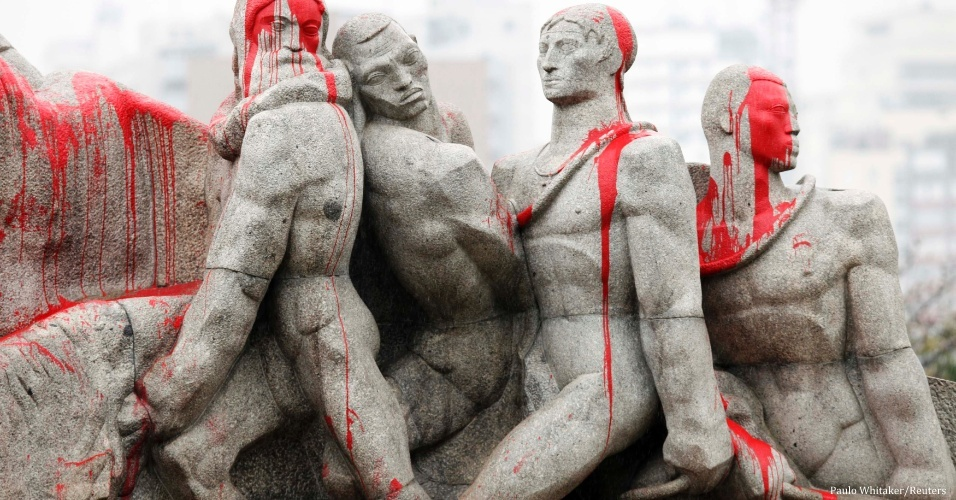
\includegraphics[width=\textwidth]{./img/GUARANIS-img2.jpg}	
  %\hfill
  %\caption{FALTANDO~LEGENDA}
\end{figure}

%\smallskip

\noindent
\emph{Para nós, povos indígenas, a pintura não é uma agressão ao corpo, mas
uma forma de transformá-lo. Nós, da Comissão Guarani Yvyrupa,
organização política autônoma que articula o povo guarani no sul
e no sudeste do país, realizamos no dia 02 de outubro
a maior manifestação indígena que já ocorreu em São Paulo
desde a Confederacão dos Tamoios. Mais de quatro mil pessoas ocuparam a
Av. Paulista, sendo cerca de quinhentas delas dos nossos parentes,
outros duzentos de comunidades quilombolas e mais de três mil
apoiadores não"-indígenas, que viram a força e a beleza do nosso
movimento. Muitos meios de comunicação, porém, preferiram noticiar
nossa manifestação como se tivesse sido uma depredação de algo que os
brancos consideram ser uma obra de arte e um patrimônio público.} 

\emph{Saindo da Av. Paulista, marchamos em direção a essa estátua de pedra,
chamada de Monumento às Bandeiras, que homenageia aqueles que nos
massacraram no passado. Lá subimos com nossas faixas, e hasteamos um
pano vermelho que representa o sangue dos nossos antepassados, que foi
derramado pelos bandeirantes, dos quais os brancos parecem ter tanto
orgulho. Alguns apoiadores não"-indígenas entenderam a força do nosso
ato simbólico, e pintaram com tinta vermelha o monumento. Apesar da
crítica de alguns, as imagens publicadas nos jornais falam por si só:
com esse gesto, eles nos ajudaram a transformar o corpo dessa obra ao
menos por um dia. Ela deixou de ser pedra e sangrou. Deixou de ser um
monumento em homenagem aos genocidas que dizimaram nosso povo e
transformou"-se em um monumento à nossa resistência. Ocupado por nossos
guerreiros \emph{xondaro}, por nossas mulheres e crianças, esse novo
monumento tornou viva a bonita e sofrida história de nosso povo, dando
um grito a todos que queiram ouvir: que cesse de uma vez por todas o
derramamento de sangue indígena no país! Foi apenas nesse momento que
esta estátua tornou"-se um verdadeiro patrimônio público, pois deixou de
servir apenas ao simbolismo colonizador das elites para dar voz a nós,
indígenas, que somos a parcela originária da sociedade brasileira. Foi
com a mesma intenção simbólica que travamos a Rodovia
dos Bandeirantes, que além de ter impactado nossa Terra Indígena no
Jaraguá, ainda leva o nome dos assassinos.}

\begin{samepage}
\emph{A~tinta vermelha que para alguns de vocês é depredação já foi limpa e o
monumento já voltou a pintar como heróis os genocidas do nosso povo.
Infelizmente, porém, sabemos que os massacres que ocorreram no passado
contra nosso povo e que continuam a ocorrer no presente não terminaram
com esse ato simbólico e não irão cessar tão logo. Nossos parentes
continuam esquecidos na beira das estradas no Rio Grande do Sul. No
Mato Grosso do Sul e no oeste do Paraná continuam sendo cotidianamente
ameaçados e assassinados a mando de políticos ruralistas que, com
a conivência silenciosa do Estado, roubam as terras e a dignidade dos
que sobreviveram aos ataques dos bandeirantes. Também em São Paulo esse
massacre continua, e perto de vocês, vivemos confinados em terras
minúsculas, sem condições mínimas de sobrevivência. Isso sim é
vandalismo.}

\emph{Esse monumento para nós representa a morte. E,
para nós, arte é outra coisa. Ela não serve para contemplar pedras,
mas para transformar corpos e espíritos. Para nós, arte é o corpo
transformado em vida e liberdade e foi isso que se realizou nessa
intervenção.}

\emph{Aguyjevete} pra todos que lutam!\footnote[*]{Carta veiculada pela Comissão Yvyrupa por ocasião da tinta
vermelha no Monumento às Bandeiras}
\end{samepage}
%\bigskip

%\begin{flushright}
%\small{Carta veiculada pela Comissão Yvyrupa\\
%por ocasião da tinta vermelha\\
%no Monumento às Bandeiras}
%\end{flushright}

\chapter*{A~caminho do Sol\\
%\bigskip
\large{\emph{Cosmografias guarani}}}

\addcontentsline{toc}{chapter}{A~caminho do Sol,
\scriptsize{\emph{por Daniel C. Pierri}}}

\begin{flushright}
\emph{Daniel Calazans Pierri\footnote{Mestre pelo \versal{PPGAS}-\versal{USP} e membro do
Centro de Trabalho Indigenista (\versal{CTI}).}}
\end{flushright}
\bigskip

\begin{quote}
\noindent
Isso que eu tenho pra contar. Então nós, Guarani, iríamos nos encontrar
frente a frente com os brancos. \emph{Nhanderu} (divindade criadora do
universo) já nos destinou para sermos \emph{tekoaxy} (seres terrestres com
corpo perecível), nos destinou para caminhar entre o lugar onde
\emph{Nhamandu} (divindade solar) se põe e o fim da terra dele
(\emph{yvyrakã}). Por isso, seguindo o caminho de \emph{Nhamandu} viemos. É~por isso
que até hoje estamos aqui. Os primeiros viveram no centro da terra (\emph{yvy
mbyte}) e vieram seguindo o caminho de \emph{Nhamandu}, porque assim é o caminho
que a alma das crianças faz, elas vêm desde onde o sol nasce, mandadas
pelos deuses para confiar e se concentrar neles. Isso tudo já acontecia
desde antes do brancos estarem aqui, já vínhamos para a beira do mar.
Então, os brancos não deveriam nem perguntar porque vivemos aqui. Nós
já sabemos disso tudo pelos \emph{nhamandu kuery} (coletividade dos \emph{Nhamandu}),
porque seguimos o caminho deles e em todo esse percurso formamos as
nossas aldeias, na direção da morada de \emph{Nhanderu}. Aqueles que vivem pra
onde o sol se põe (A~morada de Tupã), eles estão em contato com
quem está aqui, porque eles também caminham até pela beira do mar. 

\noindent
Os brancos usaram a nossa língua para dar o nome a todas as coisas que
tem nesse território: as cidades, os rios, todas as coisas estão na
nossa língua. Só isso já serviria como uma prova da nossa presença,
como dizem os brancos. Não tem como dizer que não estivemos sempre por
aqui, pois seria mentira! A~gente vai falar que é mentira, pois sabemos a
verdade. Também tem as \emph{tava} (ruínas), que eram usadas pelos Guarani.
São as ruínas, como dizem os brancos: como elas existiriam por toda
parte desse território se não fosse porque os Guarani passaram por aí? 

\noindent
Se não existisse o Guarani aqui, não existiriam essas ruínas. Tinha
aldeias grandes mesmo antigamente, bem perto de onde é o Rio de
Janeiro. Lá perto tinha 17 aldeias. Em 1500, quando os brancos
passaram, os Guarani não queriam entregar as suas aldeias e por isso os
brancos mataram muitos. São Paulo também é a mesma coisa, tinha aldeia
grande bem perto de onde é a cidade. Tudo isso aconteceu, mas como os
brancos não querem dar a terra para nós e eles são maioria, eles não
querem contar a verdade. Mesmo assim, a gente vai vencer porque a gente
tem a sabedoria dos \emph{nhanderu kuery} (coletivo genérico das divindades).
Até aqui foi a minha palavra, aqui na Aldeia Peguaoty, que vai ser uma
aldeia mesmo, bem grande.
\medskip
\begin{flushright}
\emph{Cacique Luís Eusébio}

\emph{30 de janeiro de 2011,}

\emph{Aldeia Peguaoty – Sete Barras (\versal{SP})}

\end{flushright}
\end{quote}

\bigskip
\bigskip
Essa narrativa, da qual reproduzo apenas um pequeno trecho, foi
realizada na língua guarani no contexto de um estudo para a
regularização da Terra Indígena onde se insere a aldeia na qual vive o
autor da narrativa. Trata"-se de uma aldeia do povo Mbya"-Guarani, povo
esse que ocupa uma série de fragmentos de um vasto território, que
atinge desde a região litorânea do Brasil, nos Estados de Espírito
Santo, Rio de Janeiro, São Paulo, Paraná, Santa Catarina e Rio Grande
do Sul, passando pelo interior desses quatro últimos estados e se
espalha pela região oriental do Paraguai, e pela província de
Misiones, na Argentina.

Construiu"-se em parte da literatura antropológica especializada e,
sobretudo, em parte da chamada ``opinião pública'' a ideia de que os
Guarani"-Mbya seriam um povo ``originário do Paraguai ou da Argentina''
que realizou migrações desesperadas para o litoral apenas recentemente,
inspirado por um movimento messiânico sem futuro. Todavia, existe
documentação histórica que comprove a presença dos Guarani"-Mbya no
litoral brasileiro, desde ao menos a segunda metade do século \versal{XIX}, e
nada na documentação permite afirmar com segurança que esse povo esteve
ausente do litoral em qualquer momento do período colonial.

Sem entrar nesse debate, cabe enfatizar que a narrativa acima representa
um esforço evidente de mobilizar parte do arsenal cosmológico de que
dispõe o narrador para argumentar no sentido de defender seu direito à
demarcação da terra e de se contrapor àquela visão acerca das origens
dos Guarani"-Mbya. Trata em parte, portanto, de uma mobilização política
de uma narrativa mítica. Também por isso (e nunca apesar disso) a mesma
narrativa apresenta uma série de elementos importantíssimos e complexos
para uma compreensão do que seriam as concepções cosmológicas dos
Guarani"-Mbya a respeito do espaço terrestre habitado, de sua
cosmografia e de aspectos importantes de sua cosmogênese.

Esse é o tema central deste texto, que pretende lançar luz sobre a
riqueza dessas concepções a respeito do espaço terrestre, abordando a
maneira através da qual elas são mobilizadas no discurso das lideranças
na defesa de seus direitos territoriais. Tratarei de três conceitos
nativos relacionados, todos eles mobilizados direta ou indiretamente
nessa disputa: \emph{yvyrupa} (cuja tradução literal é plataforma terrestre);
\emph{yvy mbyte} (centro do mundo) e \emph{yvy apy} ou \emph{yvy akã} (extremidade do mundo,
ou fim da terra). Os três conceitos aparecem no discurso acima, mas
pretendo principalmente contribuir para uma melhor compreensão do
conceito de \emph{yvyrupa}, porque esse foi o nome escolhido para a mais
importante organização supralocal dos Mbya: a Comissão Guarani Yvyrupa,
sobre a qual falarei brevemente ao concluir o texto.

Mas voltemos antes para o relato, para sua referência central. O~cacique
Luis Eusébio desconstrói a ideia mobilizada pelos seus adversários de
que os Guarani"-Mbya não seriam originários do litoral. Para tanto,
esclarece que os Guarani são descendentes diretos de \emph{Nhamandu}, o Sol,
que é uma das principais divindades do panteão guarani. Entretanto, para compreender o que dizia Luis Eusébio é preciso conhecer
uma outra narrativa, muito contada entre os Guarani, que é uma variante
daquela que a literatura antropológica convencionou chamar o ``mito dos
gêmeos''. Segundo ela, \emph{Nhamandu}, o Sol, nasceu na primeira terra, \emph{yvy
tenonde}, onde o seu pai, criador do universo, \emph{Nhanderu Tenonde Papa},
esteve e fecundou magicamente uma mulher que aqui vivia, \emph{Nhandexy}. Ao
se desentender com ela, \emph{Nhanderu} partiu de volta à sua morada celeste,
que ficava a Leste. Toda a história é narrada como um percurso que é
seguido por \emph{Nhamandu}, o Sol, desde que estava no ventre de sua mãe, à
procura da morada celeste de seu pai, \emph{Nhanderu}. No meio da narrativa,
sua mãe é devorada por onças, e após esse episódio Sol cria \emph{Jaxy}, o
Lua, para lhe fazer companhia como um irmãozinho. Ao fim, eles são
recebidos de volta na morada de \emph{Nhanderu Tenonde}, o pai deles, que se
situa em uma plataforma celeste localizada ao Leste.

Essa narrativa, que é uma das principais da cosmogênese desse povo, tem
para os Mbya uma territorialidade muito marcada. O~Sol ainda na barriga
da mãe, percorre a plataforma terrestre partindo do local que eles
concebem como sendo o centro do mundo (\emph{yvy mbyte}) e segue em direção ao
Leste até que atinge, já com seu irmão Lua, o fim da terra (\emph{yvy akã}).
Após o fim da terra havia nesse tempo uma outra ilha (\emph{yy paũ}), à qual
passam \emph{Kuaray} e \emph{Jaxy}, matando as onças originárias. Essa outra ilha,
que vai se separando progressivamente da terra, tornar"-se"-á uma das
moradas celestes, e esse processo de separação desemboca na criação do
mar. 

Era justamente a essa narrativa dos irmãos Sol e Lua que o cacique Luis
Eusébio se referia para dizer que os Guarani ``foram destinados a andar
do centro do mundo ao fim da terra''. Quando ele dizia que os primeiros
viviam no centro da terra e vieram ``seguindo o caminho de \emph{Nhamandu}'', há
dois sentidos a se extrair daí. Em primeiro lugar, deve"-se entender que
os primeiros são justamente Sol e Lua, \emph{Nhamandu} e \emph{Jaxy}, divindades que
os Guarani do mundo terrestre atual consideram seus antepassados e às
quais estão destinados a imitar. Em segundo lugar, esse mesmo caminho é
pensado também como qualquer trajeto percorrido na direção do sol
nascente, ao Leste, onde se situa a morada de \emph{Nhanderu Tenonde}.

O~movimento do próprio astro solar também é recorrentemente abordado
pelos meus interlocutores. Dizem os Guarani que \emph{Nhamandu}, o Sol, sai
todo dia de sua morada ao Leste iluminando a terra com um aparelho de
luz e depois o desliga e faz novamente o percurso de volta, o mesmo que
fez quando esteve na plataforma terrestre, do centro da terra ao Leste.

Mas o discurso de Luís Eusébio, ao deixar implícitas essas questões,
fala explicitamente de suas decorrências na vida concreta dos Guarani.
Ele diz que ``em todo esse percurso sempre formamos as nossas aldeias,
na direção da morada de \emph{Nhanderu}''. Ou seja, ele indica os preceitos
cosmológicos que delimitam o território de ocupação dos Guarani.
Estando os Guarani destinados a ``imitar'' os heróis da raça, como dizia
Alfred Metraux, eles devem formar suas aldeias em toda a extensão do
percurso que foi realizado no início dos tempos pelos irmãos Sol e Lua,
abrangendo desde a região central do mundo, que eles identificam ao
Paraguai e à região fronteiriça deste país com Argentina e Brasil, até
a extremidade do mundo, que é a região litorânea do Brasil. E~se foi
assim na primeira terra com os antepassados divinos dos Guarani, os
heróis Sol e Lua, sempre foi assim ao longo da história: ``mesmo antes
da chegada dos brancos'', como diz Luis Eusébio, ``já estávamos na beira
do mar''.

Entende"-se, assim, que a ideia mobilizada pelos setores contrários à
demarcação das terras guarani no litoral guarda uma consonância com a
cosmologia guarani que não passa de um mal entendido. Da mesma maneira
que seus adversários, os Guarani consideram que seus primeiros
antepassados viveram inicialmente no local que eles consideram ser o
centro do mundo, \emph{yvy mbyte}, e que coincide com alguma localidade no
Paraguai, como veremos adiante. De acordo com a sua cosmogênese, de
fato ``vieram do Paraguai''. Entretanto, os que vieram fizeram esse
percurso não nesse mundo atual, mas na primeira terra que foi destruída
pelo dilúvio, saindo do centro do mundo até a região do litoral, \emph{yvy
apy}, a extremidade do mundo. Foram os antepassados míticos Sol e Lua
que delimitaram como território de ocupação dos seus descendentes
Guarani toda a região onde hoje se estendem as centenas de aldeias
existentes.

Outra passagem da cosmogênese guarani é necessária para compreender sua
concepção de espaço. Muitos dizem que a primeira terra, quando foi
gerada por \emph{Nhanderu Tenonde}, foi gerada sobre uma grande água, na forma
de uma pequena ilha, que não tinha mais que o tamanho da planta do pé
de \emph{Nhanderu}. Posteriormente, esta ilha foi sendo ampliada e formou a
terra, ou mais precisamente o continente americano no tamanho que ele
tem hoje. Esse local onde se iniciou a terra é justamente esse centro
do mundo, \emph{yvy mbyte}, localizado provavelmente onde hoje é o Paraguai.

O~espaço terrestre é chamado \emph{yvyrupa}, termo cuja tradução literal é
suporte ou plataforma terrestre. É~dito suporte porque é concebido como
uma estrutura, dentre outras, que sustenta uma ilha concebida como um
amontoado de terra que existe em meio a um universo feito de água. A
esse respeito, transcrevo um trecho de uma outra narrativa realizada
também em guarani por um ancião de outra aldeia localizada numa ilha no
litoral de São Paulo, próxima à aldeia do autor da primeira narrativa:

\begin{quote}
\noindent
Esse mundo é grande. Em cima da terra tem um mar. E~embaixo da terra tem
um mar muito grande. Embaixo da terra é só água. É~tudo água, é mais
água que a terra. É~desse mar, que \emph{Nhanderu} pega água pra fazer chuva.
E~não é salgada. A~água que está embaixo dessa terra é maior que o mar
que a gente vê. O~mar que a gente vê é pequeno comparado com esse que
tem embaixo da terra. E~esse não é salgado.

\medskip

\noindent
(\ldots{})

\medskip

\noindent
Em cima da terra, aqui em cima, essa água é salgada, já está toda
salgada. Mas embaixo não é salgada. Então, é daí que ele pega água pra
fazer a chuva. Então, por isso que tem a nascente, essa que chega nas
cachoeiras e nos rios, ela nunca vai acabar. Elas vêm diretamente
debaixo da terra. Vêm desse mar grande, que não salgado, é de lá que
chega a nascente.

\medskip

\noindent
(\ldots{}) 

\medskip

\noindent
Já contaram pra você sobre o centro da terra? No Paraguai? \emph{Yvy mbyte}. Lá
existe a amarração da terra. É~uma corda que sai do centro da terra e
atravessa até outro mundo. De uma espécie de gancho, ele atravessa para
o outro mundo.

\noindent
Porque existem quatro mundos. No quarto mundo está \emph{Nhamandu}. É~a corda
do centro do mundo. Tem uma corda, que na verdade é um vento, é um
vento fino. E~essa corda está esticada. E~o mundo lá fica assim por
isso, lá no centro da terra é mais alto. E~pra cá ele abaixa mais, e
fica assim. E~a corda passa para o outro mundo, também pelo meio. E~lá
é o centro do mundo. É~o centro exato, lá no Paraguai. Eu não fui, mas
minha avó me contou.
\end{quote}

Essa narrativa, como a primeira, apresenta uma série de elementos
complexos a respeito de elaborações cosmológicas realizadas pelos
Guarani, que não terei espaço para abordar aqui (a esse respeito, ver
Pierri, 2013). Mas o que quero chamar atenção é que reecontramos um
tema clássico da literatura guarani, desenvolvido com detalhes não
abordados por autores como Cadogan ou Curt Nimuendaju, que lançaria
nova luz sobre as concepções guarani a respeito do espaço terrestre, de
\emph{yvyrupa}, como dizem os índios. Nimuendaju foi o primeiro autor que já
pode ser considerado um antropólogo a testemunhar os chamados
movimentos proféticos realizados por grupos guarani, saindo de regiões
interioranas para atingir à chamada Terra Sem Mal. Como é sabido, ele
dizia em suas \emph{Lendas da criação e destruição do mundo} (1987 [1914]) que
encontrou grupos guarani que saíam do sul do Mato Grosso do Sul em
direção ao litoral paulista, inspirados por líderes xamânicos para
atingir em vida a morada dos deuses. Dizia também, o que quase nunca é
notado, que embora os índios dissessem que a Terra Sem Mal se situava
além do mar, ``a maioria a leste'', alguns falavam ``de uma outra Terra
Sem Mal localizada no centro da terra''.

Ora, na narrativa que transcrevi acima, meu interlocutor nos esclarece
que existem quatro mundos, quatro plataformas, uma situada em cima da
outra, sendo a última delas a morada de \emph{Nhamandu}, o Sol. Diz também que
tanto embaixo como em cima dessa terra há uma grande água, há um mar,
que não podemos ver. Desse modo, a plataforma terrestre, \emph{yvyrupa}, é
concebida como uma estrutura que sustenta uma ilha, em volta da qual há
mar por todos os lados, por cima e por baixo. Levando isso em
consideração, a diferenciação de Nimuendaju entre uma Terra Sem Mal que
seria localizada no centro da terra e outra que estaria além do mar,
pode não fazer tanto sentido. Entre a plataforma celeste e plataforma
terrestre há água por todos os lados. Portanto, para atingir a morada
dos deuses, seja saindo do litoral, na extremidade do mundo, ou do
interior, no centro do mundo, será preciso atravessar as águas, o
grande mar que a gente não vê.

A~partir dessa concepção, esse último ancião me explicava de uma maneira
muito peculiar o que pensava sobre algo que Nimuendaju chamava de
``crença na destruição do mundo'', e que para esse autor tinha relação
direta com o profetismo. Ele me dizia que a estrutura dessa terra atual
foi reforçada depois da destruição das últimas três terras que a
precederam. Por isso, ela é segura e não vai acabar nunca. Entretanto,
\emph{Nhanderu Tenonde} está nervoso com a devastação promovida pelos brancos
e vai limpar a terra. Com isso, ele quer dizer que \emph{Nhanderu} vai varrer
toda a terra que existe em cima de \emph{yvyrupa}, da plataforma terrestre, e
renovar tudo com terra nova, destruindo a humanidade atual. O~que não
acaba, portanto, é a estrutura terrestre, o suporte da terra. 

Percebe"-se, logo, que o conceito guarani de \emph{yvyrupa} é muito mais literal
do que poderia parecer. Refere"-se de fato a uma estrutura que sustenta
a terra em que pisamos e que foi construída progressivamente a partir
do centro do mundo, onde ela está amarrada a outras estruturas que
sustentam outros mundos.

Assim como vimos que Luis Eusébio utilizava esses conceitos para rebater
argumentos de pessoas contrárias à demarcação de suas terras, \emph{yvyrupa}
tornou"-se, a partir das últimas décadas, um termo utilizado
frequentemente por grande parte das lideranças políticas guarani"-mbya
mobilizadas na luta por suas terras. Utilizam esse conceito de \emph{yvyrupa}
com o mesmo propósito que tinha Luis Eusébio no discurso transcrito no 
início, justamente para justificar seu direito à ocupação de
aldeias espalhadas pela região mais populosa do Brasil, além de
Paraguai e Argentina.

Na luta política frente ao Estado Nacional, as lideranças Guarani"-Mbya
dizem: ``os mais velhos chamam nosso território de \emph{yvyrupa}, e esse termo
quer dizer que a terra é uma só. \emph{Yvyrupa} significa mundo sem
fronteiras''.

Embora seja uma tradução que não dá conta da complexidade das concepções
de que tratamos apenas brevemente aqui, o bordão mobilizado a partir do
conceito de \emph{yvyrupa} resume boa parte das implicações que essas
concepções têm para o uso que eles fazem do espaço terrestre: grande
mobilidade territorial, ocupação de espaços fragmentados de um
território extenso, anterioridade em relação aos brancos e não
reconhecimento das fronteiras impostas pelos Estados"-nação.

Em 2006, lideranças guarani"-mbya de grande parte das aldeias situadas
nos estados de Espírito Santo, Rio de Janeiro, São Paulo, Paraná, Santa
Catarina e Rio Grande do Sul, criaram em grande assembleia, uma
organização política a qual denominaram Comissão Guarani Yvyrupa. Ela
se define pelo seu estatuto como ``uma organização indígena guarani que
foi formada para defender os direitos territoriais, garantidos pela
Constituição Federal e pelas convenções internacionais, e os interesses
coletivos do povo guarani''. O~mesmo estatuto diz ainda que ``‘Yvyrupa’ 
significa ‘leito da terra’ ou ‘a terra é uma só’''.

A~Comissão Guarani Yvyrupa formalizou um movimento que já vinha
acontecendo desde a década de 1980 em todo o litoral brasileiro,
quando as lideranças das diversas aldeias da região passaram a se
articular conjuntamente para lutar pela demarcação de suas terras, que
na maioria das vezes situam"-se em fragmentos de Mata Atlântica,
rodeados por cidades, estradas, fazendas e diversos outros
empreendimentos instalados no processo de colonização do Brasil.

A~utilização do conceito de \emph{yvyrupa} como emblema desse movimento
político é interessante porque se tratava justamente de um movimento
visando fazer com que as aldeias superassem o isolamento territorial
que foi imposto pelo Estado, reconhecendo sua luta comum enquanto um
povo único.

Para isso, optaram por utilizar esse termo que denota em sua língua todo
o espaço terrestre, onde vivem os Guarani, os brancos e uma série de
outros povos, como se significasse exclusivamente ``território guarani''.
\emph{Yvyrupa} é o território guarani, dizem. Embora seja uma aproximação,
essa tradução não deixa de denotar um aspecto central dessas concepções
que abordamos. A~devastação da Mata Atlântica e de boa parte dos
recursos naturais do planeta foi realizada pelos brancos, resultando na
expropriação do território guarani. Isso, como vimos, enervou as
divindades, antepassados dos Guarani, e elas pretendem por isso limpar
a terra, acabando com todos que estiverem aqui, índios e brancos.
Afinal, ``a terra é uma só''. Estamos todos juntos em \emph{yvyrupa}.

\section{Referências}

\begin{Parskip}
\versal{NIMUENDAJU}, Curt Unkel. \emph{As lendas da criação e destruição do mundo
como fundamentos da religião dos Apapocúva"-Guarani}. São Paulo: Hucitec/Edusp, 1987 [1914].

\versal{PIERRI}, Daniel Calazans. \emph{O~perecível e o imperecível: lógica do
sensível e corporalidade no pensamento guarani"-mbya}. Dissertação de
Mestrado. São Paulo: \versal{PPGAS}-\versal{USP}, 2013.
\end{Parskip}

\clearpage

\vspace*{\fill}

\begin{flushright}
\begin{minipage}[c]{0.85\textwidth}
\raggedleft
\footnotesize
\emph{Desde o século \versal{XVI} os Guarani tiveram uma série de tradutores, uns
melhores, outros piores, mas muita gente fazendo um esforço de
compreender esse pensamento que eles nos apresentaram. As dificuldades
começam ao tentarmos aplicar nossas categorias a esse pensamento. Uma
das questões é a ``natureza'' como separada daquilo que a gente chamaria de
``cosmologia'', ``religião'', ``metafísica'', ``cultura'', seja lá o que for. Não há
como separar. Mas por que a gente tem tanta dificuldade em afirmar
isso? Talvez porque ainda pensamos a natureza como coisa a ser
utilizada. Pierre Clastres foi um dos primeiros a apontar que um dos
problemas da expansão capitalista é não deixar o mundo à sua alegre
improdutividade, sendo preciso fazê-lo servir e render. Esse discurso
está o tempo todo rondando a briga indígena pelas terras, mas também
nossos conceitos. Felizmente algumas pesquisas atuais têm nos
proporcionado traduções melhores, falando mais nos termos guarani do
que nos nossos.}

\smallskip
\hspace*{\fill}--- Beatriz Perrone"-Moysés
\end{minipage}
\end{flushright}

\thispagestyle{empty}

\chapter*{Novas terras sem males\\
%\bigskip
\large{\emph{A luta guarani"-kaiowa pelos \emph{tekoha}}}}

\addcontentsline{toc}{chapter}{Novas terras sem males,
\scriptsize{\emph{por Spensy K. Pimentel}}}

\begin{flushright}
\emph{Spensy K. Pimentel}\footnote{Docente na Universidade Federal do Sul da
Bahia. Este artigo amadureceu a partir de diálogos com o historiador
kaiowa Izaque João e o \emph{nhanderu} Atanásio Teixeira, a quem agradeço
imensamente pela oportunidade de diálogo. O~presente texto constitui um
desdobramento de reflexões iniciadas em Pimentel (2012a), sobretudo a
partir de uma entrevista, citada em ambos os textos, que foi gravada
com o sr. Atanásio para o vídeo ``Mbaraka --- A~Palavra que Age'',
realizado em parceria com Edgar Teodoro da Cunha e Gianni Puzzo a
partir do prêmio Etnodoc 2009. Na tradução das entrevistas para o
vídeo, agradeço especialmente pelo apoio de Eliel Benites e Graciela
Chamorro.} 
\end{flushright}

\noindent
Os Guarani"-Kaiowa\footnote{No contexto sul"-matogrossense, os
Guarani"-Kaiowa costumam usar a designação ``Kaiowa e Guarani'',
diferenciando os falantes do dialeto kaiowa e os do dialeto nhandeva ---
localmente, estes são denominados Guarani. Em outras regiões, vale
notar, o jogo de etnônimos é distinto.} angariaram solidariedade
nacional e internacional nos últimos anos em função da repercussão na
internet e meios de comunicação tradicionais das notícias sobre a luta
ferrenha e desigual que esse grupo indígena trava pela demarcação de
suas terras na região sul de Mato Grosso do Sul.

Desde os anos 1980, têm sido frequentes as denúncias envolvendo, por um
lado, mortes de lideranças e despejos violentos em retomadas de terra
e, por outro, um cotidiano de fome, violência e suicídios nas antigas
reservas demarcadas pelo Serviço de Proteção ao Índio, as quais se
encontram superlotadas e em péssimas condições políticas, econômicas e
sociais (Pimentel, 2010; Pimentel \& Moncau, 2011).

Conhecido como \emph{Aty Guasu} --- Grande Assembleia Kaiowa e Guarani, esse
movimento de luta pela terra envolve reuniões periódicas com centenas
de lideranças, que costumeiramente divulgam uma declaração final em
português. Antigamente entregues às autoridades de órgãos como
Ministério Público Federal e Fundação Nacional do Índio (\versal{FUNAI}), hoje,
esses textos ganham grande divulgação via internet.

E, pois, lê-se no documento final de uma recente \emph{Aty Guasu}:

\begin{quote}
\noindent
Não vamos tolerar mais essa demora (nas demarcações de terra) e vamos
nos organizar cada vez mais para retomarmos nossas terras, custe o que
custar. E~que o sangue de nosso povo semeie as nossas terras sagradas
para renascer a esperança de alcançarmos a terra sem males
(\ldots{})\footnote{Documento final da \emph{Aty Guasu} realizada na aldeia Paso
Piraju (Dourados"-\versal{MS} --- Terra Indígena em processo de identificação),
datado de 21/8/2011.}
\end{quote}

Não se trata de um exemplo único. O~uso do termo ``terra sem males'' é
corriqueiro nos documentos ligados às \emph{Aty Guasu}. No discurso político
do movimento, a associação entre as áreas a serem demarcadas e a Terra
sem Males é uma constante. O~termo correspondente, em guarani, é mesmo
\emph{Yvy Marane’y}, algo simples de verificar no diálogo com as lideranças.

Como pensar, então, essa \emph{Yvy Marane’y} à qual não se chega a partir de
uma longa caminhada até a beira da plataforma celeste, tal como boa
parte da literatura etnológica em torno dos Guarani desenvolveu ao
longo do século \versal{XX}? Que terra sem males é essa que se pode acessar
rompendo a cerca dos latifúndios sul"-matogrossenses?

Formam um denso emaranhado as associações que os textos etnológicos
fizeram, ao longo do século \versal{XX}, em torno desse que se tornou um dos
grandes temas guarani, a Terra sem Males, \emph{Yvy Marane’y}.

Noelli (1999) rememorava"-nos o longo processo, por meio do qual se
teceram hipóteses cada vez mais abrangentes --- e arriscadas --- sobre a
Terra sem Males e, particularmente, sua associação com a mobilidade
guarani. O~autor destaca, na criação do que chama de ``mito acadêmico''
(1999: 123), as obras de Nimuendaju (1987 [1914]) e Métraux (1927).

Em resumo: o pioneiro Nimuendaju encontra, em 1912, uma família guarani
dirigindo"-se a pé para a Serra do Mar, no litoral atlântico brasileiro.
Eles --- que, ao que tudo indica, já haviam viajado por centenas de
quilômetros rumo ao Leste --- lhe dizem que fazem esse caminho para
tentar chegar, em vida, à Terra sem Males, \emph{yvy marane’y}, um lugar ``onde
não mais se morre''. O~autor elucubra: e se, de modo geral, as migrações
tupi"-guarani anteriores à conquista fossem também uma busca por esse
paraíso terreal? (1987: 107).

A~hipótese de Nimuendaju começa a ser dada como favas contadas, cresce
mais e mais, sobretudo a partir de Métraux, que a ``reforça e
amplifica'', na avaliação de Noelli (1999: 136). Talvez, o exemplo mais
significativo sobre a dimensão que tomaram os imaginados ``motivos
religiosos'' para os movimentos coletivos guarani esteja na análise que
se construiu a respeito do termo \emph{kandire}.

Autores como Viveiros de Castro (1995: 247, 371) ou Pissolato (2007:
410-11) --- entre muitos outros, diga"-se de passagem --- tomam, a partir de
Hélène Clastres (1978), certa glosa de Cadogan a respeito da expressão
\emph{oñemokandire}, constante de um dos cantos mbya compilados pelo autor no
\emph{Ayvu Rapyta}: descrever"-se"-ia, aí, ``el tránsito de la inmortalidad sin
sufrir la prueba de la muerte, es decir, la ascensión al cielo después
de purificar el cuerpo mediante los ejercicios espirituales'' (Cadogan,
1997: 101). 

Tratar"-se"-ia, pois, de um elemento central no conjunto de ideias que
resultaria na proposta de Viveiros de Castro, com a noção de uma
``ambivalência do humano'' (Pissolato, 2007: 410) posta em destaque nas
cosmologias tupi"-guarani. Esse autor, como se sabe, considerava a ideia
de um ``modelo tupi"-guarani'' (1986: 623-700), elaborado a partir de uma
comparação entre os Tupi seiscentistas, os Guarani e os Araweté --- bem
como de alguns paralelos com outros grupos tupi amazônicos
contemporâneos.

Em tal constructo, a ``metafísica tupi"-guarani'' envolvia uma concepção de
pessoa constituída pelo ``devir'' (1986: 623). Entre os Guarani,
especificamente, a concepção da pessoa como devir se expressaria no
\emph{aguyje}, que consiste no ideal xamânico de, por meio do aperfeiçoamento
corporal/espiritual, alcançar a imortalidade/ ``amadurecimento''.
Viveiros de Castro recupera aí Hélène Clastres (1978), autora que
associava uma suposta passagem das migrações guarani documentadas no
século \versal{XVI} --- já entendidas como uma procura da Terra sem Males --- à
ascese xamânica da busca pela perfeição individual, o \emph{aguyje}, capaz de
levar a esse paraíso em vida, como se tivesse ocorrido um processo de
``interiorização'' da busca pela \emph{Yvy Marane’y}\footnote{Essa configuração
de uma teoria guarani da pessoa, de fato, remonta ainda à obra de
Nimuendaju, que, em seu relato sobre a crença na duplicidade da alma
entre os Apapokuva (1987: 29-47), já apontava para essa ``visão dual da
pessoa'' (Viveiros de Castro, 1987: xxvii).}.

Cadogan, nessa mesma passagem citada, indica, porém, um fato"-chave. ``Es
sugestivo que a una nación no guarani se haya designado en la época de
la conquista con este nombre Kandire. Se los habrá considerado como
inmortales por poseer una cultura superior?'' (Cadogan, 1997: 101). E,
se, para além de um conceito relativo à cosmologia, tratava"-se de um
termo aplicado a um ou mais grupos com o qual ou os quais os Guarani
mantinham contato e que, por sua cultura característica, inspirava(m)
essa associação, de quem se estaria falando?

Recentemente, Combès e Julien são duas autoras que retornaram a esse
enigma dos \emph{Kandire}, referidos nos documentos coloniais. Elas recuperam
uma série de documentos quinhentistas a respeito do deslocamento de
grupos de língua guarani ao longo da bacia do Prata, rumo à região do
piemonte andino, nas proximidades do que hoje é Santa Cruz de La
Sierra, na Bolívia, demonstrando evidências de que, longe de
representar, simplesmente, uma ``reação à conquista'', essas
movimentações --- há muito conhecidas, mas ainda pouco estudadas ---
indicam a existência de uma grande rede de trocas, alianças e
hostilidades, implicando um fluxo intenso de pessoas e bens,
particularmente a presença de objetos de metal andino circulando por
toda a área. Ou seja, um panorama bem menos compatível com a hipótese
de ``motivos religiosos'', ou ``levantes político"-místicos'', como
sintetiza Julien (2007: 265).

As explicações para essa movimentação guarani, segundo tal autora,
apontam muito mais para a busca por metais e a ânsia por resgatar
parentes presos em expedições anteriores --- o que, para Julien,
demonstra que, em vez de falar em migrações guarani rumo aos Andes,
seria mais produtivo perceber que se tratava de enormes redes de
alianças e hostilidades, que inclusive ultrapassavam em muito as
barreiras linguísticas (idem: 251, 254).

Nesse contexto, como aparece o termo \emph{kandire}? As autoras demonstram que,
em vários documentos, trata"-se mesmo de um grupo, não um lugar --- os
Kandire\footnote{Nos documentos e, por conseguinte, nos textos de
Combès e Julien, é frequente que se grafe o termo como Candire --- aqui,
usarei genericamente kandire, adequando"-se à grafia utilizada no
guarani contemporâneo.}, portanto, como já percebia Cadogan ---, e que o
termo se referiria aos Inca. Seriam os ``señores verdaderos del metal
amarillo'', ou seja, o ouro (Combès, 2011: 102). Mais precisamente,
Combès argumenta que as menções aos Kandire se refeririam aos Inca da
região de Samaipata --- fortaleza construída para defender minas de prata
exploradas pelos andinos na região próxima a Santa Cruz. Os Carcaraes,
outro grupo também citado nos documentos, seriam \emph{mitimaes}
(funcionários) empregados pelo inca Condori nessas minas conhecidas
como Saypuru --- a própria designação Kandire poderia ser derivada de
Condori, supõe (2011: 102-3).

A~autora busca refinar as hipóteses de Julien --- não é que se deva opor
os ``motivos religiosos'' de Nimuendaju a um cálculo e uma razão ``à
ocidental'', que justifica a movimentação registrada na bacia do Prata a
partir de motivações materiais. ``Una ‘tierra
rica’ de metal bien puede a la vez ser tierra de
‘cosas buenas’'', conjectura ela
(2011: 103-4).

Combès lembra que Métraux já apontava para uma convergência entre as
buscas pela mítica Terra sem Males e os Inca --- da mesma forma que
Saignes percebia que esses movimentos tinham algo a ver com a busca por
metais. Mais recentemente, isso não passou despercebido a autores como
Monteiro (1992) e Carvalho (1992), mas o fato é que não se tiraram
consequências práticas da existência desses dados para a caracterização
dos coletivos indígenas que atuam na história da região, bem como de
seus movimentos e redes de circulação.

O~que está em jogo aqui é a oposição cartesiana entre sagrado e profano,
ou entre razão prática e razão simbólica. Tudo era concomitante, e não
havia contradição nisso. ``En cuanto a la búsqueda del metal andino, se
trata al parecer de un afán demasiado
`materialista' para caber en la
imagen idealizada de un paraíso terrenal'', ironiza Combès, em outro
texto (2011b: 27).

As viagens guarani rumo ao Oeste (sejam migrações ou expedições) são um
tema pouco explorado na bibliografia etnológica sobre os Guarani.
Menções a elas são feitas, mas sem maiores detalhes sobre suas
motivações\footnote{Veja"-se, por exemplo, Meliá, Grünberg e Grünberg,
(2008: 16-7), ou Meliá (1993). Mesmo quando se menciona essa questão,
como em Monteiro (1992: 484), pode parecer que os grupos guarani
simplesmente seguiam os europeus que buscavam o metal. }. A~discussão
clássica, em geral projetada ao passado, oscilou entre considerar as
antigas migrações tupi"-guarani como ``crises messiânicas'' (Métraux,
1979: 175), oriundas da ``aculturação'', com a chegada dos europeus, ou,
nas obras de Pierre e Hélène Clastres, como um ``processo autóctone'',
relacionado ao crescimento demográfico\footnote{Gloso aqui a leitura
que Pissolato (2007: 99-105) faz desse debate. Sztutman, por sua vez,
rejeita o termo ``messianismo'', mas continua centrando a discussão no
``profetismo'' como ``xamanismo feito história'' (2005: 410) ou ``leitura da
história'' (op.cit.: 430) feita pelos povos indígenas. No caso
chiriguano, ele foca sua análise na obra de Saignes a respeito da
história do grupo desde o período colonial e a emergência dos profetas
\emph{tumpa}, que se contrapunham aos \emph{mburuvicha}.} e consequente expansão
geográfica, que acirraria uma ``contradição entre o político e o
religioso'' (H. Clastres, 1978: 45): grandes chefes com prestígio em
escala cada vez maior, espécie de ``força centrípeta'', enquanto os
profetas agiriam de forma ``centrífuga'', numa ação ``contra o Estado'',
utilizando a expressão de Pierre Clastres\footnote{E~por essa passagem
se percebe que H. Clastres também percebia essa ambiguidade citada por
Combès, entre ``razões ecológicas e econômicas'' e ``razões de ordem
mítica'' (H. Clastres, 1978: 59).}.

O~problema que está posto aqui é o seguinte: será mesmo que, quando
estamos falando de Terra sem Males, nos referimos a algo que está no
polo do divino, do religioso, de um ``não ser social'', de ``forças
negadoras do social'' (H. Clastres, 1978: 45), ou, como afirmou, mais
recentemente, Sztutman, de uma ``tradução guarani do devir não humano''
(Sztutman, 2005: 41)?

No Brasil, os Kaiowa e Guarani de Mato Grosso do Sul representam a
maioria absoluta dos atuais grupos de língua guarani. Eram, em 2013,
46,3 mil pessoas, habitando 30 Terras Indígenas e cerca de outros 35
acampamentos --- muitos em beira de estrada, alguns dentro de fazendas
ocupadas para pressionar contra a morosidade na demarcação de
terras\footnote{Os dados de população são da Secretaria Especial de
Saúde Indígena (Sesai). Afora os Guarani Kaiowa de Mato Grosso do Sul,
há, no Brasil, outros 12,5 mil Guarani, de acordo com a mesma fonte. A
informação sobre os acampamentos foi recolhida pelo Conselho
Indigenista Missionário, em 2011. As Terras Indígenas, note"-se, não
estão todas completamente ocupadas --- há casos em que os indígenas
esperam pela resolução de conflitos judiciais em apenas uma pequena
porção da terra já demarcada, ou mesmo homologada (vide os casos
Nhanderu Marangatu e Arroio Korá, que aguardam, há anos, por decisões
do Supremo Tribunal Federal).} ---, além da periferia de cidades da
região.

Essa população conforma, hoje, o segundo maior grupo indígena do
Brasil\footnote{Se considerados em conjunto com os grupos guarani de
outros estados, estamos falando do maior povo indígena do país, com
aproximadamente 58.800 pessoas (Sesai 2012a).} --- e o maior povo
indígena fora da Amazônia ---, mas tem à sua disposição pouco menos de 50
mil hectares de terra, efetivamente. Há algo em torno de 40 mil
hectares, aproximadamente, já reconhecidos como terras de ocupação
tradicional, mas ainda em poder de fazendeiros, em função de arrastadas
disputas judiciais. 

Desde 2008, após anos de pressão do Ministério Público Federal, a
Fundação Nacional do Índio iniciou um processo, ainda inconcluso, para
identificar e delimitar como terras guarani"-kaiowa outras 39 áreas,
pelo menos, as quais, numa estimativa inicial, somariam algo em torno
de 600 mil hectares\footnote{Atualmente, trava"-se uma pesada discussão
sobre como se poderá efetivar a posse dessas terras para os indígenas,
pois grande parte das áreas está ocupada por fazendeiros que detêm
títulos de terra concedidos, décadas atrás, pelos governos federal ou
estadual. Cf. Pimentel, 2010 e 2012; Pimentel \& Moncau, 2011.}. 

Cada uma dessas áreas pleiteadas pelos Kaiowa e Guarani é conhecida como
\emph{tekoha} --- significando algo como ``o lugar onde se pode viver do nosso
próprio jeito''. Da forma como é usado hoje, o termo é uma objetivação
que surgiu no âmbito das discussões sobre a demarcação de terras, desde
os anos 80. 

Do lado paraguaio, Melià, Grünberg e Grünberg (2008) tinham registrado o
uso do termo no âmbito do debate sobre a regularização de terras
paĩ{}-tavyterã\footnote{Autodenominação mais comum dos indígenas
falantes de kaiowa que vivem do lado paraguaio.}, ocorrido por lá
sobretudo nos anos 1970. A~despeito disso, como se sabe, palavras
correlatas são muito comuns, não só na história guarani (vide a obra de
Montoya), como em outros povos de línguas tupi"-guarani. Por exemplo,
Gallois (2004) registra, entre os Zo’e, coletivo tupi amazônico do
noroeste do Pará, contatado nos anos 1980, a emergência do termo \emph{zo’e
rekoha}, aplicado à Terra Indígena Zo’e, durante o processo de
reconhecimento territorial pelo qual o grupo passou. 

No contexto atual, em Mato Grosso do Sul, o termo \emph{tekoha} indica uma
porção de território com o qual um determinado coletivo kaiowa ou
guarani consegue identificar uma relação que pode ser interpretada
pelos não indígenas como de ``ocupação tradicional'', ao mesmo tempo em
que percebe, ali, os elementos necessários para restabelecer o chamado
\emph{teko porã}, o bom modo de ser, o modo de ser dos antigos, fugindo às más
condições que imperam nas antigas reservas demarcadas pelo \versal{SPI}, onde ---
sobretudo em função de se viver ``misturado'' (\emph{jopara}) com os \emph{karai} (na
proximidade das cidades) e da falta de alegria (\emph{vy’a}) resultante da
miséria (por sua vez relacionada, sobretudo, à superlotação e aos
problemas ambientais) --- impera um \emph{teko vai} (modo de ser ruim, ou
imperfeito).

Essa forma de orientar a luta contra a colonização guarda forte
continuidade com outros momentos históricos entre grupos guarani. O
esforço dos xamãs kaiowa e guarani, hoje, como há vários séculos, é o
de pregar a volta ao \emph{nhande reko}, seu modo próprio de ser, de agir.
``Pegar o jeito do branco'', uma expressão comum de se ouvir, é o perigo.
O~\emph{nhande reko}, o jeito kaiowa/guarani de ser, de fazer as coisas, está
intimamente ligado às práticas xamânicas. Retomar as áreas de \emph{tekoha} é
recuperar hábitos e práticas dos antigos, hoje impossibilitadas pelo
ambiente (cada vez mais) urbano das grandes reservas.

Essas práticas dos antigos, justamente, dependem de elementos que nós
designamos por ``natureza''. Nesse sentido, mais uma vez, há uma relação
direta entre a luta pela terra, o xamanismo e a política. Terra, aqui,
é muito mais do que o mero suporte para a ``produção'' que nela veem os
brancos. De todo modo, o fato é que o projeto, teoria ou filosofia
kaiowa da política passa, de forma decisiva, por aquilo que chamamos de
natureza. E~isso não apenas no sentido ``romântico'' identificado pelos
fazendeiros, de uma ``volta à natureza''\footnote{Esse termo é
constantemente evocado pelo \emph{establishment} ruralista em \versal{MS} para
questionar o sentido do movimento indígena de luta pela terra (cf.
Pimentel, 2012a e 2012b).}. Mais que um objetivo, a natureza é aliada
no processo de luta pela terra (cf. Pimentel, 2013).

Animais, plantas, elementos do clima (como ventos e raios) e da paisagem
(morros, rios, lagos), que servem como morada para certos seres, são
considerados manifestações deles ou são elas mesmas entidades
participantes da luta pela terra. A~forma mais genérica de denominar
essas ``entidades sensíveis'' (De La Cadena, 2008), que são aliados,
parentes, ou mesmo ancestrais dos Kaiowa e Guarani é, como se viu,
\emph{Tekojára}, os ``donos do nosso modo de ser'', numa das possíveis
traduções. Nesse sentido, o que está em jogo, na luta pela terra, é a
expectativa de voltar a ocupar um espaço onde possam relacionar"-se, da
forma apropriada, com todos esses seres"-elementos citados (cf. Pereira,
2004).

A~ideia de abandonar a ordem imposta pelos brancos e retomar os ``antigos
costumes'', ou os costumes próprios, como fundamento das rebeliões tupi
e guarani, é reiteradamente citada em documentos coloniais e,
evidentemente, transformada ao longo da história, persiste até os dias
atuais. Significativamente, porém, dançar e cantar continuam sendo atos
fundamentais na retomada dos ``bons costumes'' (\emph{teko porã}), e subversivos
aos olhos de boa parte dos brancos da região onde habitam, tal como nos
tempos do profeta Oberá, que liderou uma rebelião guarani em 1579 (cf.
Meliá, 1993).

O~pensamento de um dos expoentes do movimento \emph{Aty Guasu}, o
\emph{nhanderu}\footnote{Um dos termos mais comuns que os Kaiowa costumam usar
para designar os xamãs --- ``nosso pai''. No litoral, entre os
Mbya/Nhandeva, designa o Criador do Mundo. Para diferenciar os xamãs
deste personagem, os Kaiowa chamam"-no \emph{Nhanderuvusu} --- ``nosso pai
maior''.} Atanasio Teixeira, é exemplar no sentido de aclarar de que
forma os \emph{tekoha} são pensados como \emph{yvy marane’y}. Além de gozar de grande
credibilidade como curador e de ser considerado hoje um dos poucos
conhecedores de diversos rituais que já não são mais realizados na
maior parte do território kaiowa/guarani do lado brasileiro, em função
da degradação ambiental, Atanásio é um \emph{nhanderu} de extrema importância
na construção do movimento de luta pela terra. 

Nos anos 1980, ele e outro xamã, o guarani Delosanto Centurión, morto em
2009, foram as principais figuras em um momento histórico decisivo:
diante de uma série de impasses no processo de regularização das terras
então reivindicadas, entre 1985 e 1986, eles passaram a criticar a
forma como agiam as lideranças que então estavam à proa das ações de
luta.

Para eles, era preciso retomar o modo antigo de encaminhar a resolução
dos problemas, cantando e dançando para pedir a benção e o apoio dos
deuses, orientando o movimento de luta pela terra de acordo com as
instruções recebidas no processo de diálogo xamânico com essas
entidades\footnote{Para um debate sobre o princípio cosmopolítico que
embasa essas formulações, a ideia de que o xamã ideal é aquele que vê o
futuro, recebendo a denominação de \emph{johexakáry}, ver Pimentel (2012: cap.
3).}. Nesse período, os dois, junto com outros xamãs, conseguiram apoio
do movimento indígena para promover, a partir de 1987, as chamadas
\emph{Jeroky Guasu} (grandes danças/rezas). Foi a partir dessa fase que
surgiu, pouco depois, o formato que é verificado até hoje para as
assembleias \emph{Aty Guasu} (cf. Pimentel, prelo).

Até hoje, Atanásio participa ativamente do movimento \emph{Aty Guasu}, e sua
voz é ouvida com extrema deferência nas assembleias. Em uma entrevista
com ele realizada em 2010\footnote{Para o vídeo ``Mbaraka: a palavra que
age'' --- \emph{https://vimeo.com/34768557}. O~texto
final da tradução deve"-se especialmente a Eliel Benites e Graciela
Chamorro.}, assim se referia ao que irá acontecer quando os Kaiowa e
Guarani conseguirem ocupar efetivamente as terras que hoje reivindicam:

\begin{quote}
\noindent
Então, haverá dança e caminhada até o lugar onde vai renascer a nossa
terra, e é ali que nós vamos. Ali haverá novamente os que vão dançar,
vão ser arrumadas as casas. Então, nesse lugar eles vão abençoar,
trazer coisas boas. Depois de abençoar o lugar, eles (os \emph{Nhanderu}) vão
poder trazer de volta as nossas caças, o dono da caça vai chamar os
animais, eles vão baixar de novo.
\end{quote}

As festas kaiowa e guarani, segundo a memória dos mais velhos, estavam
relacionadas a um tempo de fartura, antes do desmatamento massivo na
região e do confinamento, quando as colheitas eram abundantes, e as
famílias podiam convidar periodicamente os vizinhos para cantar, dançar
e pedir aos deuses por sua saúde e a alegria. Esses rituais, como a
nominação das crianças (\emph{nimongarai}) ou a passagem dos meninos à idade
adulta (\emph{mitã pepy}), sinalizada antigamente por um furo na parte
inferior da boca, o \emph{tembekua}, onde se instalava um fio de resina de
certa árvore, o \emph{tembeta} --- estão entre as mais fortes lembranças de
Atanásio, e compõem o cenário da terra almejada, onde os parentes um
dia poderão voltar a viver do seu próprio jeito, o \emph{nhande reko}:

\begin{quote}
\noindent
Então haverá novamente o convite à cerimônia das crianças (\emph{mitã pepy}),
haverá novamente a celebração do \emph{tembekua}, haverá novamente a dança
(\emph{jerosy}), o canto longo (\emph{mborahei puku}), pra trazer de volta a festa do
milho verde (\emph{avati kyry}). Vão ser abençoados (\emph{hovasa}) os canaviais, os
mandiocais, as crianças. Vamos ter novamente ali todas as coisas, o
novo lugar vai ser fortalecido com as rezas, ali não será mais preciso
ter outro modo de viver. Ali haverá uma nova vida com danças, vida
sadia, e vida em abundância.
\end{quote}

Como se pode ver, a descrição feita por Atanásio desse cenário de
abundância que se aguarda para o momento de recuperação das terras se
aproxima muito da que se costuma fazer no contexto do movimento
indígena. Os \emph{tekoha}, portanto, são cenário de uma promessa de fartura,
alegria e festa. O~discurso político, aqui, como já destacamos alhures
(Pimentel, 2012b), se torna uma espécie de profecia, uma vez que, no
pensamento político kaiowa e guarani, a presença dos xamãs nas ações
coletivas é um dos fatores determinantes para o sucesso de qualquer
empreitada. É~o xamã quem deve dar o aval definitivo para qualquer
movimentação expressiva de um coletivo, ou, caso contrário, haverá
sérios riscos de fracasso. 

É~nesse sentido que parece ser cada vez mais adequado deslocar a
discussão sobre o xamanismo guarani, que, não poucas vezes, foi
encaminhada para o campo da religião\footnote{Deve"-se fazer a seguinte
ressalva: no contexto local, para os próprios indígenas, ainda costuma
ser bastante relevante discutir a questão do xamanismo como opção
religiosa, em função da perseguição ferrenha que sofrem os \emph{nhanderu} e
\emph{nhandesy} e seus familiares, por parte, sobretudo, das igrejas
evangélicas pentecostais --- as quais se contam às dezenas, em áreas como
a de Dourados.}. É~oportuno pensar aí no que vem sendo escrito sobre
a ideia de cosmopolítica\footnote{Cosmopolítica seria a ``nova
política'', no dizer de Latour (2001: 347) --- a política livre do acordo
moderno que isolava a natureza, como se a ela não dissessem respeito as
decisões políticas. Por si só, esse acordo já definia um ``cosmos'' para
uma certa política. Novos cosmos, novas políticas.}, ou ``política
ontológica'', como aponta Mol: 

\begin{quote}
\noindent
A~combinação dos termos ``ontologia'' e ``política'' sugere"-nos que as
condições de possibilidade não são dadas à partida. Que a realidade não
precede as práticas banais nas quais interagimos com ela, antes sendo
modelada por essas práticas (Mol, 2008: 63).
\end{quote}

O~deslocamento que propomos nos parece útil no sentido de desfazer um
equívoco recorrente: enquanto tantos estiveram endossando os ``motivos
religiosos'' das migrações guarani históricas\footnote{Somente Meliá
(1989) ousou levar às últimas consequências essa discussão, sugerindo o
que, aqui, estamos constatando operar plenamente na atualidade: a
associação entre a ``terra ideal'' e a terra almejada, disputada e
conquistada aqui mesmo, neste mundo.}, Atanásio e a Aty Guasu nos
lembram que essas dimensões estão, como parecem sempre ter estado,
completamente mescladas, que não é possível separá-las. Diferente do
que percebe H. Clastres para os Tupinambá seiscentistas, não se trata
de um choque entre ``razões econômicas'' e ``razões míticas'': os vetores
se reforçam, não se opõem.

Igualmente, na bibliografia a respeito dos Guarani do litoral, diversos
autores enfatizaram, nas últimas décadas, a motivação originalmente
``religiosa'' das migrações guarani. Diante da persistência, em certos
segmentos sociais, da ideia de que os indígenas eram ``invasores
paraguaios'', ameaçando as áreas de conservação na Serra do Mar,
antropólogos que identificavam uma ``resistência'' em reconhecer a
relação dessas migrações guarani com o tema da Terra sem Males e a
reprodução dos caminhos trilhados pelos ``grandes heróis ‘divinizados’''
(Ladeira, 2007: 66), lograram demonstrar que essa dimensão profética
das migrações permanecia viva na memória de muitos idosos. 

Em \versal{MS}, como no litoral, trata"-se, portanto, de reconhecer que as
dimensões político"- territoriais e cosmológicas estão imbricadas. Em
ambos os casos, pois, emerge uma discussão que poderíamos caracterizar
como cosmopolítica.

Há uma tendência, contudo, que se deveria evitar, para que o
deslocamento cosmopolítico se efetive. Diante de apontamentos como os
de Noelli, supracitados, Chamorro também reconhece a necessidade de que
se sublinhem as dimensões sócio"-históricas ligadas ao tema da Terra sem
Males. ``Tanto as causas do medo da destruição do mundo são eventos
sócio"-históricos como a busca de uma ‘terra sem males’ não é
necessariamente uma fuga da realidade terrena para as esferas celestes,
pois é também a busca de uma terra tão real quanto necessária'', diz ela
(Chamorro, 2010: 102). 

A~questão é que ela remete a relação aqui apontada a um campo político
muito específico, o das utopias: ``As utopias e os mitos não dizem
respeito só ao mundo espiritual e os acontecimentos histórico"-sociais,
são a base da dimensão transcendente da religião'' (idem). Chamorro não
foi a única a utilizar o termo ``utopia'' associado à Terra sem Males.
Carneiro da Cunha e Viveiros de Castro (2009[1985]: 95) igualmente o
fizeram. 

Por que, afinal, é que, mesmo quando reconhecemos a dimensão política da
Terra sem Males, vamos considerá-la uma ``utopia''? Utopia, afinal ---
assim como mito ---, é um termo associado ao improvável, ao sonho, à
fantasia. No Mato Grosso do Sul de hoje, é frequente que os fazendeiros
e seus apoiadores (na política, na imprensa) se refiram desse modo às
pretensões dos indígenas de recuperarem suas terras de ocupação
tradicional. Imaginar que poderão transformar aquelas áreas hoje
completamente desmatadas e estéreis em plantações e florestas onde se
recuperará a biodiversidade e o modo de vida dos antigos é impossível,
dizem os que se opõem aos Kaiowa e Guarani.

Pode ser que o complexo de ideias em torno da \emph{Yvy Marane’y} tenha
apresentado tal sentido em alguma de suas transformações registradas ao
longo destes cinco séculos, mas o fato é que, hoje, em Mato Grosso do
Sul, são as terras a serem demarcadas, os \emph{tekoha}, que se tornaram a
autêntica Terra sem Males a que almejam os Kaiowa e Guarani,
literalmente alcançável pela ação política planejada e consciente, e o
único horizonte que muitos desses indígenas vislumbram para que se
possa recuperar uma sociabilidade minimamente aceitável, que
proporcione uma vida plenamente humana.

Diante dessas constatações, resta"-nos, penso, refletir sobre o sentido
dessa nossa recusa a reconhecer como devir humano essa espécie de
movimento político --- pois, afinal, é em condições absolutamente
subumanas que os Kaiowa e Guarani têm sido obrigados a sobreviver nas
últimas décadas\footnote{E~isso, em suas próprias palavras: é comum, no
âmbito do movimento Aty Guasu, que as lideranças comparem a situação
dos Kaiowa e Guarani nas reservas com a de porcos presos num
chiqueiro.}. Por que é que esse tipo de movimento fica confinado, na
bibliografia, ao campo do religioso, da utopia?

Um recente debate, justamente, nos ajuda a pensar a respeito disso. Em
2008, o então ministro da Secretaria de Assuntos Estratégicos,
Mangabeira Unger, foi questionado, em entrevista\footnote{Publicada em
\emph{O~Globo}, 27/5/2008.}, se achava que os índios já não teriam terra
demais no Brasil. Ele respondeu dizendo que o destino do homem não
podia ser o de permanecer como uma ``criança aprisionada em um paraíso
verde'' e que, apesar de disporem de uma porção ``generosa'' de terra, os
indígenas no país não têm acesso a ``oportunidades econômicas''. Isso
deveria ser ``consertado'', em função do compromisso do país com os
índios, que, como todas as pessoas, ``são espíritos que desejam
transcender''.

Viveiros de Castro publicou na internet uma resposta a Mangabeira, a
partir da qual, posteriormente, compôs um texto juntando"-a a outros
escritos (2011). Para o autor, a Amazônia não poderia ser considerada
um ``paraíso'' --- ou seja, algo concedido por um poder superior, sendo,
isto sim, uma ``laboriosa construção co"-adaptativa'', resultado da
interação entre a ``engenhosidade técnica'' dos indígenas e as
``engenhosidades naturais'' das espécies da região. 

``Deixemos o paraíso para quem precisa de paraíso'', diz ainda, defendendo
a tese de que as culturas e sociedades indígenas escolheram um ``caminho
civilizacional radicalmente distinto do nosso'', uma ``via da imanência''
--- em lugar de uma ``via da transcendência''. ``Os índios são os senhores
da imanência: o que nós não podemos, se não pensar, eles vivem. E~o que
eles pensam, nós não somos mais capazes sequer de imaginar'', lança,
ainda, o autor.

Mas, afinal, tantos na academia não estiveram, justamente, enxergando a
\emph{Yvy marane’y} como um lugar da transcendência ao longo do século \versal{XX}? Não
foi esta nossa tradição de saber que aplicou, aí, algo parecido a essa
ideia de Mangabeira de que ``todas as pessoas são espíritos que desejam
transcender''?

Na prática, houve outra instituição que não a universidade ou o
indigenismo estatal (\versal{SPI}, \versal{FUNAI}), que se encarregou de, diretamente,
repassar aos indígenas uma mensagem a respeito de nosso ``caminho
civilizacional'' e das opções que ele permitira aos Kaiowa e Guarani. 

Igrejas cristãs, justamente, estiveram, ao longo do século \versal{XX}, entre as
pioneiras no processo de confinamento desses indígenas. Segundo
relatos, em diversos lugares do sul de \versal{MS}, as missões evangélicas
desempenhavam o papel de promotoras dos benefícios do ``aldeamento''. Os
agentes religiosos convenciam os indígenas de que, junto às missões,
dentro das reservas criadas pelo \versal{SPI}, eles contariam com benefícios
como saúde e educação --- num movimento que, nos termos de Mangabeira,
poderia ser descrito como uma ``libertação'' a fim de realizar o
``destino'' daqueles homens e mulheres, de se tornarem ``grandes,
divinos''. Num aparente paradoxo, a ideologia cristã, associada à
transcendência, torna"-se a linha de frente do movimento branco que vai
conformar a realidade de tal forma a impor aos Kaiowa e Guarani a ideia
de que não há escapatória possível em relação à vida nas reservas,
exceto fora deste mundo. 

Parte da Antropologia, poderíamos pensar, acompanhou esse movimento, ao
longo do século \versal{XX}. Quando se afirma que os Guarani buscam a ``Terra sem
Males'' como quem busca algo inalcançável, que está completamente fora
deste mundo, talvez, no fundo, se esteja, de certa forma, repetindo
noutro tom a mesma afirmação enunciada reiteradamente pelos fazendeiros
de \versal{MS}: que recuperar as terras para os indígenas é, ao final,
absolutamente impossível.

Quando se projeta para o campo da transcendência o projeto político
guarani, quando se lhes atribui o epíteto de povo ``melancólico e
pessimista'', que ``perdeu a vontade de viver'' talvez se esteja muito
mais próximo dos fazendeiros e missionários do que alguém gostaria de
admitir. O~que os Kaiowa vivem cotidianamente em sua política, dando a
vida por um pedaço de terra em que possam reconstituir sua humanidade,
é algo que dificilmente conseguimos sequer imaginar, mesmo como ideal
religioso.

\section{Referências}

\begin{Parskip}
\versal{CADOGAN}, Leon. \emph{Ayvu rapyta}. 2ª ed. Assunção: Ceaduc"-Cepag, 1997.

\versal{CARNEIRO DA CUNHA}, Manuela \& \versal{VIVEIROS DE CASTRO}, Eduardo.
``Vingança e temporalidade: os Tupinambá''. In: Carneiro da Cunha,
Manuela. \emph{Cultura com aspas}. São Paulo: Cosac Naify, 2009 [1985].

\versal{CHAMORRO}, Graciela. ``Imagens espaciais utópicas: símbolos de
liberdade e desterro nos povos guarani''. \emph{Indiana} 27, 2010. 

\versal{CLASTRES}, Hélène. \emph{Terra sem mal: o profetismo tupi"-guarani}. São
Paulo: Brasiliense, 1978.

\versal{COMBÈS}, Isabelle. ``Pai Sumé, el Rey Blanco y el Paititi''. \emph{Anthropos}
106, 2011a.

\_\_\_\_. ``El Paititi, los Candires y las migraciones guaraníes''.
\emph{Suplemento Antropológico} \versal{XLVI} (1), 2011b.

\versal{DE LA CADENA}, Marisol. ``Política indígena: um análisis más allá de
‘la política’''. \emph{\versal{WAN E}-Journal} 4, 2008.

\versal{GALLOIS}, Dominique T. ``Terras ocupadas? Territórios?
Territorialidades?''. In: Ricardo, Fany. (Org.). \emph{Terras indígenas \&
unidades de conservação da natureza}. São Paulo: Instituto
Socioambiental, 2004.

\versal{JULIEN}, Catherine. ``Kandire in real time and space:
sixteenth"-century expeditions from the Pantanal to the Andes''.
\emph{Ethnohistory} 54(2), 2007.

\versal{LADEIRA}, Maria Inês. \emph{O Caminhar sob a luz: territorio mbya à beira
do oceano}. São Paulo: Ed. Unesp/\versal{CTI}/Fapesp, 2007.

\versal{LATOUR}, Bruno. \emph{A esperança de Pandora: ensaios sobre a realidade
dos estudos científicos}. Bauru: \versal{EDUSC}, 2001.

\versal{MELIÀ}, Bartolomeu. ``La tierra sin mal de los Guaraní: economía y
profecía''. \emph{América Indígena} \versal{XLIX} (3), 1989.

\_\_\_\_. \emph{El guaraní conquistado y reducido: ensayos de etnohistoria}.
3ª ed. Asunción: Ceaduc, 1993.

\versal{MELIÀ}, Bartomeu; \versal{GRÜNBERG}, Georg; \versal{GRÜNBERG}, Friedl. \emph{Los
Paĩ-Tavyterã: etnografía guaraní del Paraguay Contemporáneo}. 2ª
ed. Asunción: Ceaduc/Cepag, 2008 [1976].

\versal{MÉTRAUX}, Alfred. ``Migrations historiques des Tupi"-guarani''. \emph{Journal
de la Société des Americanistes} 19, 1927.

\versal{MOL}, Annemarie. ``Políticas ontológicas. Algumas ideias e várias
perguntas''. In: Nunes, João Arriscado e Roque, Ricardo (org.). \emph{Objectos
impuros. Experiências em estudos sociais da ciência}. Porto: Edições
Afrontamento, 2008.

\versal{NIMUENDAJU}, Curt Unkel. \emph{As lendas da criação e destruição do mundo
como fundamentos da religião dos Apapocúva"-Guarani}. São Paulo:
Hucitec/Edusp, 1987 [1914].

\versal{NOELLI}, Francisco S. ``Curt Nimuendajú e Alfred Métraux: a invenção
da busca da `terra sem mal'''. \emph{Suplemento Antropológico} 34 (2), 1999. 

\versal{PEREIRA}, Levi M. \emph{Imagens kaiowa do sistema social e seu entorno}.
Tese de Doutorado. São Paulo: \versal{PPGAS}/\versal{USP}, 2004.

\versal{PIMENTEL}, Spensy K. ``Violência contra os povos indígenas''. In:
Sacchetta, Vladimir (org.). \emph{\versal{CDDPH}: Conselho de Defesa dos Direitos da
Pessoa Humana: uma história de resistência e luta pelos direitos
humanos no Brasil}. Brasília: Secretaria de Direitos Humanos, 2010.

\_\_\_\_. ``Cosmopolítica kaiowa e guarani: uma crítica ameríndia ao
agronegócio''. \emph{\versal{R}@u} 4(2), 2012a.

\_\_\_\_. \emph{Elementos para uma teoria política kaiowa e guarani}. Tese
de Doutorado. São Paulo: \versal{PPGAS}-\versal{USP}, 2012b. 

\_\_\_\_. ``Aty Guasu, as grandes assembleias kaiowá e guarani: os
indígenas de \versal{MS} e a luta pela redemocratização do país''. In: Chamorro,
Graciela; Combés, Isabelle (org.). \emph{Povos indígenas no Mato Grosso do
Sul}. Dourados: Ed. \versal{UFGD}. (No prelo)

\versal{PIMENTEL}, Spensy K. \& \versal{MONCAU}, Joana A. ``Guarani Kaiowa: genocídio
surreal''. In: Ricardo, Beto; Ricardo, Fany (org.). \emph{Povos indígenas no
Brasil 2006-2010}. São Paulo: Instituto Socioambiental, 2011.

\versal{PISSOLATO}, Elizabeth. \emph{A duração da pessoa: mobilidade, parentesco
e xamanismo mbya (guarani)}. São Paulo: Unesp, \versal{ISA}; Rio de Janeiro:
\versal{N}u\versal{T}i, 2007.

\versal{SZTUTMAN}, Renato. \emph{O profeta e o principal: a ação política
ameríndia e seus personagens}. Tese de Doutorado. São Paulo: \versal{PPGAS}-\versal{USP},
2005.

\versal{VIVEIROS DE CASTRO}, Eduardo. \emph{Araweté: os deuses canibais}. Rio de
Janeiro: Jorge Zahar/Anpocs, 1986.

\_\_\_\_. ``Nimuendaju e os Guarani''. In: Nimuendaju, Curt. \emph{As lendas
da criação e destruição do mundo como fundamentos da religião dos
Apapocúva"-Guarani}. São Paulo: Hucitec/Edusp, 1987.

\_\_\_\_. \emph{A inconstância da alma selvagem e outros ensaios de
antropologia}. São Paulo: Cosac \& Naify, 2002.

\_\_\_\_. ``Desenvolvimento econômico e reenvolvimento cosmopolítico:
da necessidade extensiva à suficiência intensiva''. \emph{Sopro: Panfleto
Político"-Cultural} 51, 2011. Disponível em
\emph{http://culturaebar-
barie.org/sopro/outros/suficiencia.html}
\end{Parskip}

\clearpage

\vspace*{\fill}

\begin{flushright}
\begin{minipage}[c]{0.85\textwidth}
\raggedleft
\footnotesize
\emph{As falas guarani e kaiowa mostram que a busca da Terra sem Mal pode estar na
direção do leste, ou do oeste, para cima, para baixo, no \emph{tekoha} que a
gente está lutando para demarcar, nas marchas pela Avenida Paulista, e
também nas formas expressivas, como na fala, no canto ou na dança. Seja
como for, a busca da Terra sem Mal é uma experiência de transformação
que se experimenta no corpo, dentro e fora ao mesmo tempo}.

\smallskip
\hspace*{\fill}--- Valéria Macedo
\end{minipage}
\end{flushright}

\thispagestyle{empty}

\chapter*{\emph{Ore ava reko}\\
%\bigskip
\large{\emph{Luta dos Guarani e Kaiowa\\ para
manutenção de seu modo de ser e viver}}}

\addcontentsline{toc}{chapter}{\emph{Ore ava reko},
\scriptsize{\emph{por Tonico Benites Kaiowa}}}

\begin{flushright}
\emph{Tonico Benites Kaiowa}\footnote{Doutor em Antropologia Social pelo
\versal{PPGAS}/Museu Nacional"-\versal{UFRJ} e membro do Conselho da Aty Guasu, Grande
Assembleia do Povo Guarani e Kaiowa.}
\end{flushright}
\bigskip

\noindent
\emph{Jeroky Guasu} (Grandes Rituais) e \emph{Aty Guasu} (Grande Assembleia) são
entendidos pelas lideranças espirituais e políticas Guarani e Kaiowa
como encontros/reuniões e como movimentos fundamentais para a
manutenção e a manifestação do \emph{ore ava reko} (``nosso modo de ser e de
viver''), associado à recuperação dos territórios tradicionais \emph{tekoha}.
\emph{Jeroky Guasu} e \emph{Aty Guasu} são fundamentais para os líderes e os membros
das comunidades se envolverem de modo mais amplo nos processos de
ativação e valorização de práticas culturais tradicionais Guarani e
Kaiowa. É~por meio da articulação das \emph{Jeroky Guasu} e \emph{Aty Guasu} que
pretendo apresentar a luta guarani e kaiowa por suas terras no Mato
Grosso do Sul. 

\section{A invasão das terras Guarani e Kaiowa}

Os relatórios oficiais do governo brasileiro, através do Serviço de
Proteção aos Índios --- \versal{SPI}, revelam a presença Guarani e Kaiowa desde
1700 nos amplos territórios localizados nas margens de oito rios:
Brilhantes, Dourados, Apa, Amambai, Iguatemi, Mbarakay, Hovy e Pytã.
Assim, os territórios tradicionais, \emph{tekoha guasu}, reocupados e
reivindicados pelos Guarani e Kaiowa estão localizados nas margens
direita e esquerda desses rios.

Até o início do século \versal{XX}, diversas comunidades ou famílias extensas
Guarani e Kaiowa, aliadas entre si, ainda habitavam em determinados
lugares exclusivos e específicos, \emph{tekoha}, em que haviam os recursos
naturais, como um rio e os córregos para pescar, ou fontes d’águas para
consumir. Na proximidade das habitações indígenas, além de sua lavoura
tradicional, na floresta e no campo se encontravam as caças, árvores
frutíferas, plantas medicinais e mel. Dessa forma, até meado de 1930,
várias famílias grandes guarani e kaiowa viviam de modo autônomo nas
suas terras antigas, \emph{tekoha}, onde não passavam miséria, se distanciando
15 a 20 km das outras comunidades.

As fontes documentais demonstram que o processo da primeira retirada ou
expulsão dos Guarani e Kaiowa de seus territórios antigos, \emph{tekoha
guasu}, foi efetuada pela política de povoamento e colonização da nova
faixa de fronteira entre Brasil e Paraguai. A~primeira invasão dos
territórios guarani e kaiowa pela política de colonização ocorreu
marcadamente após a Guerra da Tríplice Aliança (1864-1870). Assim, após
a guerra entre Brasil e Paraguai, foi registrada detalhadamente a
presença dos Guarani e Kaiowa na fronteira, visto que a demarcação da
divisa entre os dois países levou à descoberta progressiva dos
territórios ocupados por Guarani e Kaiowa. No período subsequente foi
assinado um contrato entre o Estado brasileiro e a Companhia Matte
Larangeira, o que permitiu a penetração e a exploração da erva"-mate na
região em que estavam os Guarani e Kaiowa. Iniciou"-se um contato e os
indígenas foram envolvidos como mão de obra para a extração da
erva"-mate.

Nesse período, a empresa Companhia Matte Larangeira veio
involuntariamente a realizar a proteção do território indígena, visto
que impedia a penetração de outras frentes neocoloniais. Até a metade
da segunda década do século \versal{XX}, os Guarani e Kaiowa não sofreram
significativas mudanças na ocupação do território antigo, apenas os
integrantes das famílias extensas sendo engajados nos trabalhos
periódicos de extração da erva mate e, posteriormente, na derrubada de
floresta, permanecendo nos seus territórios tradicionais até a década
de 1960.

Na sequência, com forte ênfase na década de 1970, o que se assistiu
publicamente no atual Mato Grosso do Sul foi um processo de
expropriação de terras de ocupação antigas Guarani e Kaiowa, em favor
de sua titulação privada. Em 1915 foram instituídas oito Reservas
Indígenas, e as muitas outras terras indígenas foram consideradas como
``terra devoluta'' e terra vazia, por isso o território tradicional
Guarani e Kaiowa se tornou legalmente um objeto de comércio do Governo.


Naquele contexto histórico, marcadamente a partir de 1940, os Guarani e
Kaiowa foram progressivamente expulsos de seus territórios
tradicionais. Dessa maneira, o governo brasileiro passou a
comercializar os territórios indígenas localizados no atual Cone Sul de
Mato Grosso do Sul. Os compradores dessas terras indígenas começaram a
explorar a mão de obra indígena e depois expulsaram os Guarani e Kaiowa
de seus lugares antigos, passando a devastar a floresta e construir
fazendas.

Entre os anos de 1950 e 1970, nessa operação histórica de expulsão de
indígenas guarani e kaiowa de seus territórios, envolveram"-se os
compradores de terras indígenas (novos proprietários/fazendeiros),
agentes políticos locais, missionários e militares. Estes passaram a
operar com ``violência no atual sul de Mato Grosso do Sul''\footnote{\emph{https://bit.ly/2JTiHnX}}, contando com a
participação de funcionários do Estado, como do antigo \versal{SPI} e,
posteriormente, da \versal{FUNAI}. 

Como ficou evidente, no início da segunda metade do século \versal{XX}, o
processo de colonização oficial do sul do atual Estado do Mato Grosso
do Sul se intensificou, e inúmeras comunidades Guarani e Kaiowa foram
expropriadas e expulsas de seus territórios antigos. Os indígenas foram
transferidos e confinados para oito Reservas Indígenas e/ou Postos
Indígenas do \versal{SPI}. 

Por conta desse processo histórico de colonização oficial dos
territórios Guarani e Kaiowa pelo Governo do Brasil, aproximadamente
quinze mil indígenas que hoje reivindicam seus antigos territórios
encontram"-se residindo nas margens das rodovias e nas pequenas áreas
reocupadas/retomadas. Além disso, aproximadamente trinta mil pessoas,
ou seja, a maioria das comunidades Guarani e Kaiowa se assenta nas oito
Reservas ou Postos Indígenas que são áreas oficialmente demarcadas pelo
\versal{SPI} e \versal{FUNAI}. 

É~relevante considerar que o cone sul do estado de Mato Grosso do Sul
apresenta hoje a maior população indígena do Brasil. São
aproximadamente 46 mil indivíduos Guarani e Kaiowa distribuídos em
cerca de 40 mil hectares de territórios em conflito, com tamanhos
variados e em diferentes condições de regularização fundiária
(demarcadas, identificadas, em acampamentos e aguardando reconhecimento
do Estado). Diante disso, as iniciativas de articulação e luta de
várias lideranças Guarani e Kaiowa para retornar aos antigos
territórios começaram a despontar no final da década de 1970.

\section{A~força das \emph{Jeroky Guasu} e \emph{Aty Guasu}}

\emph{Jeroky} é o termo usado para se referir a um ritual religioso Guarani e
Kaiowa, sendo que \emph{guasu} significa ``grande''. Neste sentido, o \emph{jeroky
guasu} pode ser traduzido como ``grande ritual religioso'', que é
coordenado por xamãs e líderes espirituais (\emph{ñanderu}), que nesta ocasião
entram em contato com os diversos deuses (\emph{Tupã ñanderu}) e guardiões
(\emph{ñandereko jara}) de todas as pessoas Guarani e Kaiowa localizados no
cosmos. \emph{Jeroky} existe para buscar o apoio e a intervenção divina para
os problemas enfrentados aqui na Terra. Desse modo, a realização dos
\emph{jeroky guasu} deve ser vista como um grande encontro entre líderes
espirituais (\emph{ñanderu}), seus auxiliares (\emph{yvyra’ija}) e os demais
indígenas (homens, mulheres, crianças, jovens). 

Outro encontro importante das lideranças políticas e espirituais é a \emph{Aty
Guasu} (grande assembleia) pela recuperação dos \emph{tekoha}, que começou a
ocorrer com mais periodicidade a partir dos anos 1980. Naquele período
que emerge a força para lutar e que são elaboradas as táticas e as
estratégias para recuperar os territórios tradicionais perdidos.

Por sua vez, \emph{Aty Guasu} (\emph{Aty} significa reunião ou encontro) pode ser
definido como uma grande assembleia ou encontro onde se juntam
lideranças políticas e espirituais de todas as localidades, em especial
aquelas originárias dos territórios em conflito com não índios
(fazendeiros). Trata"-se de uma forma de articulação e organização
política intercomunitária e interfamiliar de lideranças que compõem as
famílias extensas dos diversos \emph{tekoha}. Durante as \emph{Aty Guasu} são
discutidas e tomadas decisões importantes que afetam a todos Guarani e
Kaiowa, como é o caso de decisões sobre a reocupação dos territórios
tradicionais. Assim, as \emph{Aty Guasu} são o principal foro de discussão e
de decisão política articulada entre as lideranças Guarani e Kaiowa que
pretendem reocupar os seus territórios tradicionais. 

Ao longo de três décadas, as lideranças já realizaram e realizam \emph{Jeroky
Guasu} e \emph{Aty Guasu} tanto nas reservas quanto nos lugares pequenos dos
\emph{tekoha} reocupados. A~tentativa da realização da \emph{Aty Guasu} na parte da
área \emph{tekoha} reocupada em conflito foi e é para dar apoio e mostrar o
reconhecimento de todas as pessoas de que indígenas são os legítimos
ocupantes do \emph{tekoha}, terra tradicional. 

As \emph{Aty Guasu}, essas grandes assembleias, são realizadas periodicamente,
contando não somente com a participação dos moradores locais da parte
dos \emph{tekoha} em conflito, como também das lideranças e membros das
famílias extensas que vêm de diversas Terras Indígenas do Mato Grosso
do Sul, procurando se ter o máximo possível de representantes de cada
\emph{tekoha} reocupada em litígio, \versal{TI}s e reservas/aldeias. Além das \emph{Aty
Guasu}, a atuação e a valorização dos saberes e conselhos dos líderes
espirituais \emph{ñanderu} Guarani e Kaiowa são sempre vitais nos processos de
reocupação de parte dos territórios tradicionais. Tal ação se dá
através dos rituais religiosos (\emph{jeroky}) realizados por eles.

Assim, em meado de 1980, os líderes políticos e espirituais se
articularam e começaram a realizar a \emph{Aty Guasu} com a finalidade de
discutir amplamente os \emph{tekoha} tirados e ocupados pelos fazendeiros,
discutindo as formas de recuperar os \emph{tekoha}. As \emph{Aty Guasu} passaram a
ativar e valorizar os modos de ser e viver Guarani e Kaiowa,
recuperando sua força e consistência com a presença de vários líderes
espirituais religiosos (\emph{ñanderu}). Dessa forma, o \emph{Aty Guasu} foi e é
vital para a ação e valorização dos \emph{jeroky} (rituais religiosos, com
cantos e rezas para proteção) pelas famílias indígenas envolvidas na
luta pelos \emph{tekoha}. Esse conjunto de aspectos resultou no fortalecimento
do \emph{ava reko}, nosso modo de viver, e na maior força de coesão entre as
comunidades de modo geral, em todos os territórios em litígio. Assim,
as \emph{Aty Guasu} passaram a atuar para reverter ou contestar a dominação
colonial dos territórios tradicionais Guarani e Kaiowa pelo \emph{karai} (não
índio): Estado/governo e fazendeiros. Mesmo antes do surgimento da \emph{Aty
Guasu} pela recuperação dos \emph{tekoha} já aconteciam as \emph{Jeroky} Guarani e
Kaiowa para nosso fortalecimento.

Assim, a partir de meados dos anos 1990, as famílias reunidas nas \emph{Aty
Guasu} passaram a articular e realizar a reocupação da totalidade dos
espaços das terras indígenas que já tinham sido identificadas e
delimitadas pela \versal{FUNAI} em 1980. Essas terras demarcadas não estavam em
posse total dos indígenas porque diferentes fazendas incidiam sobre os
\emph{tekoha}, de modo que partes das terras indígenas delimitadas estavam
judicializadas e interditadas pela justiça a pedido dos fazendeiros. A
maior parte das terras, embora já reconhecidas e demarcadas, estavam
ainda, até 1992, na posse dos fazendeiros. 

No seio da \emph{Aty Guasu}, as lideranças Guarani e Kaiowa reivindicantes das
demarcações de terras tradicionais passaram a se articular, se
reconhecer, se apoiar como representantes legítimas dos territórios
tradicionais reivindicados. Assim, todas as lideranças vinculadas à
recuperação das terras tradicionais se julgam, se reconhecem e se
legitimam como os articuladores, porta vozes e representantes da \emph{Aty
Guasu}. 

As narrativas dos mais idosos Guarani e Kaiowa revelam que essas
lideranças articuladas em rede na \emph{Aty Guasu}, porta vozes das áreas em
conflito, se encontram nas mesmas posições e condições entre si,
lutando por um objetivo comum e defendendo a manutenção de modo de ser
e viver Guarani e Kaiowa \emph{ava reko}. Por essa razão, entre essas
lideranças há uma rede de articulações e relações de aliança, formando
a \emph{Aty Guasu} pela recuperação dos \emph{tekoha}. Assim, a luta principal do
\emph{Jeroky Guasu} (grande ritual religioso) e da \emph{Aty Guasu} (grande
assembleia) das lideranças é para recuperação dos \emph{tekoha}, sobretudo
para a manutenção de modo de ser e viver Guarani e Kaiowa \emph{reko}.

\pagebreak

\begin{absolutelynopagebreak}
\begin{vplace}
 \begin{figure}[H]
 \begin{adjustwidth}{-2.7cm}{}
  %\centering
  \vspace{-3.05cm}
 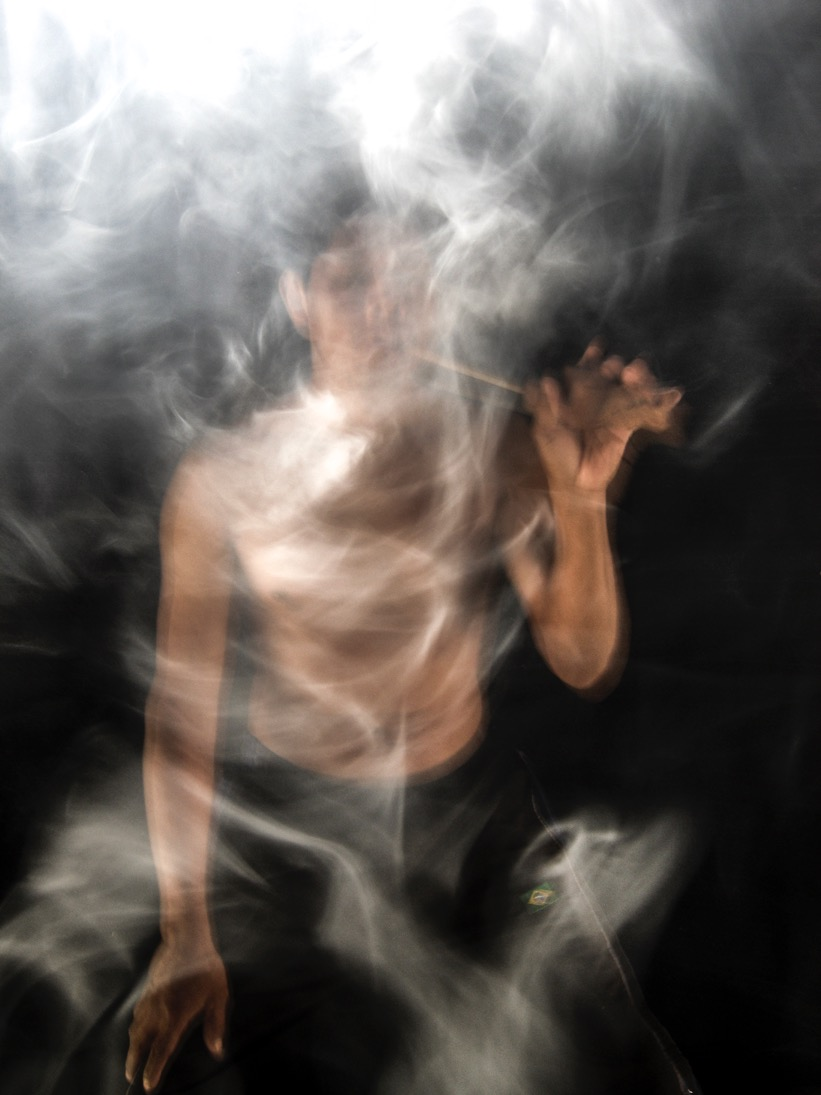
\includegraphics[width=166mm]{./img/GUARANIS-img3.jpg}	
  \hfill
 \end{adjustwidth}
  \caption{Rapaz \emph{mbya} envolto na fumaça do \emph{petỹgua} (cachimbo). Foto: Renilson
Mirim Macena, 2012.}

\thispagestyle{empty}

\end{figure}
\end{vplace}

\end{absolutelynopagebreak}

\makeatletter\@openrightfalse
\movetooddpage
\part{Caminhos e conhecimentos}


%\thispagestyle{empty}

\chapter*{Sonhos e conhecimentos na vida guarani\\
%\bigskip
\large{\emph{Uma experiência de pesquisa na universidade}}}

\addcontentsline{toc}{chapter}{Sonhos e conhecimentos na vida guarani,
\scriptsize{\emph{por Karai Mirim (Algemiro da Silva)}}}

\@openrighttrue\makeatother
\begin{flushright}
\emph{Karai Mirim (Algemiro da Silva)\footnote{Professor na aldeia Brakui,
Angra dos Reis/\versal{RJ}.}}
\end{flushright} 

\noindent
Eu sou Karai Mirim\footnote{Este texto resulta da transcrição e edição
de duas falas de Karai Mirim durante o simpósio ``\versal{CE}st\versal{A} nas Redes
Guarani'', em 16 e 17/10/2013, acrescido de pequenos trechos de seu
Trabalho de Conclusão de Curso na Universidade Federal Rural do Rio de
Janeiro (Nota das organizadoras).}. Infelizmente também tenho nome
português, Algemiro. Como nomeado pelos antropólogos, sou Guarani Mbya,
e sou professor na aldeia Brakui, também chamada Sapukai. Nunca deixei
a aldeia, mas continuo estudando. Como um professor que foi formado na
Sociologia, acho muito importante fazer sempre intercâmbio com os
Guarani e com os \emph{jurua}.

O~pensamento guarani foi negado pelos \emph{jurua} ao longo do tempo. A~gente
achava que o conhecimento dentro da comunidade, nossa vivência, não
significava nada para os \emph{jurua}. Mas a partir do momento que fui
estudando, minha pesquisa modificou muito esse pensamento. Minha
pesquisa me ajudou a pensar e a repensar a nossa cultura. É~importante
fazer intercâmbio porque existem várias aldeias, cada uma com sua
formação, cada professor guarani também tem sua formação diferente.
Então é importante trazer o intercâmbio entre os Guarani também, pra
reunir o nosso conhecimento. Sabemos que os Guarani se espalharam pelo
Brasil, pelo continente, e então cada conhecimento tem sua história.
Com esse encontro, nosso conhecimento talvez possa ajudar a sociedade
não indígena e a gente a viver melhor.

Isso que eu escrevi, não escrevi ontem, não escrevi hoje, não. Venho
escrevendo há anos. Na verdade, é uma pesquisa, como vocês chamam. Eu
fiz o curso de Licenciatura em Educação do Campo na Universidade
Federal Rural do Rio de Janeiro, e aprendi que para os \emph{jurua} é
importante escrever. Eu não pensei que era assim, para mim a
universidade era para participar e receber papel para eu dar aula na
comunidade. Mas cheguei lá e era diferente, tem que participar, tem que
fazer prova, tem que escrever\ldots{} Era muito difícil porque o Guarani é
mais de falar do que de escrever. Como botar o pensamento guarani no
papel? Na linguagem guarani tem a língua que é usada diariamente e a
linguagem que é usada dentro da \emph{opy}, que é muito difícil para traduzir.

Vivo na aldeia Brakui, hoje chamada também Sapukai, em Angra dos Reis,
no Rio de Janeiro. Nunca saí da aldeia, desde criança, só saí para
estudar. A~universidade manda fazer monografia, então eu tive que me
esforçar muito para botar no papel meu pensamento e o pensamento da
comunidade. Foi difícil. Eu moro na aldeia, tenho relações muito boas
com a comunidade, mas percebi que pra fazer pesquisa e perguntar para
as pessoas do modo que a Universidade faz, tendo que gravar, foi
diferente.

No nosso jeito de ser, não é qualquer hora que podemos chegar e
pesquisar. Não é assim que funciona com os Guarani. Tudo tem seu tempo,
como fala Vera Mirim, meu pai. Com ele demorei dois meses somente para
falar sobre o assunto da pesquisa. Para iniciar a nossa conversa,
sempre perguntava o que ele tinha sonhado na noite passada. Então eu
conversava sobre outros assuntos, mas não era mais a pesquisa. Era uma
conversa sobre remédios, histórias, piadas. Ele é muito brincalhão,
nossas conversas eram animadas e ríamos bastante. Só muito depois que
gravei uma entrevista. 

Após a perda de pessoas importantes de sua vida, Vera Mirim começou a
sonhar, \emph{oexa ra’u}. Vários Guarani já me contaram que os sonhos se
intensificaram a partir de acontecimentos trágicos, tristes. Com Vera
Mirim aconteceu o mesmo. Para você ser um bom sonhador, é preciso viver
de acordo com \emph{teko~ete’i}: rezar bastante, participar de todas as
cerimônias, tem que ir à \emph{opy}, se dedicar o máximo possível.

Eu escrevi sobre aldeia e sobre o sonho, como que os Guarani acham o
lugar para morar ou fazer \emph{tekoa} a partir do sonho. Um colega meu que
era mais velho, infelizmente já falecido, quando a gente morava lá em
Paranaguá (\versal{PR}), ele me contou assim: ``Ah, ontem eu fui lá pro Brakui''.
Eu dei risada, todo mundo deu risada. ``Como assim foi lá?''. Ele falou:
``Fui lá, andei por lá, tem cachoeira, tem água, só que não tem peixe'',
e no final ele contou que tinha sonhado isso. Lembrando dessa história,
perguntei para o meu pai o que ele tinha sonhado para chegar na aldeia
de Brakui. Aí ele falou que quando tinha 13 anos ele já sonhava com o
lugar. Mas no sonho não se vê exatamente igual. Ele sonhou, mas não
sabia exatamente onde era. Depois do sonho, passou um tempo, muito
tempo depois, era no final de 1989, e ele foi lá pra Brakui e viu tudo
aquilo que ele sonhou. Então tudo tem essa relação com o sonho.

Tem dois tipos de sonho: o da revelação e o que é exatamente o sonho
mesmo, \emph{oexa ra’u}. Pra gente \emph{oexa} é ver, \emph{oexa ra’u} é ver, mas não ver,
ver de olhos fechados. \emph{Oexa ra’u} o lugar, e para conseguir escolher o
lugar, tem que ter mel que os deuses deixaram pra nós. Quando tem isso,
já dá pra morar. E~aí água, montanhas, animais específicos tem que ter
pra gente poder morar. Então escrevi sobre isso que meu pai falou. Para
fazer aldeia tem que ter um lugar considerado \emph{ka’aguy mirῖ}. \emph{Mirῖ} pode ser
entendido por ``pequeno'', mas tem outra dimensão, que é ``sagrado''.
Lá na Universidade me pediram para eu explicar o que é um local de \emph{ka’aguy
mirῖ}. Eu falei pra eles que \emph{ka’aguy mirῖ} é o guarani que considera sagrado, não dá pra descrever, pra mostrar a partir de certas coisas.
Pra quem não conhece não é nada, é só um lugar.

\section{Os sabedores na aldeia}

Para estruturar a aldeia, tem que ter um sábio que dá nome para as
crianças, para os Guarani, e tem que ter parteira. Porque não tendo
parteira, não vai nascer criança. E~nascendo criança, depois de um ano,
tem que receber o nome guarani. E~o que falta mais? Tem que ter
conhecedor de remédio. O~próprio Vera Mirim (ou João da Silva), meu
pai, falou sobre isso, que tendo essas três pessoas, três sábios, se
consegue estruturar a aldeia: o que dá nome, a parteira e o que faz
remédio.

É~muito importante o papel da parteira na aldeia, porque a hora do parto
é sagrada, é uma cerimônia, pra nós não é um parto normal. O~pai da
criança deve estar presente e preparar uma estira de taquara para
cortar o cordão umbilical. Também deve enterrar a placenta da criança
dentro da casa.

Tem cinco parteiras lá na aldeia, e eu escolhi uma pra entrevistar. Eu
sei algumas coisas que meu pai me ensinou e a partir daí eu fiz as
perguntas. Elas falam que é muito difícil agora devido ao \emph{jurua}, os
brancos. Quando a criança nasce dentro do hospital não tem mais
cerimônia, então é muito triste. Quando fiz entrevista, as mulheres
falaram que deveria ter diálogo do doutor com a parteira. 

Eu falo também na pesquisa do \emph{ipoporã}, que traduzindo literalmente é
``mão bonita'', porque ele tem bastante conhecimento sobre ervas
medicinais. Eu tenho esse conhecimento e na aldeia vários têm, mas eu
não vou dizer que sou \emph{ipoporã}. Também pajé não fala que é pajé. Nós,
vamos dizer, ``usuários'', que dizemos que ``ele é pajé''.

O~José, conhecido por todos os Guarani como Karaja’i, ele sabe remédio
para curar doença, para arranjar namorado, namorada, muitas coisas. Eu
perguntei pra ele se podia resgatar a história e ele disse que podia,
mas não permitiu tirar foto das plantas. Então eu disse ``tudo bem, não
é pra tirar mesmo, mas só pra dizer que tem conhecimento''. Aí ele
concordou em falar e comentou também um pouco do sonho. Desde o
primeiro momento da criação do mundo os Guarani viviam no sonho. Mas é
muito preocupante que hoje em dia estamos sonhando outras coisas. Eu
espero que os Guarani sempre sonhem. Guarani sonha geralmente com
animaizinhos quando vão ter filho. Primeiro sonha e depois confirma. Se
for filho homem sonha com animaizinhos maiores, geralmente com caititu.
E~quando tiver filha sonha com ave. Esse sonho com os animaizinhos são
\emph{nhe’ẽ}. Vera Mirim fala ~assim: ~``\emph{Nhe’ẽ porã}'', ~porque ~não ~é
~qualquer ~espírito. Até hoje, quando sonha com peixe, o sonho é
realizado na comunidade. Quando sonha com mel é gripe. Fogo é gripe
mais grave. Cobra é sinal que alguém está com raiva de você. Eu escrevi
sobre isso na Universidade.

Quando souberam que fui formado na Universidade, Sociologia, todo mundo
perguntava e me abraçava. Com isso, todos ficaram muito animados em
estudar. Mas a minha preocupação é que os Guarani estudem e voltem pra
aldeia. Tem que sonhar da vida guarani, minha preocupação é isso.
Estudar pode estudar, mas viver sempre em Guarani, sonhar em Guarani.

Para fazer a pesquisa me senti diferente porque no dia"-a"-dia da minha
vida eu converso muito, brinco muito, conto piadas, conto as histórias
dos antigos, conto história de namoro, várias histórias. Mas escrever
sobre os sonhos, que foi meu tema de pesquisa, foi difícil. Mudou meu
jeito de sonhar. Depois de estudar quatro anos na Universidade, eu
sonhava com carro, sonhava que estava na sala de aula, fazendo prova\ldots{}
Quando sonhei com carro, pensei que ia ganhar alguma coisa, mas nada.
Daí eu pensei que todo mundo na comunidade estava sonhando alguma coisa
que não era guarani, e na verdade era só eu que não estava sonhando com
as aldeias. Só meu sonho que foi mudando.

Apesar da tecnologia, da televisão, pelo menos na minha aldeia a casa de
reza está lá, não fica abandonada. Ela fica no centro da aldeia e é
sempre frequentada, tem criançada no pátio, tem um grupo de jovens. Os
Guarani precisam de um \emph{karai} pra dirigir a \emph{opy}, a casa de rezas, mas
meu pai não frequenta muito desde que minha mãe foi embora pro céu e
ele ficou sozinho. Então os jovens entram sozinhos, dançam, rezam. Mas
eu agradeço meu pai, ele brinca muito, ele tem cem anos de idade e diz
que quer namorar ainda, isso é muito legal\footnote{Vera Mirim faleceu
em 2016, posteriormente à redação deste texto.}.

Na minha pesquisa também escrevi que desde o primeiro momento, na
criação do mundo, ou na história, a gente fala muito da religião
guarani. Mas dentro da religião guarani a gente não fala só da
religião. Tem muitos momentos festivos, eu escutava muitas histórias
antigas, de uma casa de reza bem grande\ldots{} Na casa de reza não podia
namorar, se entrava com a namorada e cada um sentava em um canto. Até
hoje a família fala para os jovens: ``vai com o namorado, mas um senta
aqui e outro lá, aqui dentro da casa de reza não pode namorar''.

\emph{Nhandereko ete’i} é o jeito do guarani, mas também se fala na \emph{opy} do
\emph{nhandereko marã e’ỹ}, da vida dos imortais. Só que não é qualquer
pessoa que vai seguir \emph{nhandereko marã e’ỹ} , é muito difícil, é
complicado. E~aí eu me lembro do filme que eu assisti, ``Bicicletas de
\emph{Nhanderu}''. Nós Guarani somos guiados como uma bicicleta, mas não é
qualquer um que é bicicleta. A~vida não é só na casa de reza. Tem tempo
de namoro, tempo de casamento, tem tempo de alegria. É~isso o que
acontece até hoje.

\clearpage

\vspace*{\fill}

\begin{flushright}
\begin{minipage}[c]{0.85\textwidth}
\raggedleft
\footnotesize
\emph{As pessoas se fazem em redes, por saberes que são enredados e pelo
investimento em caminhos de percepção. A~capacidade de concentração que
muitos mencionaram é um modo ameríndio de formular a capacidade de
buscar conhecimento e de não se perder em outros caminhos. Importante
ter sido colocada a questão de que os mais velhos sabem mais. Eles têm
condições de concentração muito grandes e, eu imagino assim, estão
transbordando de capacidade de passar conhecimentos. Isso mostra que o
conhecimento não é uma coisa a se enfiar na cabeça, e sim uma
disposição. Como mudar a escola para que isso possa ser aceito? Como
mudar a escola para se abrir para outras práticas de conhecimento? Isso
é uma questão absolutamente difícil.}

\smallskip
\hspace*{\fill}--- Dominique Tilkin Gallois
\end{minipage}
\end{flushright}

\thispagestyle{empty}

\chapter*{Os \emph{xondaro} e a circulação de saberes\\ no mundo de hoje}

\addcontentsline{toc}{chapter}{Os \emph{xondaro} e a circulação de saberes no mundo de hoje,
\scriptsize{\emph{por Jera Poty Mirῖ (Giselda Pires de Lima)}}}

\begin{flushright}
\emph{Jera Poty Mirῖ (Giselda Pires de Lima)\footnote{Professora na escola da aldeia Tenonde Porã, São Paulo /\versal{SP}.}}
\end{flushright}  

\noindent
Começo dizendo que, mesmo sendo Guarani, mesmo tendo nascido numa aldeia
Guarani"-Mbya, mesmo fazendo parte desse povo que tem conhecimentos tão
belos, tão fortes, ainda diria que eu sei pouco. Todos os dias, o tempo
inteiro eu aprendo muito com os \emph{xeramõi}, com as \emph{xejaryi}, que são as
pessoas mais velhas, mesmo que não sejam líderes espirituais. De fato,
aqueles que têm mais idade sempre sabem mais e eu fico muito feliz de
estar constantemente aprendendo na aldeia. Aí eu passo um pouquinho
desses conhecimentos para os amigos que não são Guarani.

Os mais velhos sabem bastante, e eles mesmos trocam também seus saberes,
já que tem muitos pontos ou situações dentro de um saber que são
diferentes. Mas aqueles que aprendem todos os dias são as crianças e os
jovens. Posso falar só pelas aldeias que eu conheço mais, como a aldeia
do Silveira, no litoral, onde eu vou bastante e gosto muito. Também
pela aldeia de Krukutu, pela aldeia do Jaraguá, que também são da
capital de São Paulo, como a minha aldeia.

Eu nasci e estou há 31 anos na aldeia Tenonde Porã. Ali muita coisa
mudou nos últimos quinze ou vinte anos. Quando eu era criança não tinha
luz na aldeia, não tinha \versal{TV}, só alguns tinham radinho de pilha, mas
para comprar pilha tinham que estar com os \emph{jurua}, e a maioria não
topava muito. A~relação com os \emph{jurua} era muito distante. Nessa época,
era muito mais rápido aprender as coisas da aldeia, o que a gente tinha
que fazer como crianças, ou como jovens, ou como pessoas passando pelo
ritual de passagem pra se tornar adultos. A~gente tinha uma atenção
muito maior para os nossos velhos, para as nossas mães, para os nossos
pais, porque não tinha tantas outras influências.

Eu, quando ainda não era mocinha, esperava que isso acontecesse comigo
porque teria toda a família voltada pra mim: a minha irmã mais velha,
minha tia, minha mãe, minha avó. Todas elas se voltariam pra mim pra me
ensinar melhor como cozinhar, lavar roupa, costurar, cuidar de outras
crianças\ldots{} Também era um momento de aprender muitas outras coisas.
Nessa fase de dez, doze, treze anos, catorze anos, a gente está num
momento de muita curiosidade. A~ideia de saber que muitas pessoas
velhinhas iam ensinar muitas outras coisas era muito esperado.

No mundo de hoje, na Tenonde"-Porã e em algumas outras aldeias que eu
conheço, eu acho que esse conhecimento ainda está muito forte, mesmo
quando está meio que dormindo\ldots{} De fato, hoje tem uma grande
influência do mundo do \emph{jurua} por conta da energia elétrica e da
tecnologia. No mundo guarani também isso está ficando muito mais forte.
Todo mundo tem acesso à internet, acesso à escola, e cada vez mais os
jovens e as crianças ficam muito presos nessa forma de saber. A~gente
pode pensar: ``as crianças e jovens estão muito presos na internet, no
celular, na escola, mas tem os adultos que sabem da cultura, que
dominam a língua e os princípios guarani, então esses não vão deixar a
peteca cair''. Só que às vezes pais e mães, muitos \emph{xeramõi} infelizmente
também ficam assistindo \versal{TV} em casa. Por que o filho, se for
assalariado, comprou uma \versal{TV} de plasma muito bonita, que tem uma imagem
muito de outro mundo, e aí gostam também de assistir filmes de ação,
como o filme do ``Avatar'', que tem efeitos especiais. Os mais velhos
também ficam muito encantados com isso e às vezes deixam de fazer a
roda de história com esses que já vivem num mundo muito cheio de
influências tecnológicas. 

Vou tentar contar alguns pontos mais fortes dessa experiência de ser
Jera, de ser moradora da aldeia Tenonde"-Porã, de ter nascido nessa
cultura, de trabalhar na área da educação, dentro da pouca experiência
que tenho de trabalhar como educadora, mas de sempre ter pensado em como
fazer com que a escola não interferisse de maneira muito agressiva na
educação tradicional. Todas as vezes que me envolvi em projetos pra
fortalecer nossa cultura, que veio se prejudicando por conta da pouca
terra e de não ter mata em muitas aldeias, se envolveram comigo muitos
jovens e crianças, e alguns pais. Talvez os adultos se envolvam menos
porque eles já sabem bastante, mesmo que já não façam atividades de
caça, de pesca, já que não tem como fazer na área. Eles não fazem
porque não tem como fazer, mas sabem.

O~fato é que quando você chama as pessoas pra uma conversa voltada para
esse tema de fortalecer a cultura guarani, a maioria é sempre de
crianças e jovens. Às vezes os mais velhos falam para os novos: ``vocês
não querem mais comer fubá, vocês não querem mais comer milho, vocês
não querem mais comer \emph{mbyta}, \emph{rora}, que são as comidas tradicionais''. O
problema é que quando eles têm seis, sete aninhos, não são eles que vão
para o mercado de \emph{jurua}, são os pais. Então o que o filho sabe comer
hoje foi o pai e a mãe que ensinou. Não adianta o menino fazer quinze
anos e quererem enfiar goela abaixo um \emph{mbyta} (comida feita de milho)\ldots{}

\section{O~despertar dos \emph{xondaro}}

Mesmo quando o sentido de ser guarani, o espírito, a alma de ser guarani
está um pouco dormindo, quando é chamado ele acorda muito rápido. A
gente começou um projeto de fortalecimento do \emph{xondaro} na Tenonde"-Porã
em 2010, quando ele estava muito, muito adormecido. \emph{Xondaro}, que são os
guardiões, era uma coisa que sempre me emocionava bastante quando eu
era criança. Quando os \emph{xondaro} dançavam, eu ficava sentadinha e
sentindo o chão embaixo de mim tremendo. Era uma vibração muito forte,
uma coisa linda, magnífica. Os homens dançam com muita seriedade porque
faz parte do mundo espiritual guarani, que tem uma concepção muito
ampla, grandiosa.

Depois eu fui crescendo e a dança do \emph{xondaro} foi se enfraquecendo na
aldeia. Eu falava para os meus parentes da Tenonde Porã que a gente
precisava fortalecer, trazer de volta o \emph{xondaro} que estava dormindo. O
\emph{xondaro} está muito voltado para o contexto espiritual, de ter seu valor
como Guarani, mas também é uma prática de dança que mexe muito com a
força física. Algumas lutas, por exemplo o karatê, têm movimentos em
que você tem que ficar com os músculos muito tensos pra você atacar
bem, pra você derrubar o seu inimigo. Já no \emph{xondaro} é ensinado a ter a
leveza no corpo. Eu posso jogar alguém a quilômetros de distância com a
leveza do meu corpo, mesmo que a pessoa esteja enrijecida, na
defensiva.

Ser \emph{xondaro} ou \emph{xondaria} não significa só circular, dançar, pular e
rodar\ldots{} Significa você incorporar o espírito guarani e, a partir daí,
saber o que você pode fazer e o que não pode, se você é \emph{xondaro} ou
\emph{xondaria} de quem, de quem você tem que cuidar dentro da sua aldeia e
como você tem que cuidar. Também saber como vão ser seus passos no
futuro, dentro da comunidade que você vive, pra que você seja o \emph{xondaro}
que você tenta ser quando você entra no círculo da dança. A~beleza do
\emph{xondaro}, toda sua concepção, você só entende se você for na aldeia e
ver algumas danças, ou se você dançar.

Quando começamos o projeto, lembro que nas primeiras tentativas de
dança, de levar as crianças e os jovens pra casa de reza, estava todo
mundo meio endurecido. Mas com o começo do projeto foi muito rápida a
desenvoltura do corpo, o retorno do espírito dos \emph{xondaro}, mesmo para
aqueles que sabem pouco da concepção profunda do \emph{xondaro}, como os
pequeninhos de três, quatro anos, que eram todos meio durinhos e agora
fazem coisas lindas, muito fortes. 

Um dos mestres \emph{xondaro}, Pedro Vicente, falou muito para os jovens como é
que as pessoas têm que ser pra aprenderem de verdade o \emph{xondaro}. Com as
palavras de Pedro Vicente, muitos jovens mudaram o comportamento e
começaram a pensar diferente sobre a situação de estarem muito presos a
um mundo que não faz parte da sua cultura. A~Tenonde Porã tem 26
hectares, não tem natureza, não tem como ter contato com animais, com
água, com pesca, com caça\ldots{} então pesa mais a influência tecnológica
do \emph{jurua}, da energia elétrica. Para alguns homens guarani, quando não
tem o que pescar, não tem o que caçar e não tem como entrar na mata e
cortar árvores pra fazer suas casas, também às vezes não tem por que ir
pra casa de reza, pra fortalecer aquilo que não está muito saudável.

Por isso, no projeto a gente contou com lideranças e amigos de outras
aldeias que têm seus espaços maiores, que têm mais natureza, como na
aldeia do Silveira. Então aconteceram coisas lindas, a gente se
fortaleceu, e os jovens da Tenonde"-Porã se fortalecerem enquanto
\emph{xondaro}. Depois a gente também teve a oportunidade de levar os \emph{xondaro}
da Tenonde Porã que já estavam animados, que já estavam acordados, pra
outras aldeias em que esse conhecimento estava também um pouco
dormindo. Mesmo estando em aldeias diferentes, a gente é um povo só e
se entende bastante nesse sentido.

Cada mestre \emph{xondaro} tem suas particularidades, sua concentração, sua
leveza corporal. Quando entram na roda, cada \emph{xondaro} e \emph{xondaria} têm que
ir com seriedade, porque estão dançando também pros \emph{Nhanderu kuery}, para
os nossos deuses, pra gente se fortalecer. Então você nunca pode entrar
rindo. O~\emph{Karai Xondaro}, lá na aldeia do Silveira, parava na frente dos
\emph{xondaro} que não estavam concentrados e ficava olhando, sem falar nada,
até que eles percebecem e parassem de rir ou de falar. Isso acontecia
de uma maneira muito bonita. Esse \emph{Karai Xondaro} tem uma concentração
total, que não é enrijecida. Ele tinha uma \emph{yvyra raimbe}, que é uma
madeira comprida, e fazia muito forte a dança do \emph{xondaro}. Ele passava a
madeira muito rápido para os meninos se esquivarem e eu pensava que
eles iam ser atingidos. Em muitos momentos eu senti meu coração ficar
bem duro, porque parecia que ele ia atingir esses \emph{xondaro} que estavam
dançando com ele e que estavam ainda aprendendo, pois era o começo do
projeto. Eu percebia o medo no rosto do meu sobrinho. Eu queria salvar
todo mundo que estava lá, mas pensei: ``não, esse \emph{xondaro ruvixa} sabe o
que está fazendo, não vai atingir, vai ficar tudo bem''. Então aconteceu
uma coisa linda, porque todos esses \emph{xondaro} que estavam dançando com
eles incorporaram, definitivamente, o espírito dos \emph{xondaro} guarani,
passaram a se concentrar mesmo.

A~gente teve há pouco tempo movimentos muito fortes que vieram a partir
desses \emph{xondaro} que foram acordados. Mesmo quando os \emph{xondaro} não estão
dançando, não estão ativos na aldeia, os Guarani em todas as situações
de precisão um do outro se unem, a gente senta junto, conversa junto, a
gente vai junto. Nos últimos dois anos eu senti muito forte o movimento
dos \emph{xondaro} em vários cantos dos territórios guarani ficar mais forte.
Cada vez fica mais forte os \emph{xondaro} se sentirem \emph{xondaro} na situação de
cuidarem um do outro e, a partir disso, quererem fazer as coisas sem
descanso. Está acontecendo um movimento espiritual também de fazer as
coisas acontecerem e de se cuidar na aldeia. Quando tem problema, por
exemplo, de bebida alcoólica na aldeia, os rapazes dizem: ``você tem que
beber menos, você é \emph{xondaro}! Você não pode fazer isso. Assim não dá!''.
Eles têm essa cobrança um com o outro, e também de quererem fazer as
coisas como eu disse antes, sem dormir, por muito mais tempo, pra
acordar.

Isso tudo está ligado aos movimentos indígenas quanto às questões das
terras, da demarcação das terras. Teve o primeiro movimento que
aconteceu na rodovia dos Bandeirantes, que a gente fechou pra protestar
contra a demora nas demarcações, perto da aldeia de Jaraguá. Depois a
passeata na Avenida Paulista, que era pelas demarcações e contra a \versal{PEC}
215. Na Tenonde"-Porã e na Krukutu, a gente também está fazendo um
movimento de retomada de nossas terras de ocupação tradicional. Há seis
dias a gente retomou a aldeia Kalipety, que era habitada por nosso povo
na década de 70. Eu queria estar fazendo essa conversa que eu estou
fazendo com vocês lá. Se eu pudesse transportar todo mundo pra lá seria
bom, só pra vocês sentirem isso como eu estou sentindo.

Nesses seis dias, há momentos em que a gente foi ficando cansado,
fisicamente. A~gente ia desanimando, mas aí o \emph{xeramõi} punha a mão na
nossa cabeça e falava ``\emph{nembaraete katu}'', que é uma forma de nos
alimentar espiritualmente. Aí ficava todo mundo muito animado de novo!
``Bora fazer casa!'', ``Bora lá, então!''. 

Esse é um começo, a gente ainda está ganhando experiência. Mas a
retomada de terras tradicionais é muito marcante para o povo guarani.
Se algumas práticas da cultura guarani estavam dormindo, mas
conseguiram acordar mesmo em áreas que não tem natureza, imagina o que
pode acontecer numa área ampla e que tenha água, que tenha cachoeira,
que tenha o que caçar? Ontem mesmo eu estava falando para os meninos:
``imagina aqui quando vocês matarem uma caça de grande porte e a gente
puder distribuir pra todo mundo?''. Não vou repetir as palavras que eles
falaram, mas ficaram bem empolgados!
%no original está 'e a gente poder' Seria o caso de manter o erro, uma vez que se trata da transcrição de uma fala?

\section{A~escola e os saberes}

A~maioria de projetos que eu escrevo para fazer na aldeia é de
``transmissão de saberes'', mas estou gostando mais da ideia de
``circulação''. Nessa circulação de ações voltadas para o aprendizado
informal, diferenciado, tradicional, o que me preocupa bastante é esse
modelo da educação que a gente tem hoje dentro das aldeias
Guarani"-Mbya. Esse modelo nasceu da Constituição, que assegura o
direito da criança indígena a ter uma educação diferenciada, tanto
dentro do mundo da sociedade envolvente como no mundo tradicional. Mas
para os Guarani"-Mbya a educação diferenciada é muito recente.

O~povo Guarani foi um dos primeiros povos a ter contato com os \emph{jurua}. E
ainda assim, em aldeias como a Tenonde Porã, o Silveira, Krukutu,
aldeias muito próximas da cidade, muito próximo de toda a influência do
\emph{jurua}, ainda têm pessoas que não sabem falar o português, que se mantêm
muito no mundo Guarani. Diante disso, quando a escola entrou na aldeia,
os que estão muito no mundo dos Guarani não estavam dispostos a
conversar sobre qual tipo de educação que a gente vai fazer na escola.
O~que se tinha era uma coisa muito superficial, de que a gente precisa
aprender a falar a língua do \emph{jurua} pra saber lidar melhor com as coisas
do \emph{jurua} que chegam na aldeia. 

No início, quando eu tinha doze ou treze anos, eu lembro bem que a ideia
de aprender a língua ou os conhecimentos \emph{jurua} era pra lutar pelos
direitos, era para coisas específicas\ldots{} Como as pessoas que estavam
indo pra Brasília e que não sabiam falar direito o português, e que
tinham que aprender a escrever e a ler, enfim, ter capacidade de fazer
decodificações de documentos complicados, por exemplo, a fim de não ser
enrolado. Só que aí foi indo, foi indo, foi indo e o que a gente tem
hoje é isso, além de você ter que aprender pra se defender da cultura
do \emph{jurua}, se politizar e conhecer seus direitos, a escola está trazendo
uma ideia de padronização, de que você tem que ir pra escola pra ter um
trabalho, pra ter um dinheiro e aí você pode também ser igual àquele
que tem um carro\ldots{}

A~gente não soube lidar com esse modelo de escola quando ele entrou na
aldeia. Ainda hoje não sabemos direito, e há muitos conflitos com
outros professores, com a comunidade, com os representantes das
políticas. Eu tinha pensado como seria bom ter uma semana de escola e
outra sem escola, e fiz essa proposta na última Conferência Estadual de
Educação Indígena. Mas ninguém concordou comigo!

A~escola descaracteriza muito o cotidiano das comunidades guarani.
Quando a criança guarani tem um tempo rígido para ir para escola e tem
que cumprir um horário, aos poucos vai perdendo a delicadeza em
respeitar o seu momento. Por exemplo, as meninas quando estão
menstruadas não devem ir para a escola, mas isso quase nunca é
respeitado.

Antes eu ficava meio depressiva, mas hoje fico feliz porque às vezes o
\emph{jurua} fala eu não entendo tudo. Às vezes quando o Guarani fala eu
também não entendo tudo, e aí eu penso: ``nossa como eu tenho que
aprender ainda!''. E~isso é bom. Às vezes um \emph{xeramõi} está falando na
casa de reza e eu me sinto analfabeta na minha própria língua, não
entendo quase nada do que está sendo dito. O~\emph{xeramõi} Pedro Vicente
tinha dito pra mim que, pra gente ser uma pessoa com dom, pra saber
contar histórias, também tinha que ter \emph{arakuaa}. Ele não falou \emph{arandu},
que é uma palavra usada para ‘conhecimento’, ‘sabedoria’. Ele disse que
aprender a escrever é ter \emph{arandu}, é ser inteligente. Mas o \emph{arakuaa} está
mais voltado para uma questão espiritual, que é uma linguagem mais
voltada e mais usada no mundo da \emph{opy}. Assim, hoje existem vários meios
de conhecimento: tem \emph{xeramõi}, tem Google, tem os livros, os
antropólogos, entre muitos outros\ldots{}

\clearpage

\vspace*{\fill}

\begin{flushright}
\begin{minipage}[c]{0.85\textwidth}
\raggedleft
\footnotesize
\emph{A~palavra \emph{xondaro}, que quer dizer tanta coisa, para os Guarani Mbya é
como que uma metáfora da relação de uma pessoa que está conduzindo o
processo e dos auxiliares que estão dispostos a levar esse processo
adiante. Isso me leva à questão da relação das divindades concebidas
como os irmãos mais velhos dos homens. O~pai do seu Algemiro me contou
que quando o primeiro \emph{Nhanderu} criou o irmão, ele criou uma cópia
transformada de si mesmo. E~daí eu fiquei pensando no processo de
educação como o imitar, como a criança está sempre imitando os adultos
e a partir disso estão aprendendo. Só que estão imitando e
transformando esse conhecimento. Esses irmãos mais velhos são o modelo,
mas não necessariamente um modelo fixo. É~preciso sempre estar
experimentando, porque imitar é sempre transformar.}

\smallskip
\hspace*{\fill}--- Daniel Calazans Pierri
\end{minipage}
\end{flushright}

\thispagestyle{empty}

\chapter*{Processos de aprendizado\\ pelos olhos das crianças guarani mbya}

\addcontentsline{toc}{chapter}{Processos de aprendizado pelos olhos das crianças guarani mbya,
\scriptsize{\emph{por Alice Haibara}}}

\begin{flushright}
\emph{Alice Haibara}\footnote{Doutora em antropologia pela \versal{USP} e membro do
\versal{CE}st\versal{A}.}
\end{flushright}

\noindent
O~objetivo deste texto é refletir sobre como se dão os processos de
aprendizado entre as crianças guarani mbya, analisando principalmente o
contexto da aldeia Tenonde Porã, que fica localizada na região sul da
cidade de São Paulo\footnote{Este artigo é baseado em uma pesquisa de
iniciação científica, realizada durante o período de graduação entre os
anos de 2010 e 2011, pelo Departamento de Antropologia \versal{USP}, com
orientação de Dominique Tilkin Gallois. As análises e os dados aqui
apresentados foram produzidos em colaboração com a professora Jera
Guarani, a quem agradeço imensamente.}. A~partir da observação de
diferentes contextos, pretende"-se evidenciar alguns aspectos dos
diversos modos de construção e circulação de saberes entre os Guarani,
para então refletir sobre como estes modos próprios de conhecer se
relacionam com as formas de aprendizado características da escola.

Os pressupostos da pesquisa se baseiam numa atual Antropologia da
Criança, em que as crianças são vistas como participantes ativas de
seus processos de aprendizado e não como um mero receptáculo de
informações (Cohn, 2000). Desta forma as crianças são compreendidas com
base na construção de um universo que lhes é próprio, considerando que
elas possuem conhecimentos qualitativa e não quantitativamente
diferenciados do mundo adulto (idem, 2000). Quando buscamos entender as
crianças e seu contexto social a partir do ponto de vista delas mesmas,
é possível construir uma apreensão que é diferenciada e relevante,
sendo possível muitas vezes evidenciar aspectos sociais que não são
explícitos (Toren, 1993). Neste sentido, buscamos ouvir e dar
visibilidade ao que as crianças guarani pensam, como concebem o mundo
em que vivem, como compreendem a si mesmas, seus corpos, suas
expressões, seus aprendizados e experiências. 

\section{As \emph{kyringue} guarani mbya}
Entre os Guarani, as crianças têm um lugar de grande importância. De
acordo com alguns interlocutores, a partir do momento em que diminuírem
ou acabarem as crianças, \emph{Nhanderu} (Nosso Pai) acabará com a vida na
Terra. Jera Guarani (2008: 39) afirma que:

\begin{quote}
\noindent
O~povo Guarani compreende que o espírito da criança é enviado por
\emph{Nhanderu} (\ldots{}) sempre com uma missão: às vezes para fortalecer o pai, a
mãe, ou até mesmo os avós, e em algumas situações para fortalecer o bem
estar da união entre o casal. Por isso a criança era recebida com muito
amor e carinho e, acima de tudo, com muito respeito, pois para os
Guarani o espírito se liberta desta vivência humana para a morada
sagrada de \emph{Nhanderu} e volta como criança, muitas vezes com o mesmo tipo
físico, ou alguma outra característica do que já fora um adulto ou um
velhinho, em vidas passadas. A~criança representa para o povo Guarani a
vontade do Criador, em dar continuidade à vida para o nosso planeta.
\end{quote}

Existem diversas práticas e cuidados feitos na ocasião do nascimento de
uma criança, desde o momento da gestação até o período do pós"-parto.
Tais práticas visam à formação da pessoa, de maneira que os processos
atravessados pelo espírito se relacionam diretamente às ações de
fabricação do corpo. Dentre diferentes medidas podemos citar algumas,
como quando a mãe faz um pequeno colar com o cordão umbilical do bebê e
deixa pendurado em seu pescoço até que ele seque, ou a prática do pai
enterrar a placenta em um buraco dentro da casa. Ambas atitudes visam
fazer com que a criança tenha um espírito assentado e se torne uma
pessoa concentrada (Lima, 2008).

Entre as concepções e práticas guarani é notório perceber que o espírito
da criança está intimamente relacionado ao pai e as suas ações. De
acordo com Jera Guarani, durante os primeiros seis ou sete meses de
vida da criança, o homem deve continuar seus afazeres, mas seguindo um
ritmo mais baixo, não realizando atividades bruscas, como carpir ou
cortar coisas. Por exemplo, se ele cortar uma árvore, esta poderá cair
sobre o espírito da criança e a mesma ficará doente. Também não se deve
jogar futebol, pois como o espírito do filho passa o tempo todo com o
pai, e se este ficar correndo para lá e para cá, a criança vai se
cansar muito, uma vez que seu espírito vai tentar fazer todas as
atividades que o pai está fazendo. Quando isso ocorre os Guarani dizem
que a criança está \emph{harua} (cansada e sentindo incômodos ou cólicas), e
as pessoas costumam afirmar: ``Seu filho está \emph{harua}, você fica tendo
comportamentos errados!''. Também a presença do pai próximo ao filho se
faz muito importante, de modo que o homem ``não deve se ausentar por
muito tempo, sair ou viajar nos primeiros meses de vida da criança''
(Melo, 2008: 85). Como a alma da criança está fortemente ligada ao pai
depois do parto, ele deve sempre marcar os caminhos que percorre, para
que a alma do seu filho não se perca (Clastres, 1978).

A~importância em fazer com que a alma da criança permaneça forte no
corpo é algo presente nas concepções e nas práticas guarani (assim como
em diversos outros grupos ameríndios). Dessa forma, deve"-se evitar que a
criança chore ou fique triste, pois isso pode fazer com que seu
espírito queira retornar para o lugar celeste de onde veio. Assim, para
alegrar e acalmar os bebês, é ensinado às mães que elas devem caminhar
e cantar os \emph{mitã monguea} (canções de ninar). Já os \emph{mborai ete} (cantos
verdadeiros), realizados durante as cerimônias na \emph{opy} (casa de reza),
não devem ser cantados para os bebês muito pequenos porque são canções
ensinadas e enviadas aos \emph{yvyra’ija} (lideranças espirituais), de modo
que o bebê poderia se recordar da morada sagrada e assim querer
retornar para lá antes de cumprir sua missão.

De acordo com Testa (2008), entre os Guarani há uma ideia frequentemente
afirmada de que ``a vida de cada um é seu caminho de buscar e aprender''.
A~pesquisadora associa o processo de aprendizado à noção de um ``caminho''
a percorrer. Nesse sentido, é possível dizer que desde a ocasião do
nascimento da criança já são realizadas diversas ações para que se
tenha concentração e direcionamento no caminho de vida e aprendizado
(relacionadas ao destino da placenta e cordão umbilical, por exemplo),
e também para facilitar o ``caminhar junto'', quando o pai ``marca os
caminhos'', ou mesmo quando evita realizar atividades em que o espírito
da criança terá dificuldade de acompanhá-lo. Desta forma, é possível
dizer que as ações de ``acompanhar'' os pais e mães imitando as suas
práticas e comportamentos já são realizadas pela pessoa quando ela
ainda está na barriga da mãe. O~mesmo sentido é possível dar às
práticas que visam manter o espírito da criança forte no corpo, pois
assim a pessoa não irá seguir o caminho de retorno à morada de \emph{Nhanderu}
antes do tempo, podendo realizar seu caminho de aprendizado na Terra. 

As ações de fabricação do corpo, relacionadas aos processos do espírito,
mostram que entre os Guarani o conhecimento é construído ``caminhando e
aprendendo junto'', o que pode ser entendido também como um tipo de rede
de relações entre os sujeitos envolvidos na formação da pessoa. Tal
rede se constitui especialmente pelas relações entre os corpos e é por
meio da corporalidade que a pessoa guarani aprende a construir e
direcionar seu caminho. Adentrando no contexto da \emph{opy} (casa de reza), é
possível verificar algumas práticas de ``aprender junto'' realizadas no
corpo e por meio do corpo.

\section{Na \emph{opy}}

Na Aldeia Tenonde Porã, no início da noite, algumas pessoas se reúnem na
\emph{opy}. As mulheres acendem o fogo e esquentam a água para tomar \emph{ka’a}
(erva"-mate). As pessoas sentam"-se em volta da fogueira em bancos e
cadeiras conversando descontraidamente, alguns cobertores são
estendidos no chão, onde se acomodam mulheres com seus filhos. As
crianças pequenas mamam e brincam, dormindo quando sentem vontade. Os
\emph{petyngua} (cachimbo) vão sendo acesos, os homens vão se levantando e
caminham num trajeto circular até o \emph{amba’i} (altar), seguem fumando e
assoprando a fumaça em todo o redor. Algumas crianças fazem o mesmo,
geralmente os meninos e também algumas meninas, embora com menos
frequência. O~som do violão começa a soar e as pessoas se levantam para
cantar e dançar. 

O~papel das crianças na \emph{opy} é muito importante, cantando, dançando e
participando ativamente. Durante algumas conversas, elas demonstraram
ter interessantes compreensões em relação às práticas realizadas neste
contexto, relacionando"-as com os processos de comunicação e interação
com diferentes aspectos da cosmologia guarani. Assim, Kerexu, de dez
anos, explicou o papel do \emph{xeramõi} (liderança espiritual masculina,
traduzido como ``meu avô'') e demonstrou, através de gestos e sons, como
ele realiza as curas, fazendo uso das mãos e da boca, por meio de
sopro, sucção, cantos e do \emph{petyngua}. De acordo com a menina, o \emph{xeramõi}
arrasta a mão nas costas e na barriga da pessoa até formar uma pedrinha
que ele entrega para o \emph{xondaro} (``os guardiões da \emph{opy} e da aldeia'', em
sua definição), que dá para a \emph{xejaryi} (liderança espiritual feminina,
traduzido como ``minha avó'') jogar no fogo. 

Kerexu afirma que esta pedrinha é de \emph{Anhã}, traduzida pela menina pelo
termo ``satanás'', e que é jogada no fogo para que ``\emph{Anhã} pegue de novo a
pedra dele''. Ao falar sobre o processo em que as pessoas ficam doentes
por causa da pedrinha, ela descreve:

\begin{quote}
\noindent
Quando as pessoas rezam muito e são de \emph{Nhanderu}, diz que o \emph{Anhã} fica
muito bravo, e aí quando a gente anda --- minha mãe que me contou --- as
pessoas que já são mortas pegam uma pedra, que não é venenosa, mas tem
maldição, e jogam. Aí é doença de \emph{Anhã} quando a pessoa fica muito mal
mesmo. Sabe quando o \emph{xeramõi} fica ``\emph{argh, argh}'' (sonorização), é que tem
uma pedrinha envenenada que eles tiram da pessoa e jogam no fogo.
\end{quote}

Kerexu afirma saber como o \emph{xeramõi} realiza as curas porque ela mesma já
passou pelo tratamento:

\begin{quote}
\noindent
É~porque ele já tirou uma pedra de mim. Na verdade, eu não estava
sonhando direito, eu dormia muito mal e sonhava muito com coisas ruins.
\end{quote}

Ao ser perguntada sobre o motivo da doença ser retirada das costas, a
menina responde:

\begin{quote}
\noindent
Por que a sombra vem daqui de trás, a gente anda, fica feliz. O~\emph{Anhã}
joga a pedrinha só em quem vai pra \emph{opy}, quem reza mais. Os bêbados ele
deixa ficarem felizes sem doença. Mas da pinga eles ficam doentes.
\end{quote}

Kerexu afirma ainda que quando ficar velhinha quer muito fazer as curas.
A~menina também explicou a função da fumaça e do \emph{petyngua}:

\begin{quote}
\noindent
O~\emph{petyngua} serve só pra \emph{Nhanderu} ouvir. Quando a gente fuma a gente
reza, mas eu não rezo, eu não falo nada pro \emph{Nhanderu}. Só às vezes
quando eu não durmo bem eu falo e também quando eu canto bem alto, no
meu cérebro eu falo, deixa a minha voz mais forte, deixa meu corpo e
minha família fortes, e também pra eu dormir bem.
\end{quote}

As explicações oferecidas pela menina, com base em sua própria vivência
da doença e da cura evidenciam a importância da dimensão corporal em
tais aprendizados. Para explicar como as curas são realizadas, Kerexu
se valeu muitas vezes de demonstrações com as mãos, sopros, com os
quais ela imitava as ações realizadas pelo \emph{xeramõi} na \emph{opy}. A
experiência de já ter sido tratada é algo que certamente foi muito
importante para que ela pudesse relatar com mais profundidade essas
práticas. Seus comentários também enfatizaram a experiência do sonho,
mostrando a importância de dormir bem e os tipos de sonhos em sua
relação com doenças, curas e categorias \emph{Nhanderu} e \emph{Anhã}.

Os sonhos são muito valorizados pelos Guarani, constituindo um
importante modo de saber. Um exemplo disso é que o \emph{xeramõi} pode receber
através dos sonhos os nomes guarani que serão dados aos bebês,
indicando a região celeste de onde vem o espírito daquela pessoa.
Também os cantos realizados na \emph{opy} muitas vezes chegam por meio dos
sonhos, algumas vezes inclusive sonhados por crianças.

Todas as crianças com quem conversamos afirmaram gostar muito de ir à
\emph{opy}, e um dos motivos mais recorrentes apontados por elas é que lá elas
cantam e dançam. Menezes (2004) afirma que a dança é uma importante
ferramenta no processo de educação e formação do corpo e do espírito
guarani. Montardo (2002: 12) também
ressalta a importância dos cantos e das danças no aprendizado guarani e
na formação de seus corpos, afirmando que na dança o corpo é quem
abriga os saberes vivenciados e a música praticada em seus rituais
cotidianos se constitui num ``caminho a percorrer ao encontro dos
deuses'', em que ``os Guarani pretendem, neste caminho realizado no
ritual, embelezar e fortalecer os corpos, dotando"-os de força e de
alegria, combatendo a tristeza''.

As práticas de cantos e danças entre os Guarani também podem demonstrar
um aspecto dos seus modos de aprendizado, que é o gosto em aprender
junto. Neste sentido, cantar e dançar se configuram em atividades que
possibilitam a formação da coletividade no próprio corpo, pois canta"-se
junto, numa só voz, e dança"-se de mãos dadas ao mesmo passo. Há
diferentes tipos de formação nas danças, em alguns casos formam"-se
fileiras em que as pessoas ficam posicionadas umas ao lado das outras,
em linhas retas, viradas de frente para o \emph{amba’i}, os homens
localizam"-se nas fileiras da frente e as mulheres mais atrás. A~dança,
nesse caso, se dá com pequenos movimentos dos pés e pernas que se
levantam e abaixam. Todos seguem os ritmos dos instrumentos e dos
cantos acompanhando o \emph{yvyra’ija}, o qual puxa a cantoria com o violão.
Outra forma de dança é quando as fileiras se organizam em torno do
\emph{amba’i} formando um grande círculo, neste caso as fileiras das mulheres
ficam na parte interior do círculo e os homens ficam atrás, todos de
mãos dadas seguem pulando e se movimentando juntos, em círculo, por um
longo tempo. Esta dança exige uma grande força e resistência,
características que são valorizadas pelos Guarani tanto no sentido
físico como no espiritual.

Certo dia, durante uma reza na Aldeia Tenonde Porã, estavam realizando
esta dança que consiste em pular juntos em círculo. Após pular por
muitos minutos, uma menina de oito anos sentou"-se e disse, ``aquelas
meninas do Silveira são fortes, né?'' (referindo"-se às crianças que
vieram de outra aldeia e estavam participando da reza). Em seguida, ela
parou um pouco, pensou e disse: ``todos nós somos fortes, só não são
fortes aqueles que não ajudam''. Assim temos mais um exemplo da relação
entre o aprendizado corporal da dança e a valorização da força para os
Guarani. Outro ponto que também transparece na fala da menina é a ideia
de que aqueles que ajudam a realizar as atividades na \emph{opy} se tornam
pessoas fortes, em detrimento daqueles que não participam. De forma que
muitas vezes o empenho dedicado a tais atividades vai refletir em quem
será essa pessoa num contexto mais amplo da comunidade. Assim, grande
parte das lideranças na aldeia são pessoas que estão envolvidas no
contexto da \emph{opy}.

Há diferentes atividades que são realizadas em tal contexto, como por
exemplo, picar o fumo, acender os \emph{petyngua}, cuidar do fogo, esfriar a
água para quem termina de fumar, tocar os instrumentos musicais, entre
outras. Cada criança tem espaço para manifestar de forma autônoma as
atividades em que mais se identifica e assim vai desenvolvendo suas
habilidades corporais, assumindo funções e determinando o seu papel na
\emph{opy}. Tal afirmação pode ser relacionada com a fala da menina Kerexu, em
que esta declara que quando está na \emph{opy} gosta de cantar muito alto,
para que todos vejam que ela é uma \emph{xondaria}. Ao descrever o que é ser
\emph{xondaria} ela afirma:

\begin{quote}
\noindent
Ah! \emph{Xondaria} é uma mulher que é boa, uma menina, pode ser uma mulher,
uma menina, uma avó, vovozinha. \emph{Xondaria} quer dizer uma mulher forte
que também é do Conselho\footnote{``O~Conselho'' é uma forma de
organização social e política da comunidade, em que as lideranças se
reúnem para discutir e decidir os assuntos coletivos. }. Mas eu não sou
do Conselho. E~também é uma mulher que canta muito, reza e fuma muito.
\end{quote}

Ao mesmo tempo em que o ato de aprender junto é muito valorizado, o
empenho pessoal de cada um, ao buscar aprender e realizar seu papel,
desenvolvendo as funções com que mais se identifica, torna cada pessoa
única em seu caminho. As crianças neste sentido mostram"-se como seres
autônomos na construção de sua aprendizagem, pois neste contexto agem
de acordo com sua própria vontade, respeitando seu tempo e suas
preferências. No entanto, a figura do \emph{xeramõi} e da \emph{xejaryi}, assim como
de todas as pessoas mais velhas presentes, constitui algo fundamental
que opera na base de funcionamento da \emph{opy}. É~possível observar que as
crianças demonstram um grande desejo de fazer tudo o que os mais velhos
fazem. Quando vão até o \emph{amba’i}, ou fumam \emph{petyngua}, por exemplo, elas
procuram imitar todos os passos dos mais velhos e assim vão aprendendo.
Neste sentido, a imitação ou cópia não é entendida aqui como mera
reprodução e podemos pensá-las como processos que são sempre criativos,
pois toda imitação envolve também improvisação, como formula Tim Ingold
(2010: 21): ``copiar é imitativo, na medida em que ocorre sob
orientação'' e é fruto de improvisação ``na medida em que o conhecimento
que gera é conhecimento que os iniciantes descobrem por si mesmos''.

\section{Aprendizados como relações}

A~\emph{opy} certamente é um importante contexto para o aprendizado. No
entanto, entre os Guarani, existe uma concepção de que o processo de
construção de conhecimentos pode acontecer em diferentes lugares e
momentos. Desta forma, o que importa é a busca pessoal de cada um e as
relações que se constituem em cada contexto. 

Assim, nos momentos em que se encontram em casa, ou nos arredores da
aldeia, as crianças guarani não são chamadas para o aprendizado formal
ou sequencial pelos pais. Elas podem observar, quando querem, as ações
dos adultos, das crianças e de tudo o que há em seu entorno, imitando e
improvisando à sua maneira. É~pela observação, curiosidade e
experimentação que vão trilhando seu próprio caminho. O~processo de
construção de conhecimentos vai acontecendo por meio do desenvolvimento
da percepção, que se constitui ``como uma atividade de todo o organismo
num ambiente'' (Ingold, 2010: 21). O~‘ambiente’ é compreendido aqui,
como algo habitado, que não se restringe apenas ao espaço físico, mas
compõe"-se também por ele. Neste sentido, as relações estabelecidas com o
ambiente se constituem nas relações de aprendizado.

É~possível observar a liberdade de que desfrutam as crianças em seu dia a
dia, andando geralmente juntas, em pequenos grupos, em que muitas vezes
vemos algumas maiores carregando as menores no colo. Elas costumam ter
bastante autonomia para escolherem onde ir e o que querem fazer. Raras
vezes vemos adultos interferindo no seu movimento. A~professora Jera
afirma que muito dessa liberdade e autonomia que as crianças têm é
devido ao senso de responsabilidade compartilhada que existe entre os
Guarani, de forma que os adultos, principalmente quando se trata de um
mesmo núcleo familiar, têm o costume de olhar e cuidar de todas as
crianças, o que faz com que os pais possam ter uma postura mais
tranquila em relação a onde estão e ao que estão fazendo seus filhos.
Assim, a aldeia pode ser vista como um ambiente que permite às crianças
circularem amplamente entre as diversas casas dos seus parentes, dentro
do seu núcleo familiar, o que traz uma grande mobilidade e pode
contribuir para gerar este sentimento de liberdade e autonomia. 

Acreditamos que uma parte importante do processo de construção de
conhecimentos ocorre nestas situações em que as crianças estão se
relacionando sem interferências dos adultos, quando os saberes são
compartilhados e circulam entre elas mesmas. A~partir dessas primeiras
vivências coletivas também é possível perceber a prática de ``aprender
junto'' que se constitui desde a infância.

Nesse sentido, temos que o próprio termo guarani que designa o processo
de aprender faz referência às práticas de ``aprender junto'', como
demonstra Melissa Oliveira (2005: 88) ao apontar que, de acordo com
seus interlocutores, o ato de aprender é descrito enquanto \emph{nhanhembo’e},
termo traduzido literalmente como ``vamos aprender'', ``o que remete a uma
concepção que preza a coletividade.'' Desta forma, a pesquisadora afirma
que: ``uma tradução literal formal deste termo seria: ‘Nós nos
ensinamos’, o que também aponta para uma noção de aprendizagem como
espécie de auto"-ensinamento coletivo''. Entretanto, ressaltamos
novamente que o processo de construção de conhecimentos também pode ser
entendido como caminho ou busca de cada um, de maneira que todos podem
aprender e todos podem ensinar porque, na compreensão Guarani, cada
pessoa traz sabedorias diferentes. Assim, todos podem ter autonomia e
liberdade para trilhar, a seu modo e a seu tempo, seu caminho de
aprendizado. Nesse sentido, podemos nos perguntar sobre o que acontece
quando a escola entra em cena. O~que se dá nesse encontro entre
diferentes modos de construir conhecimento?

\section{A~escola e os modos próprios de aprendizado guarani}

Na Aldeia Tenonde Porã, em 1997, foi fundada a Escola Gwirá Pepó, que
atende os alunos de ensino fundamental e médio, contando com cerca de
270 alunos matriculados. A~escola conta atualmente com treze
professores, sendo seis \emph{jurua} (não índios) e sete guarani.

A~escola possui três salas de aula, duas internas e uma construída
separadamente, com saída direta para a área externa. Dentro das salas
encontramos a configuração clássica de carteiras enfileiradas,
direcionadas para a lousa, com a mesa do professor à frente. Ligando as
salas há um pequeno pátio, que dá na janela da merenda. Na parte
externa há alguns brinquedos e o campo de futebol com chão de terra
batida. 

Ao pensar em como se dão as relações de aprendizado entre as crianças
guarani na escola, podemos dizer que a ideia de aprender junto também é
valorizada neste ambiente. Assim, muitas vezes as crianças juntam suas
mesas, compartilhando seus conhecimentos e materiais escolares. Jan
Eckart (2010: 36) aponta que na escola localizada na Aldeia Krukutu,
vizinha à Tenonde Porã, um aspecto da dinâmica de aulas que chama
atenção é que quando alguns alunos têm dificuldades com os exercícios
costumam recorrer aos seus colegas, copiando"-os. O~autor também fala a
respeito de uma resistência dos professores guarani em aplicarem
provas, ``pois estas não permitem cópias'', sendo que é ``por meio da
observação e conversa com colegas e outras pessoas que os alunos mbya
conseguem aquilo que talvez sozinhos não conseguissem. A~prova, no
entanto, é solitária e não se coaduna com a ética mbya de partilhar
conhecimentos'' (Eckart, 2010).

Assim, verifica"-se que a prática e o gosto em aprender junto também se
manifestam nas situações escolares. No entanto, outro aspecto que a
análise deste contexto apresenta, em especial na Aldeia Tenonde Porã ---
que possui uma população maior que a Krukutu e que a maioria das
aldeias guarani --- se refere às relações que se constituem entre as
crianças dentro de uma realidade escolar em que há certa vivência da
coletividade que se diferencia do padrão tradicional guarani. Para
entender tal colocação é preciso explicitar alguns aspectos
relacionados ao cotidiano das crianças num contexto mais geral da
aldeia, em que as pessoas e relações se organizam por meio dos núcleos
familiares. Assim, a criança até os doze ou treze anos ainda circula
mais concentradamente dentro do seu núcleo (quando não há escola). Cada
núcleo tem cerca de quinze crianças com idades diferentes, de maneira
que é possível para os pais cuidarem dos seus filhos, deixando a criança
circular e aprender junto com as outras.

Diferentemente, quando existe uma escola, todas as crianças dos núcleos
familiares se direcionam para este espaço de ``educação diferenciada'',
onde existem alguns professores realizando várias atividades. Neste
sentido, mais de cem crianças juntas configuram um contexto bastante
diferente, em que essa coletividade tão mais extensa, um pouco fora do
contexto da realidade comunitária, traz outro significado, gerando
frequentemente um certo tipo de competitividade, que se manifesta em
brigas e desavenças entre as crianças. Nessa direção, afirma Kerexu:

\begin{quote}
\noindent
Na escola, mesmo não querendo arrumar briga, você arruma muita briga. Eu
não sei por que, não quero falar mal de ninguém. Na escola as crianças
gostam de bagunçar, de repente a gente bate um no outro e o outro fala
``ai, tá louco!'' e empurra o outro. E~na \emph{opy} isso não acontece, na \emph{opy} a
gente conversa, mas é comportamento diferente, porque lá a gente sabe
que é a casa de \emph{Nhanderu} e que a gente precisa ficar quieto. (\ldots{}) e na
escola a gente bagunça mais ainda. A~gente fica correndo pra lá e pra
cá, é muito legal.
\end{quote}

Alguns pais questionam a mudança de comportamento dos filhos a partir do
momento em que começam a frequentar a escola, afirmando, como também
destaca Eckart (2010), que após entrarem para a escola seus filhos
teriam ficado muito ``barulhentos'' e ``sem respeito pelos mais velhos''.
No contexto da Tenonde Porã, existem cinco \emph{opy}, frequentadas por
diferentes núcleos familiares, e apenas uma escola, que recebe as
crianças de todos os núcleos, acolhendo também os alunos do Ensino
Médio que vem da Aldeia Krukutu. Consequentemente, as relações entre as
crianças e as demais pessoas envolvidas neste ambiente são constituídas
de maneira diferente da forma como se dão na organização social própria
entre os Guarani. Assim, novas formas de se relacionar também geram
novos comportamentos e modos de se colocar no mundo. Modos estes muitas
vezes questionados pelos pais destas crianças. 

No entanto, ao mesmo tempo em que alguns pais se incomodam com o
comportamento dos filhos após começarem a frequentar a escola, é
possível verificar que cada vez mais esta instituição tem se tornado
imprescindível na opinião dos mesmos, e as crianças são levadas a
cursar a escola sem ter a opção de não ir. A~professora Jera afirma que
isso ocorre possivelmente porque, de certa forma, os pais criam
expectativas de que seus filhos terão oportunidade de serem futuros
assalariados, o que é algo cada vez mais necessário, uma vez que na
Tenonde Porã a possibilidade de sustentar"-se por meio da terra é algo
muito distante.

Essa situação difere do contexto da \emph{opy} e de outros contextos próprios
da vida guarani, em que a pessoa vai ou faz algo quando se sente apta
ou disposta a tanto. Nesse sentido, na Tenonde Porã os pais não forçam
os seus filhos a frequentarem a \emph{opy}, pois isto não está relacionado a
uma obrigação e sim a uma busca que vem de dentro de cada pessoa.

Outro aspecto de comparação entre diferentes modos de saber se refere a
um certo aspecto de homogeneização de saberes, uma vez que na escola
deve ter um programa político pedagógico que define uma relação de
conteúdos a serem ensinados a certas faixas de idade e em períodos
determinados. A~confecção desses documentos geralmente não abre
possibilidade de autonomia para que as pessoas escolham o que mais
gostariam de aprender, nem como e nem quando. Costuma ser exigido de
todos os alunos um saber homogêneo, que deve ser avaliado por uma nota,
seguindo um princípio comparativo relativo ao desempenho de cada aluno.
A~esse respeito, Jera afirma que entre os Guarani existe uma concepção
de que ``cada pessoa sabe coisas diferentes'', o que é muito
contraditório em relação à ideologia predominante no universo da
educação formal: 

\begin{quote}
\noindent
A~escola vai se transformando nesse sentido: é uma casa em que todo
mundo entra diferente, com sabedorias diferentes. Crianças têm muita
sabedoria, e cada qual entra com seu sentimento, com suas vivências
diferenciadas, dependendo de que lugar veio, e de que família vem
(\ldots{}), fora suas personalidades, que também contam muito. E~aí cada
qual entra com um jeitinho diferente ali, maior ou menor, saberes
diferentes, aldeias diferentes. Mas daqui a pouco vão todos sair
iguaizinhos. E~aí então fica como uma escola \emph{jurua}.
\end{quote}

Existem muitos outros aspectos e elementos pelos quais a temática da
escola pode ser abordada em comparação aos modos próprios guarani de
construção de conhecimentos. A~entrada da escola nas aldeias indígenas
é um tema bastante complexo, que está em constante transformação.

Diante de algumas pesquisas e também por meio de nossa observação, é
possível verificar alguns exemplos de como o funcionamento da escola
pode ser relativamente transformado por modos próprios guarani de
conceber o aprendizado, o tempo e as relações sociais. Neste sentido,
afirmamos, em consonância com tais pesquisas que a instituição escolar,
assim como outras instituições e relações que vêm do mundo jurua, não
são recebidas pelos Guarani de forma passiva, sendo sempre
transformadas de maneira peculiar e própria a estes que as vivenciam.
No entanto, a ``escola diferenciada'' em si carrega muitas contradições,
as quais não cabe a este trabalho explorar. Aqui foram levantados
apenas alguns aspectos para reflexão. Assim, concluímos ressaltando a
importância das pesquisas que evidenciam os modos indígenas de produção
e circulação de saberes, entendendo e buscando formas criativas para
transformar a escola.

\section{Referências}

\begin{samepage}
\begin{Parskip}
\versal{CLASTRES}, Helene. \emph{Terra sem mal: o profetismo tupi"-guarani}. São
Paulo: Brasiliense, 1978.

\versal{COHN}, Clarice. \emph{A~criança indígena: a concepção Xikrin de infância
e aprendizado}. Dissertação de Mestrado. São Paulo: \versal{PPGAS}-\versal{USP}, 2000.

\versal{ECKART}, Jan"-Arthur Bruno. \emph{O~saber imanente mbya"-guarani e a escola
estatal: um estudo de caso}. Trabalho de Conclusão de Curso. Faculdade
de Sociologia e Política da Fundação Escola de Sociologia e Política de
São Paulo, 2010.

\versal{INGOLD}, Tim. ``Da transmissão de representações à educação da
atenção''. \emph{Educação} 33(1), 2010.

\versal{LIMA}, Giselda Pires de (Jera Guarani). Kyringue reko. \emph{Crianças
guarani}. Trabalho de Conclusão de Curso. São Paulo: Fisp/\versal{USP}, 2008.

\versal{MELO}, Clarissa Rocha de. \emph{Corpos que falam em silêncio. Escola,
corpo e tempo entre os Guarani}. Dissertação de Mestrado.
Florianópolis: Universidade Federal de Santa Catarina, 2008.

\versal{MENEZES}, Ana Luiza Teixeira. ``O~corpo `educado' na dança
Mbya"-Guarani''. \emph{Tellus} 4(7), 2004.

\versal{MONTARDO}, Deise Lucy Oliveira. \emph{Através do} mbaraka. \emph{Música, dança e
xamanismo guarani}. São Paulo: Edusp, 2009

\versal{OLIVEIRA}, Melissa. ``Nhanhembo’é: infância, educação e religião
entre os Guarani de M’Biguaçu'', \versal{SC}. \emph{Cadernos de Campo} 13, 2005.

\versal{TESTA}, Adriana Queiroz. \emph{Palavra, sentido e memória. Educação e
memória nas lembranças dos Guarani Mbya}. Dissertação de mestrado. São
Paulo: Faculdade de Educação/\versal{USP}, 2007

\versal{TOREN}, Christina. ``Making history: the significance of childhood
cognition for a comparative anthropology of mind''. \emph{Man} 28, 1993.
\end{Parskip}
\end{samepage}

\clearpage

\vspace*{\fill}

\begin{flushright}
\begin{minipage}[c]{0.85\textwidth}
\raggedleft
\footnotesize
\emph{Às vezes eu vejo a escola com um olhar triste, como uma imposição de um
espaço que poderia ser mais livre\ldots{} A~educação tradicional é muito
aberta, muito profunda, e até que ponto a educação escolar dá conta de
toda essa complexidade é uma coisa que preocupa a todos nós. Mas, ao
mesmo tempo que isso me intriga, eu também vejo que escola é
fundamental hoje. Eu lembro de uma vez um professor falando que o papel
principal dos professores indígenas não é só preparar alguém pra passar
no vestibular, fazer Direito, fazer História\ldots{} Também é isso, mas o
principal de tudo é formar guerreiros e eu acho que isso está
acontecendo. Assim como na aldeia Tenonde Porã houve uma articulação
grande com os jovens, lá no Silveira também tivemos uma grande
movimentação. A~gente tem grupos fortes de \emph{xondaro}. Nós professores
também estamos contribuindo de uma certa forma pra esse fortalecimento.}

\smallskip
\hspace*{\fill}--- Cristine Takua
\end{minipage}
\end{flushright}

\thispagestyle{empty}

\chapter*{Tornar"-se adulto sem deixar de ser gente\\
%\bigskip
\large{\emph{Fazer (crescer) parentes}}}

\addcontentsline{toc}{chapter}{Tornar"-se adulto sem deixar de ser gente,
\scriptsize{\emph{por Adriana Q. Testa}}}

\begin{flushright}
\emph{Adriana Queiroz Testa}\footnote{Pesquisadora de pós"-doutorado do Centro
de Pesquisa em Etnologia da \versal{UNICAMP}.}
\end{flushright}

\noindent
Neste texto\footnote{Este texto é uma versão resumida do quinto capítulo
da minha tese de doutorado (Testa, 2014). Recebi o apoio da Fapesp para
a realização desta pesquisa (processo n. 2010/07740-1). Por questões de
espaço, não pude incorporar nesta versão os comentários presentes na
tese sobre palavras mbya e suas traduções, assim como o diálogo com
autores que abordam temas afins em outros campos etnográficos.}, passo
por práticas e palavras que constituem caminhos percorridos pelos
Guarani Mbya nos processos de desenvolvimento da pessoa e de um leque
de relações. A~noção de ``caminhos'' é tomada num sentido amplo que abrange
deslocamentos, redes de relações e práticas de comunicação, pois todas
estas contribuem para criar nexos entre diferentes pessoas, lugares,
conhecimentos e experiências. Mas esses caminhos também podem levar a
pessoa a se envolver em relações descontroladas ou excessivas com
outros humanos e não"-humanos. Perigos que se realizam e se expressam
principalmente no corpo, por isso, os corpos são tomados como foco
privilegiado de ação e reflexão.

É~possível descrever o percurso de crescimento da pessoa partindo de
qualquer ponto, pois trata"-se de uma trajetória de fortalecimento da
integração entre o princípio vital (-\emph{nhe’ẽ}) e o corpo (-\emph{ete}),
relação indispensável para a permanência nesta terra\footnote{Um
–\emph{nhe’ẽ} frouxamente ligado ao corpo tende a voltar para seu lugar
de origem celeste, deixando o corpo vazio, e essa desintegração
resultaria na morte da pessoa.}. Junto com os processos de
desenvolvimento da pessoa se fazem parentes. Mas, com a morte da
pessoa, dá-se um processo conclusivo de separação tanto do –\emph{nhe’ẽ}
em relação ao –\emph{ete}, como da pessoa em relação aos humanos vivos, pois
morta, ela se torna outra. Esse ``ex"-humano'' (-\emph{ãgue})\footnote{-ã pode
ser traduzida como sombra (um dos componentes da pessoa). Acrescida do
sufixo –gue, seria, literalmente, uma ex"-sombra ou aquilo que foi
sombra. Com a desintegração dos componentes da pessoa, o -ã se
desprende do corpo e passa a ser -\emph{ãgue}. O~sufixo gue/kue, neste caso, é
usado para indicar algo que deixou de existir como tal, por exemplo:
\emph{xeru rãgue} --- meu falecido pai; \emph{xera’yxykue} --- minha ex"-mulher; \emph{xivi
pykue} --- a pata que foi cortada de uma onça. O~uso deste sufixo indica
que, com a separação (por morte, separação conjugal ou corte da parte
corpórea), há também a interrupção do papel que essa pessoa ou parte
exercia em relação às redes de parentesco ou em relação ao corpo.} é
ativamente afastado da convivência e da memória dos parentes vivos. 

Neste texto, abordo um ponto central nesses percursos de crescimento da
pessoa, em que os meninos e as meninas mbya aprendem a se tornar homens
e mulheres, contando com a ajuda e a orientação dos seus parentes. Ao
longo do texto, são apresentados relatos em que pessoas mais velhas
descrevem os modos pelos quais fazem"-crescer (-\emph{mbotuvixa}) os jovens,
insistindo na necessidade de que eles aprendam a agir como parentes
(\emph{nhandereko})\footnote{O~termo \emph{nhandereko} (\emph{nhande} = pronome pessoal da
primeira pessoa plural inclusiva, aqui com atribuição possessiva +
\emph{reko}) tem frequentemente sido traduzido como ``nosso modo de
estar/ser/viver'' ou, ainda, ``nossa cultura/ nosso sistema''. Mas, em
muitos casos, os Mbya usam o termo -\emph{reko}, referindo"-se, sobretudo, a
``modos de agir'' e não a ``formas de ser'', algo também observado por Garcia
entre os Awá Guajá, quando usam o termo -\emph{rikô} (2010: 264-65).}. Nestes
processos, o problema do parentesco é constante, pois ``crescer'' (tanto
no sentido de desenvolvimento da pessoa, como da sua capacidade de
reter e multiplicar relações) exige criar modos de conviver bem com
consanguíneos e afins e, sobretudo, percorrer com cuidado redobrado os
caminhos de relações com diferentes sujeitos não"-humanos, pois estes
afins potenciais\footnote{Sobre formas de afinidade potencial, ver
Viveiros de Castro (2002: 137; 164).} trazem à tona o perigo sedutor de
deixar de ser gente ou, melhor, de tornar"-se outro tipo de gente.
Assim, é possível perceber que a dinâmica entre a produção de
semelhanças e diferenças é condição fundamental para o desenvolvimento
da pessoa e de relações sociais. 

O~texto é composto por conversas que aconteceram no período de 2001 a
2014 em diferentes \emph{tekoa}\footnote{\emph{Tekoa} pode ser definido como um lugar
no qual parentes (humanos ou não"-humanos) convivem e cuidam uns dos
outros. Por isso e por outros motivos, ele não é um sinônimo exato de
aldeia (ver Testa, 2014: 2-17).} localizados nas regiões sul e
sudeste do Brasil. No caso de conversas realizadas em língua guarani,
transcrevo as falas originais junto com sua tradução\footnotemark
\footnotetext{Contei
com a ajuda de vários amigos na tradução destas falas, especialmente
Jordi Ferré, Jera, Tupã e Karai.}. As falas que não são acompanhadas
de sua versão em guarani foram feitas em português.

Desde o nascimento de uma criança, seu corpo e suas atividades são
marcadas progressivamente pela diferença entre o feminino e o
masculino, à qual se somará gradativamente o (re)conhecimento de outras
diferenças que distinguem, mas também permitem produzir relações entre
pessoas de diferentes gerações, famílias e lugares. Desenvolve"-se
também um conhecimento crescente de diferenças que extrapolam as
relações vividas num \emph{tekoa}, se estendendo para outros \emph{tekoa} que as
crianças e os jovens conhecerão em viagens, para seus contatos com
pessoas de outros coletivos indígenas e não indígenas e para suas
relações com sujeitos sobrehumanos e não"-humanos. 

Na transição entre a infância e a vida adulta, as relações com sujeitos
não"-humanos se tornam foco de atenção. Como Jera, uma jovem amiga,
explica, as diferenças dos corpos femininos e masculinos contribuem
para que aprendam a se relacionar de modos diversos com a mata e seus
habitantes (\emph{ka’aguy rupigua kuery}). Assim, os cuidados que homens devem
observar com o controle das suas substâncias corpóreas são redobrados
pelas mulheres, que precisam evitar qualquer contato com a mata e seus
habitantes quando estiverem menstruadas. 

\begin{quote}
\noindent
O~menino, como em todas as culturas, tem mais liberdade desde pequeno,
enquanto que as meninas são mais cuidadas e por mais tempo pelos pais,
principalmente pela mãe. Desde cedo, não deixam sair muito, não vai
muito para a mata, já pensando na situação de que uma hora ela vai
menstruar. Daí, ela não pode ter esse costume como um menino, que vai
mais cedo e com mais frequência para o mato com o pai pra caçar ou pra
fazer qualquer outra coisa. Se a menina pega esse mesmo costume, ela
pode ir um dia e menstruar dentro do mato ou dentro da água. Por vários
motivos, ela é mais presa na família e nas coisas da casa do que o
menino é.
\end{quote}

Nesta mesma direção, outras pessoas, cujos relatos veremos mais adiante,
afirmam que os jovens, assim como os recém"-nascidos, são
particularmente vulneráveis a ataques predatórios de sujeitos
não"-humanos. Porém, os jovens enfrentam um risco adicional, porque
podem ser seduzidos por estes sujeitos e enganosamente estabelecer uma
relação de proximidade excessiva com eles. Correm, inclusive, o perigo
de sofrer uma transformação irreversível (-\emph{jepota}), por meio da qual,
se tornando igual ao outro, viram"-se contra seus antigos parentes.

Por isso, os jovens são foco privilegiado de atenção dos seus parentes,
que observam"-nos cuidadosamente (-\emph{kuaa pota}) para identificarem
eventuais indícios de alteração. Sua vulnerabilidade se deve, entre
outros fatores, ao fato de que são iniciantes nesse campo minado e,
portanto, precisam ser orientados nos caminhos entre lugares, corpos e
relações. Atribuem à inexperiência dos jovens sua incapacidade de
discernir a ampla gama de artifícios criados por diferentes sujeitos
não"-humanos para produzir enganos e seduzir os humanos. Convém
ressaltar que essa sedução é também um ato de vingança, cujo resultado
será uma equação em que os humanos perdem um parente, enquanto um
coletivo de sujeitos não"-humanos ganha um afim capaz de produzir novos
parentes consanguíneos (e um aliado contra os humanos), num jogo de
relações, cujo placar está em perpétuo desequilíbrio.

O~relato de Vera Mirĩ, cacique de um \emph{tekoa} no litoral fluminense,
enfatiza a importância de não se deixar cair nessas armadilhas
perceptivas. Ele explica que os jovens devem, principalmente no período
noturno, se recolher às suas casas e não devem se deixar ouvir,
tampouco se deixar enganar pelos sons que escutam, pois, por meio desse
tipo de comunicação, criam"-se caminhos para os processos de alteração.

\bigskip

\begin{paracol}{2}
\footnotesize
\vspace*{0.4cm}

\noindent
Ha’e ko kunhãgue’i, yma, yma, kunhãgue’i por no ojepotaa py ko ikã guaxu
ja’ea ha’e rami ramove onhangareko ma omemby re. 

\bigskip

\switchcolumn
\noindent
Antigamente, para as mulheres jovens não sofrerem transformação, logo
que se tornassem adultas (lit. que seus seios crescessem), as pessoas
tinham que cuidar atentamente das suas filhas. 

\smallskip

\switchcolumn
\medskip
\noindent
Ka'aru ovy ramo omboguapy ma, onheno aguã'i py. Pyavy ndoikoi, aỹgua
rami e'ỹ, nomoingovei ma. 

\bigskip

\switchcolumn
\noindent
Quando entardecia, faziam"-nas sentar e deitar (no jirau preparado para a
reclusão). À~noite não deixavam ficar fora, como acontece hoje em dia. 

\smallskip

\switchcolumn
\medskip
\noindent
Ha'e rami ramo yma, ymave ko kunhãgue'i onhe'erendu va'ekue nguu ko oxy
onhe'erendu. Mba'e re pa? Ijayvu voi ty omombe'u voi ty: ``\emph{Pytũ
rupi ha'e va'eve reikovy ma, rejepota `rã. Pytũ ramo nema'endu'a ma reke
aguã'i, reke aty'i re nema'endu'a ma `rã. Renhemoĩ ma 'rã nanderoryaivei
ma va'erã. Pytũ rupi nanderoryai nhendui `rã. Erepu'ã Nhamandu kuery oua
rema'ẽ `rã, erepuã `rã neretarã kuery, pendeayvu'i, penderory'i peikovy,
rire pytũ ma, nanderoryaivei ma}''. 

\bigskip

\switchcolumn
\noindent
Antigamente, mais antigamente, era assim, as moças ouviam seu próprio
pai e sua própria mãe. Por quê? Eles falavam logo, eles contavam logo:
``\emph{Quando escurecer, se você ficar vagando, vai sofrer
transformação. Você precisa lembrar que quando escurece é para dormir.
Você precisa cuidar de si e não ficar fazendo brincadeiras/rindo. Quando
escurece, não podemos mais fazer algazarra. Ao nascer do sol, você
levanta, vê seus parentes, vocês conversam e se alegram, mas depois,
quando anoitece, não é mais para fazermos brincadeiras}''.

\smallskip

\switchcolumn
\medskip
\noindent
Mokoĩve omongeta porami, avakue ha'e rami avi ae. Kunumigue'i inhe'ẽ
nguxu ja'ea rupi nomboayvu katuvei ma. Pytũ ramo, ndoipotavei ma,
ndoipotavei ma horyai, ndoipotavei ma opuka nhendu. Ha'e rami ramo, ha'e
rami vy py ogueraa kuaapa okuapy.

\bigskip

\switchcolumn
\noindent
Aconselhavam assim ambos, os homens e as mulheres. Também não deixavam
os rapazes jovens ficarem falando demais. Quando escurecia, não queriam
mais que fizessem brincadeiras, não queriam mais que fizessem ouvir
suas gargalhadas. Então, assim, eles sabiam orientar bem todos. 

\smallskip

\switchcolumn
\medskip
\noindent
Ja pytũ ramo, opuka, inhegue va’erã, opuka va’e onhendu mombyry, ha’e
va’e re ja onhendu, xapy’a rei ombotavy va’erã oiko rire ombotavy ha’e
va’e, onhendu re, horyai re.

\bigskip

\switchcolumn
\noindent
Quando escurece, se a moça que tem sua primeira menstruação ficar rindo,
este riso será escutado de longe, e aqueles que estão longe ouvirão.
Assim, de repente, ela será enganada, ela ouvirá o riso deles (em
resposta ao seu) e, depois de cair no engano, eles rirão
dela\footnotemark{}.
\end{paracol}

\footnotetext[9]{Conforme explicação que recebi sobre esta fala: quando a
moça ri à noite, ela se torna perceptível aos sujeitos que vivem na
mata e, em troca, eles se farão perceptíveis a ela. Quando isso ocorre,
esses sujeitos passam não apenas a rir para que sejam escutados por
ela, mas a rir dela, pois percebem que ela caiu no engano e será vítima
da sua transformação.}\par

\bigskip

Assim como povos indígenas da Amazônia (Gallois, 1996; Viveiros de
Castro, 2002; McCallum, 2013), os Mbya identificam aqueles que sofreram
esse tipo de transformação, por eles designada -\emph{jepota}, observando
alterações que se manifestam no corpo e nos modos de agir. Neste
sentido, os primeiros sinais frequentemente são um conjunto de
comportamentos anti"-sociais (do ponto de vista dos humanos): atacar
seus próprios parentes; comer carne em abundância, principalmente no
horário noturno; ir constantemente à mata sozinho; dormir de dia e
ficar acordado à noite; evitar compartilhar alimentos e conversas com
os parentes. E, quando a transformação se completa e se torna
irreversível, os Mbya dizem que o corpo já ``mudou'' ou ``virou'',
apresentando uma força excessiva em comparação aos humanos, pelos em
abundância ou a transformação da pele numa espécie de couro que não
pode ser perfurada, a não ser pelo uso de armas especiais. 

Para evitar esse tipo de transformação, Karai Tataendy, uma liderança
política e religiosa de um \emph{tekoa} no Paraná, explica outros cuidados que
devem ser tomados, remetendo"-se aos conselhos que recebeu quando ele
mesmo era jovem. 

\clearpage

%\begin{flushleft}
%\tablehead{}
\begin{paracol}{2}
\footnotesize
\vspace*{0.26cm}

\noindent
Ha'e gui anhete, ko inhe'ẽ nguxu ma vy, ndoipotai ha'e py opa marã rei
oĩ aguã, ndoipotai okuapy. Ndoipotai onhendu puku rei. Ndoipotai tape
rupi oo vy ma ri ty ra'e oiko, he'ia rami. Ndoipotai ma je tape rupi
rive okuaru ovy, Ha'e rami he'i ma ymagua kuery gua'y kuery omongeta ma
vy.

\bigskip

\switchcolumn
\noindent
E é verdade que quando um jovem se tornava adulto não queriam que ele
agisse de qualquer modo (descontroladamente), não queriam mesmo. Não
queriam que fizesse barulho alto. Diziam que não queriam que ele
ficasse vagando pelas trilhas (no mato). Diziam que não queriam que
urinasse pelas trilhas (no mato). Era assim que os antigos falavam e
aconselhavam seus filhos. 

\vspace{2pt plus 1pt minus 1pt}

\switchcolumn
\medskip
\noindent
``Rejejogua vai’i ‘rã, rejepota ‘rã xera’y. Rejepota ‘rã ko yvyra rovapy
ja re, rejepota ‘rã ko yvy ja re, rejepota ‘rã ija re, rejepota ‘rã ita
ja re'', he’i va’ekue ymagua kuery. 

\bigskip

\switchcolumn
\noindent
``\emph{Se você se descuidar, vai sofrer transformação, meu filho. Vai
sofrer transformação causada pelo dono que mora na copa da árvore,
sofrer transformação causada pelo dono da terra, sofrer transformação
pelo dono da pedra}'', assim diziam os antigos.

\vspace{2pt plus 1pt minus 1pt}

\switchcolumn
\medskip
\noindent
Ha'e rami ma ore kuery, orekunumi, orenhe'ẽ nguxu py rokyje. Rokyje ma
ha'e mba'e he'i ague'i rami roiko `rã.

\bigskip

\switchcolumn
\noindent
Assim, nós jovens que estávamos nos tornando adultos tínhamos medo.
Tínhamos medo daquilo que falavam que poderia nos acontecer. 

\vspace{2pt plus 1pt minus 1pt}

\switchcolumn
\medskip
\noindent
Ha'e gui jevy anhete opamba'e"-mba'e'i py ma ymagua kuery ijayvu va'ekue
gua'y kuery pe, omongeta va'ekue. ``\emph{Anyĩ ke tape re rekaru}''
he'i, ``\emph{anyĩ ke ka'aru ma rekaru, pytũ re ekaru eme}'', he'i
va'ekue ymagua kuery. ``\emph{Ko kunhãtaĩgue ikuai'i va'e, anyĩ rema'ẽ
teri'',} he'i va'ekue ymagua kuery

\bigskip

\switchcolumn
\noindent
E era tudo verdade o que os antigos diziam para seus filhos, como eles
aconselhavam. ``\emph{Não coma pelos caminhos} (na mata)''\emph{,}
diziam, \emph{``não coma quando for tarde, quando escurecer, não
coma}'', assim diziam os antigos. E os antigos também falavam:
``\emph{Onde estiverem as moças, não fique olhando}''.

\vspace{2pt plus 1pt minus 1pt}

\switchcolumn
\medskip
\noindent
Ha'e gui kunhãtaĩgue'i ha'e rami avi, ikã ramo"-ramo va'e, ikã
guaxu"-guaxu va'e, omongeta: ``\emph{Anyĩ ke, xememby, yakã rupi rive ke
eiko eme! Yxyry py ke ejau eme! Penekã ma}'' he'i, ``\emph{penekãmba
ma}'' he'i, ``\emph{nda'evei, ha'e rami pejejogua vai `rã, pejepota `rã,
ita ja re, yy ja re, yvyra rovapy ja re}'', he'ipa va'ekue ma.

\bigskip

\switchcolumn
\begin{absolutelynopagebreak}
\noindent
E as moças, cujos seios começavam a crescer, eles aconselhavam assim:
``\emph{Não, minha filha, não entre no rio! Não tome banho na água que
corre! Vocês já têm seios} (já são mulheres adultas), \emph{por isso,}
\emph{não é bom fazerem isso, se vocês se descuidarem, vão sofrer
transformação pelo dono da pedra, pelo dono da água, pelo dono que mora
na árvore}'', diziam tudo isso antigamente.\\
\end{absolutelynopagebreak}
\end{paracol}

\bigskip

Ele se refere a problemas que têm como eixo central a necessidade de
evitar o fluxo descontrolado das substâncias que são expelidas pelas
pessoas (principalmente por meio dos fluídos corpóreos), pois isso
deixaria a pessoa mais vulnerável à alteração resultante de relações
com sujeitos não"-humanos. Cabe notar que essas substâncias dispersas
podem provocar incômodo ou atração em tais sujeitos e, portanto, devem
ser mantidas fora do seu alcance. Neste sentido, ele destaca que não se
deve urinar pelos caminhos (em referência às trilhas no mato), tampouco
devem as moças se banhar nos rios quando estiverem menstruadas. Ele
também explicita a importância da moderação naquilo que é consumido: as
pessoas não devem comer à noite ou na mata. 

Assim, na transição da infância para a vida adulta, as moças e os
rapazes são ensinados a moderar suas palavras, o consumo de alimentos,
suas atitudes e os modos de se relacionarem em diferentes contextos.
Neste sentido, os incentivos para que as crianças falem cedo e
livremente cedem lugar à aprendizagem da moderação e a uma certa
etiqueta que os Mbya frequentemente traduzem para o português como
``vergonha''. Diria que esta vergonha não carrega um sentimento de culpa,
mas o receio de se exibir demasiadamente (principalmente diante
daqueles que sabem mais). Por isso, os jovens aprendem a falar pouco
quando estão diante dos mais velhos e a deixar que estes falem primeiro
antes de eles mesmos se expressarem. Também aprendem a falar e agir de
modo diferenciado entre seu grupo de parentes próximos (consanguíneos e
afins que moram juntos ou próximos) e outros mais distantes. 

Restrições e modos de moderar a fala e a alimentação gradualmente se
alteram e até relaxam conforme a pessoa amadurece. Quando isso ocorre,
seu controle sobre os saberes e as substâncias (próprias e aquelas que
recebe de outros sujeitos) é tal que ela é capaz de fazer uso
proveitoso de um fluxo mais abundante de palavras e substâncias. Mas,
no caso dos jovens, seus parentes mais velhos dizem que, para fazerem
saberes e substâncias fluir com segurança e eficácia, precisam aprender
a reter estes fluxos e desenvolver a capacidade de se conter (-\emph{jejoko}),
como uma senhora idosa explica:

\bigskip

\begin{paracol}{2}
\footnotesize
\vspace*{0.3cm}

\noindent
Takua ro py kuee aĩ. Ivai ja e'ỹ aguã va'e py ae nhambo'e inheguea py.
Ivai rive rive. ``\emph{Ndevai eme, ndevai eme ranhe. Nda'evei teri
ndevai rei reikovy aguã}''.

\switchcolumn
\noindent
Estive na casa da Takua (sua filha) ontem. Quando menstruam pela
primeira vez, ensinamos para não serem bravas. Só brava, brava (se
refere à própria filha). ``\emph{Não seja brava, você não deve ser
brava. Para viver, não é bom você ser brava demais}''.
\end{paracol}

\bigskip

Experimentar um temperamento ou um estado excessivo remete ao problema
mais amplo das transformações que isso pode acarretar. Por exemplo, a
raiva é associada a uma condição de calor exacerbado (\emph{aku raxa}) que
está relacionado, conforme comentário de Montardo, aos períodos de
``transição entre o que se é e o que se está por ser'' (2009: 163). Por
isso, esta expressão frequentemente é usada pelos Guarani para se
referirem àqueles que passam da infância para a vida adulta. Como a
mesma autora aponta: 

\begin{quote}
\noindent
As pessoas, os frutos da terra e os instrumentos rituais passam por um
‘esfriamento’ que os tiram deste estágio perigoso e os provém de
temperança, caracterizada por um modo de ser calmo (idem: 163-64). 
\end{quote}


A necessidade de ``esfriar'' a raiva também está associada ao risco de que
ela se transforme em doença ou desencadeie ações de vingança veladas
(por meio de feitiçaria) ou explícitas (por meio de brigas violentas).
O~perigo de deixar de ser gente (humana) é, segundo o rezador Karai,
motivo para orientar os casais a não cultivarem o ciúme
(\emph{akãte’ỹ}), pois o ciúme é frequentemente apontado como gatilho
que provoca estados excessivos e modos de agir correlatos. 

\begin{quote}
\noindent
Quando a gente fica bravo e faz alguma coisa, depois que passa fica
triste, mas é tarde demais. Fica triste porque não fomos nós mesmos que
fizemos, foi a maldade que entrou e fez aquilo. Se a gente vai para um
lugar desses, não sabe se vai voltar. Eu tenho medo. A~maldade escurece
nossa visão. O~ciúme também. O~ciúme tem dono. Depois que a pessoa faz,
ela fala que é louca, mas isso não é loucura. Nós Guarani sabemos que
essa pessoa não está louca, e não adianta ela ir para a cadeia e depois
sair, porque ela vai continuar matando. Depois que mata uma vez, sempre
vai querer matar, porque ela já é outro. O~revólver é feito para o
próprio homem. É~para matar o homem. Não faz para matar bicho. É~a
própria armadilha do homem.
\end{quote}

\indent
Nesse estado, como Karai ressalta, a pessoa ``vira outra'', e suas
capacidades de percepção são alteradas: ``escurece nossa visão''.
Dominada pelo dono não"-humano da raiva (\emph{ivai ja}), ela se torna capaz de
matar outra pessoa, até porque, no limite, como ocorre em outras
transformações deste tipo, o agente não é mais humano. Nisso, ele
usaria uma arma concebida para humanos: o revólver, que, como Karai
explicou, se diferencia das armadilhas e armas feitas por humanos para
matar bichos. E~mais, tal transformação é irreversível: ``Depois que
mata uma vez, sempre vai querer matar, porque ela já é ‘outro’''. Karai
também afirma que este estado é distinto da ``loucura'', porque a
``loucura'' (-\emph{akã vai} ou -\emph{akanhy})\footnote[10]{Os Mbya frequentemente usam
a palavra ``loucura'' para traduzir \emph{akanhy} (\emph{akã} = cabeça + \emph{kanhy} =
perder; sumir), que também se refere a estados de vertigem. A~ideia de
perda é fundamental nestes casos, pois trata"-se, sobretudo, dos riscos
de se desorientar ou se perder nos caminhos de comunicação e percepção.
A~palavra também remete à ideia de que a pessoa perde a capacidade de
controlar os modos de agir e se relacionar com outros sujeitos.} pode
ser temporária e tratada, mas aqui temos uma transformação definitiva
que extrapola as capacidades terapêuticas empreendidas pelos xamãs. 

O~relato também permite voltar a atenção para o problema da circulação
de saberes e a dificuldade que têm os jovens de seguirem rigorosamente
as medidas que visam prepará-los para a vida adulta, como também remete
à importância de desenvolver modos de boa convivência. Neste sentido,
além de cuidarem de si, as pessoas são orientadas a tomarem cuidado com
as alterações que podem provocar nos outros. Assim como não se deve
despertar o desejo de determinados sujeitos não"-humanos, nem ser
atraída por eles ou, tampouco, provocar raiva e incômodo nos donos
(-\emph{ja}) de diferentes lugares e objetos (animais, plantas etc.), as
relações entre humanos também devem ser cuidadas e regidas pela
moderação. 

Conforme Karai salientou, além dos diversos seres que têm donos, algumas
atitudes e temperamentos também os têm, e quem experimenta em excesso
os estados provocados por essas atitudes passa a ser controlado por
seus donos. Tais donos, uma vez mobilizados, dominariam as capacidades
perceptivas e ações da pessoa, fazendo com que ela enxergue e ouça o
que não está lá na realidade ou, melhor, o que não é perceptível às
outras pessoas humanas. Essas alterações afetariam especialmente os
modos de se relacionar com diferentes sujeitos humanos e não"-humanos.

Por exemplo, Jaxuka, uma senhora idosa que mora num \emph{tekoa} paulista,
explica que, quando jovem, ela e outras moças eram ensinadas a preparar
alimentos e, enquanto faziam isso, não deveriam voltar a atenção para a
mata (e seus habitantes). Caso olhassem para a mata, esse olhar seria
retribuído pelos donos que moram na mata. E, como vimos em outros
relatos, estabelecer uma relação de proximidade excessiva com os
diferentes donos não"-humanos, por meio da troca de olhares, palavras ou
substâncias, traz o perigo de perder a condição humana. 

\bigskip

\begin{paracol}{2}
\footnotesize
\vspace*{0.8cm}

\noindent
Ha'e rami vy ae tu omba'exo merami aipo avi he'i: ``\emph{ema'ẽ eme
ka'aguy rovapy re, kii ema'ẽ eme emba'exo tema, mba'exo tema}'', he'i.
``\emph{Ema'ẽ eme ka'aguy rovapy re}'', he'i. ``\emph{Ka'aguy rovapy ja
ndere oma'ẽ okuapy `rã}'', he'i.

\bigskip

\switchcolumn
\noindent
Enquanto a moça socava milho, também falavam para ela assim: ``\emph{não
fique olhando para a mata; não olhe pra lá, fique só socando, você tem
apenas que socar}'', diziam. ``\emph{Não fique olhando para a mata}
(lit. copa [das árvores] da mata)'', diziam. ``\emph{Se ficar
olhando para a mata, os donos da mata vão todos também olhar pra
você}'', diziam.

\smallskip

\switchcolumn
\medskip
\noindent
Pee py, Kuaray oo ramo ja oo py omoinge ju ma. Kuaray’ã rupi ja
nomopu’ãvei ma. 

\bigskip

\switchcolumn
\noindent
Quando o sol ia embora, já faziam a moça entrar em casa de novo. Quando
escurecia, não a deixavam mais ficar de pé.
\end{paracol}

\bigskip

No final da sua fala, Jaxuka explica que quando escurecia as moças não
podiam mais ficar de pé, o que significa que elas provavelmente
voltavam a se deitar no jirau onde tinham passado o período de
resguardo relativo à primeira menstruação. Do mesmo modo, muitas das
referências ao ato de ``fazer sentar'' (-\emph{mboguapy}) dizem respeito à
necessidade de fazer alguém cumprir adequadamente os processos de
reclusão e resguardo. 

Nesta direção, Vera Mirĩ comenta os perigos de não seguirem os
resguardos ou deixarem as substâncias corpóreas se espalharem pela
mata, onde se expõem à possibilidade de predação por parte de sujeitos
não"-humanos. 

\bigskip

\begin{paracol}{2}
\footnotesize
\vspace*{0.4cm}

\noindent
Ha’e rami vy py, yma, yma. Ha’e va’e noendui va’e ayvu oxy kuery ayvu
noendui, nguu ayvu noendui’i va’e, va’e"-va’e’i rive tu ojepota. Ha’e
oendu va’e ko oxy ayvu ombojerovia, oxy avyu ombojerovia ma, mba’eve
ndoikoi, ndojepotai. Oiko porã’i. Guaimi peve. Nim mba’eve ma ha’e va’e
re oikuaa pota ramo ma. 

\bigskip

\switchcolumn
\noindent
Era assim antigamente, aquelas que não ouvissem as palavras das próprias
mães e não ouvissem as palavras dos próprios pais, sofriam
transformação. Nada acontecia com aquelas que escutavam as palavras da
própria mãe e acreditavam nessas palavras. Elas não sofriam
transformação. Viviam bem até ficarem velhas. Nada lhes acontecia,
porque tinham prestado atenção. 

\smallskip

\switchcolumn
\medskip
\noindent
Heta mba'e nhaendu rã amongue henda py. Kunhãgue'i, avakue'i inhe'ẽ
nguxu va'e tape rupi rive ndoipotai okuaru. Mba'e re pa? Porque avakue
okuaru ague'i re, kunhãgue'i okuaru ague'i re ou opamba'e ou, opo guive
ou. Ha'e rami vy py nda'evei. Ha'e rami vy py inheguea py oguapya py.
Ha'e rami avei.

\bigskip

\switchcolumn
\noindent
Temos que ouvir muitas coisas nos lugares onde vamos. Não querem que as
moças e os rapazes urinem pelos caminhos (na mata). Por quê? Porque no
lugar onde os homens urinam e as mulheres urinam, tudo
vem\footnotemark[11]. E~isso não é bom. Quando menstrua pela primeira
vez, tem que sentar e sentar (passar pelo processo de reclusão). Assim
é bom.
\end{paracol}
\footnotetext[11]{Refere"-se aos sujeitos não"-humanos que são atraídos pelo
cheiro da urina que se propaga pela mata.}

\bigskip

Os fluidos corpóreos dos jovens, principalmente urina e sangue
menstrual, atraem sujeitos não"-humanos, especialmente se expelidos num
rio, pois este, além de moradia de diferentes seres e seus donos,
também carregaria para longe essas substâncias corpóreas. Do mesmo
modo, o cheiro forte desses fluidos e do suor também se difunde
descontroladamente pelo ar. Portanto, os cheiros dos corpos dos jovens
precisam ser encobertos e disfarçados com fumaça ou através da
aplicação de plantas e resinas. 

Schaden afirma que as meninas, quando menstruam, e os rapazes, quando
passam pela perfuração do lábio, experimentam um estado designado
\emph{(h)akú} ou \emph{odjékóakú}. Neste estado, ficam sujeitos a perigos de
``encantamento sexual, o que se denomina \emph{odjepotá}'' (1962: 85). Mas
Schaden, à semelhança do que também mencionei anteriormente, observa
que o estado de \emph{aku} (quente) ou -\emph{jekoaku} (se fazer quente) também é
experimentado pelos pais de um recém"-nascido que, por isso, devem
manter resguardo. 

Na fala a seguir, Jera descreve modos de cobrir ou disfarçar os cheiros
expelidos pelos corpos dos jovens para que sejam menos perceptíveis a
sujeitos não"-humanos. Cabe mencionar que as medidas para evitar esse
tipo de contato contrastam com os esforços feitos em outras
circunstâncias para se fazer perceber (-\emph{jeexauka}; -\emph{nhemoendu}), mas
todos estes exigem aprimorar a percepção (-\emph{exave};
-\emph{enduve})\footnote[12]{-\emph{exa} está associado à percepção através da visão;
-\emph{endu} é frequentemente usado para designar a capacidade de ouvir, mas
também é entendido como modo de perceber através do uso de outros
sentidos. O~advérbio \emph{ve} é um intensificador. O~prefixo \emph{je/nhe} é
reflexivo. Os prefixos \emph{mbo/mo} são a forma aberta e nasalada de indicar
que se faz uma ação ocorrer. }. 

\begin{quote}
\noindent
Tem um outro processo que é feito também, tanto para o menino, como para
a menina, mas para a menina é feito com mais atenção, que é dar um
banho com cinzas, ou, quando não é com cinzas, pegar um tecido de cor
mais escura, queimar e defumar o corpo, porque assim ela fica sem o
cheiro natural dela. Quando a menina está sangrando, também não fica o
cheiro do sangue, então todos os outros seres que não são humanos, que
são os animais, vão ficar bem longe dela. Ela é ensinada a não ficar
prestando atenção nos barulhos que vêm da mata, porque, se ela prestar
atenção, e for um espírito da natureza, dos animais, ela pode ser
levada por ele. Ela tem que ficar concentrada pra não se deixar levar
pelos sons que vêm do mato.

\noindent
Eu lembro, quando era criança, as meninas que menstruavam quando iam
fazer xixi elas eram cobertas por um cobertor ou pano, não saíam sem
isso. Daí, às vezes eu via as minhas amiguinhas cobertas assim e já
sabia. Elas ficavam cobertas de corpo inteiro, assim, meio camufladas
para ninguém ver.
\end{quote}

Quando a voz de um menino começa a engrossar
(-\emph{nhe'ẽ nguxu}), indicando que ele está se
tornando adulto, ele também vira centro de uma série de cuidados. E, no
seu caso, embora ele aprenda a aprimorar a capacidade de distinguir
entre os diferentes sons emitidos por sujeitos que moram na mata e a
evitar a comunicação com eles em momentos de maior vulnerabilidade, seu
processo de formação nesta fase não se limita à própria residência ou à
casa de rezas, mas também se estende para as matas próximas. É~também
nesta fase que alguns meninos passam pelo processo de perfuração do
lábio (-\emph{embetykua}). 

Além disso, desde a infância, os parentes de meninos e meninas cuidam
para que não se tornem pessoas preguiçosas (-\emph{ate’ỹ va’e}). Neste
sentido, aplicam remédios preparados com plantas ou partes de alguns
animais sobre os corpos dos seus filhos pequenos, fazem"-nos tomar
banhos gelados ao amanhecer e também fazem com que os acompanhem na
realização de trabalhos.

No âmbito das medidas que visam produzir a pessoa e também dar maior
eficácia às suas ações, alguns rapazes se submetem a picadas de abelhas
ou formigas. Os rapazes que observei passarem por esse processo
disseram que era para assegurar maior proteção e êxito na caça e em
outras atividades desenvolvidas na mata. Os rapazes e homens adultos
que se iniciam no xamanismo às vezes introduzem seus braços em
formigueiros para que adquiram maior força, resistência e agilidade no
uso dos instrumentos musicais que são tocados nos rituais de reza. 

No caso das mulheres, algumas práticas seguidas durante a primeira
menstruação frequentemente são repetidas a cada novo ciclo. Por
exemplo, mesmo mulheres adultas cuidam para que as substâncias contidas
no sangue não se espalhem excessivamente para afetar as pessoas, os
lugares e objetos com os quais elas tenham contato nesse período. Por
isso, evitam andar pelas matas ou roças (se, no primeiro caso, o cheiro
do sangue atrai habitantes da mata, no segundo, ele prejudica o
crescimento dos cultivos, por incomodar os donos não"-humanos destes).
Tampouco deixam que seu sangue seja levado por água corrente, pois isso
desencadearia a circulação descontrolada das suas substâncias e do seu
cheiro, o que tornaria a mulher e também seus parentes próximos
altamente vulneráveis. Nesse período, seu contato com água deve ser
mediado pelo cozimento da água, que pode também ser misturada com
plantas aromáticas e cinzas de madeiras escolhidas para disfarçar o
cheiro do sangue.

Inclusive, uma das maneiras de se referir à menstruação é \emph{ndajauvei} (não
posso me banhar mais). Jera explicou esta expressão, ressaltando que:
``nós mulheres não podemos tomar banho de água fria ou corrente quando
estamos menstruadas. Lava do pescoço pra baixo, a cabeça só pode lavar
quando acabar a menstruação''. Mas existem também outras formas de se
referir à menstruação; algumas fazem referência direta a \emph{Jaxy}, um dos
irmãos míticos associado à lua. Transcrevo a seguir uma fala em que
Jera explica para sua filha o que acontece quando a moça menstrua pela
primeira vez. 

\begin{quote}
\noindent
As meninas são ensinadas a contar para a mãe quando vem pela primeira
vez a menstruação. Tem umas formas que a menina é ensinada para falar:
\emph{aexa Jaxy ra’u}, (acordei com a lua, eu vi hoje a lua, sonhei com a lua)
ou \emph{Jaxy re ma amenda} (estou casada com \emph{Jaxy}). Aí, rapidamente, o pai
vai e faz o \emph{nhimbe}\footnote[13]{O~\emph{nhimbe} é um jirau usado pela moça durante
o período de reclusão que segue à primeira menstruação.} (\ldots{}) Eu
sempre via que no Xeramoĩ Kamba (um dos rezadores), que tinha muitas
meninas, ele nem desfazia o \emph{nhimbe}. O~\emph{nhimbe} ficava dentro da casa de
rezas e sempre tinha alguém mais pra ir lá e ocupar o espaço. 

\noindent
O~pai faz o \emph{nhimbe} e aí acontece o ritual de cortar o cabelo da menina.
Quando corta o cabelo da menina não é só cortar e pronto, significa
muitas coisas para toda a vida dela depois. A~primeira coisa que
acontece quando corta o cabelo é que, como o cabelo é uma coisa viva e
está no nosso corpo, ele não para de crescer. Então, desde que nasce
até os 13, 14 anos, tudo que você já viveu durante essa vida está no
seu cabelo. Esse cabelo é cortado e, junto com esse cabelo cortado, se
a menina era brava ou desobediente, vai todo esse mau comportamento.
Quando você corta o cabelo, ele não está mais vivo, está morto e quando
está morto não tem mais essa presença do mau comportamento da menina e,
então, pode virar \emph{tetymakua} (uma corda trançada com o cabelo que foi
cortado), que é o que os mais velhos amarram na perna assim. Daí, não
tem mais nenhum fluido ruim; ele se torna uma proteção que os mais
velhos nunca tiram. São só os mais velhos que usam, sempre os avôs e as
avós. Normalmente, é o pai da menina que corta seu cabelo e depois quem
faz o trançado é a mãe. 
\end{quote}

\indent
Meses antes desta conversa, eu e Jera tínhamos ouvido Jaxuka contar
sobre o processo pelo qual as moças passam quando têm a primeira
menstruação. Apresento trechos desta fala, para depois tecer alguns
comentários sobre as palavras dessas duas mulheres de gerações
diferentes. 

\bigskip

\begin{paracol}{2}
\footnotesize
\vspace*{0.17cm}

\noindent
Ha’e vy ma inhegue’i primeira, he’ia rami jurua ayvu py, ijypy’i ete tu
nhande reko ojekuaa ‘rã kyrĩ’i, ko’i va’e’i nhanekuã’i apy’i re rive
otyky’i. (\ldots{}.)

\bigskip

\switchcolumn
\noindent
Quando temos a primeira menstruação, como se diz em português, quando
está bem no comecinho, a nossa menstruação aparece só um pouquinho,
pinga só um pouquinho, como a pontinha do dedo. (\ldots{})

\smallskip

\switchcolumn
\medskip
\noindent
Ha'e rami ma kyrĩ'i rima ojekuaai kyrĩ'i ete nekaxõ'i ha'e va'e rive'i
ojekuaa, ha'e va'e reikuaa'i vy remombe'u, ndexy oguerovy'a ete:
``\emph{ha'evete xememby omombe'u}'', he'i. Reiko porãxe rã remombe'u.
``\emph{Kova'e ramo ha'evete}'', he'i.

\bigskip

\switchcolumn
\noindent
Assim, quando aparece só um pouco na sua calça, assim que você souber,
você conta para sua mãe e ela ficará feliz, dizendo: \emph{``fico feliz
por minha filha me contar}'', assim ela dirá. Se você quiser viver bem,
você vai contar. ``\emph{Isso é muito bom}'', ela vai dizer.

\smallskip

\switchcolumn
\medskip
\noindent
Ha'e ramive ma, nde'a'i ojayapa nemokanhy aguã e'ỹ vy nhimbe ava va'e
ojapo yvate.

\bigskip

\switchcolumn
\noindent
Além disso, vão cortar completamente seu cabelo para você não se perder,
e, enquanto isso, um homem fará um jirau alto. 

\smallskip

\switchcolumn
\medskip
\noindent
Ha’e va’ekue nemoĩ ma nem nderexakuaa aguã ma ndoipe’ai, opa
ombotypa’i. 

\bigskip

\switchcolumn
\noindent
Eles não abrem nenhum pouco esse lugar onde você é colocada. Para
ninguém vê-la/reconhecê-la, eles fecham tudo completamente.

\smallskip

\switchcolumn
\medskip
\noindent
Ha’e rami ma yma ikuai, ha’e rami vy rima yma ikuai va’e, nda’ijayvu
katu vaipai raka’e.
Aipo e'i vy, omoẽ um mês yvate oĩ. (\ldots{})

\bigskip

\switchcolumn
\noindent
Era assim antigamente, a moça não podia ficar falando muito. Dizendo
assim, tiravam"-na de lá depois de ficar um mês no alto. (\ldots{})

\smallskip

\switchcolumn
\medskip
\noindent
Ha'e rami ma je, ha'e ma aipo e'i avi: ``\emph{eĩ yvi merami ma reĩ, eĩ
yvi, merami eĩ eme. Merami renhemboyvi. Ha'e rami e'ỹ rire ndekupe vy
rei rã ndejojaiai}''. 

\bigskip

\switchcolumn
\noindent
Então, falariam para ela: ``\emph{fique reta, fique assim, não fique de
outro jeito, para fazer você ficar reta, fique assim}. \emph{Caso
contrário, ficará com as costas curvadas e todos vão tirar sarro de
você}''.

\smallskip

\switchcolumn
\medskip
\noindent
Ha'e va'e py ae ma tu ombo'e avi: ``\emph{ndeayvu katu vai rei eme
ta'vy}''.

\bigskip

\switchcolumn
\noindent
Depois, ensinariam: ``\emph{Não fale mal dos outros}''.
\end{paracol}

\bigskip

Jaxuka afirma que o cabelo das moças é cortado durante a primeira
menstruação para que não se percam (-\emph{mokanhy aguã
e’ỹ})\footnote[14]{Conferir nota nº 9 sobre -\emph{kanhy}.}. Em paralelo,
Jera comenta que o cabelo das moças (-\emph{a}) contém, tanto suas
``substâncias'' e ``fluidos'', como as experiências que viveram, seus
comportamentos e estados. Neste sentido, o cabelo de meninas que até
então foram ``bravas'' ou ``desobedientes'' conteriam substâncias
associadas a esses estados e comportamentos. Mas, quando o cabelo é
cortado, cortam"-se também o fluxo e a continuidade dessas substâncias e
experiências. Desse modo, a primeira menstruação contribui para
``limpar'' a pessoa das suas substâncias e experiências anteriores, assim
como transformar os modos como ela se relaciona com outras pessoas.
Inclusive, esse cabelo cortado ou morto (-\emph{ague}) também se transforma e,
mesmo que antes tenha carregado aspectos considerados negativos, agora
se converte num veículo de força e proteção para aqueles que passarão a
carregá-lo nos seus próprios corpos. Vemos, portanto, que elementos
associados à circulação de doenças e infortúnios, como é o caso de
comportamentos considerados negativos e objetos que são impregnados por
estes, podem ser reorientados e transformados em meios de circulação de
força, saberes e capacidades. 

No final da sua fala, Jera conta que o cabelo é cortado pelo pai e
trançado pela mãe, para produzir um adorno usado por parentes mais
velhos da moça, geralmente seus avós. Considerando a tendência
uxorilocal dos Mbya, observei muitos casos em que os avós maternos
recebem este adorno, entregue para eles pelo marido da sua filha.
Possivelmente este seja mais um aspecto do ``serviço de noiva'' que um
genro presta aos sogros, retribuindo parcial e parceladamente, por meio
do cabelo (uma parte) da sua filha, a mulher que desposou. 

Mais adiante, Jera explica que nesta fase de reclusão a moça recebe
conselhos específicos para lidar com o casamento e cuidar dos filhos
que terá: 

\begin{quote}
\noindent
Quando a menina é colocada no \emph{nhimbe}, é para ela ficar um mês inteiro.
Acho que em algumas aldeias ainda acontece assim. Na Argentina, na
aldeia onde a gente foi, eles falaram que ainda fazem assim, exatamente
assim. Mas hoje o que acontece mais é que ela fica no máximo uma
semana, porque tem todas as outras situações de interferência, por
exemplo, a escola. Mas, antigamente, ficava um mês, e era um tempo para
todos os parentes mais velhos terem contato com a menina e darem bons
conselhos. 

\noindent
Durante esse período de reclusão, a menina desce do \emph{nhimbe} algumas
vezes, quando é chamada, e uma das coisas que eu acho muito bonita que
acontece é uma parte que a avó faz, juntando todos os parentes da
menina na casa, para ela aprender a ser generosa para o resto da vida,
com todas as coisas, não ali só naquele momento para seus parentes, mas
depois, para ser generosa com o marido e principalmente com os filhos.
Nesse momento que está todo mundo junto, a avó traz uma espiga de milho
e faz a menina assar o milho. Ela pede para a menina olhar todos os
irmãos e parentes que estão do lado dela e fala para ela fazer com que
uma só espiga chegue para todo mundo. A~única pessoa que pode ficar sem
comer o milho é a própria menina. Daí a avó fala desse comportamento de
generosidade: ``Se você não aprender a dividir, se você não conseguir
fazer com que a comida chegue para todo mundo, você não vai saber
cuidar dos seus filhos, porque é você que vai querer comer primeiro, é
você que vai querer comer melhor antes dos seus filhos, então, você tem
que dar comida para todo mundo, para seus filhos, depois você come''. 
\end{quote}

\indent
Neste sentido, Jaxuka também explicou que, quando teve a primeira
menstruação, foi ensinada a preparar alimentos e compartilhá-los, para
que futuramente soubesse alimentar seus próprios filhos e também os
visitantes que receberia (provavelmente os parentes do marido).

\bigskip

\begin{paracol}{2}
\footnotesize
\vspace*{0.4cm}

\noindent
Xee aiko jave nei jipoi radio naendui, nem televisão naendui, nei
ndaexai. Xee, aexa ka'aguy, tembiapo; pindo ru'ã kanjika'i reve rombojy
ha'e gui rokaru ha'e va'ekue'i re. Xemomba'exo avi va'ekue.
``\emph{Emba'exo}'', he'ia rami rire vy, ``\emph{nememby reta ramo
remongaru kuaa `rã}'', he'i.  

\bigskip

\switchcolumn
\noindent
Quando tive minha primeira menstruação, não tinha rádio para ouvir, nem
televisão para ouvir e assistir. Eu via só a mata e o trabalho;
cozinhávamos a fruta da palmeira com canjica. Era disso que nos
alimentávamos. Também me fizeram socar (milho). ``\emph{Soque}'',
diziam, ``\emph{soque, assim vai saber alimentar suas filhas}'', diziam.

\smallskip

\switchcolumn
\medskip
\noindent
Peteĩ oĩ avei, iporayvu aguã ombo'e raka'e. Xee ha'e rami ae rire ma, aỹ
reve akaru'i ovypa qualquer coisinha ame'ẽ `rã takua re'ẽ, ou pakova'i,
mba'e.

\bigskip

\switchcolumn
\noindent
Tem mais uma coisa: ensinavam a ter amor pelos outros. E, hoje em dia,
por ter passado por esse processo, eu como pouco e compartilho qualquer
coisinha que eu tiver para comer: cana doce, banana, o que eu tiver. 

\smallskip

\switchcolumn
\medskip
\noindent
Merami aipo e'i xejaixe, kova'e nunga aexy. peteĩ'i hi'y oexy, ha'e vy
ma xo'o'i koo'i rupigua'i ome'ẽ.

\bigskip

\switchcolumn
\noindent
Minha tia paterna dizia que eu tinha que assar isso (mostra uma espiga
de milho). Assa"-se a espiga com um pedaço de carne deste tamanho e
distribui.

\smallskip

\switchcolumn
\medskip
\noindent
Nhimbe py oĩ va'e pe ma kova'e nunga ae avi oexy uka'i vy ma ojykypa'i,
oo ary ojykypa'i. Ha'e gui ma oenoimba kyrigue'i, yxy avei, fila ojapo
kyrigue'i, pee py oĩ. Ha'e ramo mboapy"-apy'i ome'e'i, ipo'i py, ome'e,
ome'ẽ, ome'ẽ oiny. Imba'e ome'ẽ aguã ma je ombo'e. Guembi'u'i ome'ẽ aguã
ma je ombo'e. Omboja'opa'i kova'e nunga ri tu ha'e rami ojapoa
karamboae. ``\emph{Ejyky, eme'ẽ, nami rire vy ma ndepoua'i `rã mba'emo
reme'ẽ kuaa'i `rã katu}'', he'i.

\bigskip

\switchcolumn
\noindent
Enquanto está em resguardo, também mandam a moça assar e debulhar a
espiga (de milho). Então, chamam todas as crianças; as crianças fazem
fila, e ficam lá esperando. Então, de três em três, a moça dá (milho) na
mão delas, fica dando, dando, dando. Diziam que ensinavam isso para ela
dar generosamente. Ensinavam a dar seu próprio alimento. Ela dividia
tudo, era assim que fazia. ``\emph{Debulhe, dê. Assim, futuramente, você
vai saber dar as coisas para seus visitantes}'', diziam. 

\smallskip

\switchcolumn
\medskip
\noindent
Ha'e rami ma xee xerereko karamboae. Nhande! Ha'uxeve'i teĩ avei\ldots{}
Taaa!!!! ``\emph{Eme'ẽ, eme'ẽ, eme'ẽ peteĩ juru'i, mboapy juru'i ma,
ndee re'u'i. Ha'e rami renhembo'e rire vy ma ndepoua'i heta oguapy'i
va'e, remongaru kuaa `rã}'', he'i xevy pe. Anhete avei raka'e!

\bigskip

\switchcolumn
\noindent
Foi assim que me criaram. Nossa! Mesmo que eu quisesse comer mais...
Taaa!!! ``\emph{Você tem que dar, dar, dar para uma boquinha, três
boquinhas, e você comer pouco. E, depois de aprender isso, os muitos
visitantes} \emph{que sentarão} (que você receberá em sua casa)\emph{,
você saberá alimentá-los}''. Assim me disseram. E~era verdade!
\end{paracol}

\bigskip

Ainda no que se refere às práticas de alimentação, Jera comenta que a
pessoa jovem precisa aprender a comer ``junto'' e a comer ``igual'' aos seus
parentes próximos:

\begin{quote}
\noindent
[A~pessoa jovem] é ensinada a comer direito, comer devagar, comer pouco,
comer junto com o irmão e a irmã no mesmo prato com a mesma colher. A
gente chama isso -\emph{jopyte}, que é comer junto, então você tem que comer
devagar, mastigar bem, para o outro comer igual a você. Isso a gente é
ensinada também.
\end{quote}

A~partir destas falas sobre a importância de comer ``com'' e ``como'' parentes,
encerro este texto com alguns comentários finais sobre as orientações
que os jovens recebem quando se iniciam nos caminhos da afinidade.

Quando as crianças saem da categoria geral \emph{kyrĩgue} para as categorias
em que as diferenças entre feminino e masculino são mais fortemente
marcadas e explicitadas: \emph{kunhãtaĩgue} (jovens mulheres) e
\emph{kunumĩgue} (jovens homens), seus consanguíneos mais velhos procuram
aconselhá-los na criação e na manutenção de boas relações com afins,
inclusive interferindo, com maior ou menor eficácia, na escolha do/a
cônjuge.

De todo modo, os jovens são protagonistas principais na busca por
parceiros, seja para casar ou apenas ``namorar'', prática intensificada
atualmente pelo uso das redes sociais virtuais. Quando vivem num lugar
muito populoso, é possível encontrar parceiros dentro do próprio \emph{tekoa},
mas frequentemente os rapazes (em grau maior do que as moças) viajam
por diferentes \emph{tekoa}, a procura de alguém. Quando isso se concretiza,
eles não apenas ``acham'' (-\emph{jou}) uma esposa, mas também se inserem na sua
rede de relações e passam a ``trabalhar'' para o sogro. Em algumas
circunstâncias, dependendo da força política da família do rapaz, é
possível que a moça vá residir junto aos parentes dele\footnote[15]{Um
casal chefe de uma família extensa consegue agregar, por meio dos seus
genros e seus descendentes, novas alianças que dão suporte às suas
capacidades e prestígio, e estas se veem amplificadas no caso daqueles
que conseguem, em contextos nos quais a uxorilocalidade é tendência,
também reter seus filhos e agregar outras famílias, como ocorre com as
lideranças de maior prestígio. Neste sentido, Viveiros de Castro, em
referência a diferentes grupos tupi, comenta: ``Regra se houver, é esta:
os poderosos não moram uxorilocalmente, nem seus filhos homens'' (1986:
96, nota 9).}. 

Neste sentido, uma narrativa contada por um jovem descreve as
experiências de um rapaz, cuja família pede para ele sair em busca de
``outros parentes''. Transcrevo a seguir um trecho dessa
narrativa\footnote[16]{Esta narrativa foi contada por Vera durante os
estudos de identificação da \versal{T}.\versal{I}. Tenondé Porã, coordenados por Spensy
Pimentel e dos quais participei como membro do \versal{GT}, instituído pelas
portarias nº. 659/2009 e 1178/2009.}: 

\begin{quote}
\noindent
Tinha um Mbya e a família dele disse: ``agora você vai para a aldeia dos
nossos outros parentes. Você vai passar cinco anos lá''. Então, dizem
que ele foi indo e viu muitas coisas. Como no princípio dizem que os
passarinhos falavam também, dizem que o primeiro pássaro que ele viu
foi o \emph{Xiriri}. Então diz que o índio, \emph{nhande’i va’e} (lit. que é um de
nós), chegou numa planície e pediu água para o \emph{Xiriri} e, como o \emph{Xiriri}
era de um lugar onde tem muitos rios, ele respondeu: ``eu sei onde tem
água''. O~rapaz foi seguindo o \emph{Xiriri} até a beira do rio. Quando ele
chegou, bebeu a água, agradeceu o \emph{Xiriri} e foi seguindo seu rumo.
Depois, quando ele chegou na \emph{Inhambu}, já estava noite e estava muito
frio. Viu uma casinha, a \emph{Inhambu} estava lá. E~o índio falou para a
\emph{Inhambu}: ``Eu vim aqui, minha irmã, estou a caminho de \emph{Tekoa Porã}. Posso
pernoitar aqui?''. \emph{Inhambu} disse: ``Pode sim, meu irmão. Você pode
pernoitar aqui''. E~o índio disse: ``Estou indo procurar meus outros
parentes porque minha família pediu\ldots'' 
\end{quote}

Quando esta narrativa foi contada, o foco do narrador era exemplificar
as experiências de comunicação e colaboração entre humanos e aves,
porém, é também possível perceber a constituição de relações entre
diferentes coletivos mbya, em que os ``outros parentes'' muito
provavelmente seriam afins que os consanguíneos do rapaz queriam que
ele encontrasse. Cabe notar também que, assim como as aves encontradas
pelo caminho ofereceram apoio ao rapaz, as alianças formadas por meio
de casamentos também trazem para as famílias envolvidas diversas
oportunidades de colaboração que permitem uma ampliação na circulação
de pessoas, objetos, serviços e também saberes. Assim, por meio dessas
experiências, faz"-se crescer a pessoa e também suas redes de relações.

Ademais, assim como os Mbya criam e fazem crescer suas relações de
parentesco por meio de intensa circulação entre diferentes \emph{tekoa}, esta
é também uma das formas pelas quais os Mbya se aproximam dos modos de
agir dos seus parentes divinos. Por exemplo, um dos interlocutores de
Montardo (2009) explicou que o deus \emph{Tupã} é casado com a filha do deus
\emph{Karai} e, quando passa a chuva com relâmpagos e trovões, é sinal de que
\emph{Tupã} está indo visitar seu sogro. Pierri (2013) explica, apoiando"-se
nos relatos dos Mbya e autores como Garlet (1997) e Ladeira (2008), que
existem caminhos ligando as diferentes moradas celestes e seus
habitantes, os quais fazem constantes visitas recíprocas. Portanto, nos
vários caminhos percorridos pelos jovens, tornar"-se adulto (sem deixar
de ser gente) não envolve apenas agir como parentes humanos, mas também
fazer parentes à maneira dos deuses.

\section{Referências}

\begin{Parskip}
\versal{GALLOIS}, Dominique Tilkin. \emph{O~movimento na cosmologia waiãpi:
criação, expansão e transformação do universo}. Tese de Doutorado
(versão corrigida). São Paulo: \versal{PPGAS}-\versal{USP}, 1996.

\versal{GARCIA}, Uirá Felippe. \emph{Karawara. A~caça e o mundo dos Awá-Guajá}.
Tese de Doutorado. São Paulo: \versal{PPGAS}-\versal{USP}, 2010.

\versal{GARLET}, Ivori José. \emph{Mobilidade mbyá: história e significação}.
Dissertação de Mestrado. Porto Alegre: \versal{PUC}-\versal{RS}, 1997.

\versal{LADEIRA}, Maria Inês. \emph{Espaço geográfico guarani"-mbya. Significado,
constituição e uso}. Maringá: Eduem; São Paulo: \versal{EDUSP}, 2008.

\versal{MCCALLUM}, Cecilia. ``Intimidade com estranhos: uma perspectiva
kaxinawá sobre confiança e a construção de pessoas na Amazônia''. \emph{Mana},
19(1), 2013.

\versal{MONTARDO}, Deise Lucy Oliveira. \emph{Através do} mbaraka. \emph{Música, dança e
xamanismo guarani}. São Paulo: Edusp, 2009.

\versal{PIERRI}, Daniel Calazans. \emph{O~perecível e o imperecível: lógica do
sensível e corporalidade no pensamento Guarani"-Mbya}. Dissertação de
Mestrado. São Paulo: \versal{PPGAS}-\versal{USP}, 2013.

\versal{SCHADEN}, Egon. \emph{Aspectos fundamentais da cultura guarani}. São
Paulo: Difusão Europeia do Livro, 1962.

\versal{TESTA}, Adriana Queiroz. \emph{Caminhos de saberes guarani mbya: modos de
criar, crescer e comunicar}. Tese de Doutorado. São Paulo: \versal{PPGAS}-\versal{USP},
2014.

\versal{VIVEIROS DE CASTRO}, Eduardo. \emph{A~inconstância da alma selvagem e
outros ensaios de antropologia}. São Paulo: Cosac \& Naify, 2002.

\versal{VIVEIROS DE CASTRO}, Eduardo. \emph{Araweté: os deuses canibais}. Rio de
Janeiro: Jorge Zahar/Anpocs, 1986.

\end{Parskip}

\pagebreak

\begin{absolutelynopagebreak}
\begin{vplace}
\begin{figure}[H]
\begin{adjustwidth}{-2.7cm}{} 
  %\centering
  \vspace{-3.1cm}
 \includegraphics[width=166mm]{./img/GUARANIS-img4_crop2.jpg}	
  %\hfill
\end{adjustwidth}
  \caption{Interior de uma \emph{opy} (casa de reza) mbya. Foto: Valéria Macedo, 2013.}
\end{figure}
\end{vplace}

\thispagestyle{empty}
\end{absolutelynopagebreak}

\makeatletter\@openrightfalse
\movetooddpage
\part{Conexões, alteridades, alterações}
   % Unhandled or unsupported graphics:
%\includegraphics[width=\textwidth]{./img/GUARANIS-img4.jpg}
 


\chapter*{O~que nos levanta sobre a terra\\
%\bigskip
\large{\emph{Alegria e saudade fazendo parentesco}}}

\addcontentsline{toc}{chapter}{O~que nos levanta sobre a terra,
\scriptsize{\emph{por Ana María Ramo y Affonso}}}

\@openrighttrue\makeatother
\begin{flushright}
\emph{Ana María Ramo y Affonso}\footnote{Doutora em antropologia pela
Universidade Federal Fluminense.}
\end{flushright}

\noindent
O~presente trabalho visa apresentar aspectos do que venho aprendendo com
os Guarani Mbya sobre as relações e sobre o parentesco. O~parentesco
faz parte do movimento de dar forma às relações e, por tanto, pode ser
compreendido como uma linguagem estética que expressa o processo no
qual pessoas se tornam visíveis a partir das relações em que estão
implicadas. Do meu ponto de vista, esse modo de pensar o parentesco e
as relações de diferença pode ser aproximado do conceito de \emph{teko} entre
os Guarani, que foi traduzido já no século \versal{XVII} por Montoya como ``ser,
estado de vida, condição, estar, costume, lei, hábito'' (1876: 363,
357)\footnote{O~conceito de \emph{teko} é um tema central para a etnografia
dedicada especificamente aos Guarani. Dentre cujas traduções possíveis,
opto pelo termo ``costume'', manifestando uma aproximação ao trabalho de
Pissolato (2007). Também podem se encontrar importantes reflexões sobre
este conceito nos trabalhos de Meliá (1991), Pissolato (2007), Ladeira
(2008) e Macedo (2009), dentre outros. Minha tese de doutorado (2014)
é, em certo sentido, a tentativa de explorar os diversos sentidos e o
poder explicativo deste conceito para as reflexões sobre a sociologia,
cosmologia, política e filosofia guarani.}.

Como mostraram os antropólogos Seeger, Da Matta e Viveiros de Castro,
indagar sobre as ``formas de construção da pessoa'' supõe, entre os povos
ameríndios, se questionar sobre os corpos (1979: 4). Desta perspectiva,
antes que grupos corporados, relações de parentesco formam ``corpos de
parentes'' (ver Souza, 2004 e Viveiros de Castro, 2002)\footnote{Sobre
esse tema, ver Souza (2004) e Viveiros de Castro (2002).}. Como
qualquer corpo, tais ``corpos de parentes'' estão em constante
transformação, promovendo e provocando diferenças. Assim, é uma
possibilidade sempre presente que algumas das relações sociais entre
sujeitos ontologicamente distintos --- humanos e não"-humanos, visíveis e
invisíveis --- derivem em relações de parentesco. É~uma pequena mostra de
algumas destas relações a que me serve de material para a presente
reflexão.

A~ideia que gostaria de explorar aqui, de modo a abordar o tema das
relações e do parentesco (ou das relações de parentesco), indica que o
movimento de palavras, pessoas e objetos produz interferências nas
relações, gerando aproximações e afastamentos. De acordo com o que pude
aprender com os Guarani Mbya, os estados de fortalecimento e
enfraquecimento (ou adoecimento) são efeitos dessas relações; esses
efeitos também podem aparecer em termos de afetos --- tristeza, alegria,
saudade, raiva --- e/ou de processos --- lembrar e esquecer.

Para os Guarani, me parece, as aproximações entre pessoas se efetivam
fundamentalmente por meio de três tipos de ações: alimentar, seduzir e
alegrar. Por sua vez, os afastamentos implicam uma obstrução (parcial)
destas ações, ganhando forma por meio de três estados: tristeza, doença
e morte/-\emph{jepota}. No jogo do parentesco, é preciso criar aproximações a
uns (atualizando e afirmando um corpo de parentes) para efetuar por
implicação o afastamento de outros (pertencentes a outro corpo de
parentes possível). Assim, a hipótese é que a pessoa deve fortalecer as
relações desejadas para bloquear (ou enfraquecer) outras indesejadas.

Como exemplo, poderíamos falar dos cuidados que se deve ter com a carne
de caça que se consome, levando"-a ao \emph{karai} (pajé) para que \emph{omoatãxi}
(solte a fumaça em cima dela, ``limpando"-a'' ou ``benzendo"-a'', como
explicaram meus interlocutores). Fazer isto é um modo de bloquear
certos efeitos negativos que o consumo de carne pode ter sobre a pessoa
--- efeitos das relações com o animal caçado e com seu ``dono'' (\emph{ja}) ---
reforçando, ao fumar, a relação com os seres divinos que habitam o
alto, os \emph{Nhanderu kuery}. Dessa maneira, o \emph{karai} atua na composição de
um corpo para a pessoa, que é o de parentesco constituído por todos
aqueles que podem se dizer Guarani\footnote{Estou usando aqui o termo
Guarani de um modo, possivelmente, pouco criterioso, uma vez que não
contemplo o tema das parcialidades. Pelo que pude descobrir
recentemente, graças ao trabalho de acompanhamento de um grupo de
jovens pesquisadores guarani que venho realizando dentro de um projeto
financiado pelo \versal{IPHAN} e coordenado pelo \versal{CTI}, existem quatro ``nações
guarani'' das quais algumas, como a Mbya, eram endógamas. Estas nações
se diferenciam por detalhes da língua, por jeitos (\emph{teko}), roupas e
objetos, cantos, etc. No entanto, hoje em dia os jovens já não estão
sabendo mais a qual nação pertencem, pois este estilo de diferenciação
caiu em desuso.} e que se reconhecem como parentes dos habitantes de
\emph{yvate gua}, os \emph{Nhanderu kuery}. Em todo caso, é importante lembrar que a
construção do parentesco é um processo constante e cotidiano, uma vez
que a pessoa \emph{Mbya}\footnote{Doravante, farei referência a esta ``pessoa
Mbya'' utilizando o termo \emph{mbya} como homólogo à ``pessoa'', para evitar a
redundância. Sobre este termo e seus possíveis sentidos, ainda não
suficientemente esclarecidos, ver também Ladeira (1992, 2008: 64-65),
Macedo (2009: 286) e Pierri (2013).}, pelo que pude entender por meio
das falas dos Guarani, é uma composição entre seres ontologicamente
diferenciados.

Alegrar"-alimentar"-seduzir são ações voltadas para que a pessoa se
``acostume'' entre os seus parentes. O~parentesco é, em alguns de seus
sentidos, um fazer acostumar para aproximar, para fazer ficar junto,
para compor corpos. No entanto, por intermédio destas mesmas ações, é
possível virar parente de outros. A~pessoa que se deixa seduzir,
alimentar e alegrar por aqueles cuja qualidade de pessoa era e deveria
continuar sendo invisível, e que vai compondo o seu próprio corpo com
as marcas destas relações, pode acabar entrando em um processo de
parentesco irreversível que terá como destino a morte ou a
transformação (-\emph{jepota}). Esta pessoa é, assim, subtraída aos poucos do
corpo de parentesco Guarani.

Neste contexto, a vida é por vezes um campo minado, onde simpatias podem
facilmente virar paixões, e antipatias, raiva. Este ``campo minado'' na
construção do parentesco é o que gostaria de abordar aqui. Para isto,
vou me referir fundamentalmente a dois tipos de relações: as relações
das pessoas com os \emph{nhe’ẽ} (as ``almas'' guarani) e as relações entre
vivos e mortos, ou \emph{mbya} e \emph{ãgue} (literalmente ``ex"-sombra'', espectros dos
mortos). Tais relações serão apresentadas por meio de algumas falas dos
meus interlocutores --- o pessoal da aldeia Araponga (Paraty/\versal{RJ}),
principalmente ---, sobre a importância do \emph{nhe’ẽ} e sobre os modos
em que se promove a sua aproximação. Ao mesmo tempo, descrevo e analiso
brevemente algumas das interferências dos mortos nas relações entre os
vivos, e os modos em que se promove o afastamento dos primeiros. Com
isto, pretendo mostrar um exemplo privilegiado da dinâmica da
aproximação de uns \emph{versus} afastamento de outros.

\section{Palavras em movimento}

Para que os \emph{mbya} possam ficar aqui em \emph{yvy rupa} (esta Terra, plataforma
terrestre), \emph{Nhanderu} envia os \emph{nhe’ẽ} (alma"-palavra), aqueles que
erguem os corpos dos \emph{mbya}. Foi assim que Augustinho, o \emph{tamoĩ} (avô,
idoso) da aldeia Araponga, me ensinou. Ele contou que é \emph{Nhanderu} quem
manda \emph{nhe’ẽ} aqui na Terra: ``\emph{Nhanderu} pergunta: ‘Você quer ir pra
Terra? Você quer ir trabalhar com seu pai e sua mãe?’, e o \emph{nhe’ẽ}
vêm. Mas aqui, à diferença do \emph{Yvate} (céu, alto), a condição da vida é o
\emph{tekoaxy}, por ser um lugar onde `se pega doença' e onde as pessoas
enfrentam muitas adversidades''. Como diz o \emph{tamoĩ} Nivaldo (aldeia
Krukutu): aqui o \emph{nhe’ẽ} fica triste. Ele ``não gosta de ver o que
acontece com a pessoa, porque às vezes os outros falam mal dela e lhe
causam sofrimento''. \emph{Nhe’ẽ} vem à Terra pensando que aqui vai ver
aquilo que via no alto. Lá em cima é só
alegria, me contava o \emph{tamoĩ} Nivaldo, ``não se vê
fome, tristeza, briga, inveja''. Isso é coisa da \emph{tekoaxy}, e é por isso
que aqui se sofre; é um mundo com muita sujeira pro
\emph{nhe’ẽ}, explicava. 

O~\emph{nhe’ẽ} dos Guarani está em movimento; ele fica fica indo e
voltando, entre a \emph{yvy rupa} e o \emph{amba} (cidade, lugar) de \emph{Nhanderu} (o
\emph{yvate}, o alto), e quando vai, a pessoa fica fraca e pode ficar doente
com mais facilidade. Então, quando o \emph{nhe’ẽ} não está junto, ``a
pessoa pode pegar doença forte'', como costumava me explicar Karai
Mirim. Se ele for embora de vez, a pessoa morre. O~avô de Augustinho
dizia, quando é assim, é porque \emph{Nhanderu} chamou o \emph{nhe’ẽ}: ``Venha
cá, na Terra você não vai trabalhar mais, você vai trabalhar aqui. Você
deixou seu escritório\footnote{Augustinho costumava usar a palavra
``escritório'' para se referir ao ``trabalho'' do \emph{nhe’ẽ} no \emph{amba} de
\emph{Nhanderu}. Certa vez me disse que o meu \emph{nhe’ẽ}, lá em cima,
trabalhava em um escritório, escrevendo no computador, concentrado. É
difícil saber até que ponto Augustinho usa estes termos para explicar a
uma \emph{jurua} (termo com que os Guarani se referem aos brancos) que o
\emph{nhe’ẽ} tem os seus afazeres no \emph{amba}. Cuidar dos animais, do fogo,
do milho, das flores, etc., são alguns dos afazeres dos \emph{nhe’ẽ} dos
Guarani, indicados pelos seus nomes. O~termo em guarani que costuma ser
traduzido como trabalho é \emph{mba’eapo}, cuja tradução literal seria
``fazer coisas''. Enfim, considero que este é um tema a ser explorado, no
contexto do uso de metáforas no processo de tradução. O~importante a
notar, neste momento, é a ênfase que Augustinho costumava dar ao fato
dos \emph{nhe’ẽ} terem afazeres e especializações, tanto na \emph{yvy rupa} como
no \emph{amba} de \emph{Nhanderu}.}, você vai trabalhar aqui de novo, no seu
escritório. Aí o espírito vai, vai embora!''.

``Quando o \emph{nhe’ẽ} da criança não quer ficar'', me explicou o
\emph{tamoĩ} Nivaldo, ``o \emph{karai} (pajé) tem que convencê-lo; senão, ela
morre''. O~\emph{karai} sabe como seduzir o \emph{nhe’ẽ}, quais \emph{ayvu porã},
palavras belas, tem que pronunciar para alegrar os ouvidos dele, quais
``brinquedos'' (\emph{mba’e porã}, coisas belas) vão entretê-lo, porque é se
alegrando que o \emph{nhe’ẽ} vai se acostumando, e é se acostumando que
o \emph{nhe’ẽ} vai ficando. Quando a criança começar a ser chamada pelo
seu ``nome indígena'', pelo seu ``nome sagrado'', como costumam dizer os
Guarani, ela vai se alegrar de estar aqui na Terra. Tem que chamar só
pelo ``nome sagrado'', o \emph{tery}, o nome que indica a região celeste de onde
provem e que indica o jeito, os gostos, o humor, as capacidades,
idiossincrasias, afazeres, etc., de cada pessoa: ``Pra ele também se
segurar, pra ele gostar'', explica Nivaldo.

Nas falas dos Guarani é recorrente a ideia de que para querer ficar é
preciso se acostumar, e nada acostuma mais do que a alegria (\emph{vy’a}), o
contentamento. No contexto do parentesco, o conhecimento sobre o
alegrar, o cuidar e o fazer ficar circula por meio das palavras e junto
com os alimentos e outros objetos, no que poderia ser visto como um
complexo circuito de troca cujos caminhos se ligam e se cruzam, e cujos
arranjos (quem conta o quê e pra quem) dependem, na maioria das vezes,
de relações de parentesco, respeitando as diferenças de idades.

Também os próprios \emph{nhe’ẽ} passam o seu conhecimento, a sua
sabedoria aos \emph{mbya}. Eles são donos de um conhecimento privilegiado e
muito necessário para a vida, um valioso conhecimento sobre as
relações. É~que o \emph{nhe’ẽ} dos \emph{mbya} não é uma alma a"-social, ou
pré-social, que precisa ser domesticada; o \emph{nhe’ẽ} tem é que ser
seduzido, ser convencido a ficar, porque o ``corpo de parentes'' do qual
ele faz parte, ao que parece, é bem mais eficaz no que se refere à
alegria do que este que se lhe oferece na \emph{yvy rupa}, com a condição
\emph{tekoaxy} e todas as dificuldades que a mesma impõe.

Antes que um ser a"-social, o \emph{nhe’ẽ} é supra"-social. Ele vive numa
sociedade ideal, por assim dizer, e ele precisa ser reconhecido como um
habitante do alto (\emph{yvategua va’e}), atestando, respeitando e mantendo a
memória de sua outra vida. A~supra"-socialidade do \emph{nhe’ẽ} em
relação à socialidade da Terra é marca e expressão do seu costume
(-\emph{reko}) e de seu entendimento (\emph{mba’ekuaa}): essa alegria permanente e
boa convivência, essa ausência de sofrimento e doença que, ao que
parece, caracteriza ao povo de cima (\emph{yvate gua va’e}), pode ser
refletida aqui na Terra e, fazendo parentesco de acordo com essa imagem
de socialidade, é que a pessoa pode superar a condição perecível (\emph{marã})
do corpo.

Uma vez que certa proximidade do \emph{nhe’ẽ} é prerrogativa para a vida,
para por o corpo em movimento, uma parte importante do conhecimento dos
\emph{karai} e as \emph{kunha karai} diz respeito ao modo em que se promove a
aproximação do \emph{nhe’ẽ}, convencendo"-o a ficar junto aos pais e aos
parentes dos pais quando a criança é pequena. Também é relevante o
conhecimento sobre as proximidades que devem ser evitadas, e é por isso
que é necessário conhecer a socialidade de outros seres que convivem
com os \emph{mbya}, e compartilham alguns espaços com eles: os chamados \emph{jaexa
e’ỹ va’e} (aqueles que não vemos). É~preciso saber sobre o seu
costume para não se confundir com eles: o que eles gostam, como andam,
por onde andam, como ficam, o que comem, como comem e, principalmente,
quando comem. A~permanência dos \emph{nhe’ẽ} na Terra depende desse
conhecimento, cujos detentores privilegiados costumam ser os mais
velhos e que constitui, em certo sentido, uma dádiva inter"-geracional
que circula por meio da prática do aconselhamento (-\emph{nhemongeta}).

Aconselhamento para a vida, pois a vida, para os Guarani, pode se dizer
uma caminhada em busca de experiência e conhecimento. Aqui, a palavra é
trocada e não imposta. Eis o fundamento da moral \emph{mbya}. ``Palavra tem
cor'', me disse Kuaray Poty; cores que o \emph{py’a} identifica, pensei eu. As
palavras têm cor, e têm efeitos; têm poder e têm consequências. É~por
isso que os mais velhos não querem jogar as suas palavras ao vento e
que não gostam de falar, a não ser quando são questionados. Os mais velhos
não devem falar se não serão escutados. Durante um
\emph{Nhemongarai}\footnote{Ritual de nominação e, ao mesmo tempo, ritual do
milho e do mel, do guembe (aningaúba), do \emph{ka’a} (erva"-mate) etc.,
dependendo da ocasião e da época do ano. No caso do \emph{Nhemongarai} que se
realiza no final do mês de janeiro, os Guarani costumam se referir a
ele em português como ``batismo do milho''.} em Araponga, Augustinho
disse aos jovens: ``Nós, os \emph{xeramoĩ}, não vamos falar: ‘É,
antigamente era isso o que acontecia, é isso’. Nunca vamos falar assim,
diretamente. Vocês tem que perguntar: ‘Como é que era a relação, a
vivência dos nossos Guarani antigamente?’''. Disse que se os jovens
perguntarem desse jeito, com certeza os mais velhos vão contar muitas
coisas pra eles. ``Se vocês perguntarem isso, aí que eles vão falar pra
vocês de antigamente, como era a vivência (-\emph{reko}) dos Guarani''. 

Pude aprender, entre os guarani com quem convivi, que os mais velhos
passam as palavras que um dia receberam de seus avós, coloridas pelas
suas próprias experiências, transmitindo o seu próprio costume como uma
repetição com variação de costumes outros que, se seguidos até suas
origens, vão ancorar nos primeiros tempos da Terra, quando os \emph{Nhanderu}
andavam por aqui deixando as suas imagens e os fundamentos para as
futuras normas. ``\emph{Nhande Ru nhande reko rã ra’anga}'' (``nuestro padre
imita nuestra futura conduta, sienta precedentes para nuestra futura
conducta''), contaram os Guarani a Cadogan (1959: 71). Palavras se
recebem e palavras se passam, para seguir em frente, para levar a vida,
para ficar na terra.

A~pessoa pode escolher segurar ou soltar a palavra que ouviu daqueles
que o aconselharam ou daqueles que o ofenderam, lembrar ou esquecer,
acreditar ou desconfiar; ela pode escolher fortalecer umas ou outras
vontades, realizar uns ou outros desejos, seguir por um ou por outro
caminho. É~sobre isto que falam os \emph{tamoĩ} (avôs) e as \emph{jaryi} (avós),
os pais e as mães, os tios e tias e todo aquele que assume o lugar de
quem aconselha, de quem tem palavras boas para passar. A~sabedoria
assim transmitida, por meio do aconselhamento (\emph{nhemongueta}), é o que
permite, no final das contas, a duração na Terra (ver Pissolato, 2007).
As interrupções, mesmo breves e parciais, deste circuito, operadas por
escolas, postos, supermercados e televisões em maior ou menor medida,
são motivo de preocupação para os mais velhos. Pois a circulação de
suas palavras, e eles o sabem, é o movimento da sabedoria que se
espalha, fortalecendo e alegrando. É~isso que eu entendo ao escutar,
por exemplo, as seguintes palavras de Augustinho:

\begin{quote}
Quando eu tinha cinco anos de idade, os meus avós já me falaram. Eles
falavam sobre todas as coisas que aconteciam nas aldeias, o que os
Guarani faziam antigamente, qual era a vivência da história real, isso
que o \emph{xeramoĩ} contou pra mim naquele tempo em que eu tinha seis
anos. Depois \emph{xeramoĩ} faleceu, mas eu peguei muitas coisas que
\emph{xeramoĩ} tinha dito pra mim. Ele falou também que se eu casasse, pra
não ter ciúme, pra não ter braveza, não ficar ciumento. O~\emph{xeramoĩ}
falou pra mim de onde que o dono do ciúme está olhando em mim, de onde
que o dono do bravero está olhando em mim. Todo esse tipo de coisas o
\emph{xeramoĩ} falou pra mim antes dele falecer.
\end{quote}

Os mais velhos têm mesmo muito conhecimento para passar. Mas, às vezes, é
difícil ter palavras para passar e não ter entendimentos para
recebê-las. Foi isso que Vera Mirim (aldeia Rio Silveira) explicava
durante um dos \emph{Nhemongarai} na aldeia Araponga de que participei. Ele
contou que sempre fala com os filhos sobre o modo de vida dos Guarani,
o \emph{mbya reko}, de antigamente, da época em que eles ainda não usavam as
coisas dos brancos, como a geladeira e a televisão. A~mulher dele, que
é segundo ele ``mais antiga'', não quer geladeira e nem televisão em
casa. Ele quer explicar essas coisas aos filhos, mas tem que se cuidar
porque eles não querem ouvir e ``é importante evitar a briga''. ``Mesmo
que meus filhos não queiram ouvir, falo também'', esclarece. Isso mesmo
que Karapetu tentava me explicar quando conversamos sobre este assunto:
o filho tem que escutar o que o pai e a mãe estão falando. ``Ele não
pode ficar bravo quando falo, ou levantar, mesmo que ele não vai
fazer'', explica Karapetu. Obrigar, o pai não pode obrigar; mas a
palavra é um direito de qualquer pessoa, e a escuta, um dever de todos;
provavelmente, a obrigação de receber seja neste caso muito mais
premente que a obrigação de dar ou retribuir. 

Às vezes é difícil mesmo. ``Quando falo isso, falo da dificuldade que eu
passei pra criar ele'', diz Vera Mirim lembrando suas conversas com o
filho. O~\emph{py’a raxy}, a angústia, é um afeto, uma sensação que todo pai e
toda mãe conhecem bem. Como disse Augustinho, o \emph{nhe’ẽ} veio aqui
na Terra ``para trabalhar (-\emph{mba’eapo}, fazer coisas) com o pai e a mãe'',
e para ``se alegrar entre os parentes''. Então, é importante pedir
àqueles parentes que moram no alto, os \emph{yvategua va’e}, os \emph{nhanderu
kuery}, força e coragem [-\emph{mbaraete} e \emph{py’a guaxu} (lit.
fígado/coração/estômago grande)], de modo que o \emph{nhe’ẽ} não desista
de continuar a erguer o corpo sobre a Terra, fazendo"-o ficar e caminhar
entre seus parentes daqui. Pessoas que têm \emph{py’a guaxu}, além de
corajosas, guardam nele muitas palavras boas, \emph{ayvu porã}, para poder
passar pra frente.

Já o \emph{py’a raxy}, essa dor, essa angústia, expressa uma alteração no
circuito de troca de palavras e entendimentos. \emph{Py’a raxy} é sempre o
resultado de um afastamento não desejado e nem procurado, de uma
distância que não satisfaz, de um vazio de comunicação. Quando as
palavras boas (\emph{ayvu porã}) já não mais circulam, quando elas são dadas e
não são recebidas, ou quando elas já não são mais dadas, o \emph{py’a} se
ressente. A~circulação das \emph{ayvu porã} (belas palavras) entre as pessoas,
entre as aldeias e entre a \emph{yvy rupa} (plataforma terrestre) e o \emph{amba} de
\emph{Nhanderu} (plataformas celestes), é tanto causa como efeito da saúde e
do bem"-estar do \emph{py’a}.

Por sua vez, a distância não percorrida por estas palavras, a distância
que está na raiz do \emph{py’a raxy}, é expressa pelo termo comumente
traduzido como saudade: \emph{Ndavy’ai ndere}, ``não me alegro mais com
você''. A~saudade é fonte de dores e sofrimentos variados e,
principalmente, de falta de apetite. Se a pessoa não quer comer, ela
não vai se alegrar, e se não se alegra, não se acostuma. Assim, as
rupturas ou mudanças nas redes de parentesco, como as provocadas pela
separação de um casal, remetem a esses estados sempre perigosos --- os
``estados ontológicos vacilantes'' (ver Lima, 2005) --- em que o resguardo
é necessário (a primeira menstruação e a couvade). 

Deixar de acostumar"-se entre os próprios \emph{mbya} abre a possibilidade para
acostumar"-se com outros, sendo aí que reside o perigo. Saudade,
tristeza e doença formam outra tríade, que se imbrica com a tríade do
parentesco (seduzir"-alimentar"-alegrar) de que falei acima. Em certo
sentido, uma é o negativo, o reverso da outra. Se a última é expressão
do acostumar"-se, a primeira é sinal do processo contrário. É~o
parentesco, a relação, a que determina e define os corpos, antes que o
contrário. Assim, se alguém entra em um processo de -\emph{jepota}
(transmutação interespecífica), o que começa com uma sedução, um
compartilhamento de alimentos, um alegrar"-se junto, um acostumar"-se,
deriva em uma transformação corporal que pode chegar, em um determinado
ponto, a ser irreversível. Nesse caso, a saída, o exílio dessa pessoa
do ``corpo de parentes'' de origem, se consuma quando seus antigos
parentes lhe transpassam o coração com uma flecha, depois de
enterrado. 

É~suspeita generalizada que quem não se acostuma com os parentes vivos e
visíveis pode estar se acostumando com parentes mortos, assim como com
possíveis afins invisíveis (os ``donos'', -\emph{ja}). É~por isso que o cuidado,
-\emph{pena}, é tão importante na relação entre as pessoas. Ele é ao mesmo
tempo o que faz e o que evita parentesco; o que muda não são os modos
em que o parentesco acontece --- comer junto, se alegrar junto, se
acostumar, etc. ---; o que muda são os parentes e, com eles, a
perspectiva. O~que é alegrar"-seduzir"-alimentar, para uns, para outros
pode ser entristecer"-enganar"-adoecer. 

Os diversos seres buscam a presença de mais um para andar junto e,
assim, se alegrar. Assim, a possibilidade sempre presente de se alegrar
com outros, com ``aqueles que não vemos'', ao preço de brigar e se
distanciar dos parentes \emph{mbya}, é o que abre para a possibilidade de uma
guerra invisível entre os \emph{mbya}. 

\section{Ausências povoadas}

A~ausência de alguém com quem se andava junto ou se ficava junto não é
uma ausência vazia, mas uma ausência povoada de outras presenças. Se a
alegria aproxima os vivos entre si, e afasta os vivos dos mortos, o
contrário se passa com a tristeza e a saudade. Normalmente provocadas
pela distância entre vivos --- o casal que se separou, a criança que vive
longe do pai ou da mãe, a pessoa que vive longe dos parentes ---, a
tristeza e a saudade favorecem a aproximação dos vivos aos mortos, ao
mesmo tempo em que são os efeitos dessa aproximação. Elas são,
portanto, o signo da distância (proximidade e afastamento) entre vivos
e mortos. A~falta de fome é medida por excelência do estado de tristeza
da pessoa e, portanto, de seu estado de saúde. 

A~alegria dos mortos raras vezes coincide com a dos vivos, pois a
alegria dos mortos é o desenlace da tristeza dos vivos. É~por isso que
um \emph{mbya} não deve chorar pelas coisas da Terra, como dizia a seu filho a
\emph{jaryi} Para Mirim. É~o \emph{nhe’ẽ} daquele que faleceu que se deve
lembrar na hora do luto, é nele que se deve pensar, e não na própria
pessoa que faleceu, em sua vida na Terra, nos caminhos que se trilharam
juntos. Lembrar o \emph{nhe’ẽ} e o seu destino que é uma volta, pois
assim fazendo se afirma o vínculo com o povo do alto, os \emph{yvategua va’e},
antes que com aqueles que estão fadados a permanecer na Terra, os \emph{ãgue
kuery}. Lembrar o \emph{nhe’ẽ} do parente recém"-falecido para ele passar
palavras, saúde e força para aqueles que ficaram mais um pouco aqui
nesta Terra, andando por esses caminhos povoados de tantas ausências
visíveis e presenças invisíveis. Palavras, força e saúde para eles se
alegrarem entre si. Pois lembrar a pessoa que faleceu enfraquece,
enquanto que lembrar o \emph{nhe’ẽ} fortalece, já que nas relações entre
vivos e mortos, lembrar é fazer ficar perto (aproximar) e esquecer é
fazer ir embora (afastar). As presenças invisíveis dos mortos e a sua
proximidade é o que o \emph{nhe’ẽ}, com sua presença, ``tira'', afasta.

Os mortos, na sua condição de \emph{ãgue}, querem ficar junto com os vivos; de
seu ponto de vista, a relação de parentesco ainda existe, permanece
ativa. Eis neste aspecto que o ponto de vista dos vivos e dos mortos é
irreconciliável, uma vez que, para os vivos, os mortos são ex"-parentes. 
Este afastamento, que pode ser reforçado de diferentes maneiras, é
necessário por vários motivos. Dentre eles, como me explicava Karai
Mirim, porque se o parente que morreu vê a pessoa chorando, amargurada,
ele fala ``Ah, se ele está assim então vou levar junto''. O~\emph{ãgue}, a
ex"-sombra daquele que viveu na Terra junto com os seus parentes,
continua sempre querendo ficar perto. Ele é a própria memória da
socialidade \emph{mbya} na Terra, da convivialidade. Uma memória que se nega a
morrer e, na sua batalha contra o esquecimento, mexe com os \emph{mbya} e
atrapalha as suas vidas. É~que os \emph{ãgue} fazem de tudo para o \emph{nhe’ẽ}
deixar a pessoa, e assim ter o parente junto com eles. É~uma questão de
saudade, ou seja, um levar a memória para além dos seus próprios
limites. Assim, nas palavras de Nirio, filho de Augustinho, quando a
pessoa morre, os \emph{ãgue} se juntam ao seu redor e dizem ``Oba, chegou o
nosso parente pra andar com a gente''. Aí que eles ficam alegres.

Por isso que os pais ouvem os \emph{tamoĩ} (avôs), as \emph{jaryi} (avós) falarem
sobre os cuidados com as crianças, para evitar que o olhar e o toque
dos \emph{ãgue}, dos espectros dos mortos, caiam sobre elas. Há vários
desequilíbrios nessa relação entre vivos e mortos e se, por uma parte,
os vivos ferem os mortos com o seu esquecimento, traindo a sua memória,
eles perdem a possibilidade de vê-los, enquanto que os mortos, ao
manter a memória de sua vida em comum com os vivos, continuam
enxergando"-os, sendo esta a diferença (assimetria) que torna tão
vulneráveis os últimos aos primeiros. Mais, se os vivos enxergassem os
mortos, dificilmente evitariam a sociabilidade com eles. Para
esquecê-los é preciso não vê-los, mas é porque não são vistos que mexem
com as pessoas sem que estas possam evitá-lo.

``Teu parente que morreu vem junto com você. Caminha com
você, onde você for está junto'', me explicou \emph{xeramoĩ}
Augustinho. Ele perturba principalmente à noite; fica perto e escuta as
conversas das pessoas. Se a pessoa estiver triste ele vai falar: ``Poxa,
essa pessoa que eu gosto está sofrendo. Vou levar ela comigo, então''.
\emph{Ãgue} fica com dó da pessoa. Por isso que \emph{mbya} tem que pegar \emph{petygua}
à tardezinha, quando a noite está chegando. Pegar \emph{petygua} e se
concentrar. \emph{Ãgue} não gosta da fumaça do tabaco, sinal do fogo de
\emph{Nhanderu}, o fogo que o queima e apaga a sua memória. A~fumaça do
\emph{petygua}, \emph{tataxina}, levanta um muro que distancia os mortos dos
vivos e os vivos dos mortos. A~gente fuma ``pra não pensar muitas
coisas'', como disse \emph{xejary} Marciana.

É~que os \emph{ãgue} invadem os pensamentos, se apropriam deles e irritam as
pessoas, fazendo"-as brigar. Eles vivem e são uma memória próxima, feita
de nomes e relações de parentesco ainda mapeáveis; memória que é
imitação de um parentesco virtual e passado para os vivos, atual e
presente para eles. Na saudade, a recriação de imagens e palavras
preenche o espaço deixado pela ausência da pessoa, assim como os \emph{ãgue}
repetem aquilo que a pessoa fez na Terra, preenchendo a ausência
deixada pelo seu corpo. A~ausência de um corpo pede a ausência de
outros corpos, pois o que é ausência em um plano de visibilidade pode
muito bem ser presença em outro. 

Os \emph{ãgue} têm acesso às palavras, aos pensamentos, imaginações e
lembranças das pessoas, e podem até modificá-los, fazer a pessoa pensar
ou imaginar o que ela não quer. Este acesso dos \emph{ãgue} é o que lhes
permite enganar a pessoa, e este é o objetivo deles, na maioria das
vezes. O~lembrar"-imaginar parece, então, ser a matéria para o ardil dos
\emph{ãgue}, pois o pensamento repetitivo e obsessivo favorece a abertura para
sua ação na vida da pessoa, promovendo a saudade e a tristeza que, como
vimos, são o signo da proximidade dos \emph{ãgue}, as marcas de suas relações
com os \emph{mbya}. É~por isto que as relações com os \emph{ãgue} pedem um controle
da memória e uma intensificação do esquecimento. A~memória, antes que
signo de uma relação, é a relação em si, pois lembrar é já estar junto,
uma vez que lembrar é atualizar, mesmo que seja em pensamento, um
circuito de troca de palavras e imagens.

A~pessoa pensa imagens e palavras; mas imagens e palavras também se
pensam na pessoa, muitas vezes à sua revelia. O~conteúdo do pensamento,
assim como dos sonhos, extrapola os limites do sujeito, sendo o
pensamento um espaço que está sempre sendo ocupado, já seja pelas
palavras e lembranças dos \emph{nhe’ẽ}, já seja pelas lembranças,
palavras e mentiras dos \emph{ãgue}. Pessoas andam juntas; pensamentos e as
imagens mentais também o fazem. Os pensamentos são, às vezes, lembranças
de acontecimentos experimentados ora pelo \emph{nhe’ẽ}, ora pela sombra
(\emph{ã}), em suas andanças pelos vários mundos, pelos vários patamares
celestes e terrestres, e pelos caminhos que os ligam e separam. É~por
isso que é tão importante a concentração, pois ela depende do
fortalecimento da vontade da pessoa para ficar junto ou trazer para
perto o seu \emph{nhe’ẽ} e, com ele, as palavras dos \emph{Nhanderu}. Palavras
para levar a vida, nesta Terra tão complicada, tão povoada; palavras
para passar para frente, num ato de manifestação intencional do pacto
com o não esquecimento. ``\emph{Xemaendua Nhanderure}'', ``eu lembro de
\emph{Nhanderu}'', é uma frase amplamente pronunciada pelos \emph{tamoĩ} e as
\emph{jaryi}, uma estratégia de duração. Neste contexto, a memória faz parte
dos processos de fazer parentesco, tanto quanto o sangue, as
substâncias e os alimentos, pois a memória é também um dispositivo que
se insere na composição dos corpos, das pessoas e dos parentes.

Diz Augustinho que os \emph{ãgue} não param; ficam daqui para lá, levando e
trazendo palavras, notícias dos parentes. De noite, os \emph{mbya} precisam
tomar mais cuidado, controlando palavras e pensamentos, pois tanto uns
como outros são captados e cooptados pelos \emph{ãgue}. Ser descuidado com a
fala à noite é deixar que \emph{ãgue} leve a sua palavra. Por isso, o avô de
Augustinho falava: ``\emph{Pytü ma ramo ndeayvu eme neretarã kuery mombyry
ikuai va’e re, ndeayvu eme. Pytüma ramo ndeayvu neretarã kuery rekoa re
ramo, ndeayvu oendu ãgue gui oo. Oo, ndeayvu ogueraa}''. Ou seja: ``Não
fale dos parentes que moram longe quando for de noite, não fale. Se
quando for de noite você fala dos seus parentes, os \emph{ãgue} escutam a sua
palavra e vão. Eles vão e levam a sua palavra''. Assim fazendo, chegando
perto, se aproximando, os \emph{ãgue} enfraquecem os parentes que moram longe.
Se, por exemplo, me explicava Augustinho, o marido está viajando e a
mulher ou os filhos ficam lembrando, ficam com saudade, tristes, aí
também \emph{ãgue}, que está perto deles, pode ir até onde está o marido e fazer
algum mal para ele. Vemos, então, que as distâncias entre os parentes
são caminhos para os \emph{ãgue}, e é nesses caminhos que muito da vida social
\emph{mbya} acontece. O~modo como as palavras percorrem estas distâncias e
os tipos de palavras que as percorrem, definem dois efeitos possíveis
da relação entre as pessoas: o enfraquecimento e/ou o fortalecimento.

Por isso que ficar com raiva é uma faca de dois gumes. Por uma parte,
através da raiva e das palavras ruins que ela pode fazer expressar,
jogar no vento, a pessoa, querendo ou sem querer, manda os \emph{ãgue} que
estão perto dela fazer mal para essa outra pessoa que está lhe causando
raiva; querendo ou não fazer mal, repito, corpo, porque como os \emph{ãgue}
sempre vão na frente eles se antecipam a quaisquer considerações
posteriores que a pessoa venha a fazer; se antecipam também aos
desejos. Por outra parte, os \emph{ãgue} que ficam perto dessa outra pessoa
sabem quem está falando mal dela e vão também ficar com raiva e se
aproximar para enfraquecê-la, para lhe fazer mal, para se vingar. As
falas ruins, as palavras feias (\emph{ayvu vai}), são rapidamente
transformadas em dor de cabeça e mal"-estar por aqueles que são objeto
delas, efeitos das ações dos \emph{ãgue}.

Então, começa a se desenhar o que poderia ser um circuito de agressões
na forma de troca de palavras e objetos entre as pessoas por meio dos
\emph{ãgue}, o que caracteriza, nos casos de intencionalidade explícita e mais
radical, a feitiçaria. Este circuito é completado e complicado pelo
circuito de troca em que os \emph{ãgue} querem fazer as pessoas se adentrar,
aquele que ajuda a compor o seu ``corpo de parentes'' --- troca de
alimentos, por exemplo (é comum que, em sonhos, os \emph{ãgue} ofereçam comida
às pessoas). Como disse logo acima, este circuito é também,
inevitavelmente, o da feitiçaria (``arte'', costumam dizer os Guarani),
com seus distintos graus de vontade de participar por parte das
pessoas. Porque muitas vezes as pessoas são simplesmente pouco
cuidadosas com seus hábitos de fala; já se sabe, a fofoca é assim
mesmo, começa com um simples comentário, mas nem sempre se sabe onde é
que pode chegar. Os \emph{ãgue} pegam e levam as palavras das pessoas, às
vezes só pronunciadas em pensamentos, atualizando assim este circuito
de agressões que é uma guerra invisível, mas claramente perceptível. Se
as boas palavras passadas por meio do aconselhamento dos mais velhos e
da comunicação com os \emph{nhe’ẽ} trazem junto fortalecimento e
alegria, as palavras ruins que os \emph{ãgue} veiculam, nesse leva"-e"-traz,
enfraquecem, adoecem e fazem brigar. Ambos os circuitos são o oposto um
do outro, e é na sua interferência mútua que a vida vai se desenrolando
nas aldeias. 

Para sair desse circuito dos ataques e contra"-ataques dos \emph{ãgue}, caso a
pessoa queira mesmo sair, diz que só tem um jeito. Karai Mirim me
explicava que quando a pessoa está com raiva de alguém, ela entrega pra
\emph{Nhanderu}, que ele vai saber o que fazer. Ela fala assim, dizia Karai
Mirim: ``Então \emph{Nhanderu}, vocês que veem o que vão fazer. Vocês mesmo têm
que ver. Só vocês mesmo que tem que ver''. Trata"-se, mais uma vez, de um
ato de confiança e respeito. Augustinho e Marciana sempre falam: ``Tem
que lembrar de \emph{Nhanderu}''. Lembrar é pegar e segurar a palavra e é por
isto que lembrar de \emph{Nhanderu}, dando continuidade às palavras dos mais
velhos, é a estratégia para conseguir que \emph{Nhanderu} olhe para a pessoa e
que, assim, a fortaleça; lembrar é o modo de ter \emph{Nhanderu} sempre na
frente, pois se os caminhos não podem ser andados sozinhos, é
importante saber escolher as companhias. E~é lembrando os conselhos dos
\emph{karai}, das \emph{kunha karai} (mulheres e homens de conhecimento), dos
\emph{tamoĩ} e \emph{jary} que jovens e adultos aprendem a lembrar de \emph{Nhanderu}.
Eles são \emph{Tenonde} (aqueles que estão na frente) na vida de todos.

Diz que \emph{Tenonde} também quer dizer futuro. \emph{Tenonde Porã} é a vida boa, é a
alegria do casal, dos parentes, das crianças. Ter \emph{Tenonde Porã} é achar
o caminho para andar junto com \emph{Nhanderu}, lembrando de \emph{Nhanderu}; pra
levar a vida bem, para ter um bom futuro. \emph{Tenonde} é futuro e é destino.
Destino antecipado, realizado na antecipação e, assim nunca completo,
nunca acabado. É~\emph{Nhanderu} que ilumina \emph{Tenondé Porã}: se é isso mesmo, se
os caminhos não podem ser trilhados sozinho, se há sempre que andar
junto com alguém, juntar"-se a algum costume\footnote{Sobre esta
expressão, que em Guarani é \emph{ojea nedereko}, ver Pissolato (2007).},
como vimos ser a hipótese da presente apresentação, aqueles que andam
junto com \emph{Nhanderu} é que têm \emph{Tenonde Porã}.

Andar junto com \emph{Nhanderu}, ``juntar"-se ao seu costume'', por assim dizer, é
a caminhada para compor o seu ``corpo de parentes''. Então, para ter
\emph{Tenonde Porã}, o \emph{mbya} tem que encontrar \emph{tape porã} para andar, o caminho
bom. O~\emph{mbya} tem que colocar tudo aquilo que ele quer na sua frente,
escolhendo ao tempo em que antecipa o seu destino; tem que colocar
\emph{Nhanderu} na sua frente, afirmar que \emph{Nhanderu} é \emph{Tenonde} em sua vida,
pois é indo na frente que \emph{Nhanderu} ilumina o caminho. Deste modo, e
para o caso \emph{mbya}, o desejo faz mundo. \emph{Embaraete potare Nhanderu reve}!

Andar pelos caminhos é se colocar à disposição dos olhares de outros, e
é provavelmente por isso que é necessário fortalecer a vontade, uma vez
que o olhar do outro faz desejar os mesmos desejos dele, faz acostumar,
pois é neste compartilhamento de desejos que as pessoas podem se
alegrar juntas. Em se tratando de chegar a \emph{yvy marã e’ỹ} (Terra sem
Males, ou ``imperecível'', ver Pierri, 2013), ou de levar a vida e criar
a família, ou seja, em se tratando de encontrar caminhos e
percorrê-los, o importante é sempre o mesmo: estar alegre entre os
parentes. Isto porque a alegria na Terra, com os parentes, é o que
vincula os \emph{mbya} aos \emph{nhe’ẽ kuery}, o povo do alto, os seus futuros
e passados parentes na Terra. O~destino da pessoa passa pelo
parentesco, só pode se realizar no parentesco e por meio do parentesco;
um parentesco que antes que regras ou normas, o que respeita é a
vontade e o desejo, enquanto essa vontade e esse desejo sejam os de
ficar junto. 

\emph{Nemaendua i Nhanderure}. Lembrar de \emph{Nhanderu} para ele olhar em você.
Assim fazem os que entram na \emph{opy} e cantam bem alto, para todo mundo
ouvir; em cada canto da aldeia, em cada volta dos caminhos que vão e
vem de umas casas a outras, em cada caminha das crianças, perto dos
fogos ou fogões, o canto se alastra pela noite afora e acolhe em suas
casas os que preferiram dormir, ou ver televisão, ou simplesmente
ficar. Mas são outros que estão ainda mais longe, aqueles a quem se
dirigem os cantos, esses potentes gritos que se elevam e elevam. Os
moradores do alto, \emph{yvategua va’e}, os \emph{Nhanderu kuery}, as \emph{Nhandexy kuery},
que em suas aldeias também cantam a noite. A~\emph{opy} é o lugar da alegria,
de uma alegria que não é só desta Terra. 

\section{Referências}

\begin{Parskip}
\versal{CADOGAN}, León. Ayvu rapyta. \emph{Textos míticos de los Mbyá-Guaraní del
Guairá}. São Paulo: \versal{FFLCH}-\versal{USP}, boletim n. 227, série Antropologia n. 5,
1959.

\versal{CLASTRES}, Hélene. \emph{Terra sem mal}. Roraima: Ed. Tapé, 2007 [1978].

\versal{DELEUZE}, Gilles. ``Em que se pode reconhecer o estruturalismo?''.
In: Châtelet, François (org). \emph{História da filosofia: idéias,
doutrinas}. Rio de Janeiro: Zahar. Editores, 1982.

\versal{LADEIRA}, Maria Inês. \emph{Espaço geográfico Guarani"-Mbya}. São Paulo:
Edusp, 2008.

\_\_\_\_. \emph{O~caminhar sob a luz: o território Mbya à beira do oceano}. 
Dissertação de Mestrado. São Paulo: \versal{PUC}-\versal{SP}, 1992.

\versal{LIMA}, Tânia Stolze. \emph{Um peixe olhou pra mim: o povo Yudjá e a
perspectiva}. São Paulo: Unesp, \versal{ISA}; Rio de Janeiro: \versal{N}u\versal{T}i, 2005.

\versal{MACEDO}, Valéria. \emph{Nexos da diferença. Cultura e afecção em uma
aldeia guarani na Serra do mar}. Tese de Doutorado. São Paulo:
\versal{PPGAS}-\versal{USP}, 2009.

\versal{MELIÀ}, Bartolomeu. \emph{El Guarani: experiência religiosa}. Asunción:
Ceaduc"-Cepag, 1991.

\versal{MONTOYA}, Antonio Ruiz de. \emph{Vocabulário y tesoro de la Lengua
Guarani, ó mas bien Tupi}. Ed. do Visconde de Porto Seguro. Viena: Faesy
y Frick; Paris: Maisonneuce y Cia, 1876.

\versal{PIERRI}, Daniel Calazans. \emph{O~perecível e o imperecível: lógica do
sensível e corporalidade no pensamento guarani"-mbya}. Dissertação de
Mestrado. São Paulo: \versal{PPGAS}-\versal{USP}, 2013.

\versal{PISSOLATO}, Elizabeth de Paula. \emph{A~duração da pessoa. Mobilidade,
parentesco e xamanismo mbya (guarani)}. São Paulo: Unesp, \versal{ISA}; Rio de
Janeiro: \versal{N}u\versal{T}i, 2007.

\versal{SEEGER}, Anthony; \versal{DA MATTA} Roberto; \versal{VIVEIROS DE CASTRO}, Eduardo. ``A
construção da pessoa nas sociedades indígenas brasileiras''. \emph{Boletim do
Museu Nacional} 32, 1979. 

\versal{SOUZA}, Marcela Coelho de. ``Parentes de sangue: incesto, substância
e relação no pensamento Timbira''. \emph{Mana} 10(1), 2004.

\versal{VIVEIROS DE CASTRO}, Eduardo. \emph{A inconstância da alma selvagem}. São
Paulo: Cosac Naify, 2002.

\versal{WAGNER}, Roy. \emph{A~invenção da cultura}. São Paulo: Cosac Naify, 2010
[1981].
\end{Parskip}

\clearpage

\vspace*{\fill}

\begin{flushright}
\begin{minipage}[c]{0.85\textwidth}
\raggedleft
\footnotesize
\emph{Um aspecto comum que vejo aparecer nesses trabalhos é que o
aparentamento com uns implica o desaparentamento com outros. Eles
descrevem um mundo repleto de sujeitos em que a gente tem que escolher
de quem quer se fazer parente. Se você se fizer parente dos \emph{ãgue}, vai
virar morto. Isso pode ser associado às estratégias de resistência
guarani na relação com brancos. Eles não querem se aparentar, eles
querem trocar. E~aqui a troca aparece como modo de controle da relação.
Eles se diferenciam pela troca, por isso é plausível que eles recusem
comensalidade, recusem casamento, e escolham trocar com os brancos.}

\smallskip
\hspace*{\fill}--- Marina Vanzolini
\end{minipage}
\end{flushright}

\thispagestyle{empty}

\chapter*{Parentesco e emoções\\
%\bigskip
\large{\emph{Algumas conexões no ``alegrar"-se''}}}

\addcontentsline{toc}{chapter}{Parentesco e emoções,
\scriptsize{\emph{por Elizabeth Pissolato}}}

\begin{flushright}
\emph{Elizabeth Pissolato}\footnote{Docente na área de antropologia
do~Departamento de Ciências Sociais da Universidade Federal de Juiz de
Fora.}
\end{flushright}

\section{Lidando com emoções}

Por mais que nosso treinamento para nos tornarmos antropólogos não nos
afaste dos parâmetros que devemos seguir para alcançar o grau de
objetividade desejável em nossas pesquisas, fazêmo"-lo, certamente, com
o que somos, com o que temos. Com aquilo que acumulamos da vida e nos
treinos por que passamos até ali. E~é desse encontro, trazido mais ou
menos à consciência, que se desdobram nossas impressões e também nossas
análises. O~que nos sensibiliza e como o faz é a via dessa experiência.
Sim, é claro, há graus de intensidade que se revelam para nós, de modo
mais ou menos explícito, lugares importantes de investimento por parte
daqueles com quem nos encontramos na pesquisa. Assim, não há quem não
perceba, eu diria, a intensidade emocional na música e dança feitas
numa \emph{opy} mbya em noite animada de reza. Não há como não sentir tal
intensidade, ainda que possamos imaginar muitos sentidos ou
significados nisto. E~também não há como não desconfiar que o que
sentimos ali pode estar longe daquilo que sentem aqueles que nos
recebem e que fazem a reza.

Se na reza o nosso modo primeiro de interação com o universo de que
queremos nos aproximar não é, como tentei dizer, o da cognição, o mesmo
eu diria para outros muitos momentos fora dela. E, ao dizer isso, falo
ao mesmo tempo de uma consciência de mim e das relações com as pessoas
mbya com que convivi e também entre elas. Noutras palavras, de
disposições que reconheço em mim e de qualidades que reconheci nas
formas de interação entre pessoas mbya durante nossa convivência. Assim
como Alexandre Surrallés (2003b) propõe para a cerimônia de recepção de
visitantes entre os Candoshi, que a análise da interação entre
anfitriões e visitantes deva ir além do estudo dos conteúdos das falas
cerimoniais, isto é, incorporando a ``intensidade da dimensão afetiva'',
proponho uma tentativa de aproximação da vida nas aldeias mbya capaz de
abordar alguns aspectos importantes desta dimensão.

Esse não deixa de ser um exercício que reverbera no tempo, indo muito
além do que efetivamente vivenciamos, eu e pessoas com quem morava,
conversava e partilhava tarefas. Muitas frases que ouvi em campo
continuam comigo, a me fazer pensar, sobre mim e sobre eles, e sobre
nossos encontros e desencontros. Assim, ainda que eu tenha desenvolvido
o trabalho mais extenso que apresentei para a academia, isto é, uma
tese (Pissolato, 2007), a partir de um argumento que toma como central
o sentido de um verbo mbya, -\emph{vy’a}, traduzido como ``alegrar(-se)'', posso
bem imaginar que minha aproximação dessa noção desconhece significados
e sentimentos que afetavam meus interlocutores quando me falavam de
suas vivências.

Num diálogo mais amplo com a produção acadêmica em etnologia sobre povos
indígenas sul"-americanos, observo que, se desde o momento chave de
reconhecimento da corporalidade como idioma central das sociologias e
cosmologias destes povos (Da Matta, Seeger \& Viveiros de Castro,
1979) muito se desenvolveu o nosso campo de estudos em termos
descritivos e analíticos, por outro lado, pouco investimento foi feito
desde então para articular a análise de processos corporais com uma
abordagem das emoções. Mesmo sabendo"-se do lugar central de temas como
a ``raiva'', o ``ciúme'', a ``tristeza'', a ``alegria'' para a socialidade
ameríndia, são escassos ainda nossos recursos para uma aproximação da
dimensão emocional nos processos vividos pelas pessoas e entre elas.

Eu diria que todo o tempo que estive em minha pesquisa de campo me vi
mobilizada pelo o que intuía sobre emoções ou processos emocionais
envolvendo as pessoas do meu convívio. Sobre como algo que poderíamos
chamar inicialmente de emoções incorporadas pareciam orientar as
escolhas e os afazeres diários de cada um. De algum modo, reconhecendo
que também tendia a usar essa regra para meus próprios afazeres, e
particularmente para buscar ou não --- e de que maneira --- contextos de
conversas, via"-me, ao mesmo tempo, enredada no que enxergava como uma
certa etiqueta de cuidado entre as pessoas e num exercício constante de
percepção ``pré-cognitiva'', buscando intuir, por exemplo, sentidos no
silêncio de alguém, nas formas escolhidas para o falar, na velocidade e
no estilo gestual de quem falava comigo ou com outras pessoas, na
evitação do olhar ou em formas diversas de usá-lo, nos modos de sentar,
de tecer cestos, de andar. Um olhar para como pareciam se articular
sentimento e forma em cada pequeno acontecimento ou contexto.

Não conseguiria com certeza transformar em texto esta minha experiência
feita mais de imagens e sensações que não se descolavam obviamente de
meus estados variados de humor, impressões que vinham e iam, sem se
fixar em ideias propriamente, uma resistência que ainda mantenho em bom
grau a cada vez que busco escrever.

Aproximando o que foi dito acima com temas e enfoques que nos são caros
na etnologia dos povos indígenas sul"-americanos, minha impressão é que
uma abordagem do parentesco e da socialidade entre os ameríndios não
pode prescindir dessa dimensão, das emoções. Menos que tomar emoções
como um aspecto claramente distinto de outros, como o corpo, o que
parece interessante é buscarmos uma maneira de aproximação aos
processos vividos pelas pessoas e entre as pessoas tentando perceber o
que se conecta neles e como. Isso nos leva menos a conceitos ou noções
que tenderiam a tomar emoções como coisas que motivam o agir das
pessoas, e mais às ações e disposições aí implicadas. Neste sentido,
por exemplo, mais interessante que definir a ``raiva'', caberia ver o que
se conecta no ``enraivecer'' de alguém em um dado contexto, o que se
desdobra daí.

O~exercício que buscarei aqui partirá principalmente de conexões que
reconheço em torno do verbo -\emph{vy’a}, ``ficar alegre'', considerando dois
contextos em especial. O~primeiro diz respeito à produção de
disposições relacionais que marcariam a convivência entre parentes, o
``estar bem'', -\emph{iko porã}; e o segundo, que também entendo se conectar com
o parentesco, é disposição produzida com música e outros elementos, na
reza. Neste exercício inspiro"-me, ainda que não chegue a desenvolver
qualquer diálogo com o autor, em momentos da análise feita por Olivier
Allard (2003) em torno de emoções e relações para o parentesco
amazônico.

\section{Alegrar (-se com) parente}

Desde o final da década de 1970 muitas etnografias sobre povos indígenas
sul"-americanos apontaram a centralidade da fabricação de corpos nos
processos de parentesco. Em contraste com o parentesco ocidental,
vínculos biológicos por nascimento não definiriam absolutamente uma
relação de parentesco entre os ameríndios. O~que as cosmologias do
continente demonstraram é que a forma primeira das relações entre
sujeitos --- incluindo"-se aqui humanos e não humanos --- seria aquela da
afinidade --- da inimizade ---, isto é, enquanto ``meta afinidade'' (Taylor,
2000) ou ``afinidade potencial'' (Viveiros de Castro, 2001), as relações
de parentesco, por sua vez, resultam de uma desconstrução da afinidade.
Assim, aproximando"-nos de aspectos que pretendo comentar a seguir, o
fato é que uma criança não nasce parente, mas precisa ser tornada/se
tornar parente, assumindo um modo de vida característico daqueles que a
recebem, isto tanto no caso do nascimento quanto no da adoção. Como
observa Vilaça (2002), tomando vários exemplos etnográficos
sul"-americanos, os corpos dos recém nascidos viriam de um fundo de
alteridade, devendo então ser produzidos conforme uma certa humanidade,
o que implica em determinada dieta, disposições, hábitos.

Um dos aspectos enfatizados nas etnografias foi a consubstancialidade,
segundo a qual parentes --- ou certas categorias deles --- compartilhariam
a mesma substância corporal. Tal noção foi importante, por exemplo, na
análise de resguardos feitos pelo nascimento de crianças ou em eventos
de doença. Não cabe discuti"-la fora dos contextos etnográficos
particulares, mas parece interessante ressaltar que há certamente
outros aspectos implicados na comensalidade enquanto prática
fundamental do parentesco entre os ameríndios de um modo geral. Comer
junto, no sentido de adotar uma mesma dieta e partilhar refeições,
parece ter muitas implicações, e possivelmente mais importantes que
aquelas compreendidas nos termos de uma substância comum. Merecem
atenção aqui, como alguns autores demonstraram, a produção de uma
``consciência'' do parentesco (entre os Piro, a partir do trabalho da
memória --- conforme Gow, 1997), a experiência de certas emoções, a
produção de determinado vínculo afetivo, tudo isso ``através'' da
comensalidade. Corpo e afetos fariam parte aqui de um mesmo processo.
Ou, como observaram Viveiros de Castro \& Taylor (2006) para o contexto
ameríndio em geral, oferecer alimento de forma regular com marcas de
afeição (seria) o primeiro passo para a construção mútua de uma
corporeidade compartilhada (dando também) acesso ao que seria a
primeira forma de consciência, aquela do ``pensar aos próximos'' (2006:
161).

Para o comentário sobre este tema focalizando a vida nas aldeias mbya,
considero fundamental a definição de Marilyn Strathern da ``alimentação
como relação'' (Strathern, 1988: 251). Não é o alimento enquanto
substância que deve prevalecer como foco de análise, mas o que esta
relação envolve, o que produz como resultado.

No item seguinte, comento então a prática do ``dar de comer'', -\emph{mongaru},
nas aldeias mbya, para mais adiante colocá-la em relação com outras
formas de ``alegrar (-se com) parente'', envolvendo ações/disposições
como as de ``falar'' e ``ouvir'' ou ainda ``dançar'' e ``cantar'' na reza. Penso que
estes contextos ou ações são experiências fundamentais do que vem a ser
o parentesco entre as pessoas mbya. Esse será também um exercício que
tenta aproximar dimensões muitas vezes tratadas enquanto distintas:
corpo, emoções, consciência, memória.

\section{Alimentar}

\emph{Omongaru} (``alimentar'', na 3ª. pessoa) é uma prática central de ``alegrar''
quem se quer aparentar.

A~atenção às preferências culinárias são um lugar de cuidado observado
sempre por quem cozinha nas aldeias mbya --- em geral, mulheres, para
seus maridos e filhos. Parece mesmo que o ato de cozinhar seria
efetivamente um ``cozinhar para''. Não se cozinha a não ser para alguém,
pergunta que ouvi diversas vezes ao começar a preparar algum alimento
no fogo. 

Mas se cozinhar é uma prática relacional sempre, parece haver uma
atenção especial ao contexto do ``dar de comer às crianças'' (-\emph{mongaru
kyringue}). Lemos em muitas etnografias sobre povos ameríndios que o ato
de aceitar alimento define parentesco, e as histórias de transformação
animal (-\emph{jepota}) que são contadas por nossos anfitriões não deixam
dúvida: visitar a aldeia de \emph{koxi} e aceitar comida por lá é tornar"-se
parente dessa gente (\emph{koxi}).

Para a criança que nasce, por sua vez, aceitar a relação de alimentação,
envolver"-se e ``ficar bem'' junto daqueles que a receberam na Terra é um
momento crucial da relação de parentesco. ``Dar de mamar'' (-\emph{mokambu}) e
``mamar bem'' (-\emph{kambu porã}) --- isto é, aceitar o peito --- são facetas já
desta relação que põe em contato um possível --- mas não dado --- desejo de
cuidar e um igualmente não dado desejo de ``ficar'', isto é, permanecer na
terra. O~caráter recíproco da relação se torna mais evidente, me
parece, passada a fase do aleitamento e iniciada a relação de
alimentação.

Alimentar as crianças é sempre algo tratado como uma forma possível de
alegrá-las. Deste modo, se estas não aceitam bem o que lhes é oferecido
como alimento, tal ato é tido como um ``não se alegrar'', um ``não gostar'' que
indica uma indisposição relacional com aqueles que buscam aparentá-la.
Então, se uma criança não se alimenta bem, podemos ouvir de um parente
mais velho que ela ``não quer ficar'', ou que ``não está gostando
(possivelmente) do pai, da mãe'' para os quais veio por nascimento.

Disposições de cuidar ou não cuidar --- ou, como alguns dizem: ``jogar'' ---,
soluções como a de dar ou pedir em adoção são sempre possibilidades,
mas o que eu gostaria de enfatizar aqui é como a relação da alimentação
é um lugar crucial de produção de contentamento. Observar se a criança
está se desenvolvendo, experimentar alimentos e formas de preparo que
possam lhe agradar, e, mais tarde, quando a criança é capaz de falar,
acolher seus desejos declarados de comer um determinado item são
expressões desta atenção. Algumas mães ou pais dedicados costumam fazer
esforços como o de ir à vila ou cidade mais próxima comprar
ingredientes para atender a uma demanda especial de sua criança numa
dada manhã.

Mas a relação de alimentar ou agradar com comida, como foi observado
acima, nunca é unilateral. É~o contexto privilegiado para a construção
de um sentimento ou disposição relacional que ``faz bem'', produz
conforto emocional, através da saciedade"-prazer no comer e
percepção"-interesse no dar de comer. Tais ações"-intenções, contudo, só
podem ser --- ou não ser --- experimentadas. Uma criança pode estar
contente ou não, um homem ou mulher podem alegrar"-se ou não com a
criança que lhes veio como filha ou filho. Daí por que podem
empenhar"-se num exercício cuidadoso de percepção diária do que pode vir
a agradá-la, investindo energia e afeto aí; daí também por que podem
não criar interesse em fazê-lo, abrindo mão da criança. De sua parte, a
criança também coloca para si as alternativas de ficar ou não entre
eles. 

\section{Falar e ouvir}

Se a experiência de receber alimento inaugura o parentesco, outras
formas de alegrar parentes ou de alegrar"-se junto deles podem ser
experimentadas através do falar ou contar (-\emph{mombe’u}) e do ouvir
(-\emph{endu}).

Na etnografia sobre grupos guarani, não há dúvida de que a fala aparece
como qualidade por excelência da humanidade, isto é, enquanto vinculada
à sua origem divina através de \emph{nhe’ë}. Meu interesse aqui é tratá-la
menos como princípio agentivo que se desdobra em palavras bonitas e
conhecimento originado na comunicação com \emph{nhaderukuery} e \emph{nhandexykuery}
--- o coletivo de ``pais'' e ``mães'' divinos de \emph{nhe’ë} ---, e mais como
capacidade que permite aos humanos se relacionarem enquanto tal, ou
seja, se tratarem como parentes.

Como vimos acima, no contexto da alimentação a fala é já um componente
da relação que tem como foco a produção de satisfação. Nas primeiras
falas as crianças manifestariam suas demandas básicas, pedindo
alimento, demonstrando algum desconforto, demandas que seriam --- ou não
--- ``escutadas'' pelos adultos que a cercam. 

Lembrando o mito de \emph{Kuaray}, podemos dizer que o mesmo não deixa dúvida
quanto à centralidade da fala como capacidade relacional. É~no momento
em que \emph{Kuaray}, ainda no ventre de sua mãe, se zanga e se nega a falar
com ela que esta acaba por tomar o caminho da casa dos jaguares --- \emph{xivi}
---, sendo devorada.

Para além do mito, um conjunto de situações e disposições que definem
maneiras apropriadas ou prejudiciais à vida entre parentes é descrito
nos termos da fala. Assim, ``falar feio (-\emph{jayvu vai})'' é um modo de
definir a feitiçaria, bem como o ``falar mal'', que pode também se
referir à fofoca (\emph{ayvuxe}), falas claramente contrastantes com aquela
que é estética e eticamente valorizada na conversa cotidiana, dotada de
um humor dosado, fala que produz ``bem estar'' e faz ``alegre'' a vida
experimentada em um certo lugar.

Voltando às práticas entre parentes, e particularmente à relação entre
adultos e crianças, parece"-me que outro contexto chave de produção
mútua de afetos é aquele em que filhos e netos --- e possivelmente outros
jovens presentes --- param para ``ouvir'' o que os parentes mais velhos lhes
``contam''. Há um valor especial conferido às narrativas do tempo antigo,
que costumam mobilizar bastante o interesse de crianças, que deixam de
entreter"-se com brincadeiras e voltam"-se à escuta atenta. Há gêneros e
contextos diversos para falar"-e"-escutar. Alguns conteúdos são ``contados''
de forma explicitamente instrutiva e ressalta"-se aí a importância do
ouvir bem (-\emph{endu porã}) e de desenvolver a capacidade de ``guardar bem na
cabeça'' (-\emph{mõi porã iakã}) o que os mais velhos contaram (-\emph{mombe’u}). Há
também relatos que rememoram eventos vividos noutros contextos em
épocas e lugares distintos, e ouve"-se ainda o que contam os visitantes
sobre parentes residentes noutras aldeias.

A~disposição de ``contar'' --- considerado aqui em sentido amplo --- e sua
contrapartida, isto é, a disposição de ``ouvir'' são, a meu ver, o contexto
e o meio privilegiado de produzir bem estar, satisfação na vida
partilhada num mesmo local.

Mas, novamente, o jogo das intencionalidades se faz presente. E~aqui, como
veremos adiante, de forma estendida. Quero dizer que não há como não
``sentirmos'' um aspecto de tensão que a vida partilhada num mesmo local
tende a manifestar. Poderíamos reconhecer aqui um certo estilo no trato
das emoções? Talvez.

O~que parece se revelar na prática é uma consciência de que alteramos
nossos humores, nossas disposições, o que se manifesta física e
emocionalmente nas pessoas. Se podemos definir emoções como disposições
relacionais, tais disposições não existiriam enquanto coisas produtoras
de efeitos no agir, mas são elas mesmas o processo das relações. Viver
nos faz variar, alterar nossas disposições, e isto tem implicações ao
redor, ou seja, conecta nosso agir --- intencionado --- com (os d)aqueles
que nos cercam. 

Um comentário direto do cacique Augustinho em Araponga observava como
poderíamos mudar de ânimo, acordando bem, passando bem a manhã, e, sem
que nada aparentemente ocorresse, já não estaríamos assim à tarde.

Alterações como esta parecem bastante comuns, e podem ser traduzidas com
ênfases mais fortes ora no corpo, no sentimento ou no pensamento. Se,
como dissemos anteriormente, a relação de alimentação está na base do
``pensar ao próximo'', o contexto da co"-residência experimentado nas
falas --- bonitas, mas também possivelmente feias, acusatórias,
antipáticas --- pode nos levar a ``pensar longe'', a acordar sem vontade de
conversar no pátio, a ficar sem ânimo para os afazeres, como
algumas pessoas vez ou outra comentam de sua indisposição de ficar onde
vivem ou ainda de sua vontade de visitar uma outra aldeia.

As falas variam com os humores. Assim, o tom das conversas pode variar
da convivência prazerosa que anima as pessoas a se juntarem nos pátios,
trocando palavras com um senso de humor característico, àquele do
desânimo e reclamação, às vezes segredada, noutras vezes declarada em
discursos mais ou menos públicos de quem reclama do descuido ou
desafeto de parentes. É~quando ouvimos sobre um ``não gostar'', ou
melhor, não ser gostado ou não ``ter ajuda'' de parentes. Tais falas
podem assumir um tom de acusação por sovinice, ou mesmo de suspeita de
feitiçaria.

O~que me parece particularmente interessante é o fato de um mesmo motivo
estar na base de tal desconforto emocional e no horizonte que se
desvela para livrar"-se do mal"-estar: a relação com os parentes.
Felizmente há parentes noutros lugares, onde é possível buscar meios de
reanimar"-se, experimentando outras conversas, outros afetos, outro
clima. 

Num mundo assim, o parentesco está sempre sob teste, ou as relações em
geral. ``Ficar alegre'' particularmente está sob o teste de lugares e de
vínculos dos quais só se sabe experimentando. 

Se na aldeia em que se vive bem como noutras aldeias distingue"-se
parentes (\emph{xeretarã}, ``meus parentes'') e não parentes (\emph{xeretarã eÿ}), tal
distinção não garante que junto daqueles classificados como parentes
alguém efetivamente vai ``ficar alegre'', o que a experiência põe à
prova. E, como vimos, é possível que venha o desânimo, o desgosto, a
disposição de ir embora dali.

Se no contexto da relação alimentar com a criança pequena, ficar ou não
ficar é uma solução entre manter"-se entre os vivos ou não, aqui a mesma
questão se coloca num campo estendido espacial e temporalmente. Noutras
palavras, ``não ficar'' aqui dá margem à circulação por outros lugares
possíveis para se viver com parentes, outras possibilidades de
``alegrar"-se'', de achar conforto emocional. 

Minha impressão é a de que o que se pôde ouvir, a memória que foi
possível construir pela escuta sobre outros lugares, tende a expandir a
consciência do parentesco para além da referência local. 

\section{Cantar e dançar junto}

Se fôssemos comentar os cuidados diversos com a saúde, uma matéria tão
fundamental quanto a alimentação na relação de parentesco, uma
multiplicidade de práticas entraria em questão, desde o enfumaçamento
da cabeça das crianças, a atenção ao sono e aos sonhos, o uso de
remédios de plantas, benzeções e outras habilidades até o tratamento na
\emph{opy} --- a casa de reza --- de extração de doenças ou feitiços pelos pajés.
Mas minha intenção aqui é principalmente comentar uma faceta da reza na
\emph{opy}, aquela da reunião no canto e dança das pessoas que se dispõem a
fazê-los.

Se os cuidados de um pajé costumam se desenvolver primeiramente no seio
de seu grupo de descendentes, uma casa de reza posta numa aldeia acolhe
quem se disponha a frequentá-la, normalmente pessoas interessadas que
vivem no local, e possivelmente também visitantes de outras aldeias.

A~\emph{opy} sempre me pareceu um contexto acolhedor em maior amplitude, não só
por que assim me ensinavam meus interlocutores, dizendo que o pajé e/ou
dono de \emph{opy} deveria acolher quem viesse até ele, mas também por que
sempre senti esse acolhimento na reza estando nas aldeias. A~companhia
de minha filha, que tinha como eu um gosto especial pela reza e pedia
para ir à \emph{opy} quando ia caindo a tarde, certamente me animava.

Minha impressão é a de que há muitas formas de rezar, e alguns
comentários como os que cito a seguir reforçam"-na. Há a dimensão da
``concentração'' que se pode ter dentro da \emph{opy} ou também fora dela.
Assim, disse"-me uma vez João Karaí, em Parati Mirim, como se sentia
``olhado'' por \emph{nhanderu} mesmo não frequentando a casa de reza. De modo que
a conexão com o ``alto'', com as capacidades originadas em \emph{nhanderukuery} e
\emph{nhandexykuery} --- através da atividade de \emph{nhe’ë} --- depende certamente de
ações"-modos de estar referidos por verbos traduzidos frequentemente
para o português como ``concentrar(-se)'',  ``mentalizar'', ``pensar'' ou
``lembrar'', isto é, ``(de) \emph{nhanderu}'', que certamente nos fazem lembrar o
que alguns estudos clássicos sobre os Guarani apontaram como o caráter
``individualista'' da reza (ver Nimuendaju, 1987 [1914] e Schaden 1962:
122). 

Há também conexões através da \emph{opy} ou das \emph{opy} que mereceriam reflexão. Os
efeitos estendidos da reza para outros locais habitados pela humanidade
\emph{mbya}, a comunicação através de \emph{nhe’ë} --- e concentrada na atividade das
\emph{opy} --- que permite conectar pessoas e acontecimentos em diferentes
lugares. Tudo isso parece nos desafiar analiticamente. Mas deixo esses
desafios para um próximo momento e gostaria de manter, aqui, o foco na
experiência local da reza.

São dois os aspectos que eu gostaria principalmente de destacar: o
quanto a reza é capaz de esfriar, amenizar as tensões cotidianas, e
também de reanimar a vida das pessoas num dado local.

Lembrando aqui outros contextos ameríndios em que reconhecemos que
emoções são produzidas intencionalmente, como a ``vontade de matar
inimigo'' o deve ser para a guerra, por exemplo, entre homens parakanã
(Fausto 2001: 271), é possível sugerir que a reza nas \emph{opy} mbya é
efetivamente feita para produzir o que poderíamos chamar de um estado
afetivo, um saber incorporado do que é ``bonito'' e ``bom''. Sabemos que essas
são propriedades de elementos que compõem a reza, como a ``fala bonita''
das \emph{opy}, a fumaça que ``faz bem'' usada nos cachimbos, mas são também
qualidades fundamentais para se viver junto, e não haveria modo de
sabê-lo de forma mais intensa que cantando e dançando junto. Lembro
aqui o comentário de Olivier Allard (2003: 24-38) das emoções como
disposição para a ação, e como tais disposições colocam em relação o
próprio agir com o agir dos outros.

Por um lado, a extensão da reza feita por alguém a seus co"-residentes na
aldeia, o clima de acolhimento mencionado acima fazem"-nos sentir
esfriar ``más'' ou ``feias'' disposições que se manifestam no cotidiano,
como as que costumam produzir ciúme, --- \emph{akãte’y} --- raiva, antipatia.
Disputas em torno do acesso a alimentos e outros recursos, demandas por
postos de trabalho, por reconhecimento e atenção da parte de outras
pessoas, tudo isso que ``esquenta'' a convivência seria, então, abrandado
no clima acolhedor da \emph{opy} quando cai a tarde.

Para além dessa sensação de apaziguamento, entretanto, em noites
animadas de reza, quando costumamos ficar horas seguidas dentro da \emph{opy},
o que experimentamos física e emocionalmente cantando e dançando não me
parece comparável em intensidade a qualquer outra experiência de ``ficar
alegre'' e ``sentir bem'' que conheci nas aldeias.

É~certo que inclinações pessoais, habilidades como resistência física,
sensibilidade musical, capacidade vocal, virtuosismo na execução dos
instrumentos, tudo isso é parte do que se experimenta aí. Mas ainda que
a intensidade seja variável na reza experimentada por cada pessoa a
cada vez que participa da mesma, não há contexto mais apropriado nas
aldeias mbya, ouso dizer, para se experimentar os efeitos revigorantes
e o sentimento de beleza presentes na dança e na música feitas aí.

Cantando e dançando em coro, o \emph{poraei} conecta efetivamente os corpos e
os movimentos das pessoas que se levantam na \emph{opy} para fazê-lo. Braços
se entrelaçam na fileira feminina que executa em uníssono as taquaras ---
\emph{takuapu} --- e os passos de dança, a mesma sincronia se vendo na fila de
rapazes e meninos que tocam os \emph{mbaraka miri} (maracás). Na dança que
circunda um tocador de \emph{mbaraka} --- violão rítmico --- puxando um canto,
saltos sincronizados acompanham as vozes também em coro e surge aí um
clima tão intenso que costuma fazer ``cair'' ou ``queimar'' na dança
algumas pessoas. Persistir cantando e dançando por longo tempo,
``queimar'' desse jeito na \emph{opy} nos levaria a experimentar em dose alta e
com efeitos instantâneos o que se pode obter como ânimo para a vida.
Nada é mais envolvente, a meu ver, entre as pessoas numa aldeia do que
essa sensação intensa de alegria revigorante. Seu caráter terapêutico é
sempre comentado pelos pajés --- a pessoa que persiste assim no canto"-dança
se livra de toda doença ---, mas para além da cura pessoal que o
\emph{poraei} possa produzir, há certamente um efeito relacional da maior
importância.

Se o comentário anterior sobre as dimensões do alimentar e do
falar"-e"-ouvir na experiência das pessoas e entre as pessoas mbya são
momentos chave na construção de uma consciência do parentesco, cantar e
dançar na reza seria igualmente uma referência fundamental do que se
pode fazer vivendo junto, ou de como é possível alegrar"-se vivendo
junto.

E~ainda, poderíamos sugerir, não apenas com aqueles parentes perto dos
quais nascemos, mas com outros, também, que se envolvam e criem
disposição para fazer assim o canto.

Intensidade e também potencial de extensão. A~propósito, muitas vezes,
como por ocasião dos rituais de batismo --- \emph{nhemongaraí} --- a troca de
visitas entre aldeias costuma animar bastante a música e dança nas \emph{opy}.

\section{Emoções e relações}

O~que busquei trazer neste texto bastante introdutório é uma aproximação
da dimensão que costumamos chamar de emoções. De um lado, reconhecendo
desde o início que nós, antropólogos, fazemos análises partindo de
nossas próprias maneiras de nos emocionarmos ou sentirmos o que vivemos
com nossos anfitriões nas aldeias; de outro lado, sugerindo que esta é
uma dimensão chave dos processos experimentados pelas pessoas e entre
as pessoas --- neste caso, aquelas que vivem nessas mesmas aldeias.

De um modo particular, tentei me aproximar de aspectos do parentesco,
buscando focalizá-lo em seu caráter existencial. Como se pode
experimentar as relações com parentes, como se constrói um sentido, uma
consciência do que é o parentesco, quais as facetas implicadas aí, e
especialmente quando consideramos que essa consciência tem
simultaneamente uma referência local e outra, multilocal.

Escolhi como ponto de partida o verbo -\emph{vy’a}, o qual me parece conectar
maneiras de agir, de sentir e de produzir emoções, e que ocuparia um
lugar central no parentesco: numa única frase, alegrar(mo"-nos) seria o
que devemos buscar na relação com parentes. 

Alguns contextos que colocam no centro o tema do ``ficar alegre'' foram
abordados e nos encaminharam para um tratamento das emoções como
disposições relacionais. Assim nas disposições de agradar com alimento
e de aceitar a comida oferecida; nas disposições que se atualizam no
contar e no ouvir sobre diversas matérias em gêneros distintos de fala;
assim também na disposição de cantar e dançar junto na \emph{opy}. Cada um
desses contextos conecta intenções e ações de modo nunca dado
previamente e nem definitivo daí por diante. A~vida está sempre um
processo, e o parentesco não foge à regra.

\section{Referências}

\begin{Parskip}
\versal{ALLARD}, Olivier. \emph{Emotions and relations: a point of view on
Amazoniam kinship}. Dissertação de Mestrado. Cambridge: University of
Cambridge, 2003.

\versal{FAUSTO}, Carlos. \emph{Inimigos fiéis: historia, guerra e xamanismo na
Amazônia}. São Paulo: Edusp, 2001.

\versal{GOW}, Peter. ``O~parentesco como consciência humana: o caso dos Piro''.
\emph{Mana} 3(2), 1997.

\versal{NIMUENDAJU}, Curt Unkel. \emph{As lendas da criação e destruição do mundo
como fundamentos da religião dos Apapocúva"-Guarani}. São Paulo:
Hucitec/Edusp, 1987 [1914].

\versal{PISSOLATO}, Elizabeth. \emph{A~duração da pessoa: mobilidade, parentesco
e xamanismo mbya (guarani)}. São Paulo: Unesp, \versal{ISA}; Rio de Janeiro:
NuTi, 2007.

\versal{SCHADEN}, Egon. \emph{Aspectos fundamentais da cultura guarani}. São
Paulo: Difusão Europeia do Livro, 1962.

\versal{SEEGER}, Anthony; \versal{VIVEIROS DE CASTRO}, Eduardo; \versal{DA} \versal{MATTA}, Roberto. ``A
construção da pessoa nas sociedades indígenas brasileiras''. \emph{Boletim do
Museu Nacional} 32, 1979.

\versal{STRATHERN}, Marilyn. \emph{The gender of the gift. Problems with women
and problems with society in Melanesia}. Berkeley e Los Angeles:
University of California Press, 1988.

\versal{SURRALÉS}, Alexandre. \emph{Au coeur du sens: perception, affectivité,
action chez les Candoshi}. Paris: \versal{CNRS} Éditions, 2003a.

\versal{SURRALÉS}, Alexandre. 2003b. ``Face to face: meaning, feeling and
perception in Amazonian welcoming ceremonies''. \emph{Journal of the Royal
Anthropological Institute} 9(4), 2003b.

\versal{TAYLOR}, Anne"-Christine. ``Le sexe de la proie: representations
jivaro du lien de parenté''. \emph{L’Homme} 154-155, 2000.

\versal{TAYLOR}, Anne"-Christine \& \versal{VIVEIROS} \versal{DE} \versal{CASTRO}, Eduardo. ``Un corps
fait de regards''. In: \emph{Qu"-est"-ce qu’un corps?}. Paris: Musée du Quai
Branly/Flammarion, 2007.

\versal{VILAÇA}, Aparecida. ``Chronically unstable bodies. Reflexions on
Amazonian corporalities''. \emph{The Journal of the Royal Anthropological
Institute} 11(3), 2005.

\versal{VIVEIROS} \versal{DE} \versal{CASTRO}, Eduardo. ``\versal{GUT} Feelings about Amazonia:
potential affinity and the construction of sociality''. In: Rival, Laura
\& Whitehead, Neil (eds.). \emph{Beyond the visible and the material. The
amerindianization of society in the work of Peter Rivière}. Oxford:
Oxford University Press, 2001.
\end{Parskip}

\clearpage

\vspace*{\fill}

\begin{flushright}
\begin{minipage}[c]{0.85\textwidth}
\raggedleft
\footnotesize
\emph{Ficar alegre é muito importante, mas há distintas formas de alegria. A
casa de reza é um lugar de alegria, mas também tem a alegria de ir para
o forró, jogar futebol, beber, namorar, talvez usar feitiços de namoro.
Há muitas alegrias, há tantas alegrias que a pessoa está sempre se
alterando. Se há um ``si'' dentro do ``si mesmo'', é um ``si'' constantemente
alterado. O~``mesmo'' é onde estaria a escolha, com quem se quer andar
junto pelos caminhos. A~sabedoria é saber aproximar e distanciar quem
você quer. Mas a relação de alteridade é sempre produtiva porque vai
sempre produzir alguém.}

\smallskip
\hspace*{\fill}--- Ana María Ramo y Affonso
\end{minipage}
\end{flushright}

\thispagestyle{empty}

\chapter*{Um \emph{tekoa}, uma cidade e a \emph{sidade}}

\addcontentsline{toc}{chapter}{Um \emph{tekoa}, uma cidade e a \emph{sidade},
\scriptsize{\emph{por Fabio Nogueira da Silva}}}

\begin{flushright}
\emph{Fabio Nogueira da Silva}\footnote{Doutor em Antropologia Social pelo
\versal{PPGAS}-\versal{USP}.}
\end{flushright}
\bigskip

\noindent Uma pergunta comum que visitantes (como estudantes, adeptos de diversas
religiões, voluntários de associações beneficentes etc.) fazem aos
Guarani Mbya no Jaraguá é ``por que vocês escolheram viver na cidade?''.
Acessando as imagens de satélite disponíveis na internet vemos as
pequenas aldeias da Terra Indígena Jaraguá envoltas por um mar de
casas, avenidas e estradas, de um lado, e de outro pelo Parque Estadual
do Jaraguá. 

A~cidade de São Paulo não cresceu igualmente em todas as direções e
nesse bairro da região noroeste o adensamento populacional se
intensificou apenas nos anos 1970 (Pereira, 2006). Na década de 1950,
período da instalação da primeira família guarani no Jaraguá, a
paisagem da região era predominantemente rural, com alguns sítios
efetivamente ocupados e muitas áreas de capoeira alta no entorno e no
morro do Jaraguá. Adensamentos populacionais com características
urbanas existiam apenas próximos às estações de trem Taipas (que viria
a se chamar Jaraguá) e Vila Clarice. Assim, àquela pergunta dos
visitantes, respondem os indígenas que ``não fomos nós que viemos para a
cidade, foi a cidade que veio até nós''. 

Com o apoio do Centro de Trabalho Indigenista (\versal{CTI}), nos anos 1980, os
Guarani Mbya na capital e no litoral conquistaram o reconhecimento de
uma parcela de seu território no estado de São Paulo. Mesmo sem contar
com o suporte legal da Constituição promulgada em 1988 e sob intensa
pressão da especulação imobiliária, foram demarcadas, entre outras, as
Terras Indígenas Rio Branco, Tenondé Porã, Krukutu e Ribeirão
Silveira\footnote{Um balanço importante dos movimentos que resultaram
na demarcação das \versal{TI}s Guarani Mbya em São Paulo encontra"-se em Macedo
(2009).}. A~\versal{TI} Jaraguá, demarcada também nesse processo, limitou"-se a
1,7 hectare, não englobando o conjunto das áreas utilizadas pelos
Guarani Mbya desde a década de 1950, inclusive a área do Parque (criado
em 1961).

Os estados do Rio Grande do Sul, Santa Catarina, Paraná, São Paulo, Rio
de Janeiro e Espírito Santo, além do nordeste argentino e parte do
Paraguai se sobrepõem ao território mbya. Os indígenas desse coletivo
circulam pelas aldeias em toda essa região motivados pela busca de
afins para casar, pela visita a parentes, pela procura de intervenções
xamânicas nos adoecimentos espirituais. Também são causas da
mobilidade\footnote{A~mobilidade dos Guarani é objeto de análise em
Ladeira (1992); Garlet (1997) e Pissolato (2006).} dos Guarani Mbya
pelo território a procura por um \emph{tataipy} (lugar do fogo) --- local
indicado por uma divindade a xamãs"-chefes de família, para onde devem
conduzir seu grupo e constituir uma nova morada ---, as migrações em
busca da Terra Sem Mal e a fuga da violência praticada pelos \emph{jurua}
(não indígenas) interessados nas áreas ocupadas pelos Mbya\footnote{Para
informações sobre o processo de esbulho e violência sofrido pelos
Guarani no oeste do Paraná, ver Carvalho (2013).}.

Às vezes, a mobilidade é motivada pela necessidade de apoio a parentes e
aliados que estão enfrentando problemas, como ocorreu no Jaraguá. Nos
anos 1990, José Fernandes e Rosa mudaram"-se da aldeia de Ubatuba para o
Jaraguá, onde residia a cacique Jandira\footnote{Falecida em março de
2012.} (prima de José Fernandes). Pretensos proprietários não indígenas
tentavam se apossar de parte da área ocupada pelas residências dos
Mbya\footnote{Sobre a formação dos \emph{tekoa} Ytu e Pyau no Jaraguá, ver
Nogueira da Silva (2008 e 2015) e \versal{FUNAI} (2011).}. 

Inicialmente, José Fernandes e Rosa, juntos com seus filhos e filhas
casados, fizeram suas casas na mesma área onde morava Jandira. Alguns
meses depois se transferiram para outra área, antes usada para pequenas
roças, separada da gleba demarcada por uma rua estreita. As tentativas
de intimidação dos indígenas por meio de advogados, policiais e
cercamento à força não fizeram os Guarani ceder. Ao contrário, para
esse local começaram a mudar"-se parentes próximos e distantes do casal
principal (José Fernandes e Rosa) e parentes dos seus genros e noras.
Depois de construírem uma \emph{opy} (casa de reza), o local recebeu o nome de
Tekoa Pyau (Aldeia Nova), tornando"-se então uma aldeia vizinha ao Tekoa
Ytu (Aldeia da Cachoeira) que era liderado pela cacique Jandira.

O~processo de formação do Tekoa Pyau revela o quanto a mobilidade é
constitutiva da organização territorial mbya. Ao visitarmos as aldeias
mbya notamos em sua paisagem a presença de nucleações
residenciais\footnote{Os núcleos de residências em um \emph{tekoa} guardam
maior ou menor distância entre si conforme a disponibilidade de espaço,
a presença de equipamentos de saúde e educação e o poder de atração
exercido pelas lideranças xamânicas principais no local --- este último
fator é o que explica, também, a presença de núcleos familiares que não
possuem relações de parentesco com outros núcleos em um \emph{tekoa}, como
ocorre no Tekoa Pyau, para onde se mudaram famílias em busca da
orientação e proteção xamânicas de José Fernandes.} que são formadas
por um casal principal e seus filhos e filhas solteiros e casados. É
por meio das relações de parentesco e das alianças matrimoniais que
novos coletivos são formados, passando então a fazer parte do conjunto
dos locais de referência dentro do território Guarani Mbya --- \emph{Yvy Rupa},
a plataforma terrestre.

A~compreensão das relações que as famílias mbya constituem entre si,
além de importante para o desenvolvimento da Etnologia focada nas
Terras Baixas da América do Sul, pode contribuir para reflexão sobre a
extensão dos impactos negativos de ações do Estado e suas consequências
para um amplo conjunto de aldeias. Foi com base nesse entendimento que,
por exemplo, o Ministério Público Federal e a empresa Furnas firmaram,
em dezembro de 2000, acordo sobre um Termo de Ajuste de Conduta que
incluía não apenas a \versal{TI} Tenondé Porã, por onde passavam linhas de
transmissão de energia, mas também a \versal{TI} Jaraguá. Isso porque um evento
negativo em um \emph{tekoa} impacta outros com os quais mantém fortes laços de
parentesco, alianças matrimoniais e cerimoniais, diversas formas de
reciprocidade.

Com essa mesma disposição de abarcar as relações entre diversas aldeias
mbya, foram elaborados os Relatórios de Identificação e Delimitação das
\versal{TI}s Jaraguá e Tenondé Porã (que agora inclui a aldeia do Krukutu). Os
estudos antropológicos para essas delimitações confirmam a continuidade
histórica desses grupos com aqueles descritos por Nimuendaju (1987
[1914]) e Schaden (1974 [1954]), apontada por Ladeira (1992), descrevem
o percurso de diversas famílias a partir do Paraná e do Rio Grande do
Sul e também as relações atuais entre as aldeias do litoral e da
capital. Esse trabalho foi importante para a definição de Terras
Indígenas mais próximas das efetivas áreas de uso dos Guarani Mbya na
região\footnote{Os Relatórios foram aprovados pela \versal{FUNAI} e publicados
no Diário Oficial da União, mas ainda aguardam a assinatura do Ministro
da Justiça e da Presidenta da República para que o processo seja
encaminhado até o seu final, ou seja, até o registro em cartório das
áreas como Terras Indígenas.}. No Jaraguá, a área identificada passa de
1,7 ha para, aproximadamente, 532 ha, e na zona sul, as áreas das \versal{TI}s
Tenondé Porã e Krukutu que antes somavam pouco mais de 60 ha, agora
estão unificadas em uma única terra, com cerca de 16.000 ha. Em relação
a esta última, é importante registrar que sua área atravessa a Serra do
Mar em direção ao litoral e, portanto, inclui os caminhos, pontos de
parada e ranchos de caça e coleta que a conecta às aldeias do litoral ---
caminhos dos quais já falava Benedito Calixto em 1901.

Como dito acima, as redes de parentesco, a busca de cônjuges e a
circulação de bens materiais e simbólicos intensificam as relações
entre moradores de diferentes \emph{tekoa}, contribuem para formá-los e
mantê-los conectados ao longo do tempo. Contudo, veremos a seguir que
as relações entre humanos não são as únicas a constituir a vida local
em um \emph{tekoa}, pois que se entrecruzam com aquelas que se estabelecem
também com diferentes sujeitos do cosmos, como deuses, espíritos e
certos animais e vegetais que vivem na mata. Antes, apresento alguns
elementos que participam da produção do \emph{tataipy}, o ``lugar do fogo''.

\section{\emph{Tataipy}}

Poluição sonora, anulação da privacidade com visitas cotidianas de não
indígenas, assédio de adeptos de diversas religiões, oferta abundante
de bebidas alcoólicas e outros tipos de droga, multiplicação de
aparelhos de televisão, videogames e computadores são alguns dos
elementos apontados por pessoas mais velhas que, em sua opinião,
dificultam a concentração durante a reza assim como em tarefas que
exigem cuidado e atenção, como os tratamentos xamânicos, prejudicando a
comunicação\footnote{Sobre o desenvolvimento e a circulação de saberes
por meio das práticas xamânicas e de comunicação entre os Mbya e destes
com agências não humanas, ver Testa (2014).} com agências não humanas
diversas. Contudo, mesmo sob toda essa pressão da sociedade envolvente,
os Guarani no Jaraguá valorizam o cultivo do autocontrole e a ascese.
Praticam cotidianamente seus rituais na \emph{opy} (``casa de reza''), sendo
raros os dias em que não acontecem. Há, constantemente, alguém sendo
tratado por José Fernandes ou por outros xamãs no Tekoa Pyau, e quando
são moradores de aldeias distantes, podem passar os dias e as noites de
tratamento na própria \emph{opy}, sob constantes sopros de fumaça de tabaco e
em repouso absoluto. Mantêm"-se atentos aos cuidados com excessos no
cotidiano, seja na alimentação, no movimento dos corpos ou na fala.

A~concentração nos rituais cotidianos e a valorização de práticas
ascéticas estão relacionadas ao processo de transformação de corpos e
almas de forma a atingir o estado de \emph{aguyje}, que se traduz por
iluminação do espírito e leveza do corpo, a ponto de tornar"-se matéria
mais divinizada que humanizada e, dessa forma, poderem elevar"-se a \emph{Yvy
Marã E’\~{y}}, a ``Terra sem Mal''. Atingir esse estado, dizem, é muito
difícil, quase inalcançável hoje em dia, dada a impossibilidade da
pessoa se dedicar a isso, assim como pelas dificuldades impostas pela
forma como se vivem hoje nas aldeias, pequenas e incompletas como são.
``Tem que pedir muito pra \emph{Nhanderu}, mas também tem que viver de um jeito
que você caminhe para isso (atingir o estado de \emph{aguyje}), todo dia um
pouquinho mais. Só que hoje a gente não consegue mais viver desse
jeito. Até tem lugar que dá, mas é muito difícil'', disse"-me um xamã.

Esses lugares difíceis de encontrar, aos quais o xamã se referiu, são
justamente aqueles pelos quais os Mbya buscam quando migram pelo seu
território: os \emph{tataipy} (``lugar do fogo'' --- \emph{tata}: fogo,
\emph{py}: em; remete à comensalidade e ao fogo doméstico de uma
residência ou de um núcleo de residências). Mostrado pelas divindades
aos \emph{xeramoĩ}\footnote{O~termo \emph{xeramoĩ} significa,
literalmente, ``meu avô''. É
comumente usado para designar a liderança principal de um \emph{tekoa}, que
reúne as funções de cacique e xamã. Sobre as lideranças e sua atuação
na constituição dos \emph{tekoa}, ver Nogueira da Silva (2015).} por meio de
sonhos ou de visões, esses locais reuniriam as condições que os Guarani
consideram necessárias para viver uma vida dedicada à comunicação com
os seres celestes. A~direção que tomam ao procurar pelo \emph{tataipy}
leva"-os, por vezes, à Serra do Mar, que é identificada na cosmografia
do coletivo como a borda do mundo, \emph{Yvy apy} (Ladeira, 2001:133), a
partir da qual podem seguir para a morada do deus criador. Uma
liderança que atualmente é o cacique de um novo \emph{tekoa}, na fala a
seguir, refere"-se ao papel central dos
\emph{xeramoĩ}\footnote{O~uso do termo masculino
\emph{xeramoĩ}.} para se referirem às lideranças políticas
e xamânicas em geral não significa que ignorem a presença e a agências
das figuras femininas na condução de grandes famílias Mbya, as \emph{xejaryi
kuery} (nossas avós) e as \emph{kunhã karai kuery} (rezadoras). na circulação
de grupos familiares através do \emph{Yvy Rupa} (plataforma terrestre, o
território Guarani Mbya), atuando como líder do grupo e como \emph{karai}
(rezador).

\begin{quote}
Então, existe aqui o \emph{xeramoĩ}, os familiares mais
próximos e os seguidores desses \emph{xeramoĩ}, e outro
\emph{xeramoĩ} em outro \emph{tekoa}, com as famílias mais
próximas. Cada um deles recebia sua revelação ou alguma manifestação,
seja no sonho, seja na reza, dizendo que ele vai ficar por um período
de tempo ali, naquele \emph{tekoa}. Existem os grandes núcleos de grandes
famílias que buscavam através de revelação, de sonhos, de rezas, alguma
manifestação que apresentavam para ele que teria que buscar o rumo do
grande mar, \emph{Yye’\~{e}} ou \emph{Para Guaxu}. E, estando sempre mais próximo
dessa região ele alcançaria uma grande força divina, uma força maior,
até alguma manifestação mais sagrada de \emph{Nhanderu}, que poderia, então,
fazer com que ele atravessasse o grande mar e alcançasse \emph{Yvy Marã
E’ỹ}, que seria uma Terra sem Mal. Então, essa caminhada dos grandes
núcleos de famílias junto com os \emph{xeramoĩ}
percorria toda essa parte, toda essa região, nesse sentido de busca da
Terra Sem Mal.
\end{quote}

Assim, tanto \emph{tekoa} quanto \emph{tataipy} são termos que se referem aos locais
onde os Mbya constituem morada. No entanto, diferem entrem si pelo
contexto em que são empregados. Segundo José Fernandes, \emph{tekoa} seria o
que os \emph{jurua} chamam de aldeia, ``\emph{jaa tekoa Tenonde Porã}?, ‘vamos lá no
\emph{Tenonde Porã}?’'', disse o cacique do Tekoa Pyau para exemplificar o uso
do termo. Mas \emph{tataipy}, ainda que signifique, como \emph{tekoa}, o local onde
os Mbya constituem morada, é usado em momentos específicos, conforme a
explicação do \emph{xeramoĩ}. 

\begin{quote}
\emph{Tataipy} é diferente. \emph{Tataipy} já é uma palavra sagrada. É~a mesma coisa
que \emph{tekoa}, mas para falar de aldeia mesmo é \emph{tekoa} que se usa. \emph{Tataipy} é
palavra especial. É~como diz \emph{Nhanderu}, para a gente falar. \emph{Tupã} que
manda fazer o \emph{tataipy}, ele que está falando, ``\emph{tataipy, tataipy}''.
\end{quote}

Os xamãs anteveem o local para onde devem conduzir seus parentes, assim
como a direção que devem tomar. Isso não significa que sempre partam
diretamente para erguer o \emph{tataipy}. A~visão pode não ser clara o
suficiente, contingências na caminhada podem levar a circular por
diferentes locais e aquele (ou aquela) que teve a visão sempre
reivindica um tempo nos locais para se certificar positivamente de que
é o local correto. Além disso, pode haver desconfiança por parte
daqueles que seguem um xamã em relação à eficácia de sua comunicação
com sujeitos não humanos, minando a vontade do grupo de segui"-lo.
Disse"-me um xamã que o \emph{xeramoĩ} que ``vai na
frente'', \emph{tenonde re oiko va’e}:

\begin{quote}
É~igual Moisés. Moisés fazia como a gente. Não sei como que ele
conseguiu fazer igual o índio. O~deus falava com ele, só que quase
ninguém acreditava também. Ele sabia o que ia acontecer. Todas essas
coisas dessa parte a gente também via. O~Jaraguá também tem um pouco de
sagrado, por isso que não está acontecendo muito, de \emph{jurua} que
ataca a gente.
\end{quote}

A~última parte da fala desse xamã se relaciona com o processo de procura
da área para iniciar um \emph{tataipy}. O~local deve, inicialmente, ser
identificado por sua paisagem, em comparação com o que foi sonhado. No
entanto, a certeza de que aquele é o \emph{tataipy} mostrado pela
divindade só vem com o tempo, a partir das relações que se estabelecem
principalmente com agências não humanas, mas não apenas. Na nova morada,
as pessoas não ficam doentes com frequência, não há ataques de animais
peçonhentos nem são agredidos pelos \emph{jurua}. Por isso, a fala do
xamã teve o sentido de confirmar que o Tekoa Pyau, fundado por José
Fernandes, é um local destinado a eles pelas divindades, pois após a
sua chegada cessaram as agressões por parte de pessoas que reivindicam
a propriedade de uma parte da Terra Indígena.

A~comunicação com as divindades pode ser estabelecida em sonho ou em
vigília. Neste último caso, as narrativas das visões quase sempre
remetem"-se ao momento em que estão fazendo uso do tabaco, concentrados.
Uma jovem liderança no Tekoa Pyau disse que suas experiências se dão
geralmente em vigília.

\begin{quote}
Os \emph{xeramoῖ} falam que quando a gente dorme, não lembra de nada,
mas atravessa outras dimensões. Aí, eles falam que quando você viaja
para outros lugares que você não conhece, quando chega lá, pensa assim
``eu já fui por aqui, eu já fui por esse caminho''. Ou acontece alguma
coisa que você já sabia que ia acontecer. Não são todas as pessoas que
conseguem isso. Agora, eu já sou diferente, eu não durmo e já consigo
ver algumas coisas, assim, acordado.
\end{quote}

Os sonhos podem ser uma via de comunicação entre os humanos e os seres
celestes. O~xamanismo não é atividade exclusiva de alguns indivíduos, e
a comunicação com não humanos idem. \emph{Opora’i va’e} (o que canta/reza) e
\emph{opita’i va’e} (o que fuma), por exemplo, não se referem a pessoas
detentoras de cargos com esses nomes, são atividades xamânicas que
qualquer um pode realizar. Há, no entanto, o reconhecimento de que
certas pessoas têm maior desenvoltura, conhecimento e eficácia com
essas práticas. O~mesmo se dá em relação aos sonhos e visões de seres
não humanos ou mesmo de parentes que moram em aldeias distantes. Ainda
que qualquer um sonhe, a interpretação é melhor desenvolvida por
pessoas mais velhas e mais experientes. Vi algumas vezes, no período da
manhã, quando estão acendendo fogueira e fervendo a água para preparar
\emph{ka’a} (erva mate, chimarrão), pessoas contando a seus parentes os sonhos
que tiveram na noite anterior. Apesar do sonho ser um momento em que o
indivíduo estabelece uma relação com alteridades diversas, ele pode ser
usado pela pessoa mais velha, que o interpreta, para tomar uma decisão
sobre algo do cotidiano do grupo que lidera, e assim, por exemplo,
contraindicar a saída da aldeia naquele dia.

Um xamã pode sentir"-se incomodado com comentários que indiquem haver
dúvida em relação às previsões que faz. Pode mesmo sentir"-se ofendido,
isolar"-se das atividades da aldeia ou até mudar"-se dela com sua
família. Assim, para se preservarem, disse"-me um rezador, os xamãs só
contam o que sabem quando são procurados ou quando consideram que o
interlocutor não irá ofendê-lo. Por isso, dentre as jovens lideranças,
aqueles que compartilham das experiências xamânicas dos mais velhos,
ouvindo"-os e levando a eles suas dúvidas, são elogiados e respeitados.

A~desconfiança em relação ao poder xamânico de determinadas pessoas é
algo comentado muito discretamente para que não se irrompam conflitos,
no entanto, são falas relativamente comuns e fazem parte do cotidiano
do coletivo, pois tem seu lugar no fortalecimento e no enfraquecimento
de reputações. O~que parece preocupar mais aos \emph{karai}, quando ouvem
jovens se referindo com desdém às práticas xamânicas, é o afastamento e
a consequente interrupção na comunicação com divindades e entidades
espirituais. Ou seja, não estão preocupados se as pessoas não declaram
adesão incondicional às crenças do coletivo, mas com a suspensão das
relações com o conjunto das subjetividades não humanas, em especial com
aquelas responsáveis pela continuidade da existência do mundo terrestre
--- enquanto houver Guarani cantando, o mundo não será destruído,
disse"-me um jovem em 2007: 

\begin{quote}
A~gente canta na \emph{opy} todo dia para lembrar de \emph{Nhanderu}, para mostrar aos
\emph{Nhanderu kuery} (divindades e seres espirituais celestes) que a gente
não esqueceu deles. Enquanto \emph{Nhanderu} ouvir a gente cantar, o mundo
continua aqui.
\end{quote}

Ao viverem como os \emph{jurua}, dizem os Mbya que eles deixam de lado o \emph{teko},
seu ``modo de vida'' ou ``costume''. Ou seja, eles vinculam as interrupções
da comunicação com os diversos sujeitos do cosmos às práticas dos não
indígenas, ao \emph{jurua reko}, a ``cultura do branco''. É~o que observamos na
fala de um cacique sobre as mudanças que nota no \emph{tekoa}:

\begin{quote}
Antes não tinha tanta influência do \emph{jurua}, então a parte da
religiosidade era mais forte. Os \emph{xeramoῖ} quando rezavam recebiam
alguma revelação ou alguma manifestação divina. Havia um envolvimento
mais forte com a parte espiritual. Hoje são poucos os \emph{xeramoῖ} que
ainda hoje recebem essa orientação dos outros \emph{xeramoῖ} que já
faleceram há muito tempo. Eu acredito que muitas mudanças, hoje, estão
ocorrendo porque existem poucos \emph{xeramoῖ} que receberam essa
orientação, essa revelação dos antigos. Hoje existem \emph{xeramoῖ} mais
novos com influência de muitas coisas da sociedade não indígena, e por
isso se criam essas dificuldades hoje. Nas reuniões em que nós participamos
dá para perceber que pode, ainda, existir um \emph{xeramoῖ} ou outro que
ainda busca a travessia para a Terra Sem Mal, mas sabem que essa busca é
difícil.
\end{quote}

Assim, a própria ocupação da plataforma terrestre (\emph{Yvy Rupa}) pelos Mbya
ficaria comprometida, pois os \emph{xeramoĩ} dependem
das relações que administram com as entidades não humanas para vir a
conhecer o local aonde deverão conduzir seus parentes e seguidores. E,
uma vez lá, também dependem dessa capacidade para prover o grupo e
garantir sua proteção espiritual. Parafraseando Noelli (1993), mas
invertendo sua proposição, sem \emph{teko} não há \emph{tataipy}.

\section{\emph{Tekoa}}

Em uma visita a uma aldeia no litoral paulista, em 2008, encontrei um
jovem casal que conheci no Tekoa Pyau, no bairro do Jaraguá em São
Paulo. O~rapaz, que à época tinha vinte e poucos anos de idade, não
parecia bem, e estava sob os cuidados de um xamã, recebendo tratamento
para uma doença espiritual, como disse mais tarde. Passou, por isso,
vários dias dormindo na \emph{opy} (casa de reza) daquela aldeia, saindo de lá
apenas eventualmente e somente durante o dia, para as necessidades
fisiológicas. Alimentava"-se com pouco arroz, cozido sem tempero, além
de batata doce, banana e milho, assados numa fogueira próxima ao local
onde dormia. Não comia feijão, nem carne. Tinha sempre à mão uma cuia
de \emph{ka’a} (erva"-mate), que tomava sempre que sentia vontade. 

O~xamã que o tratava, um senhor bastante idoso, várias vezes ao dia
soprava sobre o rapaz a fumaça de seu grande \emph{petygua} (cachimbo),
cheio de fumo de corda esfarelado à mão por uma senhora também idosa e
pela esposa do rapaz. Às vezes soprava a fumaça sobre o alto da cabeça
e às vezes sobre o peito e as costas, esfregando levemente a mão
espalmada sobre os locais onde pareciam concentrar"-se dor e uma
incômoda pressão.

A~jovem esposa do rapaz permaneceu ao seu lado, dia e noite. As
conversas na \emph{opy} eram sempre em tom de voz bastante baixo --- ele
comunicava"-se muito pouco, quase sempre era ela quem falava. Antes de
partir, nos despedimos e ele disse que ficaria ali mais uns dias, mas
que nos encontraríamos novamente no Jaraguá. O~casal permaneceu cerca
de um mês nessa aldeia e, assim que ele se sentiu forte o suficiente,
retornou para o Tekoa Pyau, onde moravam. Após algumas semanas,
aproveitei uma oportunidade para perguntar o que havia acontecido. Ele
estava reticente e, enfim, disse que preferia não falar do assunto
naquele momento, mas disse que um dia falaria.

Pouco mais de três anos depois, circulávamos por algumas áreas da Terra
Indígena Jaraguá quando notei sua recusa em passar por uma delas. Ao
final da caminhada, ele disse que estava impedido de ir aonde sugeri,
pois aquele xamã idoso, que o tratou anos antes, havia lhe recomendado
que não voltasse mais a esse local. Mais uma vez silenciou sobre o
assunto, retomado apenas alguns meses depois. Foi quando finalmente
falou sobre o encontro que tivéramos na aldeia do litoral. Contou que
era onde moravam os parentes de sua esposa, sendo o xamã que o tratou
um deles. Disse ter passado vários dias dormindo na casa de reza
daquela aldeia, de onde saía muito brevemente durante o dia --- nunca à
noite. Aí recebia alimentação, cuias de erva"-mate e tratamento
xamânico. Segundo ele, seu problema surgiu porque precisou retirar
algumas lascas da casca de uma árvore para fazer um remédio para sua
esposa, mas não seguiu o preceito indicado a todos os que tomam algo da
mata: pedir permissão a \emph{Nhanderu} e ao dono\footnote{Os -\emph{ja} ou ``donos''
são seres criados pelas divindades celestes para atuarem como
cuidadores de seres não humanos, geralmente residentes em seus \emph{tekoa} na
mata, como as queixadas, por exemplo --- neste caso, trata"-se do \emph{koxija},
``dono das queixadas''. Eles podem, eventualmente, tomar a forma humana
ou daqueles pelos quais zelam. Para explicar como atua essa figura, um
xamã comparou"-a ao capataz de gado em uma fazenda, diligente com o
gado, é protetor, mas não proprietário.} (\emph{-ja}) antes de realizar essa
atividade. O~ritual é comum, e se relaciona a diversas ações que
impliquem em predação ou que possam ser entendidas como agressão ---
matar animais na caça, arrancar vegetais na coleta, limpar um terreno
com enxada (com a eventual quebra de pedras). O~que se busca nesses
rituais de súplica é a pacificação da relação, muitas vezes apelando
para a generosidade das divindades e/ou dos donos. Não há uma fórmula
única a ser recitada quando se estabelece essa comunicação, mas alguns
preceitos devem ser seguidos como, por exemplo, demonstrar respeito ao
doador da substância (evitando brincadeiras durante a coleta, não
falando alto com outras pessoas), manter"-se concentrado tanto no
objetivo daquela ação (a fabricação de remédio) quanto na pessoa para
quem o remédio será feito e, antes de tudo, é preciso dirigir o \emph{jerure}
(pedido) a \emph{Nhanderu} e depois ao \emph{-ja}. A~pessoa que fará o remédio pode
perguntar aos mais velhos de sua família ou mesmo ao xamã principal se
é pertinente sua ida à mata para determinada ação ou, ainda, pode ela
mesma comunicar"-se com as divindades. Em geral, para essa comunicação,
fazem uso de tabaco fumado no \emph{petygua} (cachimbo), mas ela também
pode ocorrer através dos sonhos. 

Enfim, atacado por um agente não humano, o rapaz foi tratado pelo xamã
parente de sua esposa: o \emph{opita’i va’e} (aquele que fuma) sopra a fumaça
do \emph{petygua} (cachimbo) sobre o doente, esfregando a mão espalmada
sobre o local onde está a doença (ou a dor), e faz a ``aspiração'' desta,
sugando"-a até que ela surge em sua boca na forma de algum objeto, sendo
então lançada ao fogo. 

Ao fim do tratamento o rapaz foi orientado pelo rezador a não mais se
aproximar da localidade onde estava a causadora de sua doença ---
proibição que dizia respeito apenas a ele e não a outros moradores do
\emph{tekoa}. Dessa forma, do ponto de vista do rapaz, um novo elemento passou
a compor a cosmografia a partir de relações estabelecidas com diversos
sujeitos do cosmos, como a divindade, o dono, o espírito da árvore, o
curador e os familiares da esposa.

Como vimos a respeito dos \emph{tataipy}, novas ocupações dos espaços na
plataforma terrestre também implicam em comunicação com humanos e não
humanos. Assim, podemos observar que os conjuntos das relações
constituídas por meio de relações de reciprocidade (de dádivas ou de
agressões) que extrapolam o espaço local (diferentes aldeias;
diferentes esferas do cosmos) são constituintes dos \emph{tekoa}.

Ao falar sobre o que é \emph{tekoa}, Maurício, liderança principal de um núcleo
de residências no Jaraguá, recorreu a uma comparação com o modo de vida
dos não indígenas, segundo suas reflexões.

\begin{quote}
O~\emph{tekoa} envolve tudo. É~chamado \emph{tekoa} porque tem religião, tem espaço
para caçar, tem o espaço para pescar, tem espaço para a planta. É~um
espaço de vivência guarani. Quando não tem o mato, não tem o rio, não
tem nada. Não dá para o índio viver. A~gente fala \emph{tekoa} porque tem
religião também. Agora, a cidade, porque o \emph{jurua} chama de cidade? Eu
fiquei pensando nisso. É~porque os \emph{jurua} que vivem em São Paulo, no
prédio lá de doze, treze, quinze famílias, não se conhecem. De um lado
mora um, do outro lado mora outro, ninguém se conhece, então lá é
totalmente ``si''. Por isso é \emph{sidade}, lá está morando o ``si'', sozinho.
Aqui, não. No \emph{tekoa} envolve comunidade indígena, que mora dentro da
aldeia, isso é que é o chamado \emph{tekoa}. Envolve tudo.
\end{quote}

\emph{Tekoa} é uma palavra composta pelo substantivo -\emph{eko}\footnote{O~vocábulo
\emph{--eko} também pode ser um verbo, significando ``andar'' e ``viver''.}, que
significa ``vida'' e ``modo de vida'' e pelo sufixo indicador de lugar \emph{a}.
Dessa forma, \emph{tekoa} pode ser traduzido como ``o lugar onde se vive de
acordo com o modo de vida [mbya]''. É~dessa forma que a liderança, na
fala acima, expõe as diferenças entre \emph{tekoa} e \emph{sidade}: comparando
\emph{juruareko} (modo de vida dos não indígenas) e \emph{nhandereko} (nosso modo de
vida). O~``si'' é a condição própria dos \emph{jurua}, sempre pensando em si,
vivendo para si, cada um por si, ignorando e evitando as múltiplas
subjetividades que povoam o cosmos, diferentemente de quem vive no
\emph{tekoa}, por onde passam e onde se constituem relações com diferentes
coletivos, humanos e não humanos.

\section{Referências} 

\begin{Parskip}
\versal{CARVALHO}, Maria Lucia Brant de. \emph{Das terras dos índios a índios sem
terras. O~Estado e os Guarani do Oco’y: violência, silêncio e luta}.
Tese de Doutorado. São Paulo: \versal{USP}, 2013.

\versal{FUNAI}. \emph{Relatório circunstanciado de identificação e delimitação da \versal{TI}
Tenondé Porã}. Brasília: \versal{FUNAI}, 2010.

\versal{FUNAI}. \emph{Relatório circunstanciado de identificação e delimitação da \versal{TI}
Jaraguá}. Brasília: \versal{FUNAI}, 2011.

\versal{GARLET}, Ivori José. \emph{Mobilidade mbya: história e significação}.
Dissertação de Mestrado. Porto Alegre: \versal{PUC}-\versal{RS}, 1997.

\versal{LADEIRA}, Maria Inês. \emph{O~caminhar sob a luz: o território mbya à beira do
oceano}. Dissertação de Mestrado. São Paulo: \versal{PUC}-\versal{SP}, 1992. 

\_\_\_\_. \emph{Espaço geográfico guarani"-mbya: significado, constituição e
uso}. Tese de Doutorado. São Paulo: \versal{FFLCH}-\versal{USP}, 2001.

\versal{MACEDO}, Valéria Mendonça de. \emph{Nexos da diferença. Cultura e afecção em
uma aldeia guarani na Serra do Mar}. Tese de Doutorado. São Paulo:
\versal{PPGAS}-\versal{USP}, 2009

\versal{NIMUENDAJU}, Curt Unkel. \emph{As lendas da criação e da destruição do mundo
como fundamentos da religião dos Apapocuva"-guarani}. São Paulo:
Hucitec/Edusp, 1987 [1914].

\versal{NOELLI}, Francisco Silva. \emph{Sem tekoha não há tekó: em busca de um modelo
etnoarqueológico da aldeia e da subsistência Guarani e sua aplicação a
uma área de domínio no delta do Jacuí-\versal{RS}}. Dissertação de Mestrado.
Porto Alegre: \versal{PUC}-\versal{RS}, 1993.

\versal{NOGUEIRA} \versal{DA} \versal{SILVA}, Fabio de O. \emph{Elementos de etnografia mbya: lideranças
e grupos familiares na aldeia Tekoá Pyaú (Jaraguá – São Paulo, \versal{SP})}.
Dissertação de Mestrado. São Paulo: \versal{PPGAS}-\versal{USP}, 2008.

\_\_\_\_. \emph{Do Tekoa Pyau à nova aldeia: sujeitos em movimento na produção do
espaço local}. Tese de Doutorado. São Paulo: \versal{PPGAS}-\versal{USP}, 2015.

\versal{PISSOLATO}, Elizabeth de Paula. \emph{A~duração da pessoa: mobilidade,
parentesco e xamanismo mbya (guarani)}. Tese de Doutorado. Rio de
Janeiro: \versal{PPGAS}-Museu Nacional, 2006. 

\versal{PEREIRA}, Sandra de Castro. \emph{Os loteamentos clandestinos no distrito do
Jaraguá (\versal{SP}): moradia e especulação}. Dissertação de Mestrado. São
Paulo: \versal{USP}, 2006.

\versal{SCHADEN}, Egon. \emph{Aspectos Fundamentais da cultura guarani}. São Paulo:
Epu/Edusp, 1974 [1954].

\versal{TESTA}, Adriana Queiroz. \emph{Caminhos de saberes guarani mbya: modos de
criar, crescer e comunicar}. Tese de Doutorado. São Paulo: \versal{PPGAS}-\versal{USP},
2014.
\end{Parskip}

\clearpage

\vspace*{\fill}

\begin{flushright}
\begin{minipage}[c]{0.85\textwidth}
\raggedleft
\footnotesize
\emph{Os Guarani pedem licença aos donos espíritos para entrar na floresta,
para derrubar uma árvore, para matar um animal. Uma metáfora muito
forte da apropriação violenta e indevida desses domínios pelos brancos é o fato de
que agora os jurua dizem que é obrigatório pedir licença ao Ibama e
outros segmentos do governo\ldots{}}

\smallskip
\hspace*{\fill}--- Vanessa Lea
\end{minipage}
\end{flushright}

\thispagestyle{empty}

\chapter*{Mundéu do mundo\\ 
%\smallskip
\large{\emph{Predação e troca em relações entre os Guarani e os \emph{jurua}}}}

\addcontentsline{toc}{chapter}{Mundéu do mundo,
\scriptsize{\emph{por Valéria Macedo}}}

\begin{flushright}
\emph{Valéria Macedo}\footnote{Docente na área de antropologia
do~Departamento de Ciências Sociais da Universidade Federal de São
Paulo e pesquisadora colaboradora no \versal{CE}st\versal{A}-\versal{USP}.}
\end{flushright}
\medskip

\noindent A~maioria do que aprendi com os Guarani se deu na Terra Indígena Rio
Silveira --- que fica no litoral norte paulista, entre Bertioga e São
Sebastião, cujos moradores são Guarani Mbya e Tupi --- e mais
recentemente na Terra Indígena Jaraguá --- na capital paulista e de
maioria Mbya. Esse texto é uma tentativa de compartilhar um pouco desse
aprendizado, particularmente sobre relações com os brancos, os \emph{jurua}, e
como essas relações fazem parte da engrenagem de um mundo em que o
outro é fonte potencial de capturas, incorporações, transformações. Um
mundo povoado por onças desde os tempos primordiais e hoje dominado
pelos \emph{jurua}. 

Os leitores para os quais escrevi esse texto não são necessariamente
antropólogos, por isso tentei evitar uma linguagem demasiadamente
acadêmica, apesar da centralidade do tema que busco enfrentar nas
reflexões recentes de diversos antropólogos que trabalham junto a
populações indígenas na América do Sul\footnote{Aqui há que se destacar
as importantes sínteses teóricas de Viveiros de Castro (2002) e seus
desdobramentos na etnologia contemporânea.}. Esse tema diz respeito à
predação como modalidade de relação pautada pela captura e incorporação
do outro, em que corpos são indissociáveis de capacidades subjetivas.
Os antropólogos vêm aprendendo com os índios como a caça e a predação
podem ser uma importante referência para se pensar outras relações
pautadas pela diferença, como aquelas com possíveis cunhados ou sogros,
ou com os brancos e outros povos, ou ainda com outros seres invisíveis
e visíveis que povoam o universo.

Alguns Guarani me ensinaram que onça na mata deve ser chamada de
\emph{xeramõi}, termo de tratamento dedicado aos avós, incluindo aqueles com
poderes de transformação, cura (ou morte) e visão ilimitada. Predador
mais respeitado e temido, a onça pode devorar corpos ou então se
assenhorar deles, de modo que a vítima passe a perceber e agir no mundo
como onça. \emph{Ojepota} é o modo como os Guarani chamam aquele que sofreu
uma transformação por ter os afetos do corpo dominados por uma onça ou
outro animal, como sapo, peixe, anta, ou ainda árvores e outros seres.
A~pessoa que \emph{ojepota} passa a experimentar o mundo como o dono animal
(ou de outros domínios da terra) que capturou ou afugentou sua
alma\footnote{Muitos antropólogos escreveram sobre o -\emph{jepota}, desde
Schaden até autores contemporâneos, como Pereira (2014); Ramo y Affonso
(2014); Macedo (2013); Pierri (2013); Henrich (2011); Mendes Junior
(2009); Pissolato (2007); Mello (2006) etc.}.

A~predação é, portanto, um modo de falar da ação de um sujeito sobre
outro, incorrendo na morte ou em outras formas de alteração, como um
caçador que captura uma presa e a mata ou domestica, ou um guerreiro
que mata o outro ou faz dele prisioneiro, ou um espírito que mata ou
adoece sua vítima. Seja como for, tanto aquele que é o sujeito da ação
como aquele que é sujeitado à ação do outro podem sofrer transformações
em seu modo de experimentar o mundo, ou um mundo outro pode se
desdobrar da pessoa que se transformou.

É~certo que a predação não é o único modo de se relacionar pela
diferença, havendo trocas e relações que não envolvem caça, guerra,
feitiçaria ou outras formas de conflito e transformação. Mas,
particularmente nas relações com os brancos, diversos trabalhos em
antropologia vêm tematizando a relevância da predação na conceituação
dessas relações entre povos indígenas, em que a condição de sujeito
vincula"-se à busca de se evitar a posição de presa. Ainda assim, são
inúmeros os modos como cada população busca lidar com a potência
predatória dos brancos, fazendo suas escolhas a partir das
possibilidades postas nas diferentes conjunturas que enfrenta.

Esse texto resulta, portanto, não apenas do que aprendi com os Guarani,
mas também do que aprendi com outros antropólogos que aprenderam com
outros povos indígenas. Muitas seriam as possibilidades para um
exercício comparativo, mas selecionei dois trabalhos por apontarem
direções inversas no modo como seus respectivos interlocutores
indígenas lidam com as coisas e capacidades subjetivas dos brancos. A
próxima seção do texto se volta assim para o trabalho de Cesar Gordon
junto aos Xikrin (no Pará) e de Oiara Bonilla junto aos Paumari (no
Amazonas). Já a última seção é dedicada aos Guarani Mbya na Serra do
Mar e planalto paulista, os quais me parecem apontar para uma terceira
direção em relação a esse tema\footnote{Não há espaço aqui para
discorrer sobre outros trabalhos fundamentais nos debates que articulam
predação, comensalidade, parentesco e alteridade na etnologia
americanista contemporânea, tais como Lima (1996, 2005); Vilaça (1998,
2007, 2008); Viveiros de Castro (2002); Fausto (2002, 2008); Sztutman
(2012); Costa (2013), entre outros.}. 

Precisarei sintetizar ao máximo as ideias dos dois autores com os quais
irei dialogar, assim como não poderei expressar a complexidade do
pensamento e das experiências de meus interlocutores guarani mbya em
profundidade. Mas a intenção é que o texto possa servir como ponto de
partida para outras comparações de maior alcance. Antecipando o
argumento central da comparação, entre os Xikrin, de acordo com Gordon
(2006), o consumo intenso de mercadorias produzidas e patrocinadas
pelos brancos vem sendo um modo de predar os brancos e incorporar suas
capacidades transformativas. Já entre os Paumari, seguindo com Bonilla
(2005; 2007), os não"-indígenas são fonte de mercadorias e favores, mas
também de perigos e adversidades, de modo que um modo de controlar a
voracidade predatória dos brancos é sujeitar"-se à sua domesticação,
colocando"-se como seus empregados e afilhados. No exercício comparativo
proposto neste texto, a aposta é de que a ênfase entre os Guarani Mbya
vem sendo na busca de assegurar a condição de sujeito por meio de uma
recusa em estabilizar"-se tanto na posição de presa (ou ser domesticado)
como na de predador, em que o desafio das relações com os brancos é não
deixar"-se capturar, promovendo capturas parciais e circulando nas redes
sem ser enredado. 

Recusando qualquer tipologização entre esses povos, cabe aqui enfatizar
que se tratam de diferentes ênfases, já que a instabilidade e
alternância nas posições de predador e presa, ou de sujeito da ação e
sujeitado à ação de outro, é uma constante no universo relacional
ameríndio. 

\section{De provedores e predadores} 

Boa parte das pessoas associa o interesse dos indígenas por produtos
industrializados com uma suposta perda cultural, como se estivessem
deixando de ser índios. Em sentido inverso, os autores com quem este
texto busca dialogar procuram entender a relação com os brancos e suas
mercadorias a partir dos significados específicos e experiências
singulares de seus interlocutores indígenas. Como apontado pelo
antropólogo americano Marshall Sahlins (1997: 62), a tradição (ou a
cultura) não é um modo de permanecer o mesmo a despeito das mudanças,
mas um modo específico de se transformar.

Cesar Gordon (2006) escreveu seu trabalho a partir de sua experiência
com os Xikrin, que vivem nas Terras Indígenas Cateté e Trincheira
Bacajá, no estado do Pará. Os Xikrin somam em torno de duas mil pessoas
falantes da família linguística Jê e fazem parte do conjunto de
populações mais conhecidas como Kayapó, mas que chamam a si mesmas de
Mebêngôkre. Na história recente, os Xikrin acabaram tendo difundida uma
imagem de serem um povo muito ávido por mercadorias e dinheiro dos
brancos, sendo inclusive acusados de consumistas. No trabalho de
Gordon, as relações marcadas pela predação forneceram um caminho para a
compreensão desse suposto consumismo a partir do pensamento e da
história xikrin.

Entre os povos indígenas, as histórias sobre o começo do mundo costumam
ser uma importante fonte de conhecimento sobre o porquê das coisas
serem como são. Uma dessas narrativas conta como os Xikrin,
inicialmente pacíficos, se transformaram em um povo guerreiro. Os
Xikrin eram presa fácil do grande gavião \emph{Àkti}, que os levava para seu
ninho e depois os devorava. Dois meninos foram então escolhidos para
vingar as mortes e matarem o gavião. Eles cresceram muito fortes e se
tornaram grandes caçadores. Conseguiram abater a ave e com suas penas
fizeram o primeiro cocar que existiu. Sopraram as outras penas e elas
se transformaram nos pássaros que existem hoje (Gordon, 2006: 213-4). 

Os enfeites de penas usados nas festas nos dias de hoje são chamados de
`roupas de ave' na língua dos Xikrin, assim como a palavra usada para
`dança' e `festa' é a mesma que `vôo'. Nessas ocasiões, eles revivem a
transformação em Àkti, deixando de estar no mundo na condição de presa e
tornando"-se eles mesmos sujeitos da ação, ao apropriarem"-se dos
instrumentos da ação predatória do gavião e criando as aves.

Gordon destaca duas palavras usadas pelos Xikrin: \emph{uabô} e \emph{àkrê}, sendo
\emph{uabô} o estado potencial de presa e \emph{àkrê} a ferocidade da predação. Nas
relações entre parentes, dizem os Xikrin que deve predominar a condição
\emph{uabô}, evitando a agressividade. Já na guerra e outras relações de
inimizade, a condição de \emph{àkrê} garante a posição de sujeito na relação
com um outro. 

Até meados do século passado, nas relações com os \emph{kuben}, os brancos,
predominava o estado \emph{àkrê}. Mas, ao comentarem a história do contato, os
Xikrin reconhecem a predominância do estado \emph{uabô} após a pacificação
pelo Estado brasileiro, amenizando sua disposição geral para a guerra.
Gordon cita a fala de um líder xikrin em que ele afirma que não se deve
brigar porque agora são todos parentes, incluindo outros índios e os
brancos (2006: 220). 

A~pacificação teve como estratégia do governo o fornecimento de grandes
quantidades de mercadorias, das quais os Xikrin foram ficando cada vez
mais dependentes. Mas após a pacificação o afluxo de mercadorias
diminuiu, e muitos Xikrin acabaram fazendo alianças com madeireiros e
garimpeiros para consegui"-las. 

Ocorre que as terras xikrin incidem na região de impacto da atividade
mineradora na Serra do Carajás, explorada pela Companhia Vale do Rio
Doce. Como compensação por esses impactos, nos anos 1980 foi firmado um
convênio de assistência entre os Xikrin e a Vale, de modo que os Xikrin
passaram a ter acesso a um volume crescente de recursos financeiros,
incorrendo no consumo crescente de mercadorias. As relações com a
empresa são sempre tensionadas por novas solicitações de dinheiro e
serviços por parte dos Xikrin. 

O~argumento de Gordon é que essa postura de querer sempre mais traz
consigo uma busca de ocupar a posição de \emph{àkrê} na relação com os \emph{kuben},
invertendo a pacificação imposta pelo Estado. Apropriar"-se de dinheiro
e mercadorias dos brancos é assim um modo de predá-los, assim como de
incorporar capacidades e subjetividades \emph{kuben}, com seus poderes
criativos e destrutivos. Isso não quer dizer que tenham se transformado
em brancos, como alegam muitos, pois o consumo das mercadorias possui
significados próprios ao universo xikrin. Como destaca o autor, é
preciso continuar virando \emph{àkrê} para ser xikrin.

\begin{quote}
Os Xikrin descobriram que o dinheiro é o grande poder transformativo do
atual momento histórico. O~dinheiro é a grande capacidade de ação e de
estabelecer"-se na posição de sujeito. O~dinheiro é \emph{àkrê}, evocando as
penas e a força do Àkti, o Grande Gavião. Todavia, nunca é demasiado
lembrar, a força do Àkti não é exclusivamente criativa. Ela guarda um
componente caótico, virtualmente desmesurado e destrutivo, que pode
aniquilar a humanidade xikrin (Gordon, 2006: 410).
\end{quote}

A~relação entre mercadorias e predação é também observada por Oiara
Bonilla, em seu trabalho com os Paumari, que vivem às margens do médio
rio Purus, ao sul do Amazonas. Sua língua é o Arawá e eles também somam
algo próximo de duas mil pessoas, contingente próximo aos Xikrin. Mas a
história do contato com os brancos é mais antiga e diferente na
experiência desse povo. Enquanto entre os Xikrin o órgão indigenista
oficial foi um mediador importante na chamada ``pacificação'', ou seja,
na substituição de relações de inimizade por um contato pacífico com os
brancos a partir de meados do século \versal{XX}, os Paumari se viram imersos no
sistema de exploração da borracha para exportação desde o final do
século \versal{XIX}.

Nesse período, os seringais na região habitada pelos Paumari passaram a
ser uma fonte de lucro para os brancos, que vieram de outras regiões e
se tornaram donos das terras. Eles eram também donos das mercadorias, e
assim buscavam se tornar donos das pessoas. Ao perderem suas terras, os
Paumari se viram obrigados a trabalharem na extração da borracha, de
modo que os brancos converteram"-se em patrões. Mas a remuneração era
tão baixa que precisavam contrair dívidas para consumir os produtos que
os brancos vendiam nos barracões. Nesse sistema, a melhor alternativa
era ser apadrinhado pelos patrões, pois como afilhados podiam receber
mais favores e era menos provável que fossem vítimas de sua violência.

Mesmo após o final do sistema de aviamento e com o reconhecimento das
Terras Indígenas, Bonilla observa que os Paumari mantiveram a forte
tendência de buscar converter as relações com os brancos, com outras
populações indígenas e mesmo com parentes distantes em relação
comercial. Mesmo nas narrativas sobre os espíritos"-animais há aqueles
que são empregados e os que são patrões (2005: 47).

A~autora reconhece entre os Paumari uma transformação do modelo
predominante na Amazônia, em que se busca assegurar a posição de
predador para ser sujeito da relação, como é o caso dos Xikrin. Os
Paumari não costumam se ver na posição de predador, mas buscam uma
alternativa para não ocuparem a posição de presa, que é a de ser
domesticável em relação aos brancos. Tal posição pode ser experimentada
em duas modalidades, como freguês e como empregado. O~freguês é aquele
que deve pagar ou se endividar para consumir, enquanto o vínculo entre
patrão e empregado é muito mais amplo, incluindo acesso a coisas,
cuidados e favores. Servir a um patrão é, dessa forma, estar sob sua proteção e
ser alimentado direta ou indiretamente por ele. Ser alimentado pelo
Outro é aqui uma forma de escapar à condição de ser seu alimento. Nas
palavras de Bonilla: ``Do ponto de vista da presa, a alternativa é a
morte, a devoração ou a domesticação (a familiarização por seus
predadores), assim como, no contexto comercial, a alternativa para os
Paumari é serem fregueses ou serem empregados. E, neste contexto,
parecem claramente preferir a segunda opção'' (2005: 56). Mas a autora
destaca que isso não significa uma renúncia à posição de agente, ou de
sujeito. Ao contrário, os Paumari buscam deslocar aqueles que ocupam a
posição de predador potencial para a de patrão domesticador, de forma
que o patrão lhes deva cuidados e atenções. 

Assim, tanto os Paumari como os Xikrin não são vítimas passivas dos
brancos, buscando enfrentar a violência do contato de seu modo, dando
sentido a essas experiências a partir de seus respectivos universos de
significação. Enquanto os Paumari parecem experimentar na dívida com os
patrões pela obtenção de mercadorias uma posição de presa potencial, ou
animal doméstico em caso de apadrinhamento pelo patrão, os Xikrin
parecem contrair dívidas de modo a reiterar sua posição de predadores,
trazendo prejuízo aos comerciantes por não receberem pagamento, ou à
Vale, que terá que saldar a dívida.

A~relação com as mercadorias não significa, portanto, sucumbir ao mundo
dos brancos, e sim um modo de agenciar os brancos como provedores de
favores e de coisas, seja predando"-os como escolheram os Xikrin, seja
controlando sua potência predatória ao posicionarem"-se como seres
domesticáveis como fizeram os Paumari. Cada qual nas conjunturas
específicas que enfrentam, cada qual com as escolhas e os sentidos que
constroem para elas. Seja como for, tais posições nunca se encontram
estabilizadas, e a citação feita acima de Gordon reitera que os Xikrin
também reconhecem que a construção do parentesco e de alianças implica
o controle da predação. A~incorporação do mundo dos brancos e seus
poderes transformativos traz consigo um potencial destrutivo, que pode
aniquilar as capacidades criativas de impor"-se como sujeito de um mundo
próprio.

\section{O~não se acostumar}

A~história que os Guarani Mbya mais gostam de contar é de um tempo em
que ainda não havia \emph{jurua}, e uma gente"-onça originária andava pela
terra. \emph{Nhanderu Papa Tenonde} vivia aqui, mas se desentendeu com sua
esposa e partiu para uma morada celeste. Ela estava grávida e foi atrás
do marido, seguindo as orientações do caminho dadas por seu filho
dentro da barriga. Mas eles também se desentenderam e ela pegou o
caminho errado, indo parar na casa das onças, que a devoraram. As onças
não conseguiram comer seu filho \emph{Kuaray}, o Sol, que foi então adotado
pela onça mais velha. Mais tarde \emph{Kuaray} fez um irmão, \emph{Jaxy}, a Lua, para
fazer"-lhe companhia. Ambos caçavam borboletas e, certa vez,
desobedeceram a avó-onça, que havia lhes proibido de ir a uma certa
região. Ali estavam prestes a flechar um papagaio, quando este lhe
contou o que se passara com sua mãe. Os irmãos resolveram então se
vingar da avó e de seus tios onças, buscando acabar com essa espécie de
gente. Fizeram mundéus para capturá-las e depois uma falsa ponte para
afogar as que restaram. Contudo, \emph{Jaxy} fez um sinal antes da hora, e
eles viraram a ponte sem que uma onça grávida tivesse iniciado a
travessia. Ela sobreviveu e teve filhos com o filho, de modo que a
predação seguiu imperando no mundo.

Essa é uma das versões mbya para uma história que também é contada, com
muitas variações, por outras populações guarani e por inúmeros povos na
América indígena\footnote{A~esse respeito, ver Lévi"-Strauss (1993).}.
Trata"-se da saga de irmãos que alternam posições de vítimas e de
agentes de capturas, mortes e transformações. Como dizem os Guarani
sobre a história de \emph{Kuaray} e \emph{Jaxy}, tais narrativas contam como as
coisas e as gentes vieram a ser como são hoje. Os Paumari figuram entre
esses povos que contam a história de irmãos cuja mãe é devorada pelas
onças e eles sobrevivem quando ainda estavam em sua barriga. Mas eles
eram em sete, e nascem sob a forma de papagaios. Assim como \emph{Kuaray} e
\emph{Jaxy} na história guarani, os irmãos na história paumari afogam as onças
para se vingarem, mas poupam a onça velha que os criara\footnote{Para
um relato detalhado, ver Bonilla (2007).}.

Assim como os irmãos nas narrativas guarani e paumari foram capturados e
domesticados pelas onças, a história dos primeiros ancestrais xikrin
conta que eram presas do grande gavião. Em todos esses casos, a posição
de predador é ocupada pelo outro e depois revertida, num enredo em que
a vingança mobiliza potências destrutivas e criativas. Na narrativa
xikrin, os ancestrais convertem o gavião em presa e, a partir de suas
penas, fazem dos pássaros suas criações. Os irmãos \emph{Kuaray} e \emph{Jaxy} também
passam de presas/seres domesticados para predadores/caçadores das
onças. A~instabilidade dessas posições, tematizada nas histórias, é
também experimentada em diferentes dimensões relacionais na vida entre
essas populações. 

Na narrativa mbya, particularmente, as capturas não se efetivam
plenamente. \emph{Kuaray} não se deixa devorar pelas onças, como ocorre com
sua mãe, tampouco se sujeita à domesticação por muito tempo. Mas, se
ele não se fixa na posição de presa, tampouco se encaixa plenamente à
de predador. Ele caçava borboletas, seres quase desprovidos de carne,
que transitam pelo mundo e têm uma vida breve. O~Sol também acaba não
flechando o papagaio e as onças são derrubadas na ponte ou capturadas
em mundéus --- feitos de sabugo de milho, segundo uma versão ---, não sendo
caçadas com armas ou consumidas. Nesse sentido, é importante o
apontamento de Flávia Mello (2006: 229) de que os caçadores guarani se
valem sobretudo de mundéus como armadilhas, alegando que o animal só é
preso quando o dono"-espírito já o deu para o caçador. A~autora também
comenta que essa técnica permite neutralizar os perigos advindos do
sangue da caça. Mesmo entre aqueles que usam arco e flecha para caçar
pássaros, tomam todo cuidado para que o sangue da presa não entre em
contato com o corpo do caçador. Assim, a captura pelo mundéu é antes
uma permuta, em que o dono"-espírito concorda em dar algo de si por meio
do animal.

Em sentido próximo, Bonilla (2007) comenta que, segundo os Paumari, o
animal predado vê sua carne a ser consumida como algo dado ou
permutado. Por exemplo, o que o pescador vê como um peixe é uma esteira
do ponto de vista do pirarucu que está sendo pescado. Assim, parece
haver uma ênfase, tanto no caso paumari como entre os Guarani Mbya, em
amenizar ou neutralizar os perigos da predação. 

Vimos como as oscilações de posição entre presa e predador são
exercitadas nas respectivas sagas dos irmãos versus as onças (ou
gavião) nos tempos primordiais. Contudo, ao longo de suas histórias do
contato, me parece que tais povos vêm priorizando diferentes maneiras
de lidar com a predação dos brancos. Enquanto os Paumari têm buscado
assegurar a proteção de patrões, em alternativa à sua inimizade voraz,
os Guarani Mbya têm priorizado a recusa à posição de empregados,
privilegiando o comércio e outras formas de troca cujos vínculos sejam
instáveis.

Pesquisas históricas e antropológicas\footnote{A~exemplo de Schaden
(1974); Monteiro (1992); Ladeira (2007); Pimentel (2012), entre
outros.} sugerem que os Mbya estiveram entre as populações guarani que
se recusaram a viver nas missões jesuíticas desde o período colonial,
sendo por isso chamados de \emph{ka’agua} (gente da mata) em muitos registros.
Como aponta Pimentel (2012) e autores com os quais dialoga, tal recusa
ao missionamento não significava, porém, ausência de relações e trocas
com as missões.

Já no início do século \versal{XX}, com a criação do \versal{SPI} (Serviço de Proteção aos
Índios, órgão oficial que antecedeu a \versal{FUNAI}), Curt Nimuendaju
(1914[1987]) comenta a dificuldade de agrupar e fixar os Guarani em
reservas indígenas, pois eles se recusavam a ir ou então logo fugiam.
Sob o jugo dos brancos, o confinamento era fortemente associado a seu
efeito definhante e patogênico. Nas décadas seguintes, Ladeira e Azanha
(1988) estão entre os autores que destacam como as migrações guarani
para a Serra do Mar foram motivadas --- além da busca por \emph{yvy marã
e’\~{y}}, a terra imperecível dos imortais --- por ameaças e violência de
fazendeiros, posseiros e da própria \versal{FUNAI} na região sul do Brasil, que
seguia com o propósito do \versal{SPI} de confiná-los em postos e reservas
indígenas.

Na Serra do Mar, muitas das terras ocupadas pelos Mbya não tinham
titulação, ou o título estava em disputa, mas havia supostos donos que
viviam longe e ``deixavam'' que os índios vivessem ali como modo de
garantir a posse contra outros que poderiam reivindicá-la. Nos anos
1980, com o processo de reconhecimento das Terras Indígenas no estado
de São Paulo, os próprios Guarani passaram a disputar com esses
supostos donos. Nesse contexto, os apoiadores dos Guarani comentavam as
dificuldades de convencê-los a ficar em uma terra que estava sendo
disputada, pois ela deixava de ser um lugar bom para se viver. A~esse
respeito, Ladeira e Azanha (1988: 35), membros do Centro de Trabalho
Indigenista (\versal{CTI}), destacaram que a circunscrição das terras e sua
titulação eram percebidas entre os Mbya como uma deformação de seu
mundo, já que impedem a livre circulação e a formação de novas aldeias.

Nos dias de hoje, a sensação de acuamento pelo crescimento das cidades e
a multiplicação dos \emph{jurua} no entorno das aldeias é algo sempre
enunciado pelos Guarani. Dada a exiguidade crescente de terras, os
Guarani têm se engajado cada vez mais na luta por seus direitos
fundiários, tendo a Comissão Guarani Yvyrupa como uma importante frente
de atuação nas regiões Sul e Sudeste\footnote{A~esse respeito, ver
artigos de Marcos Tupã, Pierri e Ladeira neste volume, além do texto de
apresentação de Macedo e Gallois. Já entre os Guarani no Mato Grosso do
Sul, ver os artigos de Pimentel, Pereira e Benites.}. Seja como for, o
confinamento das cercas \emph{jurua} não impede a intensa circulação de
pessoas e conhecimentos entre as aldeias. 

Para além da questão territorial, a recusa de estar sob o controle dos
\emph{jurua} também se observa nas relações de trabalho. Hoje em dia há muitos
postos assalariados nas aldeias, sobretudo na área de educação e de
saúde. Mas é bastante raro o trabalho sistemático fora das aldeias.
Alguns amigos guarani me dizem que não adianta dizer ``vou trabalhar!'' e
ir para a cidade, pois acabam não se acostumando, não se sentem bem e
logo desistem. Nesses comentários, usam com frequência a expressão
\emph{ndovy’ai}, que é forma negativada do alegrar"-se (-\emph{vy'a}), traduzindo"-a em
tais contextos como ``não se acostumar''. Aqui, não se acostumar, ou não
se alegrar, diz respeito a um não se sujeitar.

Hoje em dia os empregos na aldeia, as aposentadorias e os recursos
advindos de projetos ou programas de transferência de renda constituem
as principais fontes de recursos. Mas essa é uma conjuntura posterior à
Constituição de 1988. Ao longo do século \versal{XX}, as incursões às cidades e
rodovias para receber doações e fazer comércio com os brancos sempre se
apresentaram como contrapartida à recusa dos Guarani Mbya em estar sob
o domínio de um dono ou patrão \emph{jurua} na maioria das aldeias no estado
de São Paulo. 

Já nos anos 1940, Schaden (1974 [1954]) comenta as frequentes incursões
de famílias mbya (muitas recém"-chegadas) nas aldeias da Serra do Mar às
cidades e vilas da região, onde vendiam artesanato, angariavam doações
ou compravam produtos. Nos dias de hoje o comércio de artesanato e
plantas segue intenso em muitas aldeias próximas a rodovias e centros
urbanos. A~esse comércio, somam"-se apresentações públicas de corais de
crianças e jovens, produção de \versal{CD}s com esse repertório musical e
palestras\footnote{Sobre o tema, ver Macedo, 2012.}. 

Os fregueses \emph{jurua} são via de regra anônimos, que param nos acostamentos
das rodovias, ou nas feiras e praças. Não há, portanto, nesses casos,
apadrinhamento ou vínculos mais duradouros. Ao comprarem produtos nas
cidades, os Guarani também se colocam como fregueses dos brancos. E
parecem preferir, diferentemente dos Paumari, essa posição a de
empregados. A~alternativa à posição de presa não parece ser, para os
Guarani, a posição de ser domesticado. Ausente a posição de patrão, o
jogo é marcado pela oscilação de posições, com capturas parciais de
ambos os lados.

Já no mundo dos projetos, cada vez mais presente em muitas aldeias, há
entre os Guarani um imenso interesse em captar recursos e relações por
meio de parcerias com não"-indígenas no setor público, não governamental
e privado. Mas o desenvolvimento dessas iniciativas muitas vezes acaba
frustrando os chamados parceiros \emph{jurua} no que diz respeito ao
cumprimento de cronogramas, distribuição e uso dos recursos,
apresentação de produtos e indicadores etc. Os Guarani sempre encontram
formas de não se submeterem aos condicionantes burocráticos e
pragmáticos dos projetos, de modo a posicionarem os \emph{jurua} como
provedores, mas não como domesticadores ou predadores. Tanto é que
muitos `parceiros' desenvolvem ações paralelas ou complementares que
poderiam surtir maiores efeitos se articuladas, mas os Guarani muitas
vezes parecem evitar essa articulação, preferindo manter a atomização
de iniciativas. Nesse aspecto, parece haver uma proximidade com o
investimento dos Xikrin em incorporarem coisas e relações com os
brancos para se diferenciarem deles, assim como promoverem
diferenciações internas ao grupo, se valendo de recursos financeiros ou
de outra ordem como poderes distintivos. Tanto os Xikrin como os Mbya
buscam posicionar os brancos como provedores, mas o manejo dessas
relações deve evitar que tal posição incorra em controle ou
domesticação. Ambas populações, no entanto, recorrem a diferentes
estratégias, sendo a esquiva predominante entre os Mbya e o ataque
predominante entre os Xikrin. Não por acaso, a preparação dos corpos
dos \emph{xondaro} --- como chamam aqueles que definem como guerreiros,
guardiões e mensageiros nas aldeias --- se dá por meio de danças e
treinamento físico que enfatizam a esquiva, não se deixando
capturar\footnote{A~esse respeito, ver publicação sobre os xondaro
feita por pesquisadores guarani, em \versal{CTI} (2013); ver também Montardo
(2009).}.

Os Guarani Mbya não buscam nos brancos a figura do patrão, contudo, há
busca por relações de apadrinhamento com vistas a posicionar os brancos
como provedores e aliados, sem que isso implique poder de mando e
controle. Nos \emph{nhemongarai} --- rituais que os Guarani traduzem como
batismo --- que presenciei no Silveira, em várias ocasiões houve o
convite para que um não"-indígena seja padrinho e ou madrinha de uma
criança mbya. Mas os padrinhos não exercem qualquer controle sobre as
crianças, devendo apenas serem responsáveis pelo provimento de recursos
em caso de necessidade. Igualmente comum --- tanto no Silveira como na
aldeia Pyau, no Jaraguá --- é que um \emph{jurua} se torne afilhado de um
\emph{xeramõi}, ao receber dele um nome no ritual de batismo, passando a ser
também responsável por apoios financeiros e de outras ordens. A
despeito da mudança de posição, de padrinho a afilhado, a assimetria se
dá no mesmo sentido, de modo a conferir aos \emph{jurua} a posição de
provedores, mas não de controladores.

Seja como for, o comércio com os brancos, os projetos com os brancos e o
consumo das coisas dos brancos não costumam ser acompanhados da
comensalidade com os brancos, ou seja, do comer junto e viver junto com
\emph{jurua}. Na maior parte das aldeias mbya, o casamento com não"-indígena é
controverso e raro. Assim como não gostam de ter patrão \emph{jurua}, os Mbya
em geral não gostam de ter cunhado, genro ou sogro \emph{jurua}\footnote{Há
casos de \emph{jurua} que se tornam grandes amigos e aliados, os quais passam
a frequentar a aldeia, participando de atividades cotidianas e
cerimoniais. Como aponta Pereira (2014), há aqui um investimento de
domesticação de corpos"-afetos visando sua ``guaranização'', ou a
construção de um parentesco que, contudo, jamais chega a termo. Pereira
frequentou uma das poucas aldeias de maioria mbya em que há incidência
significativa de casamentos com não indígenas, a qual localizava"-se em
Niterói, mas cujos moradores mudaram"-se para Maricá (\versal{RJ}). Ali a questão
da familiarização com \emph{jurua} se coloca de modo mais acentuado e gera
controvérsia nas redes mbya de parentes dispersos nas aldeias.}. 

Uma das alegações mais recorrentes que ouvi para a proibição ou ressalva
de casamentos e geração de filhos com \emph{jurua} é que os anjos não
combinam. ``Anjos'' é o modo como muitas vezes traduzem para o português
o \emph{nhe’ẽ}, que Cadogan (1959) traduziu como ``alma"-palavra''. Como os
anjos não combinam, seu encontro pode ter como efeito o enfraquecimento
de um deles, podendo até adoecê-lo ou matá-lo\footnote{Há também
implicações relativas à mistura de sangue, tematizadas por exemplo por
Heurich (2010) e Pierri (2014).}. Isso também pode acontecer com alguém
próximo ao casal, ou com os filhos que vierem a ter. O~\emph{nhe’ẽ porã}
de um mbya não se acostuma com \emph{jurua}, por isso se afasta e deixa a
pessoa suscetível a adoecimentos e adversidades. Por essa razão, em
muitas \emph{opy} a presença de \emph{jurua} é evitada, pois afasta os \emph{nhe’ẽ} e
enfraquece as rezas e curas.

A~incompatibilidade do \emph{nhe’ẽ} dos Guarani e os \emph{jurua} também é
formulada quando comentam que aquilo que fortalece um tipo de corpo
pode enfraquecer o outro\footnote{Não há espaço aqui para discorrer
sobre concepções de corpo entre os Guarani. A~esse respeito, ver por
ex. Pissolato (2007); Macedo (2013); Pierri (2013); Ramo (2014) etc.}.
Por exemplo, o \emph{petygua} (cachimbo) é crucial para o fortalecimento
dos Guarani, já que a fumaça enreda os corpos, criando uma malha de
proteção contra agentes que causam doenças, assim como abrindo caminhos
para a comunicação entre aqueles que estão distantes, mas conectados,
como os parentes espalhados nas aldeias guarani e os habitantes
imortais das aldeias celestes. Muitos médicos e enfermeiros, no
entanto, alegam que o cachimbo faz mal para a saúde. Os Guarani com
quem conversei não duvidam que a fumaça possa fazer mal e enfraquecer
os corpos \emph{jurua}. O~que os profissionais da saúde não conseguem entender
é que esse efeito é inverso nos corpos guarani (Macedo,
2014)\footnote{Uma argumentação muito próxima a essa foi relatada por
Peter Gow entre os Piro e analisada por Viveiros de Castro (2002), no
que diz respeito ao efeito da água fervida em diferentes corpos.}. 


Assim como o \emph{petygua} fortalece, a comida dos \emph{jurua} deixa o corpo dos
Guarani mais fraco. Isso não quer dizer que não apreciem e consumam as
comidas industrializadas, mas os Guarani sabem e dizem de suas
implicações nos afetos do corpo. Assim como para que a caça seja
consumida é preciso desagenciar a carne da presa por meio da fumaça do
\emph{petygua} e outros recursos, o preparo e as condições de consumo da
comida vinda dos \emph{jurua} pode fazer dela comida de parentes (\emph{nhande
kuery}, ``da gente'')\footnote{A~esse respeito, ver o relato de Pereira
(2014: 47ss). Para um aprofundamento do debate sobre comensalidade,
alteridade e parentesco na etnologia contemporânea, ver autores
mencionados na nota 3.}. De modo que mais perigoso do que a comida dos
brancos é comer com os brancos ou como os brancos. Nesse sentido, certa
vez ouvi de um senhor que estava almoçando no meio da tarde com seus
parentes em uma área comum a várias casas no Tekoa Pyau (aldeia no
Jaraguá, em São Paulo) que quem tem hora para comer é empresário e
empregado.

Por sua vez, se voltarmos às histórias mbya do começo do mundo, Pierri
(2013) apresenta várias delas sobre a origem dos \emph{jurua}. Uma dessas
narrativas conta como os animais domésticos, como porcos, vacas e
patos, eram \emph{jurua} nos tempos primordiais. Também ouvi diversas
histórias sobre o surgimento dos brancos, e uma delas conta que os
Guarani surgiram do sopro de \emph{Nhanderu}, junto com a erva"-mate, enquanto
os \emph{jurua} nascem do sopro de \emph{Anhã}, junto com animais de criação como
porcos e ovelhas (Macedo, 2009). Esse primeiro \emph{jurua} plantou uma grande
árvore e nela criaram"-se muitas lagartas, as quais vêm ao mundo em
forma de \emph{jurua}. Por isso um dos nomes usados para os \emph{jurua} nas falas na
\emph{opy} (a casa de reza) é \emph{mbiikue}, ``os que vieram das lagartas''. Esses
seres devoram tudo o que encontram e se proliferam como pragas. Por
serem tão numerosos, os brancos são também chamados de \emph{hetava’e kuery},
``os muitos''.

Uma outra história que ouvi conta o porquê dos brancos serem muitos.
Diz"-se que \emph{Nhanderu} pediu para o primeiro \emph{jurua} e o primeiro guarani
escolherem entre o \emph{petygua} e um saco de dinheiro. O~guarani ficou
com o \emph{petygua} para poder se comunicar com \emph{Nhanderu}, e o \emph{jurua} ficou
com o dinheiro para possuir, consumir e acumular coisas. Por isso os
brancos são tão poderosos e numerosos nesta terra, mas seu domínio está
restrito a ela, já que não têm acesso às aldeias celestes dos imortais
como aqueles que escolheram o \emph{petygua} (Macedo, 2009; 2014). 

Assim, essa escolha primordial estabelece a posição de \emph{Nhanderu} como
provedor e dono dos Guarani nessa terra --- sendo \emph{Nhandeja} ou \emph{Nhandejara},
‘Nosso dono’, um modo alternativo de referir"-se a \emph{Nhanderu}. Nessa
direção, Pereira (2014) aponta que, entre os Mbya, a recusa de ocupar a
posição de presa nas relações com os \emph{jurua} passa por se posicionar como
\emph{mymba} (ser domesticado) de \emph{Nhanderu}, buscando motivar ações de seu dono
por meio do \emph{petygua}, da vida da \emph{opy} e de práticas de conhecimentos
que buscam imitar a vida nas aldeias celestes. Contudo, como
argumentado por Pierri (2013), tal imitação é sempre uma transformação,
dada a condição perecível, \emph{tekoaxy}, das pessoas nesta terra, sendo esse
um mote das relações entre homens e divindades guarani.


Uma versão alternativa da história sobre a escolha primordial que
incorreu nas diferenças entre Guarani e jurua foi ouvida por Montardo
(2009), em que a escolha posta por \emph{Nhanderu} fora entre um mbaraka
(chocalho usado nas rezas) e um ``pedaço de papel para escrever''. A
autora ainda diz que o mbaraka lhe foi definido por um Guarani como ``o
documento do índio, em contraposição ao documento de identidade do
branco, um papel'' (2009: 163). Em muitas ocasiões, o kuaxia --- papel e
seus derivados ---, é mencionado pelos Guarani Mbya como expressão do
pensamento e dos agenciamentos jurua, sobretudo nos últimos tempos, com
a multiplicação de projetos, relatórios e documentos como mediadores no
acesso a recursos e direitos.

O~kuaxia é uma expressão do pensamento aprisionado dos brancos, que só
conseguem aprender o que está no livro, ou acreditar no que está na
bíblia, ou lembrar o que está na fotografia, entre tantos outros
exemplos. Mas o kuaxia é também um instrumento da predação dos brancos,
com seu poder confinante do pensamento e dos corpos, enredando as vidas
na máquina burocrática do Estado e nas relações pautadas pelo dinheiro.


Como um mundéu do mundo de hoje, o papel e seus derivados remetem ao
potencial predatório e às capacidades subjetivas dos brancos, das quais
é preciso se apropriar sem se deixar capturar. \emph{Kuaray} sobreviveu às
onças, e estas sobreviveram à \emph{Kuaray}. Assim a história continua, no
mundo e nos corpos. O~trunfo entre os Mbya é não se acostumar.

\section{Referências} 

\begin{Parskip}
\versal{BONILLA}, Oiara. \emph{Des proies si désirables: soumission et prédation pour
les Paumari d’Amazonie br\'{e}silienne}. Tese de Doutorado. Paris:
École des hautes études en sciences sociales, 2007.

\versal{BONILLA}, Oiara. ``O~bom patrão e o inimigo voraz: predação e comércio na
cosmologia Paumari''. \emph{Mana~}11(1), 2005.

\versal{CADOGAN}, León. \emph{Ayvu rapyta. Textos míticos de los Mbyá-Guaraní del
Guairá}. São Paulo: \versal{FFLCH}-\versal{USP}, 1959.

\versal{CENTRO} \versal{DE} \versal{TRABALHO} \versal{INDIGENISTA} (coord.). \emph{Xondaro Mabaete. A~Força do
Xondaro}. São Paulo: \versal{CTI}, 2013.

\versal{GORDON}, Cesar. \emph{Economia selvagem: ritual e mercadoria entre os índios
Xikrin"-Mebêngôkre}. São Paulo: Unesp, \versal{ISA}; Rio de Janeiro: Nutti, 2006.

\versal{COSTA}, Luiz. ``Alimentação e comensalidade entre os Kanamari''. \emph{Mana~}19(3),
2013.

\versal{FAUSTO}, Carlos. ``Banquete de gente: comensalidade e canibalismo na
Amazônia''. \emph{Mana~}8(2), 2002.

\versal{FAUSTO}, Carlos. ``Donos demais: maestria e domínio na Amazônia''. \emph{Mana~}14(2),
2008.

\versal{HEURICH}, Guilherme O. \emph{Outras alegrias: parentesco e festas mbya}.
Dissertação de Mestrado. Rio de Janeiro: \versal{PPGAS}-Museu Nacional, 2011.

\versal{LADEIRA}, Maria Inês. \emph{O~caminhar sob a luz. O~território mbya à beira do
oceano}. São Paulo: Unesp, 2007.

\versal{LADEIRA}, Maria Inês \& \versal{AZANHA}, Gilberto. \emph{Os índios da Serra do Mar. A
presença Mbyá-Guarani em São Paulo}. São Paulo: \versal{CTI}, Nova Stella, 1988.

\versal{LIMA}, ``Tania Stolze. O~dois e o seu múltiplo: reflexões sobre o
perspectivismo em uma cosmologia tupi''. \emph{Mana~}6(2), 1996.

\versal{LIMA}, Tania Stolze. \emph{Um peixe olhou pra mim: o povo Yudjá e a
perspectiva}. São Paulo: Unesp, \versal{ISA}; Rio de Janeiro: Nutti, 2005.

\versal{MACEDO}, Valéria. ``Nexos da Diferença entre os Guarani. Entre
aldeias, cidades, corpos e cosmos''. In: El Far, Alessandra; Barboza,
Andrea; Amadeo, Javier (orgs.). \emph{Ciências sociais em diálogo: cultura e diferença}. São Paulo: Unifesp, 2014.

\versal{MACEDO}, Valéria. ``De encontros nos corpos guarani''. \emph{Ilha~}15, 2013.

\versal{MACEDO}, Valéria. ``Dos cantos para o mundo. Invisibilidade, figurações da
cultura e o se fazer ouvir nos corais guarani''. \emph{Revista de Antropologia}
55(1), 2012.

\versal{MACEDO}, Valéria. \emph{Nexos da diferença. Cultura e afecção em uma aldeia
guarani na Serra do Mar}. Tese de Doutorado. São Paulo: \versal{PPGAS}-\versal{USP}, 2009.

\versal{MELLO}. Flávia Cristina de. \emph{Aetchá nhanderukuery karai retarã: entre
deuses e animais: xamanismo, parentesco e transformação entre os
Chiripá e Mbyá Guarani}. Tese de Doutorado. Florianópolis: \versal{UFSC}, 2006.

\versal{MENDES} \versal{JÚNIOR}, Rafael Fernandes. \emph{Os animais são muito mais do que algo
somente bom para comer}. Dissertação de Mestrado. Rio de Janeiro:
\versal{PPGA}-\versal{UFF}, 2009.

\versal{MONTARDO}, Deise Lucy Oliveira. \emph{Através do mbaraka. Música, dança e
xamanismo guarani}. São Paulo: Edusp, 2009.

\versal{MONTEIRO}, John Manuel. ``Os Guarani e a história do Brasil meridional:
séculos \versal{XVI}-\versal{XVII}''. In: Carneiro da Cunha, Manuela (org.). \emph{História dos
índios no Brasil}. São Paulo: Companhia das Letras, 1998 [1992].

\versal{NIMUENDAJU}, Curt. \emph{As lendas da criação e destruição do mundo como
fundamentos da religião dos Apapocúva"-Guarani}. São Paulo,
Hucitec/Edusp, 1987 [1914].

\versal{PEREIRA}, Vicente Cretton. \emph{Aqueles que não vemos: uma etnografia das
relações de alteridade entre os Mbya Guarani}. Dissertação de Mestrado.
Rio de Janeiro: \versal{PPGA}-\versal{UFF}, 2014.

\versal{PIMENTEL}, Spensy K. \emph{Elementos para uma teoria política kaiowa e guarani}.
Tese de Doutorado. São Paulo: \versal{PPGAS}-\versal{USP}, 2012.

\versal{PIERRI}, Daniel Calazans. \emph{O~perecível e o imperecível. Lógica do sensível
e corporalidade no pensamento guarani"-mbya}. Dissertação de Mestrado.
São Paulo: \versal{PPGAS}-\versal{USP}, 2013.

\versal{PISSOLATO}, Elizabeth. \emph{A~duração da pessoa. Mobilidade, parentesco e
xamanismo mbya (guarani)}. São Paulo: Unesp, \versal{ISA}; Rio de Janeiro: \versal{N}u\versal{TI},
2007.

\versal{RAMO} \versal{Y} \versal{AFFONSO}, Ana María. \emph{De pessoas e palavras entre os Guarani"-Mbya}.
Tese de Doutorado. Rio de Janeiro: \versal{PPGA}-\versal{UFF}, 2014.

\versal{SAHLINS}, Marshall. ``O~``pessimismo sentimental'' e a experiência
etnográfica: por que a cultura não é um ``objeto'' em vias de extinção
(parte \versal{I})''. \emph{Mana~}3(1), 1997.

\versal{SCHADEN}, Egon. \emph{Aspectos fundamentais da cultura guarani}. São Paulo:
Edusp, 1974 [1954].

\versal{SZTUTMAN}, Renato. \emph{O~profeta e o principal: a ação política ameríndia e
seus personagens}. São Paulo: Edusp, 2012.

\versal{VILAÇA}, Aparecida. ``Fazendo corpos: reflexões sobre morte e canibalismo
entre os Wari’ à luz do perspectivismo''. \emph{Revista de Antropologia}~41(1),
1998.

\versal{VILAÇA}, Aparecida. ``Cultural change as body methamorphosis''. In: Fausto,
Carlos \& Heckenberger, Michael (eds.). Time and memory in indigenous
Amazonia. Flórida: University Press of Florida, 2007.

\versal{VILAÇA}, Aparecida. ``Conversão, predação e perspectiva''. \emph{Mana~}14(1), 2008.

\versal{VIVEIROS} \versal{DE} \versal{CASTRO}, Eduardo. \emph{A~inconstância da alma selvagem}. São Paulo:
Cosac Naify, 2002.
\end{Parskip}

\clearpage

\vspace*{\fill}

\begin{flushright}
\begin{minipage}[c]{0.85\textwidth}
\raggedleft
\footnotesize
\emph{Nas negociações e no aprendizado de lidar com a apropriação de
conhecimentos e coisas dos brancos, não é isso \emph{ou} aquilo, é sempre isso
\emph{e} aquilo. Estamos num caminho em que as oposições têm que ser rompidas.
Não podemos ver a técnica como a maneira na qual algo natural se
transforma em artificial. A~maneira como os Guarani procedem justamente
é sempre na circulação livre, é sempre continuar a gerar simultaneidade
e não gerar separações, nem entre passado e presente, tampouco entre
tradição e modernidade.}

\smallskip
\hspace*{\fill}--- Dominique Tilkin Gallois
\end{minipage}
\end{flushright}

\thispagestyle{empty}

\chapter*{O~desabrochar da palavra\\
%\bigskip
\large{\emph{Sobre o encontro dos Clastres com os Guarani}}}

\addcontentsline{toc}{chapter}{O~desabrochar da palavra,
\scriptsize{\emph{por Renato Sztutman}}}

\begin{flushright}
\emph{Renato Sztutman}\footnote{Docente do Departamento de Antropologia da \versal{USP},
pesquisador do \versal{CE}st\versal{A}-\versal{USP} e do Laboratório de Imagem e Som em
Antropologia (\versal{LISA}-\versal{USP}).}
\end{flushright}
\medskip

\noindent Este não é um texto sobre os Guarani\footnote{Agradeço a Dominique
Gallois e a Valéria Macedo pela oportunidade de falar com os Guarani
por ocasião de um seminário tão bem vindo como aquele. Agradeço
especialmente a Valéria pelo incentivo para desenvolver este texto e
estas ideias e pela oportunidade de pensar em conjunto a partir do
mundo guarani, o qual infelizmente conheço ainda tão pouco. Agradeço,
por fim, a Henrique Pougy, com quem venho discutindo sistematicamente o
problema da relação entre linguagem e política, e a Lucas Keese e Aline
Aranha, pelo que me ensinam sobre os Guarani.}, tampouco sobre a obra
de Pierre e Hélène Clastres; é um texto sobre o encontro dos Clastres
com os Guarani (Mbya e Chiripa) do Paraguai, nas décadas de 1960 e
1970. (Ambos estiveram também entre os Mbya do litoral paulista no
período em que Pierre lecionava na Universidade de São Paulo.) Neste
mesmo período o ambiente intelectual na França vivia uma reviravolta. O
estruturalismo, por exemplo, era acusado, talvez injustamente, de
esquecer a sociedade e a política; e o sujeito, então dissolvido,
voltava à cena. Simultaneamente, na América do Sul tropical, a expansão
do capitalismo ganhava êxito, e junto com ela muitas populações
indígenas viam"-se cada vez mais encapsuladas em territórios minúsculos
e obrigadas a se incorporarem como mão de obra pouco valorizada. Este
era o caso dos Guarani com os quais P. e H. Clastres conviveram, logo
após uma significativa experiência com seus vizinhos da floresta
paraguaia e também falantes de uma língua tupi"-guarani, os Aché
Guayaki.

Muitas foram as críticas dirigidas aos textos de P. e H. Clastres sobre
os Guarani. Em primeiro lugar, vinha o incômodo de uma leitura
pessimista, que tomava este povo como anunciando o seu próprio fim
diante da incontornável expansão da sociedade não indígena. Não sem
relação com esse pessimismo, vinha o caráter eminentemente mistificador
de suas análises: o núcleo duro da vida social guarani seria dado pela
religião, orientada para a busca de uma ``terra sem mal'' e baseada em
uma espécie de ascetismo. Não pretendo elencar e discutir essas
críticas aqui, mas sim apontar que, para além do caráter controverso e
sobretudo datado destes trabalhos, eles forneceram uma contribuição
muito significativa para a história da antropologia e do pensamento em
geral. Promoveram, entre outras coisas, a abertura de um diálogo
efetivo entre o pensamento ocidental e o pensamento indígena e, em
especial, o guarani. Ambos, P. e H. Clastres, sempre em diálogo com
León Cadogan, notável conhecedor do universo guarani, extraíram da
meditação dos sábios mbya sobre a relação entre mundo humano e mundo
divino uma crítica do princípio de identidade, este que funda a
metafísica do Ser, predominante na história da filosofia ocidental.
Outra metafísica seria, pois, possível: os ecos de tal provocação não
cessam de se fazer ouvir tanto na antropologia como na filosofia
contemporâneas.

Poderíamos dizer, em poucas palavras, que P. Clastres buscou uma versão
guarani da sua ideia de ``sociedade contra o Estado'' (1974a); versão
filosófica ou metafísica de um problema que até então se revelava de
maneira mais sociológica --- por exemplo, por meio do problema da chefia,
das relações intercomunitárias e da guerra. O~``contra"-Estado'' que P.
Clastres encontra entre os Guarani é um ``contra"-Um'' (no sentido
sugerido por La Boétie no \emph{Discurso da servidão voluntária}, de 1549) e
uma ``máquina de guerra'' do pensamento (no sentido estendido
posteriormente por Deleuze e Guattari em seus \emph{Mil platôs}, de 1980). Os
sábios mbya, acena Clastres, associam a Unidade, dada pela separação
entre homens e divindades, a um princípio de corrupção. Seria possível
ser humano e ao mesmo tempo divindade, o que implica a subversão do
princípio de não contradição. Esse argumento é corroborado por H.
Clastres que, em \emph{A~terra sem mal} (1975), se debruça sobre o ``profetismo
tupi"-guarani'' tomado numa perspectiva de longa duração, isto é, na sua
persistência desde o período da Conquista (nos séculos \versal{XVI} e \versal{XVII},
incluídos aí tanto os Guarani do Paraguai como os Tupi da costa), até
os anos 1970, quando da pesquisa de campo com os Guarani do Guaíra
paraguaio. O~que era um movimento migratório inscrito no espaço e em
resposta ao empoderamento de chefes de guerra ganha nova feição com a
intensificação de uma religião profética e seus preceitos éticos, que
visam aproximar humanos e divindades, recusando sua separação e
reafirmando o ideal de liberdade e evasão.

A~discussão, em ambos P. e H. Clastres, sobre a resistência guarani ao
princípio de identidade, e que vemos desembocar numa ideia de devir ---
no caso, um devir"-não humano, um devir"-divindade --- passa pela
consideração de formas expressivas, como a palavra (fala e canto) e a
dança. A~metafísica guarani passaria pela linguagem articulada e pelo
corpo, enfeitado e em movimento. Isso revela também um aspecto
importante da sua política, entendida aqui não como busca do poder
político coercitivo, mas como possibilidade de resistência a este que
permanece como perigo à espreita, a coerção que caminha junto com a
corrupção. Isso porque tanto a palavra como a dança expressam vivamente
essa aversão ao mundo da Unidade, da corrupção, em que não é possível
ser homem e ser deus ao mesmo tempo, em que a identidade e a unificação
triunfam sobre o devir. 

O~encontro de P. e H. Clastres com os Guarani ocorre sobretudo por meio
de seus sábios --- os \emph{karai} ou \emph{tamõi} mbya. Estes são muitas vezes
denominados na literatura sobre os Guarani de ``profetas'', mantendo"-se
assim o termo utilizado nas fontes dos séculos \versal{XVI} e \versal{XVII}. Os autores
distinguem esses sábios de boa parte dos pajés ou xamãs que abundam na
literatura sobre os povos amazônicos. Mais do que curadores e/ou
agressores, os \emph{karai} seriam ``líderes espirituais'', portadores de
conhecimentos valiosos e de uma fala muito expressiva. H. Clastres
(1975) destaca a relação privilegiada entre o profetismo --- antes de
tudo, uma crítica da sociedade e da condição humana --- e a linguagem. O
discurso dos profetas exortaria os homens a buscar a terra sem mal, a
aproximar"-se das divindades, deixar a terra em que tudo se corrompe.
Ela destaca, pois, uma fala ao mesmo tempo endereçada às divindades e
ela mesma feita divina; um veículo de comunicação e ao mesmo tempo um
vetor de divinização.

P. Clastres avança em \emph{A~grande fala} (1974b), coletânea comentada de
textos guarani, em uma reflexão sobre essa fala divina --- as ``belas
palavras'' (\emph{nhe’e porã}) entoadas pelos sábios mbya.\footnote{O~livro foi
traduzido para o português sob o título ``A~fala sagrada'' (1990).
Parece"-me, no entanto, que ``Le grand parler'' possa ser traduzido como
``A~grande fala'', uma vez que o termo ``sagrado'' aparece apenas no
subtítulo do livro. Por isso, mantenho ao longo deste ensaio a minha
própria tradução.} Como bem lembra H. Clastres (2011), o problema da
linguagem perpassa todos os escritos deste autor e é indissociável do
problema do poder por ele iluminado. Em ``Troca e poder'', de 1962, P.
Clastres apresenta a ``filosofia da chefia indígena''. Nas ``sociedades
primitivas'', ele generaliza, chefes são aqueles que possuem o dom da
oratória; mas esta, em vez de lhes conferir poder de mando, institui"-se
como um dever: é a maneira pela qual o chefe reitera o lugar da
tradição. A~linguagem assim manipulada perde a sua função de
comunicação e revela sua ``dupla natureza''. A~linguagem seria, para P.
Clastres, como os cônjuges descritos por Lévi"-Strauss em \emph{As estruturas
elementares do parentesco}, de 1949: simultaneamente signos e valores.
De um lado, ela se vê inserida no universo da comunicação e da troca;
de outro, ultrapassa e mesmo nega esse universo para ser celebrada
enquanto tal. Deixa de ser meio para ser ato, de estar separada das
coisas para se tornar constitutiva delas. 

Se a fala do chefe ``primitivo'' é, como escreve P. Clastres em ``Troca e
poder'', ``vazia'' porque não comunica, a fala do profeta guarani --- as
``belas palavras'' --- é ao mesmo tempo um veículo de comunicação com as
divindades e a própria presentificação dessas divindades. Em ambos os
casos, no entanto, nos vemos diante dessa dimensão da linguagem como
``valor''. Se a fala do chefe ``primitivo'' não comunica, não é possível
negligenciar a sua agência; é por meio dela que o grupo ganha forma, é
feito. Tal fala seria, portanto, menos vazia do que reiterativa.
(Infelizmente, Clastres não descreve as tais falas de chefes da mesma
maneira como o faz com os discursos dos sábios guarani, o que indica
que seriam necessárias mais etnografias para uma melhor compreensão
desses regimes discursivos\footnote{Ver, nesse sentido, a reflexão de
Henrique Pougy (2015).}). Falar seria, com efeito, o grande ``ato
político'' do chefe que acaba por instituir a sociedade. Essa
interpretação da filosofia da chefia indígena nos afastaria de uma
interpretação mais durkheimiana que aposta numa sociedade
transcendente, que extrai seu fundamento do ``Mito"-Lei divino''. Tanto na
fala do chefe indígena genérico como na fala dos sábios guarani, que
aliás muitas vezes atuam como líderes políticos, podemos seguir a
afirmação de H. Clastres: ``falar --- cantar --- é uma passagem ao ato''
(2011: 214). Tais atos de fala são, segundo a autora, irreversíveis e
performativos, fazem realidades. 

\emph{A~grande fala} lida com textos guarani bastante heterogêneos. Faz uso de
fontes diversas: os textos coletados pelo próprio P. Clastres, os
textos coletados por Cadogan, sobretudo aqueles reunidos no compêndio
bilíngue (guarani/espanhol) \emph{Ayvu rapyta}, os textos apapokuva compilados
por Curt Unkel Nimuendaju no começo do século \versal{XX} e, por fim, excertos
da \emph{Cosmografia Universal} de André Thevet (colhidos desta vez não entre
os Guarani, mas entre os Tupi da costa do século \versal{XVI}). Essas fontes,
por sua vez, oferecem diferentes sortes de textos: ``narrativas míticas''
orais contadas com bastante frequência e de modo bastante aberto,
``textos religiosos'' que guardam certo saber esotérico e uma linguagem
fortemente metafórica, inacessíveis aos não índios (\emph{jurua}), e, por fim,
``discursos metafísicos'', exegeses de narrativas míticas carregadas de
uma reflexão de caráter mais propriamente subjetivo. Se a intimidade de
Cadogan com os sábios mbya lhe rendeu o acesso a textos ``esotéricos'',
dotados de uma linguagem própria das divindades, P. Clastres encontra
no que ele equipara a ``discursos metafísicos'' uma inovação com relação
às formas indígenas mais comuns de conhecimento, algo comparável ao
surgimento da filosofia na Grécia antiga.

Mas se falar --- e cantar --- é também agir, para compreender essas
diferentes sortes de textos e regimes de discursividade, é preciso
atentar para uma \emph{teoria guarani da linguagem}, que implica uma teoria
guarani da subjetividade. Cadogan (1959) insiste na ideia de que os
Mbya aglutinam num mesmo conceito a ideia de linguagem (ou língua) e a
porção divina da alma de um ser vivente. Na sua tradução dos cantos
reunidos sob o título \emph{Ayvu Rapyta} (fonte ou fundamento da fala), ele
sinaliza a distinção na língua mbya entre \emph{ayvu} e \emph{nhe’e}, a primeira
reportando"-se à ``linguagem propriamente humana'' --- que tem como
fundamento (\emph{apyta}) os atos das primeiras divindades --- e a segunda, a
uma categoria mais ampla de linguagem, capaz de abranger o canto dos
pássaros e o chiar de outros animais, seres semelhantemente portadores
de \emph{nhe’e}. Se Cadogan traduz \emph{nhe’e} como ``alma"-palavra'', P. Clastres,
debruçando"-se sobre os mesmos textos, prefere empregar a expressão
``palavra habitante'', uma vez que o \emph{nhe’e} seria enviado pelas divindades
para habitar e animar os corpos dos diferentes seres.\footnote{Nas
palavras de P. Clastres, ``Parcela de \emph{ayvu}, \emph{nhe’e} significa palavra,
fala, mas também nossa linguagem, alma, espírito. \emph{Nhe’e} é o que
constitui um humano como pessoa, aquilo que emanando dos deuses vem
habitar o corpo destinado a ser sua morada. Em termos de um
encadeamento genealógico: o indivíduo, determinado como tal pelo \emph{nhe’e},
princípio de individuação que fixa ao mesmo tempo o pertencimento da
pessoa à comunidade daqueles que se reúnem pelo \emph{ayvu}'' (1974b: 29).} Já
Valéria Macedo (2009), discutindo com os autores, propõe a tradução de
\emph{nhe’e} como ``linguagem afeto'', sublinhando seu caráter agentivo e mesmo
material, corpóreo. 

Os sábios guarani seriam, de todo modo, \emph{nhe’ẽ jara}, os
``mestres/donos da palavra'' por excelência. Além de deterem o
conhecimento das ``belas palavras'', \emph{nhe’ẽ porã} (como também chamam
os \emph{nhe’ẽ} de origem celeste que animam os corpos guarani), são
eles os responsáveis em buscar, em diferentes sítios, as almas"-nomes
das crianças pequenas. Gerar uma pessoa implica, entre os Guarani, ``dar
assento'' a um nome; trata"-se de um ato poético de encarnação da
palavra. Ganhar um nome é, como indica H. Clastres, ``manter erguido o
fluxo do dizer'' (1975: 108), isto é, ganha"-se um nome ao mesmo tempo em
que se aprende a andar. A~ênfase na fala revela"-se homóloga à ênfase na
verticalidade, o que sugere também o entrelaçamento entre fala cantada
e movimento dançado: ambos maneiras de produzir leveza, de celebrar a
verticalidade, de se aproximar das divindades. Como evidencia a autora,
\emph{nhe’ẽ}, diferentemente de \emph{angue}, porção terrestre da pessoa, é
algo que não se corrompe, circula no esqueleto. O~destino de
\emph{nhe’ẽ} é \emph{yvy marã e’y}, mundo incorruptível, onde nada se esgota;
expressão que ganhou a famosa tradução de ``terra sem mal''.

\emph{Nhe’ẽ porã}, as ``belas palavras'', são as vias pelas quais os
humanos se aproximam das divindades. Como notam Cadogan e P. Clastres,
os Guarani Mbya do Guairá gostam de ser reconhecidos como Jekaguava;
donde \emph{jeguaka} significa adorno, mais especificamente, a diadema de
plumas, desígnio da ``humanidade masculina''. Os Mbya, portadores das
``belas palavras'', seriam também ``os adornados''. Não por acaso, as
palavras adornadas que compõem um conjunto como o \emph{Ayvu Rapyta} são
constituídas por uma linguagem altamente metafórica, presentificada em
cantos, salmos, rezas e certas narrativas.

Em comentário sobre as artes verbais ameríndias, Pedro Cesarino (2013)
nota que textos como o \emph{Ayvu rapyta} operam com justaposições de imagens
que nada devem a tradições da Antiguidade européia ou da literatura
contemporânea. Na mesma direção, Josely Viana Baptista, que, como P.
Clastres, retraduziu a primeira parte do \emph{Ayvu Rapyta} colhido por
Cadogan (desta vez para o português), ressalta a ``materialidade quase
ideogramática da língua guarani'' (2013: 15), haja vista a profusão de
redes de imagens que nomeiam abstrações. Em ``A~grande fala'', P. Clastres
oferece alguns exemplos dessa profusão de metáforas: fala"-se ``flor do
arco'' no lugar de flecha, ``esqueleto da bruma'' no lugar de cachimbo e
``ramagens floridas'' no lugar de dedos de \emph{Nhamandu}, divindade primeira,
o Sol, que vai se desdobrando feito flor nas outras divindades ou
``pais'' do \emph{nhe’ẽ} dos futuros humanos.

P. Clastres insiste na tradução para o francês do termo \emph{ombojera} como
\emph{déploiement} (traduzido na versão brasileira por ``desdobramento'').
Diverge, nesse sentido, da tradução de Cadogan de -\emph{jera} como ``ato de
criação'' e de \emph{oguero"-jera} como ``criar no curso de sua própria
evolução''. Na tradução dos primeiros versos do \emph{Ayvu Rapyta} por Cadogan
temos que \emph{Nhande Ru Pa"-pa Tenonde} (``nosso pai último primeiro'') cria
tudo o que existe no ``curso de sua própria evolução''. Na tradução dos
mesmos versos por P. Clastres, o que temos é ``Nosso pai, o último;
nosso pai, o primeiro'' desdobrando tudo o que existe ``ao se desdobrar a
si mesmo'' (1974b: 18). Como ensina a glosa de Cadogan, as expressões
-\emph{jera}, \emph{mbo"-jera} e \emph{guero"-jera}, utilizadas para expressar o surgimento de
novas divindades, devem ser compreendidas enquanto ação de fazer algo
se abrir. Derivam do radical --\emph{ra}, linguagem corrente para designar o
brotar das flores (\emph{ojera yvoty}).\footnote{Cadogan identifica a mesma
partícula --\emph{ra} na expressão \emph{kuaa"-ra"-ra}, que ele traduz como ``palavras
sagradas'' ou como ``sabedoria/poder criador'' (1959: 25). \emph{Kuaa"-ra"-ra}
enquanto este ``poder criador'' se manifestaria na chama (\emph{tataendy}) e na
bruma (\emph{tatachina}), esta última compreendida, tal a fumaça do tabaco dos
\emph{karai}, como capaz de conectar os humanos às divindades. O~próprio termo
para designar o Sol, \emph{Kuaray} (que não é todavia o mesmo deus primordial
\emph{Nhamandu}), seria derivado de \emph{kuaa"-ra"-ra}, visto que o Sol seria a
manifestação máxima da sabedoria (\emph{kua’a}) e poder criador.  } Cadogan
extrai daí um conceito mbya de criação, o que significa ``não o criar do
Nada, mas sim fazer com que [as coisas] se desenvolvam, se abram,
surjam'' (1959:17).\footnote{``Comparando o verbo \emph{guero"-jera} com as
formas ‘reflexas’ de \emph{jupi} = subir e \emph{guejy} = descer, por ex.:
\emph{oguero"-jupi} = o faz subir enquanto sobe; \emph{oguero"-guejy} = o faz descer
enquanto desce'' (idem: 17). Em suma, podemos glosar \emph{oguero"-jera} como
``fazer algo ao mesmo tempo que se faz a si mesmo''.} Como resume Daniel
Pierri, debruçando"-se sobre o material e a exegese de Cadogan, ``o
modelo sensível implicado nesse \emph{conceito de criação} é o de uma
transformação: aquela do botão em flor'' (2013: 102,grifos meus). 

\emph{Nhamandu} se desdobrando tal uma ``uma flor que se abre para a luz do
sol''; \emph{Nhamandu} sendo ao mesmo tempo ``o sol e a flor'' (1974b: p. 19).
Com Clastres, poderíamos tomar essa transformação como um
\emph{desdobramento}. No lugar de uma ação ``criadora'', termo bastante
carregado pelo sentido da Gênese judaico"-cristã que postula uma criação
\emph{ex"-nihilo} pelo Deus absoluto, imagem da qual Cadogan justamente
quer escapar, Clastres visualiza um ``\emph{Nhamandu} desdobrando"-se ele mesmo
em seu próprio desdobramento'' (\emph{Nhamandu se déployant lui"-même en son
propre déploiement}, p. 25). Trata"-se da emergência de uma divindade
que não foi exatamente criada, mas que cria a si mesma ao se desdobrar,
ao aflorar, ao desabrochar.\footnote{Não é sem razão que em sua
tradução poética do Ayvu Rapyta, Josely Viana Batista (2013) tenha
optado por traduzir uma expressão como \emph{oguero"-jera} ora como
``desdobrar'', ora como ``aflorar''.} Em suma, uma entidade que engendra
algo ao mesmo tempo em que é engendrada.

\emph{Nhamandu} é a divindade primeira, fonte de todas as ``almas'' e de todas as
demais divindades, é aí onde reside o sentido do \emph{Ayvu rapyta}, ``a fonte
da fala''. Ele já é todas as demais divindades que, por sua vez, são
cada qual a fonte das ``almas"-palavras'', ``linguagens"-afeto'' de cada
pessoa humana que habita a ``terra imperfeita''. O~Um que é a um só tempo
o Múltiplo: eis um tema que ocupa uma enorme importância no pensamento
guarani.\footnote{Sobre este ponto, ver a reflexão em conjunto de
Macedo \& Sztutman (2015) a respeito da ontologia das divindades
guarani.}

O~terceiro regime discursivo identificado por P. Clastres entre os
Guarani do Guairá são os assim chamados ``discursos metafísicos'', algo
que não teria sido exatamente notado por Cadogan. P. Clastres fala em
``textos enigmáticos'', ``reflexões críticas sobre os mitos, comentários
livres, brilhos de uma luz sem traços'' (1974b: 15). Da poética das
``belas palavras'' ele vê brotar um pensamento que ``interroga o mundo e a
infelicidade do mundo, colocando a questão das causas: por que os
homens são humanos demais?'' (idem: 11). A~poesia das ``belas palavras''
cede lugar para uma reflexão deliberada sobre a condição humana: os
Guarani querem ser deuses --- pois já o foram e o serão --- mas ainda são
humanos. Para tanto, precisam de um trabalho ritual intenso, que
envolve canto, dança e tabaco, para alcançar o estado de plenitude,
madureza --- \emph{aguyje}. 

P. Clastres descreve então o seu encontro com Soria --- sábio, \emph{karai} mbya
--- com quem conversou dez noites a fio:

\begin{quote}
Ele [Soria] deixava progressivamente o terreno do mito para se
abandonar a uma \emph{reflexão sobre o mito}, a uma interrogação a
propósito de seu sentido, a um verdadeiro trabalho de interpretação pelo
qual tentava responder à questão que se colocam, até a obsessão, os
Guarani: onde está o mal, de onde vem a infelicidade? Eis o que profere,
em uma noite fresca de inverno, na sua floresta do Paraguai, junto a uma
fogueira que abanava pensativamente de vez em quando: `\emph{As coisas
em sua totalidade são uma. E, para nós, que não havíamos desejado isso,
elas são más'.} Ele reunia, assim, o mal desse mundo ruim e a razão
desse mal; a infelicidade da condição dos habitantes desse mundo e a
origem de sua infelicidade. É~porque a totalidade das coisas que compõem
o mundo pode se dizer segundo o Um e não segundo o Múltiplo que o mal
está inscrito na superfície do mundo. E~quanto a nós, os adornados, não
é esse mundo que desejávamos, não somos culpados, sofremos o destino do
peso do Um: o Mal é o Um; nossa existência está doente, \emph{achy}, por se
desenrolar sob o signo do Um (1974b: 12).
\end{quote}

Essa passagem é recuperada no ensaio ``Do Um sem o Múltiplo'', de 1972, no
qual P. Clastres contrapõe a metafísica guarani à pré-socrática, ambas
meditações sobre a relação entre Unidade e Multiplicidade. Como
esclarece Bento Prado Jr. (2003), Clastres faz referência à ideia de
Heráclito de que o Um deve ser homologado, isto é, a multiplicidade
constitutiva do universo deve ser reduzida à unidade, da mesma maneira
que as múltiplas vontades devem se reduzir à vontade de um só, afinal a
hierarquia social forneceria a ordem racional do cosmos. A~metafísica
guarani, diferentemente, repudiaria essa redução do Múltiplo ao Um,
sobretudo porque o Um por ela apontado seria imediatamente Múltiplo.
Voltamos, assim, à imagem do ``desabrochar da palavra'', às figuras de
\emph{Nhanderu Papa Tenonde} e \emph{Nhamandu}. Se o Um é o Mal, afirma P. Clastres
seguindo Soria, o Bem não deve ser buscado no Múltiplo, mas no Dois, na
possibilidade de ser simultaneamente humano e divindade, de
experimentar humanamente um devir"-divindade. Essa ``duplicidade'' é a
experiência mesma da plenitude --- \emph{aguyje} --- que se contrapõe à
corruptibilidade da terra habitada\footnote{Tânia Stolze Lima (1996,
2011) desenvolve a discussão em torno do problema a um só tempo
clastriano e ameríndio (especialmente, Tupi"-Guarani) do ``Dois'' como
capaz de superar a oposição grega entre o Um e o Múltiplo.}.

A~linguagem do Bem e Mal em Clastres traz um incômodo, análogo àquele
que sente quando Cadogan, seguindo Montoya, traduz \emph{mborayu} como ``amor
ao próximo'' (em lugar dessa ideia inegavelmente cristã, ele propõe um sentido
de solidariedade). Para além do Bem e do Mal, seria
possível pensar de maneira mais afinada com os Guarani em uma distinção
``bonito"-bom'' \emph{versus} ``feio"-ruim'', o que nos envia para a oposição decisiva,
e prenhe de um sentido ético"-estético, entre o corruptível e o
incorruptível\footnote{Sobre a oposição guarani
corruptível/incorruptível, perecível/não perecível, ver a reflexão
recente de Pierri (2013) sobre os Mbya. }. 

Ainda em ``A~grande fala'', P. Clastres concentra"-se no discurso proferido
por Soria que, de sua parte, fala sob o ponto de vista de uma divindade
(ora \emph{Tupã}, ora \emph{Nhamandu}). À~medida que narra um mito que possui muitas
variações entre os povos guarani, como o mito dos gêmeos ou
simplesmente dos irmãos Sol (\emph{Kuaray}) e Lua (\emph{Jaxy}), Soria passa para
elucubrações de outra ordem, por exemplo, para comentários sobre a vida
na terra corruptível e a necessidade de deixá-la. Os irmãos \emph{Kuaray} e
\emph{Jaxy} teriam abandonado a terra e partido ao céu em busca do pai,
\emph{Nhanderu Papa Tenonde}. Por isso, os humanos de hoje, que são os irmãos
caçulas dos irmãos míticos, devem recuperar esse caminho e atingir a
morada das divindades. Isso exige uma ``paciência com o corpo'', que
permanece cheio de raiva e que tem de se tornar leve, como a bruma. 

O~discurso de Soria torna"-se portanto fortemente exortativo, assumindo
ele o papel a um só tempo de sábio e líder. P. Clastres ressalta também
a conexão entre o tema da ``terra corruptível'' e o mundo dos \emph{jurua}.
Soria opõe o \emph{Tupã} dos Guarani, divindade das tormentas e do frescor, ao
deus cristão (muitas vezes nomeado \emph{Tupã} pelos missionários), divindade
da ``bruma pesada'' que impede que os Guarani aproximem"-se do mundo dos
\emph{nhe’e kuery}, as divindades. Com a ``bruma pesada'' do \emph{Tupã} \emph{jurua}, por
vezes associado a Jesus Cristo, a existência torna"-se ainda mais
imperfeita, ainda mais distante do \emph{aguyje}. Assim lamenta Soria: ``\emph{Tupã}
[dos \emph{juruá}] canta mais do que eu\ldots{}'', como que para declarar um
sentimento insuportável de impotência. 

P. Clastres identifica nas falas de Soria a irrupção de um discurso
propriamente metafísico no seio da mitologia, um ato de criação
subjetiva que projeta uma ``meta"-mitologia'', um discurso sobre a
mitologia (1974b: 125). Nesse sentido, os mitos não se pensariam apenas
``por meio'' dos homens, como havia proposto Lévi"-Strauss (1964), mas
também seriam refletidos pelos próprios homens. Serei obrigado,
contudo, a tecer algumas ressalvas à démarche de P. Clastres. Em certo
sentido, ele reproduz um certo evolucionismo que povoa a história
\emph{standard} da filosofia ocidental: do pensamento mítico, pré-reflexivo,
sem autor, passamos ao verdadeiro logos, ao pensamento reflexivo, a um
discurso propriamente racional e lógico, conduzido por um sujeito. Tal
démarche iria de encontro a leituras mais recentes do problema da
relação entre mito e filosofia, como aquela de Viveiros de Castro
(2009) que, inspirado nas \emph{Mitológicas} de Lévi"-Strauss, afirma que as
mitologias indígenas contêm necessariamente uma ``filosofia virtual''.
Sob este viés, para haver pensamento reflexivo não seria preciso um
sujeito reflexivo. P. Clastres refere"-se, aliás, à reflexão individual
diante de um caso em que aquele que fala não é o suposto falante, mas
sim uma divindade, \emph{Nhamandu} ou \emph{Tupã}. Como considerar uma tal situação,
na qual para repor o lugar da subjetividade é preciso, antes de tudo,
reconhecer a experiência de cisão ou mesmo da pluralidade da pessoa?

Como sugere Beatriz Perrone"-Moisés (2011), é possível extrair das
mitologias ameríndias filosofias políticas propriamente ditas, e isso
não permite separar o mito do logos. Ora, o próprio P. Clastres (1980),
em textos posteriores, buscará na mitologia dos índios chulupi do Chaco
reflexões sobre a instituição da sociedade pela guerra, verdadeiras
filosofias políticas anti"-hobbesianas. Não haveria, ademais, porque opor
mitologia, de um lado, e reflexividade e criatividade, de outro.

Apesar dessas ressalvas, é preciso reconhecer a magnitude do problema
posto por P. Clastres. Menos do que uma passagem do mito ao logos,
poderíamos tomar o assim"-chamado discurso metafísico de Soria como um
modo particular e criativo de apropriação do fundo de virtualidades
oferecido pela mitologia, um modo de articular esse fundo a
experiências vividas, algo que nunca deixou de existir no quadro geral
da práxis dos povos indígenas. P. Clastres teria talvez confundido a
mitologia como fundo de virtualidades e a narrativa mitológica como um
gênero discursivo por assim dizer aberto, em contraste a outros gêneros
discursivos, por exemplo, os ``textos religiosos'', as ``belas palavras''.
O~discurso metafísico de Soria, avançando numa reflexão sobre o
corruptível e a plenitude, é sobretudo um discurso profético, no
sentido de que antecipa acontecimentos, impelindo à ação, produzindo
uma práxis. Para abandonar a terra corrompida, é preciso entoar as
belas palavras, dançar e adornar"-se; enfim, afastar"-se do mundo dos
\emph{jurua}, em que tudo se torna infinitamente mais pesado. 

Poderíamos traçar uma conexão entre o discurso profético"-metafísico de
Soria e aquele de Davi Kopenawa Yanomami, transposto para
a forma escrita no livro \emph{La chute du ciel} (Kopenawa \& Albert 2010).
Este líder e xamã indígena articula um discurso de resistência,
criticando modos de conhecimento e existência dos não índios (\emph{napë}), a
um discurso fortemente cosmológico, fundado na ontologia dos espíritos
\emph{xapiripë} (também descritos como ``ancestrais animais''). Aqui também
vemos uma exegese ``subjetiva'' da mitologia servindo à interpretação de
acontecimentos; por exemplo, o conflito com os brancos, a onda de
epidemias mortíferas, a crise ambiental (Albert, 1993). Dessa exegese
nasce toda uma descrição precisa da Terra em que vivemos, a \emph{Hutukara},
Terra que corre o risco ter o céu desabado sobre si, como já teria
acontecido em tempos remotos. Aqui temos também um discurso profético,
proferido por um líder político e xamânico pautado num uso muito
preciso e formalizado da linguagem (a linguagem vinda dos \emph{xapiripë}, mas
também aquela que deve ser empregada nos encontros multicomunitários
que visam amainar os conflitos correntes). 

Poderíamos mesmo afirmar que o livro de Davi Kopenawa tem um cuidado com
a linguagem comparável àquele que se nota nos discursos cerimoniais
yanomami. Trata"-se aí, justamente, de uma \emph{outra linguagem}. Não é sem
razão que Bruce Albert escreve que o discurso escrito de Kopenawa pode
ser lido, para além de seu valor etnográfico e biográfico, enquanto um
``manifesto cosmopolítico''. A~ideia de uma ``cosmopolítica'' remeteria aos
escritos da filósofa Isabelle Stengers, para quem é preciso pensar a
\emph{insistência} do cosmos --- povoado por seres de diferentes naturezas,
humana e não humana --- sobre o que costumamos chamar de ``política'', arte
da construção de um mundo comum a partir da suposição de uma ontologia
comum. A~``cosmopolítica'' de Stengers exige justamente que passemos a
refletir sobre as consequências da coexistência de mundos.

Discursos proféticos --- guarani ou yanomami --- são ao mesmo tempo
metafísicos e políticos; unem a crítica da condição humana e o elogio
do devir"-não humano à necessidade de criar novos coletivos, inclusive
coletivos étnicos, exigência da interface com o mundo dos não índios.
(Ao que eles parecem ser radicalmente avessos é justamente a ideia da
criação de um só coletivo, capaz de englobar todos os demais.) P. e H.
Clastres apenas tocaram no fato de que, entre os Guarani, a liderança
política é indissociável do domínio dos \emph{karai} ou \emph{tamõi}; ponto que foi
desenvolvido posteriormente por diferentes antropólogos, dentre eles,
Macedo (2009), que enfatiza a importância de pensar o ``vetor"-\emph{tamõi}'' da
política mbya. Não se atua como liderança fora do domínio das
divindades, mesmo quando é exigida no cotidiano das aldeias a separação
entre líder espiritual e cacique, interlocutor dos \emph{jurua}. Mais do que
se opor à violência, como estabelece P. Clastres para as falas de chefe
de maneira geral, a linguagem proferida por esses sábios revela"-se uma
\emph{tecnologia do devir}, que pretende livrar os humanos do horizonte de
corrupção, que seria a perda de comunicação com o universo divino. Isso
não pressupõe um movimento de cristalização de grandes coletivos e de
unificação política, como aventou P. Clastres (1974a) em relação aos
antigos Tupi e Guarani do século \versal{XVI}, mas sim um movimento incessante
de meditação, descentramento de si e dos coletivos sempre permeados
pelo sentido da mobilidade. A~ideia de ``multilocalidade'', esmiuçada por
Elizabeth Pissolato (2007), evidencia o primado do movimento sobre a
fixidez. Os discursos político"-metafísicos guarani tampouco pressupõem
a irrupção de um discurso filosófico reflexivo personalizado e por
assim dizer ``purificado'', uma vez que o pensamento que emerge não pode
jamais perder o pé do \emph{arandu porã}, o ``belo conhecimento'', jamais
destacado do fundo virtual mitológico, da fonte mesma da fala. É~desse
conhecimento que provêm as demais criações, ou melhor, os demais
desdobramentos de discursos e de coletivos.

Narrativas míticas, belas palavras, falas profético"-metafísicas ou, como
prefiro, cosmopolíticas: estes três níveis do discurso não estão jamais
dissociados no pensamento guarani. Desdobram"-se uns dos outros, e assim
incessantemente: há sempre novas linguagens desabrochando a serem
exploradas. Devemos a P. e H. Clastres a abertura de um campo de
diálogo que nos aproximou deste pensamento tão florescente. P. Clastres
escreve, em ``A~grande fala'', que é preciso ``traduzir os Guarani em
Guarani'' (1974b: 15), adentrando os conceitos deste povo, por mais
difícil que isso possa parecer, por mais que tenhamos de lutar com a
linguagem que dispomos.

Esse esforço de diálogo e essa tradução --- metas de uma antropologia
contemporânea, não mais satisfeita com a ideia de uma ``medida de todas
as coisas'' e com o distanciamento epistemológico radical entre os que
estudam e os que são estudados --- é o que se viu continuado com tanto
brilho no Seminário ``Nas Redes Guarani''. Sinto"-me honrado, mesmo sem
conhecer de perto os Guarani, em poder falar, meditar sobre esse
encontro tão prodigioso ocorrido há mais de quarenta anos nas selvas
paraguaias. Espero apenas ter manuseado com alguma justeza as minhas
desajeitadas palavras; palavras que buscam aproximar"-se de uma
experiência de plenitude, porém de maneira demasiadamente imperfeita.
Se eu as inscrevo agora no papel (\emph{kuaxia}, como dizem os Guarani), não é
de modo algum para aprisionar um conhecimento tão precioso, que sempre
pôde prescindir dele porque já tinha outra sabedoria. Mas, quem sabe, o
papel da escrita dos \emph{jurua} possa um dia reverter ao menos em parte o
trabalho injusto de esquecimento e contribuir para continuar esse
esforço formidável, há muito exercido pelos Guarani, de fazer
desdobrar, desabrochar, multiplicar as tais palavras que tem como
compromisso a liberdade e o movimento.

\section{Referências}

\begin{Parskip}
\versal{ALBERT}, Bruce. ``L’or cannibale et la chute du ciel''. \emph{L’homme} 126-128,
1993.

\versal{BATISTA} \versal{VIANNA}, Rosely. \emph{Roça barroca}. São Paulo: Cosac Naify, 2011.

De La \versal{BOÉTIE}, Étienne. \emph{Discours de la servitude volontaire}. Paris:
Flammarion, 1993 [1549].

\versal{CESARINO}, Pedro. \emph{Quando a terra deixou de falar: cantos da mitologia
marubo}. São Paulo: Ed. 34, 2013.

\versal{CADOGAN}, León. \emph{Ayvu rapyta. Textos míticos de los Mbyá-Guaraní del
Guairá}. São Paulo: \versal{FFLCH}-\versal{USP}, boletim n. 227, série Antropologia n. 5,
1959.

\versal{CLASTRES}, Hélène. \emph{La terre sans mal: le prophétisme tupi"-guarani}. Paris:
Eds. du Seuil, 1975. [Tradução brasileira: \emph{Terra sem Mal. O~profetismo
tupi"-guarani}. São Paulo: Brasiliense, 1978.]

\_\_\_\_. ``De quoi parlent les indiens''. In: \versal{ABENSOUR}, Miguel \& \versal{KUPIEC}
(eds.) \emph{Pierre Clastres}. Paris: Sens \& Tonka, 2011.

\versal{CLASTRES}, Pierre. \emph{La Société contre l’État}. Paris: Eds. de Minuit,
1974a. [Tradução brasileira: \emph{A~Sociedade contra o Estado}. São Paulo:
Cosac \& Naify, 2003].

\_\_\_\_. \emph{Le Grand parler: mythes et chants sacrés des indiens Guarani}.
Paris: Eds. du Seuil, 1974b. [Tradução brasileira: \emph{A~fala sagrada:
mitos e cantos sagrados dos índios Guarani}. Campinas: Papirus, 1990]. 

\_\_\_\_. \emph{Recherches d’anthropologie politique}. Paris: Eds. du Seuil, 1980.
[Tradução brasileira: \emph{Arqueologia da violência: pesquisas de
antropologia política}. São Paulo: Cosac Naify, 2004.] 

\versal{DELEUZE}, Gilles; \versal{GUATTARI}, Félix. \emph{Mil platôs. Capitalismo e
esquizofrenia \versal{II}}. São Paulo: Editora 34, 2004 [1980].

\versal{KOPENAWA}, Davi \& \versal{ALBERT}, Bruce. \emph{La chute du ciel: paroles d’um chamane
yanomami}. Paris: Plon, 2010.

\versal{LEVI}-\versal{STRAUSS}, Claude. \emph{O~cru e o cozido: Mitológicas \versal{I}}. São Paulo: Cosac
Naify, 2004 [1964].

\_\_\_\_. \emph{História de lince}. São Paulo: Companhia das Letras, 1993 [1991]. 

\versal{LIMA}, Tânia Stolze. ``O~dois e seu múltiplo: perspectivismo numa
cosmologia tupi''. \emph{Mana}~2(2), 2002.

\_\_\_\_. ``Por uma cartografia do poder e da diferença nas cosmopolíticas
ameríndias''. \emph{Revista de Antropologia}~54(2), 2011. 

\versal{MACEDO}, Valéria. \emph{Nexos da diferença. Cultura e afecção em uma aldeia
guarani na Serra do Mar}. Tese de Doutorado. São Paulo: \versal{PPGAS}-\versal{USP}, 2009.

\versal{MACEDO}, Valéria \& \versal{SZTUTMAN}, Renato. ``A~parte de que se é parte: notas
sobre individuação e divinização a partir dos Guarani''. \emph{Cadernos de
Campo}~23, 2014.

\versal{PIERRI}, Daniel C. \emph{O~perecível o imperecível: lógica do sensível e
corporalidade no pensamento mbya"-guarani}. Dissertação de Mestrado. São
Paulo: \versal{PPGAS}-\versal{USP}, 2013.

\versal{POUGY}, Henrique. \emph{Por uma pragmática do poder: a fala do chefe no Alto
Xingu}. Relatório Final de Iniciação Científica --- Fapesp. São Paulo:
\versal{USP}, Ms, 2015. 

\versal{PISSOLATO}, Elizabeth de Paula. \emph{A~duração da pessoa: mobilidade,
parentesco e xamanismo mbya (guarani)}. São Paulo: Unesp, \versal{ISA}; Rio de
Janeiro: NuTi, 2007.

\versal{PRADO} \versal{JR}., Bento. ``Lembranças e reflexões sobre Pierre Clastres:
entrevista com Bento Prado Jr, por Piero de Camargo Leirner e Luiz
Henrique de Toledo''. \emph{Revista de Antropologia} 46(2), 2003.

\versal{STENGERS}, Isabelle. ``La proposition cosmopolitique''. In: Lolive, Jacques
\& Soubeyran, Olivier (eds.). \emph{L’émergence des cosmopolitiques}. Paris:
La Découverte, 2007.

\versal{VIVEIROS} \versal{DE} \versal{CASTRO}, Eduardo. \emph{Métaphysiques cannibales: lignes
d’anthropologie post"-structuraliste}. Paris: \versal{PUF}, 2009.
\end{Parskip}

\clearpage
\thispagestyle{empty}

\movetoevenpage
\begin{absolutelynopagebreak}
\begin{vplace}
\begin{figure}[H]
\begin{adjustwidth}{-2.7cm}{}
  %\centering
 \vspace{-3.1cm}
 \includegraphics[width=166mm]{./img/GUARANIS-img5.jpg}	
  \hfill
  \end{adjustwidth}
  \caption{Aldeia Tupi Guarani Renascer (Ubatuba/\versal{SP}). Foto: Amanda Danaga, 2014.}
\end{figure}
\end{vplace}

\thispagestyle{empty}
\end{absolutelynopagebreak}

\makeatletter\@openrightfalse
\movetooddpage
\part{Tecnologias, circulação e transformação}


   % Unhandled or unsupported graphics:
%\includegraphics[width=\textwidth]{./img/GUARANIS-img5.jpg}
 


\chapter*{Filmar histórias e transformar olhares}

\addcontentsline{toc}{chapter}{Filmar histórias e transformar olhares,
\scriptsize{\emph{por Kuaray Poty (Ariel Ortega)}}}

\@openrighttrue\makeatother
\begin{flushright}
\emph{Kuaray Poty (Ariel Ortega)}\footnote{Cineasta Mbya no Rio Grande do
Sul.}
\end{flushright}
\medskip

\noindent Meu nome é Kuaray Poty e nasci na Argentina, onde meu avô ainda mora e é
um importante líder político e espiritual. Minha mãe é brasileira e
ainda criança vim para o Brasil. Há 12 anos a gente vive no Tekoa
Koenju, em São Miguel das Missões, no Rio Grande do Sul. Ali temos um
coletivo de cinema Mbya"-Guarani desde 2007, quando a gente começou a
discutir a importância de fazer filmes. Desde criança eu tinha acesso
ao cinema porque muitos cineastas não"-indígenas iam para a aldeia e
filmavam, e eu tinha o sonho de fazer um filme, mas do meu ponto de
vista, ou do ponto de vista dos Guarani, dentro da aldeia. Foi assim
que, em 2007, a gente teve a oportunidade de fazer o primeiro filme.
Nós filmamos com um outro olhar, diferente do que os não indígenas
faziam dentro das aldeias. Eu queria mudar um pouco isso dos \emph{jurua} irem
nas aldeias, filmarem, assim de longe, e nunca mostrarem pra
comunidade. Eu queria fazer de outra forma. 

Foi difícil começar a fazer cinema, porque sempre os Guarani foram
explorados, roubavam imagens e levavam, então o pessoal nas aldeias não
estava confiando muito no nosso trabalho. Por isso o começo foi
difícil. Eu conversei muito com a comunidade e consegui fazer \emph{Duas
aldeias, uma caminhada}. Não estava fazendo na aldeia onde morava, por
isso foi preciso conversar e explicar o quanto era importante fazer o
filme, que eram jovens indígenas que estavam fazendo, eu e outros
meninos daquela aldeia, e que era importante que eles falassem, que não
eram brancos que estavam fazendo aquele filme. 

A~gente teve contato com o \emph{Vídeo nas Aldeias}, que é uma escola de
cinema para indígenas, eles davam a câmera pra nós e a gente saía
filmando. Durante a noite a gente projetava o material bruto. Sempre é
feito dessa forma, todo filme que a gente faz: filma durante o dia e
durante a noite a gente projeta para a comunidade, para saber se está
bom o que a gente tinha filmado, e o que poderia ir para o filme ou não.
Depois a comunidade foi se envolvendo, vendo que era muito importante e
a gente tinha que se apropriar disso pra contar os nossos problemas, a
nossa realidade de hoje em dia, a nossa espiritualidade, a questão da
terra, as caminhadas, essas coisas.

Nosso primeiro filme, \emph{Duas aldeias, uma caminhada}, mostra muito a
caminhada dos Guarani e os problemas de território. Nós estávamos na
Argentina, depois São Paulo, depois voltava pra Argentina de novo\ldots{} É
dessa forma que a gente queria fazer o filme. Não queríamos fazer como
estão acostumados os caras que fizeram faculdade de cinema, a gente
queria transformar esse cinema num estilo nosso, dos Guarani. A~gente
queria transformar. Evitamos um pouco fazer entrevista, mas quando for
conversar com os velhos, que eles possam não ver a câmera como uma
ferramenta dos brancos que está entrando na aldeia. As pessoas começaram
a ver que essa câmera, com cuidado, podia ser um instrumento guarani.
Aquilo ali não é uma câmera, não é um objeto, é uma pessoa que está ali
querendo conversar com os mais velhos. Então, depois, eles perceberam a
importância do jeito que a gente filmava. Isso foi muito importante pra
que a gente pudesse continuar o trabalho, fazer outros filmes, algumas
vezes mais profundos, um pouco mais complicados. Em alguns filmes
tivemos um pouco mais de dificuldade, principalmente \emph{Tava}.

Tivemos pouco tempo pra filmar \emph{Tava}. A~gente queria aprofundar mais,
pois é muito complexo falar de redução jesuítica, tem vários \emph{karai},
vários lideres espirituais com um monte de opiniões e de versões sobre
as coisas. Só que tivemos apenas seis meses pra fazer o filme e
finalizar, então faltaram muitas coisas que a gente filmou e que não
entraram porque era um recurso do \versal{IPHAN}, tinha prazo. A~gente não pôde,
mas queria ir no Paraguai, porque quando a gente vai falar do Guarani a
gente tem que colocar tudo, não pode falar só da Argentina ou do
Brasil. Então a gente ficou triste de não ter ido ao Paraguai gravar
algumas falas dos \emph{xeramõi} lá. 

Mas já é alguma coisa a gente mostrar um pouquinho do que os Guarani
veem realmente, essa caminhada, porque os brancos têm tanta dificuldade
de entender isso, principalmente no Sul. Durante as reduções jesuíticas
muitos Guarani se refugiaram na mata, ficando muito tempo sem
aparecer. Os brancos mataram muitos indígenas e nos consideravam como
intrusos. Eles se apropriaram das missões, mas foram os Guarani que
levaram as pedras e construíram tudo aquilo que hoje aparece como
grandes ruínas.

Quando o Guarani vai de uma aldeia para a outra, ficam dizendo ``ah, não
sei\ldots{} não ficam em nenhum lugar'', ou vem da Argentina e dizem que são
estrangeiros. Por isso a gente queria mostrar um pouquinho qual é o
sentido dessa caminhada no filme. Essa tem sido a nossa luta. São
Miguel das Missões, onde a gente mora, é uma aldeia em que sempre
passam pessoas do Paraguai e da Argentina. A~gente queria explicar um
pouquinho porque o Guarani se identifica naquele lugar. Os Guarani de
vários lugares sempre passam por lá porque viveram lá por muitos anos,
muitos velhos já fizeram casa de reza lá. E~quando voltaram, na década
de 70, já estavam se formando grandes fazendas. A~área demarcada é de
284 hectares, e hoje em dia tem muitas fazendas na região. Muitos
Guarani saíam porque os policiais os mandavam embora.

Hoje em dia, muitos não indígenas não sabem que tem uma aldeia em São
Miguel das Missões e não entendem porque os Guarani estão nas ruínas,
os turistas não sabem porque que eles estão vendendo seu artesanato nas
ruínas jesuíticas, nos museus. A~gente tenta explicar isso no filme
\emph{Duas aldeias, uma caminhada}. Os turistas vêm e não têm entendimento que
os Guarani sempre estiveram lá, mas os brancos chegaram e os
expulsaram, então hoje o território é minúsculo, são 284 hectares para
mais de 300 pessoas.

A~gente sempre fala de muitas coisas, espiritualidade, território, a
caminhada, e algumas vezes é um pouco difícil o não"-indígena entender,
mas a gente não poderia fazer outros filmes. Em \emph{Bicicletas de Nhanderu},
apesar de não falar especificamente de território, também tem essa
questão do porquê os Guarani caminham e porque hoje em dia a gente já
não pode mais fazer como faziam antigamente nossos ancestrais, como
caminhavam.

Começamos a fazer filmes pra quebrar um pouco esse preconceito, mostrar
que nós não somos estrangeiros, que sempre estivemos aqui, que sempre
transitamos e que foram os não"-indígenas que colocaram esses limites,
essas fronteiras. Hoje em dia, a maioria dos velhos com quem eu
converso não tem ideia do que é fronteira, ele não fala ``eu vou na
Argentina'', ele fala ``eu vou cruzar do outro lado do rio'', e quando vão
pro Paraguai falam ``eu vou cruzar do outro lado do outro rio''. Isso é
muito difícil dos não indígenas entenderem, principalmente o Estado, as
autoridades políticas. Então sempre no Sul tem esse problema: ``ah, os
Guarani vieram do Paraguai, ou da Argentina'', mas a gente tenta mostrar
que é uma grande aldeia, que a gente circula por todo aquele
território. Nossos filmes tentam mostrar isso escutando também a forma
que os velhos falam. Tem alguma dificuldade, mas é nossa tentativa de
mostrar nosso olhar para essas questões.

O~filme \emph{Tava} é uma pesquisa mesmo com os mais velhos, mas tem outros
filmes que a gente faz especificamente pelas crianças, de 4 a 8 anos.
Tem um filme que nós chamamos de \emph{Mbya Mirĩ}, que é uma
versão curta e dublada de \emph{Bicicletas de Nhanderu}. É~para que as
crianças \emph{jurua} já tenham um pouco de contato com os indígenas antes de
terem preconceito. Então temos também um objetivo educativo, de que
esses vídeos possam ser usados nos colégios, que os professores possam
discutir a questão indígena vendo os vídeos, e a gente tem tido um
resultado positivo. Eu mostro o filme, depois converso com os alunos. 

É~também importante mostrar os filmes pra comunidade, os mais velhos
ficam felizes quando veem o trabalho que a gente faz, e o registro de
suas palavras. Hoje em dia, com a entrada da escola, com as novas
tecnologias que a gente tem acesso, o vídeo é uma ferramenta muito
importante. Por exemplo, hoje nós jovens já não sentamos com nossos
avós pra escutar conversa, eles contando histórias pra gente poder
contar de novo para os nossos netos. Então a câmera é uma ferramenta
para pelo menos registrar isso. É~uma outra forma de ficar escutando as
histórias. Então a câmera é uma ferramenta de registro também. Hoje em
dia os velhos também entendem que é importante que nós jovens estamos
dominando essa nova ferramenta que não é da nossa cultura, mas que a
gente pode adaptá-la ao jeito guarani. Os velhos já querem falar pela
câmera, porque o cinema não é como o papel. Você vai escrever toda a
historia do Guarani e fica chato, as pessoas não vão ler. O~filme é ao
mesmo tempo engraçado, as pessoas dão risada, e estão mais ligadas,
mais interessadas, principalmente as crianças se conectam mais do que
com um livro. Por isso fazer filmes é importante tanto para a
comunidade nas aldeias como para os brancos que não conhecem nossa
realidade.

\clearpage

\vspace*{\fill}

\begin{flushright}
\begin{minipage}[c]{0.85\textwidth}
\raggedleft
\footnotesize
\emph{A~mediação entre diferentes mundos pela arte é poderosa. Os valores da
maioria dos brasileiros não são os dos ruralistas. A~gente tem que
achar esse caminho da tradução, e o caminho da arte é um caminho que
convence, transforma. Ele tem sido percorrido com os Guarani, e pelos
próprios Guarani. O~caminho das imagens digitais vem se ampliando cada
vez mais, já que a técnica está cada vez mais acessível a todos.}

\smallskip
\hspace*{\fill}--- Bruno Schultze
\end{minipage}
\end{flushright}

\thispagestyle{empty}

\chapter*{Trilhando histórias em imagens}

\addcontentsline{toc}{chapter}{Trilhando histórias em imagens,
\scriptsize{\emph{por Papa Mirĩ Poty (Carlos Fernandes)}}}

\begin{flushright}
\emph{Papa Mirĩ Poty (Carlos Fernandes)}\footnote{Cineasta Mbya
na Terra Indígena Ribeirão Silveira, \versal{SP}.}
\end{flushright}
\medskip

\noindent Eu acho que fui o primeiro a trilhar esse caminho de cineasta guarani,
em meio à dificuldade dessa trajetória ouvi muitos: ``não pode''. Houve
um estranhamento ao me olhar como cineasta, inclusive por meu próprio
povo, pela desconfiança de que eu poderia estar enganando ou por não
parecer como os profissionais de fora das aldeias.

A~criança começa a engatinhar e perceber as coisas, vai escolhendo o
caminho\ldots{} e desde então não é o pai, não é a mãe que escolhe o caminho
pro filho. Meu interesse pela tecnologia vem desde pequeno. Eu vendia
maracujá e vendia garrafas que eu achava pela estrada para ferro"-velho
só pra comprar ficha de telefone e poder falar no orelhão, o telefone
público. Na época eu me sentia maravilhado\ldots{} ``como que se pode falar
com pessoas de outro lugar?''\ldots{} Eu fiquei com vontade de saber mais
como funciona isso. Foi assim que começou esse interesse pela
tecnologia. Eu levantava cedo e colocava a ficha no telefone pra falar
com a Irmã Luizinha, e na época eu também ligava pra Maria Inês Ladeira
e perguntava quando ela poderia vir pra ver o meu desenho. 

Quando eu vim pra São Paulo, eu tentei apresentar o meu interesse por
usar a câmera para várias pessoas, mas não me deram ouvidos. Em 1998,
voltei para a aldeia para apresentar minha proposta de um filme, mas
fui considerado louco. Então me lembrei que quando fui pra escola pela
primeira vez meu avô e até mesmo minha mãe me diziam assim: ``Filho, vai
estudar, mas vai aprender só a escrever, assinar seu nome. Mais do que
isso não pode.'' E~eu perguntava: ``Mas por quê?''. ``É~porque não quero
que você fique louco''. Então essa loucura vem mesmo na medida em que a
gente vai crescendo, quando a gente tenta entender esse sistema, o
sistema capitalista, e ao mesmo tempo fica preso, não sai do lugar,
fica meio doentio, ou seja, até mesmo fora do mundo em que convive. 

Foi então que eu fiz o primeiro teste, que é um ensaio chamado \emph{Manoa}, o
filme da lenda das queixadas, quando ganhei o Prêmio Estímulo do Estado
de São Paulo em 2000. Na época nem a aldeia aceitava o trabalho, porque
você dizia: ``Olha, eu estou querendo fazer um filme sobre isso, sobre
essa questão'', e viravam assim pra mim: ``Hummm, está querendo roubar,
né?'' ou ``Hummm, eu acho que não vai dar porque é a nossa história que
não pode ser contada'', ou até mesmo: ``Ah, mas vai ter beijo?''.

É~uma preocupação muito interessante porque não pode e ao mesmo tempo o
povo adora ver televisão, inclusive eu gosto\ldots{} Então como funciona
isso? Por que a gente está tão fissurado com informações, querendo
saber mais, e mesmo assim às vezes chega a criar um certo preconceito
ou até mesmo \emph{bullying} com o próprio povo? Por que a gente acaba
aceitando o que as imagens e personagens da mídia falam em vez da gente
falar? Esse foi o meu interesse quando quis fazer o filme.

Eu não sou um documentarista, não sou bom nisso. Eu vou falar a verdade:
eu não sou muito bom nessa parte de paciência, de perguntar: ``Ah, como
é que é\ldots{}?'', eu não vou chegar assim: ``Fala um pouquinho da sua
cultura, como é que é lá\ldots{} Você toma banho de chuveiro, me explica
isso?''. Eu não tenho essa vontade! A~única coisa que eu tenho vontade é
de criar, criar personagens, criar o que a personagem é capaz de
passar, sem perguntar. As mensagens são assim passadas através da sua
arte. 

Eu não gosto, por exemplo, de pegar uma câmera e ficar filmando porque
eu aprendi isso. Eu estou há treze anos nessa trilha, e os mais velhos
não gostam de serem filmados. Quando eu chego numa aldeia e falo assim:
``Olha, eu quero um depoimento seu''. Aí dizem: ``Não, não dá, eu estou
sem tempo, deixa pra outra hora''. Mas quando chega, por exemplo, Globo
ou outras de mídia de peso, aí todo mundo quer estar lá falando. Então
tem esse lado, que no mundo Guarani você não é considerado como o
profissional. Isso me entristece muito, porque não é à toa que a gente
está nesse mundo, trilhando esse caminho. O~profissionalismo nasce da
maneira como você compreende o próximo ou você vê as pessoas próximas.
O~Guarani tem essa coisa de ir devagar. Agora, os outros
documentaristas chegam lá e vão atropelando tudo, falando durante a
reza na \emph{opy}, fazendo entrevista sem saber se o pajé está com dor de
cabeça ou com trabalho espiritual, não tem a sensibilidade do Guarani.
Agora o Guarani do mesmo povo compreende que não pode falar em qualquer
momento. Por isso sofri muito de me dizerem que ``não pode''.

Eu sou mais dessa parte de criar, por exemplo as histórias, captar as
imagens do mito contado pra passar pros \emph{kyrĩgue} (as
crianças), já que eu não posso passar, mas a imagem pode. O~filme \emph{Manoa}
é livre, pode ser visto pela criança ou adulto, velho ou novinho. Eu
falo que o \emph{Manoa} é um ensaio porque eu queria fazer algo maior, porque
minha cabeça acha que a gente está hoje no mito. Tudo o que acontece
hoje, no mundo de hoje, também pode estar acontecendo no mito, e o mito
apresenta muito a vida da gente hoje. O~cineasta não é aquele que está
apenas com uma câmera na mão. O~cineasta é aquele que cria uma dimensão
da vida com suas imagens.

\clearpage

\vspace*{\fill}

\begin{flushright}
\begin{minipage}[c]{0.85\textwidth}
\raggedleft
\footnotesize
\emph{O~simples ato da tradução já é um ato político, como produzir um diálogo
real entre nossa filosofia, que tem a Grécia antiga como referência, e
o pensamento guarani como outra filosofia. E~aqui a arte se destaca
como um campo de tradução. O~antropólogo e cineasta Jean Rouch falava
que a verdadeira antropologia compartilhada se dá com o cinema. Mas
existem também outras formas de traduções e experiências artísticas,
como a dança e a palavra, a poética da linguagem.}

\smallskip
\hspace*{\fill}--- Renato Sztutman
\end{minipage}
\end{flushright}

\thispagestyle{empty}

\chapter*{Formação e autonomia na produção de filmes}

\addcontentsline{toc}{chapter}{Formação e autonomia na produção de filmes,
\scriptsize{\emph{por Alexandre Wera e Lucas Keese}}}

\begin{flushright}
\emph{Alexandre Wera\footnote{Cineasta Mbya no estado de São Paulo.} e Lucas
Keese}\footnote{Mestre em antropologia pelo \versal{PPGAS}-\versal{USP} e membro do
\versal{CTI}.}
\end{flushright}
\medskip

\noindent Preparamos este pequeno texto em conjunto a partir de nossas
experiências na realização de filmes entre os Guarani"-Mbya e da
participação em oficinas de formação em vídeo, realizadas
principalmente em aldeias no sudeste.

\section{\emph{Roexauka rive}~vs.~\emph{avyukuaa ta’anga rupi, romombe’u aguã nhandereko régua}\protect\footnote[*]{``\uppercase{A}penas mostrar vs. falar através das imagens, para contar sobre nosso modo de ser''.}}{}

As ferramentas usadas para produzir imagens são importantes, pois
através delas também se transmitem os saberes e conhecimentos guarani.
Isso vale para as exibições nas aldeias, que fortalecem o
autoconhecimento (\emph{mbaraete nhandereko}), e para mostrar a cultura
guarani de uma maneira que os \emph{jurua kuery} (brancos) entendam e
respeitem esse modo de ser.

Quando filmes são exibidos nas aldeias, as pessoas reagem afirmando o
que está se passando na tela de modo parecido quando alguém fala no \emph{opy}
(casa de reza) e os demais respondem \emph{anhete} (é verdade). Me lembro da
fala de um \emph{xeramõi} (ancião) depois que ele viu um documentário: ``quando
vejo alguém que teve coragem de transmitir um conhecimento que eu
também sei, fico muito feliz e emocionado. Não deixo de falar para
vocês porque não acreditariam, mas quando vejo outros falando sobre
esse saber eu sinto que isso faz com que ele se fortaleça e que não
estou sozinho.

Já os \emph{jurua kuery} (brancos) passam a entender um pouco da cultura
guarani quando assistem filmes produzidos pelos próprios \emph{nhandekuery}
(nós, os Guarani). Isso porque todo mundo filma diferente. Essa
diferença está relacionada ao modo de ser, de pensar e de sentir o
mundo. Por isso, o \emph{nhandereko} (modo de ser guarani) aparece nas
escolhas, nas formas e nas relações dentro do filme feito por um
Guarani. Assim, podemos traduzir através da linguagem audiovisual algo
sobre o \emph{nhandereko} que os \emph{jurua} possam sentir e entender.~ Acreditamos
que o uso dessa linguagem é importante para conseguirmos mais respeito
em relação a nossa cultura e aos nosso direitos.

Hoje em dia está mais fácil o acesso a tecnologias de comunicação. Nas
aldeias, muitas pessoas adquirem ferramentas que produzem imagens, como
telefone celular ou conseguem câmeras de vídeo através de alguns
projetos de apoio. Mas como todos sabemos, apenas filmar não é fazer
filme. Para fazer um documentário sobre a cultura guarani não basta só
mostrar como \emph{nhandekuery} vive. Temos que tentar traduzir um pouco do
nosso conhecimento a partir das relações entre as imagens e os sons do
vídeo. A~maneira como relacionamos as imagens é onde começa a fazer
sentido o filme, onde podemos expressar o que queremos transmitir. No
filme \emph{Desterro Guarani}, Ariel Ortega mostra uma imagem da plantação de
soja, e essa imagem pode parecer boa para alguns \emph{jurua}, porque é
lucrativo, mas quando o guarani vê, com certeza vai falar: ``olha quanta
destruição!'', porque vê a imagem de plantação onde antes era tudo mata.
Nesse caso, a mata aparece para nós pela falta dela. 

No filme que fiz, \emph{Guairaka’i ja --- O~dono da lontra}\footnote{O~filme está
disponível em \emph{http://www.youtube.com/watch?v=cvq7cZjIrk4}.},
a imagem da lontra ganha outro significado quando relacionada com as
falas e situações registradas e organizadas no filme. A~partir dessas
relações é que vamos poder entender um pouco como \emph{nhandekuery} se
expressa quando caça e qual o significado desse ser na nossa cultura. 

Todas essas relações são organizadas no processo de montagem, que é onde
o filme começa a significar mais do que apenas o que as imagens
mostram. A~câmera é como se fosse uma criança que só ouve, guardando
para si mesmo. A~montagem, por sua vez, organiza as ideias para depois
transmitir o conhecimento. Por isso que as crianças geralmente começam
aprendendo a ouvir, para quando for adulto saber organizar as palavras
e passar o conhecimento para os demais.

É~importante que os cineastas guarani tenham conhecimento do processo de
montagem para ter autonomia para fazer filmes. 

\section{Linguagem e tecnologia}

O~que está implicado nessa busca por uma autonomia na produção
audiovisual entre os Guarani? Podemos dizer que essa autonomia está
associada a uma consolidação e aprofundamento do protagonismo indígena
na realização de discursos audiovisuais. Ou seja, ir além de empunhar
as câmeras e ter participação ativa nas gravações. É~preciso também
apropriar"-se das técnicas de organização e montagem dos materiais
gravados.

Isso significa uma apropriação de tecnologias (computadores para edição
e \versal{HD}s de armazenamento) que são um tanto mais restritas do que
comparadas ao fácil acesso às câmeras de vídeo. Mais restritas não
apenas por questões econômicas, mas também pelas características das
câmeras normalmente utilizadas nas aldeias, que possuem mecanismos para
simplificar ao máximo as variáveis de intervenção no processo de
captação: elas são cada vez mais automáticas. Já a montagem é
justamente o contrário, é um processo que demanda intervenção
constante, e seu aprendizado envolve um número maior de conhecimentos
técnicos.

Contudo, o domínio da montagem está longe de limitar"-se ao uso de
computadores e softwares de edição. A~montagem audiovisual é um
processo de organização e criação de relações entre imagens e sons e,
embora seus procedimentos estejam concentrados nas etapas de
pós"-produção (isto é, depois das gravações), seu princípio acompanha
todo o fazer audiovisual. É~muito comum entre os participantes de um
processo de formação em vídeo, a percepção de que a prática da operação
de câmera alcança outro patamar quando somada ao aprendizado da
montagem. Não apenas pela antecipação que o operador de câmera faz de
um possível corte e da relação entre duas imagens, mas porque o
princípio relacional da montagem ocorre também no interior de uma
imagem, na composição de um quadro, no tempo de um plano e em seu
movimento.

A~autonomia na produção de vídeos passa, portanto, não só por uma
apropriação tecnológica, mas por uma apropriação e experimentação da
linguagem possível desses dispositivos, das relações possíveis entre
imagens e sons que eles propiciam. Se hoje ainda há uma dependência
tecnológica no processo de montagem e finalização audiovisual (ao menos
é o que verificamos entre os Guarani), é de se esperar que essa
dependência ocorra também em termos de linguagem. Isso não implica
postular que a autonomia na realização de filmes seja a busca por um
isolamento, como se fosse possível aos Guarani produzir uma linguagem
audiovisual pura, sem influências externas. Mas o contrário tampouco é
verdadeiro: nem eles, os Guarani, nem nenhum outro povo indígena tem
que ficar limitado aos procedimentos e formas audiovisuais já
consolidados e recorrentes nas produções dos \emph{jurua kuery}.

Retomando o argumento do Wera, essa apropriação da linguagem audiovisual
é um ``saber'' falar a partir da articulação
entre imagens e sons. Se há, como os Guarani dizem, diferenças na forma
como cada pessoa fala, e mais ainda entre os diversos povos e sobretudo
com os não"-indígenas, isso também ocorreria com os discursos
audiovisuais. E~da mesma forma que o idioma, o aprendizado e
desenvolvimento dessa linguagem depende não só de ouvir (e ver), mas de
aprender a falar aos demais: não apenas ter dentro de si essas palavras
e imagens, mas ser o protagonista na elaboração dos discursos e de seus
momentos de enunciação. O~que se pode intuir dessa comparação é que a
prática constante e autônoma desse processo, que vai da gravação até a
finalização e exibição dos filmes, é o que pode proporcionar que as
diferenças características na linguagem audiovisual praticada pelos
guarani sejam organizadas e possam ser assim reconhecidas. 

A~partir dessas considerações, fica aqui uma autocrítica aos projetos
que incluem a formação em vídeo mas que não alcançam uma autonomia
efetiva e limitam"-se a práticas mais centradas nos processos de
captação. Em muitos casos, mesmo que as gravações produzam imagens
marcadas pelo olhar guarani, as oficinas de formação permanecem
distantes de consolidar aprendizados nas etapas de montagem e
finalização. Etapas que constituem um momento criativo e político em
que processos de organização, seleção e tradução de elementos da
cultura são exercitados. Sem esses momentos, o ``mostrar a cultura''
(\emph{roexauka orereko}) através do vídeo fica incompleto e dependente da
enunciação de um outro, uma limitação não só de linguagem, mas,
inevitavelmente, uma limitação política. Como na comparação proposta
por Wera, a fala na \emph{opy} (casa de reza) é um momento político
fundamental, e ser capaz de se expressar ali é um critério de
maturidade e autonomia.

\clearpage

\vspace*{\fill}

\begin{flushright}
\begin{minipage}[c]{0.85\textwidth}
\raggedleft
\footnotesize
\emph{Estamos com os Guarani nas mobilizações que vêm ocorrendo e temos
aprendido muito com eles, tentando contribuir da melhor forma que
podemos. Na rede que está sendo tecida, quais conhecimentos estão
circulando, podem circular e devem circular entre \emph{jurua} e guarani? Em
vez de encarar esses conhecimentos de forma separada, eu acho que
podemos pensar como se dão essas trocas.}

\smallskip
\hspace*{\fill}--- Guilherme Martins
\end{minipage}
\end{flushright}

\thispagestyle{empty}

\chapter*{Entre enxadas e tratores\\ 
%\bigskip
\large{\emph{Notas sobre um (des)encontro}}}

\addcontentsline{toc}{chapter}{Entre enxadas e tratores,
\scriptsize{\emph{por Tatiane Klein}}}

\begin{flushright}
\emph{Tatiane Klein}\footnote{Mestre e doutoranda em Antropologia Social pelo
\versal{PPGAS}-\versal{USP}.}
\end{flushright}
%\smallskip

\epigraph{Eles não usam pratos, só cuias, como nossos antepassados. Nós é que
mudamos depois de conhecer o homem branco. Eles são iguais àqueles do
tempo do criador.}{\emph{Wai Wai, chefe wajãpi, em \emph{A~arca dos Zo’é}}}

\begin{samepage}
\epigraph{Assim que vi as imagens dos Guarani Kaiowá eu me interessei muito;
quanto mais informações eu encontrava, mais me sentia determinada a
trabalhar duro para analisar a questão.\footnotemark[2]}{\emph{Renée Kahukura}\footnotemark[3]}
\footnotetext[2]{Tradução livre, a
partir de entrevista realizada pela autora.}
\footnotetext[3]{Repórter da M\=aori Television}
\nopagebreak
\noindent Nos meses finais de 2012\footnote[4]{Este texto é uma seção dos capítulos
apresentados em minha dissertação de mestrado, \emph{Práticas midiáticas e
redes de relações entre os Kaiowá e Guarani em Mato Grosso do Sul}.
Agradeço a Taiane Klein pela leitura e comentários.}, uma notícia se
espalhou como fumaça pela rede mundial de computadores: ``Índios Guarani
Kaiowá anunciam suicídio coletivo no Mato Grosso do Sul''. A~manchete
seria o motor de uma mobilização sem precedentes em favor dos direitos
territoriais dos povos Kaiowá e Guarani --- que pautou a imprensa
nacional e internacional, mas nasceu na internet. Iniciada por cartas
que os próprios indígenas fizeram circular pela rede, essa mobilização,
no entanto, foi fruto de uma entre múltiplas práticas midiáticas
levadas a cabo pelos Kaiowá e Guarani --- iniciativas que estão
relacionadas e que vão desde a produção de vídeos à manutenção de
páginas na internet, entre outras. 
\end{samepage}

Enquanto milhares de não indígenas tornavam"-se ativistas em favor dos
direitos territoriais dos povos Kaiowá e Guarani, os jovens
realizadores da Associação Cultural de Realizadores Indígenas do Mato
Grosso do Sul (Ascuri) e a Aty Guasu apresentaram pela internet o
primeiro vídeo com a liderança do \emph{tekoha} Pyelito Kue/Mbarakay
esclarecendo o caso do suicídio coletivo. Encomendado e realizado sob a
orientação da Aty Guasu, o vídeo \emph{Liderança de Pyelito
Kue}\footnote[5]{\emph{Liderança de Pyelito Kue}, Ascuri e Aty Guasu (2012,
5’48’’). Disponível em \emph{http://www.youtube.com/watch?v=rb4V3Lrn-D0}.} foi
visualizado por mais de 3000 pessoas no YouTube e é nele que Apykaa
Rendy desmente que a comunidade teria a intenção de se suicidar
coletivamente. Ele diz: ``É~por causa da terra que estamos aqui. Nós
estamos prontos. Nós estamos unidos com o mesmo sentimento e com a
mesma palavra para morrermos na nossa terra''.

Apresentando narrativa em torno do que deveria ser tomado como
``realidade'', esse vídeo foi feito, conta"-me um dos realizadores do
vídeo e membro da Ascuri, na expectativa de esclarecer o caso e de
chamar mais atenção ao conflito fundiário vivenciado por aquela
comunidade --- à época da gravação, isolada em uma área a que só se
conseguia acesso seguro atravessando o Rio Hovy --- do que à imagem do
suicídio coletivo, estopim para a comoção pública.

Após participar da quarta edição do Fórum de Inclusão Digital nas
Aldeias (\versal{FIDA} 4)\footnote[6]{Na última edição do Prêmio Culturas Indígenas
(2012), do Ministério da Cultura, o projeto da Ascuri foi um dos
premiados em Mato Grosso do Sul.}, eu iria a campo no início de 2013,
por dois motivos específicos. Primeiramente, observar a repercussão
local das ciberações em prol dos Kaiowá e Guarani; em segundo lugar,
promover um encontro (ou intercâmbio) entre uma equipe de televisão do
povo indígena M\=aori e a Ascuri, além de etnografar e, em
contrapartida, assessorar o trabalho de reportagem em comunidades
kaiowá e guarani e em São Paulo. Analiso aqui essa experiência
etnográfica para apresentar um pensamento acerca da forma como
diferentes práticas conformam sujeitos e coletivos distintos.

A~equipe da M\=aori Television havia tido notícia sobre o caso do
suicídio coletivo e resolvido gravar um documentário para um de seus
principais programas jornalísticos, o Native Affairs. Assim, acompanhei
a equipe, composta por uma repórter, um cinegrafista e um produtor, em
algumas das visitas que fizeram aos \emph{tekoha}, e me dediquei a fazer com
que a Ascuri --- que estava muito interessada em saber sobre a
experiência m\=aori de ter uma televisão indígena --- pudesse
encontrá-los e compartilhar com eles as suas próprias iniciativas.

Durante sua estadia no Brasil, ao longo de duas semanas, a equipe de
jornalistas m\=aori empenhou"-se em capturar elementos dramáticos para
produzir a reportagem intitulada \emph{Silent Genocide}\footnote[7]{\emph{Silent
genocide}, M\=aori Television (2013, parte \versal{I} e parte \versal{II},
12'10'' e 13'58''). Disponível em
\emph{https://bit.ly/182KGuV} e \emph{https://bit.ly/2r4bwhu}.},
veiculada para os povos indígenas no Pacífico\footnote[8]{A~televisão
mãori, que é uma \versal{TV} pública, faz parte da World Indigenous Broadcasters
Network (\versal{WITBN}) e por isso a reportagem chegou também a outras
emissoras de \versal{TV} indígenas. }. A~iniciativa de falar sobre o caso em uma
reportagem, com cores de denúncia, foi cumprimentada por muitos
espectadores do programa Native Affairs nas redes sociais; a expressão
de solidariedade do povo m\=aori aos Kaiowá e Guarani também foi
comemorada por esses últimos.

Entre os materiais que haviam inspirado os M\=aori estava outro
documentário jornalístico, \emph{À~sombra de um delírio verde} (2011, 29’), que denuncia a relação entre empresas do agronegócio sucroalcooleiro
com a exploração de mão"-de"-obra kaiowá e guarani em situações análogas
à escravidão e com o \emph{lobby} contra a efetivação dos direitos
territoriais desses povos em Mato Grosso do Sul. Mas o nobre objetivo
de levar notícias dessas denúncias ao outro lado do mundo não foi ponto
pacífico.

Ao me dispor a atuar como um tipo de produtora local da equipe, eu
contava com o aval de dois realizadores da Ascuri, desejosos da
interlocução com um povo indígena que havia conquistado o direito de
ter um canal de televisão próprio. Assim, minha proposta à equipe era
que a Ascuri ajudasse a definir um roteiro de comunidades com fontes
jornalísticas para a reportagem e que a equipe dispusesse de pelo menos
dois dias de sua agenda para conhecer as experiências de comunicação
desenvolvidas nas Terras Indígenas Panambizinho, Te’ýikue, Amambay e
Guyra Roká, além da Licenciatura Intercultural Teko Arandu e das
atividades da Ascuri. A~preocupação da Ascuri --- reiterada por mim aos
repórteres, com quem me correspondi por e"-mail e telefone durante mais
de um mês antes da vinda ao Brasil --- era a de que os M\=aori levassem
do Brasil não só as imagens do sofrimento dos povos em Mato Grosso do
Sul, mas também das inúmeras respostas dadas pelos Kaiowá e Guarani à
situação de privação de direitos a que estão submetidos, entre elas a
aposta na educação escolar indígena e em práticas próprias de
comunicação. 

De certo essas respostas não foram ignoradas no documentário, cujo
esforço foi o de mostrar perfis de lideranças políticas e xamãs que têm
lutado por seus direitos territoriais, mas o objetivo principal de
minha interlocução com a equipe --- a realização do intercâmbio com a
Ascuri --- foi de certa forma frustrado. Comprimidos por uma agenda
típica dos processos televisivos, os jornalistas puderam dispor de
apenas algumas horas em duas manhãs de sua semana de trabalho para o
encontro com a Ascuri e o Teko Arandu.

Cerca de uma semana antes da chegada da equipe de \versal{TV} à cidade de
Dourados, o telefone de um dos membros da Ascuri tocaria em Campo
Grande: era o ``pessoal'' de Guyra Roká --- uma retomada que passa por
situação de privação de direitos muito forte --- que, sabendo da vinda da
equipe de \versal{TV} aguardavam uma atividade da Ascuri em sua terra. Os
M\=aori por fim iriam a Guyra Roká, mas não haveria tempo ali para que
conversassem sobre práticas midiáticas indígenas em Mato Grosso do Sul
e na Nova Zelândia. 

A~ida dos M\=aori à Universidade Federal da Grande Dourados (\versal{UFGD}), que
abriga licenciatura intercultural dos Kaiowá e Guarani, para encontrar
os interlocutores dessa pesquisa terminou colidindo com os horários de
uma oficina de edição de vídeo de que alguns professores e jovens da
Ascuri estavam participando, com o apoio de estudantes de Cinema de
duas outras universidades federais. Assim, durante pouco mais de uma
hora, os jornalistas apresentaram um vídeo institucional da M\=aori
Television; falaram, entre outras coisas, sobre o que representa para
seu povo ter uma televisão subsidiada por verbas públicas e expressaram
sua solidariedade aos Kaiowá e Guarani, identificando"-os como um ``povo
irmão'', além de performarem o \emph{haka}, um conjunto de danças típicas
m\=aori e presentearem os membros da Ascuri com \versal{DVD}s de sua produção. 

A~Ascuri, por sua vez, teve pouco tempo para se apresentar; após uma
breve fala de apresentação, seguiria"-se a projeção do vídeo terena
\emph{Itukotí kevetí}, fazendo abanico (5’); à noite, no alojamento dos
professores da licenciatura intercultural, programaram um encontro mais
pausado e outras projeções de vídeos. Os jornalistas m\=aori
desculparam"-se, mas perderam a hora do encontro no alojamento e a
apresentação da Ascuri, a qual, por fim, foi feita aos professores
Kaiowá e Guarani da Licenciatura Intercultural. 

Este foi um desencontro que deixou a todos nós --- a mim e a meus amigos
kaiowá --- muito frustrados, mas a partir do qual pude sedimentar algumas
análises iniciais, que apresento neste texto. 

Debruçados sobre duas experiências de encontros interétnicos mediados
pelo vídeo, Gallois e Carelli (1995: 213) notaram a importância de
considerar as motivações variadas e os interesses divergentes de cada
grupo nos encontros que aparecem em filmes como \emph{A~arca dos
Zo’é}\footnote[9]{\emph{A~arca dos Zo’é}, Centro de Trabalho Indigenista, Vídeo
nas Aldeias (1993,~21’).} e \emph{Eu já fui seu irmão}\footnote[10]{\emph{Eu já fui seu
irmão}, Centro de Trabalho Indigenista, Vídeo nas Aldeias (1993,~32’).}.
O~primeiro deles, de onde extraio a epígrafe deste texto, tematiza o
encontro entre os Wajãpi e os Zo’é, dois povos falantes de línguas tupi
que vivem no Amapá e norte do Pará, respectivamente.

As descrições de Gallois e Carelli sobre esses encontros mostram que
eles atendem ``menos a uma política interna de `resgate' cultural que às
necessidades de abertura impostas pela política externa de cada grupo''
(idem: 213). No caso que apresento aqui, os M\=aori decidiram entrar em
contato com os Kaiowá e Guarani a partir de imagens e palavras que,
circulando pela internet, chegaram até eles pelas redes sociais --- tal
qual a imagem dos Zo’é foi levada pelo Vídeo nas Aldeias aos Wajãpi,
despertando seu interesse pelo encontro.

Se os Wajãpi, como vê-se em \emph{A~arca dos Zo’é}, enviaram emissários ao
encontro dos Zo’é porque os identificavam com seus ancestrais, os
emissários m\=aori que vieram ao encontro dos Kaiowá e Guarani eram,
além de indígenas, jornalistas, profissionais de comunicação
trabalhando sobre um modo específico de fazer aparecer e conferir
verdade a discursos --- apoiado em uma ideia também específica de
efetividade sobre o ``real''.

Walter Benjamin, tanto no texto ``O~narrador'', quanto no célebre ensaio ``A
obra de arte na era de sua reprodutibilidade técnica'', aponta para a
ideia de que a emergência de novas formas (de expressão) transformam os
conteúdos que se expressam por meio delas. Benjamin sustenta que as
formas (e não apenas os conteúdos) têm efeito sobre o que se considera
tradicional (e sua perpetuação), e também que novas formas carregam
consigo efetividades e estatutos diferentes daqueles das formas
anteriores. A~forma \emph{informação}, para Benjamin, engendra o ocaso da
\emph{narrativa}, tendo em vista que ela radicaliza a quebra, iniciada pelo
\emph{romance}, no paradigma de autoridade tradicional:

\begin{quote}
O~saber, que vinha de longe --- do longe espacial das terras estranhas,
ou do longe temporal contido na tradição ---, dispunha de uma autoridade
que era válida mesmo que não fosse controlável pela experiência. Mas a
informação aspira a uma verificação imediata. \emph{Antes de mais nada,
ela precisa ser compreensível ``em si e para si''. Muitas vezes ela não
é mais exata que os relatos antigos.} Porém, enquanto esses relatos
recorriam frequentemente ao miraculoso, é indispensável que a informação
seja plausível. \emph{Nisso ela é incompatível com o espírito da
narrativa.} (Benjamin, 1985: 203, grifos meus).
\end{quote}

No vídeo sobre o encontro com os Zo’é, o chefe Wai Wai é um narrador, no
sentido benjaminiano; volta para os seus para falar, com a autoridade de que dispõe, sobre esses que aparecem aos Wajãpi como seus
ancestrais. A~repórter Renée Kahukura, ainda que tenha assumido em
entrevista ter vivido uma espécie de viagem no tempo ao encontrar os
Kaiowá e Guarani em uma situação de privação de direitos análoga à
vivida pelos M\=aori há mais de cem anos, veio também para produzir
informações sobre os Kaiowá e Guarani. Essa forma de relação não é
menos ou mais legítima que a relação estabelecida pelo chefe Wai Wai
com os Zo’é, contudo, como em Benjamin, funda"-se em um paradigma de
autoridade diferente, e, principalmente, carrega como elemento
diferencial uma exigência de comunicação cujo formato inexiste na
narrativa de Wai Wai aos Wajãpi, bem como nas práticas midiáticas da
Ascuri.

Trabalhando sob diferentes ``modos de'' produzir informação, um coletivo
indígena de produção midiática, como a Ascuri, e uma equipe de
televisão almejam alcançar auditórios muito diferentes e por isso
produzem, em forma e conteúdo, resultados muito diferentes. Fazem"-se
também como sujeitos diferentes. De forma que tais desencontros talvez
sejam inevitáveis --- ainda que, por meio dessa experiência, os jovens
realizadores Kaiowá, Guarani e Terena tenham adensado relações com os
jornalistas m\=aori.

Uma liderança da Aty Guasu e membro da Ascuri, em uma conversa informal
pouco antes de meu retorno a São Paulo, soube expressar em uma metáfora
seu sentimento sobre o encontro: os M\=aori haviam chegado com um
trator, enquanto os Kaiowá estavam trabalhando com a enxada. A
frustração, fortalecida pela falta dos M\=aori ao encontro marcado no
alojamento dos professores, fez com que outra liderança enunciasse que
essa experiência só faz mais valorizar o trabalho da Ascuri. Constante,
o trabalho dos Kaiowá e Guarani seria diferente de tudo que, como o
trabalho de jornalistas e projetos de comunicação, vem e vai.

\section{Fazer"-se para fazer}

Fundada em fevereiro de 2012, a Ascuri prioriza, como consta em seu
estatuto, ``possibilitar que os Povos Indígenas de Mato
Grosso do Sul tenham acesso à ferramenta das novas mídias, assim como
conteúdos relacionados ao audiovisual, e tenham acesso a equipamentos
de produção audiovisual, radio"-difusão e \versal{TV} Comunitária''.
Mas ao desempenhar esse objetivo, na prática, a Ascuri, talvez à luz do
exemplo da própria Aty Guasu, parece menos interessada em se produzir
enquanto uma entidade do que em produzir espaços em que os coletivos
formados por práticas midiáticas específicas possam se reunir,
compartilhar experiências, discutir diretrizes de ação --- como é o caso
no Fórum de Inclusão Digital nas Aldeias (\versal{FIDA}).

Organizar"-se em torno de uma associação é uma resposta para as
necessidades impostas pelo mundo dos ``projetos''\footnote[11]{Este Fórum é
organizado pelos jovens articulados pela Ascuri e nele reúnem"-se
produtores de audiovisual de uma série de diferentes terras indígenas
do sul de Mato Grosso do Sul. }. A~adesão à ideia de criar uma
associação emerge, pelo que pude observar, das relações que já vinham
sendo estabelecidas por sujeitos, que depois de envolvidos em projetos
de comunicação externos --- como é o caso do Vídeo Índio Brasil ---
passaram a planejar práticas conjuntas ou harmonizadas e se constituir
como um coletivo.

O~\versal{FIDA} que pude etnografar não me pareceu o espaço voltado eminentemente
para a formação técnica em produção audiovisual. O~foco do fórum esteve
menos sobre o desenvolvimento de roteiros para vídeos (de fato, uma das
atividades entre as inúmeras realizadas) ou a edição de materiais
finalizados do que na reflexão sobre os processos de produção
midiática, seja por meio estritamente do vídeo, da fotografia, do áudio
ou de outras plataformas. Esse tom parece estar no centro das
preocupações desse coletivo indígena, que ainda consolida relações com
o movimento indígena no Mato Grosso do Sul.

Na apresentação da Ascuri feita no alojamento dos professores da
Licenciatura Intercultural Teko Arandu, foi reiterada por vários dos
participantes a ideia de que o papel de uma associação como esta é a
de, além de produzir vídeos para divulgar assuntos de interesse das
comunidades como têm feito, ser um coletivo que reflete permanente e cotidianamente
sobre a presença de tecnologias de comunicação nas aldeias.

Os membros do coletivo que compõem a Ascuri autodenominam"-se, como o
próprio nome da associação diz, ``realizadores indígenas'', categoria
sistematicamente utilizada pelos projetos de formação para a produção
audiovisual, mas problematizada por trabalhos como o de Dias (2011) --- e
que, avalio, está em consonância com as práticas e discursos levados a
cabo pela Ascuri e projetos de comunicação indígena conectados a ela.

Uma das lacunas identificadas pelos membros da Ascuri está na formação
técnica para a edição de vídeos\footnote[12]{Em janeiro de 2013 pude
acompanhar, durante alguns dias, uma oficina de edição de vídeo
realizada por acadêmicos de cursos de cinema no sudeste com um grupo da
Ascuri e de professores da Licenciatura Intercultural Teko Arandu. A
parceria, encabeçada por um estudante de cinema que vive em Dourados,
foi concretizada por meio de um projeto de extensão da \versal{UFGD} com a
Universidade Federal Fluminense. Avaliada positivamente pelos jovens
participantes (vindos principalmente de Panambizinho) e também pelos
membros da ``diretoria'' da associação, a experiência de captura e edição
de imagens para uso nas escolas indígenas não logrou finalizar a edição
de todos os produtos naquele período. } e na quase ausência de
equipamentos para a edição de vídeos. De forma que, ao invés de apostar
em formar jovens cinegrafistas indígenas que capturem cenas do
cotidiano de suas aldeias a serem editadas por outros (indígenas ou não
indígenas) de maior expertise, os jovens da Ascuri aspiram tomar as
rédeas desses processos como um todo --- ainda que em muitos contextos
nem mesmo a captura de imagens seja possível.

Em sua dissertação sobre o uso do vídeo entre os Mebengokrê Kayapó, que
vivem no Sudeste do Pará, Dias apresenta, logo de início, desconfianças
com relação a termos como ``realizador'', ``filmmaker'' ou ``cineasta''
indígena a partir do reconhecimento de que o uso dessas categorias se
dá, no mor das vezes, como uma estratégia para o empoderamento ou
valorização dos indígenas participantes. A~constatação que pareceu ser
determinante para os questionamentos impostos a essa terminologia por
Dias é a de que: ``Os índios não estavam tão interessados quanto
esperávamos no desenvolvimento de um produto acabado ou no
estabelecimento de uma narratividade que pudesse caracterizar o que
chamamos de um ‘filme’'' (Dias, 2011: 13). De fato, o que a etnografia
de Dias permite vislumbrar é que os Kayapó que participaram do projeto
de formação em audiovisual avaliavam que importava mais registrar do
que propriamente editar um produto final.

Durante meus períodos em campo entre os Kaiowá e Guarani não observei
situações que permitem afirmar que não há interesse deles pela produção
de produtos acabados, em vídeo ou em outros formatos. Mas o exemplo
desta outra etnografia permite problematizar a aplicação de categorias
não indígenas para caracterizar os usos indígenas de tecnologias de
comunicação, como é o vídeo. Esses jovens indígenas experimentam hoje o
efeito de relações impostas aos povos indígenas pelo Estado ao longo de
muitas gerações e que, de maneira análoga, são também postas por
``projetos'' de formação de ``realizadores'', ``cineastas'', ``filmmakers''.

No caso da Ascuri, ``realizador indígena'' aqui parece conter um
significado diferente ou mais estrito: remete mais à ideia de um
fazedor do que propriamente a de um profissional de comunicação --- seja
ele cineasta, videasta ou jornalista. Ao mesmo tempo, ao utilizar essa
terminologia a Ascuri responde às expectativas expressas pelos
``projetos'' de comunicação, de forma que ``realizador indígena'' --- assim
como os produtos de suas práticas midiáticas, como sugere Dias (idem:
73), aparecem como formas de produzir relações eficazes com os não
indígenas, mas também entre si --- formas de se fazer aparecer e se fazer
circular.


\section{Guaranizar o computador}

A~experiência etnográfica sobre a qual escolhi falar aqui reverbera a
ideia de que o uso de tecnologias de comunicação e a produção de
discursos midiáticos\footnote[13]{O~que optei por totalizar sob o termo
``práticas midiáticas'', como forma de contemplar tanto o caráter
processual adotado como referência para a observação etnográfica quanto
à multiplicidade de produtos e formatos verbais, visuais e audiovisuais
que aparecem por meio desses processos.} entre os Kaiowá e Guarani, e
outros tantos povos indígenas ao redor do globo --- incluindo os M\=aori
e sua televisão, na Nova Zelândia --- estão em constante discussão e
elaboração. Ao se apropriarem de nossas tecnologias de comunicação para
falar à esfera pública, com outros povos indígenas ou com suas próprias
comunidades, os povos indígenas estão produzindo formas novas de falar,
mas também de aparecer e de agir --- para múltiplos auditórios.

Nesse caso específico, no desencontro entre as expectativas dos meus
amigos kaiowá, guarani e terena e dos jornalistas m\=aori,é possível observar os
equívocos entre formas de fazer diferentes --- que conformam também
sujeitos diferentes. As escolhas dos M\=aori que conheci --- parte de uma
população indígena que goza de políticas públicas de comunicação
específicas e apostam em ter uma televisão indígena ---, de certo são
muitos diferentes das respostas que os meus amigos kaiowá e guarani têm
construído por meio desse processo de apropriação. Operam, cada um a
seu modo, formas diferentes de ver efetividade e autoridade em seus
discursos midiáticos, principalmente.

Em um dos vídeos produzidos pelos realizadores indígenas da aldeia
Te’ýikue (\versal{TI} Caarapó) durante o Vídeo Índio Brasil\footnote[14]{Esse
projeto foi desenvolvido no Mato Grosso do Sul por meio do Pontão de
Cultura Guaicuru, em Campo Grande, no bojo do projeto \emph{Ava Marandu} -- Os
Guarani convidam, e ajudou a conformar o coletivo de indígenas que hoje
trabalha com produção audiovisual. }, há uma passagem em que foi
registrado o som do \emph{guyrapa’i} (ou arquinho), um instrumento musical
tocado por apenas três \emph{ñanderu} desta aldeia que emite um som parecido
com o canto de um pássaro. Segundo um dos realizadores do vídeo e
membro da Ascuri, o ``som do arquinho não tem palavras'' e, portanto, é
impossível anotá-lo.

\begin{quote}
Mas esse som é poderoso. Não é muito aconselhável para os alunos,
principalmente para os jovens, para anotar. Porque tem o tocador e
depois de tocar eles colocam uma reza para desencantar, porque ouvindo
aquilo você fica encantado. O~próprio som te encanta. Deixa tudo assim,
o céu azul. É~muito profundo. Se o rezador ou o tocador toca isso, os
alunos ficam todos encantados, tudo doido, tudo maluco. Então isso não
pode [anotar]. Por isso que a gente quer buscar ainda, mas com toda a
segurança, com todos os rezadores. Para a gente ouvir, escutar, mas
depois ter uma reza para desencantar tudo isso.
\end{quote}

Qual não teria sido, assim, o efeito de tê-lo registrado em vídeo? O
realizador responde que ``o cinema é muito rápido'' e, por estar
descontextualizado, o som do arquinho não teria a mesma efetividade.
Ele afirma que, no início das filmagens, os realizadores começaram a
gravar sem perceber que a ação poderia ser vista perigosa, movidos pela
vontade de ``fazer o diferente''.

\begin{quote}
O~certo era não fazer isso. Esse é um dilema. Ao mesmo tempo que as
coisas sagradas não podem ser muito abertas, muito vistas, ao mesmo
tempo temos necessidade de registrar isso, porque isso aos poucos vai
se perdendo com a morte dos velhos.
\end{quote}

Segundo Marques Pereira (2004 [1999]: 275-6), entre os xamãs kaiowá ``a
caneta é tomada como um elemento fundamental do sistema do branco
(\emph{karai reko}) em oposição ao sistema do Kaiowá (\emph{ava reko}), pois, como
costumam afirmar, ‘o papel é tudo para branco’''. Em um esforço
comparativo da discussão sobre a educação escolar e o pentecostalismo
kaiowá, o autor identifica nas reservas indígenas uma dificuldade na
cooperação entre velhos e líderes jovens --- situação forjada pelo
próprio processo de confinamento territorial a que foram forçadas. Sem
laços de parentesco com os jovens líderes, os velhos kaiowá:

\begin{quote}
(\ldots{}) julgam completamente sem propósito o discurso dos líderes jovens
de ``preservação da cultura'', pois
consideram que a prática social dos jovens se contrapõe frontalmente
com o que expressam em seus discursos. \emph{Poderíamos aqui falar que os
xamãs se rebelam contra uma espécie de folclorização da cultura}.
(Marques Pereira, 2004: 275, grifos meus)
\end{quote}

Para Pereira nesse artigo, a opinião dos xamãs é a de que os jovens não
buscam a reprodução dos valores que caracterizam o tempo antigo, embora
muitas vezes verbalizem esse conteúdo como discurso voltado à
expectativa dos responsáveis pelos programas que incidem sobre a
sociedade indígena. Assim, segundo o autor, ``(\ldots{}) a prática dos jovens
está orientada para o futuro, para o vir"-a"-ser, como ruptura com
processos que caracterizam o tempo antigo''. Daí a importância de se
observar como os jovens têm construído o \emph{teko pyahu} (novo modo de ser),
mesmo que essa construção se traduza em dilemas e desencontros de
expectativas.

Tecnologias de comunicação há muito deixaram de ser um objeto apenas das
reflexões ocidentais, como testemunham os participantes da Ascuri. Os
interlocutores dessa pesquisa estão consolidando práticas de
comunicação cujos vigor e capacidade de circulação não carecem de
demonstração; a rede indígena de comunicação está constituída e, por
meio dela, os índios falam por si. Essa fala quis mostrar elaborações
indígenas sobre elas e os usos que têm sido feitos dessas tecnologias
pelos Kaiowá e Guarani, na construção do \emph{teko pyahu}. Trata"-se, assim,
de dar atenção às agências indígenas nesses processos e creio que os
exemplos Kaiowá e Guarani apresentados aqui são inspirações singulares
nesse sentido --- especialmente por demandarem das tecnologias de
comunicação que sirvam a interesses e necessidades de comunicação
particulares. 

Mas mais do que as expressões da tomada de lugares de fala, a
importância das práticas midiáticas indígenas reside na potência de
``falarem'', como disse, com múltiplos auditórios --- com vistas a produzir
relações eficazes: essas cartas, vídeos, \versal{CD}s, \emph{websites}, livros,
animações, programas de rádio falam ao mesmo tempo com esse mundo e com
outros --- uma forma inovadora de produzir significados para ideia de
``guaranização'' das tecnologias.

\section{Referências}\ \  \ \ 

\begin{Parskip}
\versal{BENJAMIN}, Walter. \emph{Magia e técnica, arte e política}. São Paulo: Ed.
Brasiliense, 1985.

\versal{DIAS}, Diego Madi. \emph{``Mekaron Ipêx'': cultura, corpo, comunicação e
alteridade [usos do vídeo entre os Mênbêngôkre"-Kayapó, \versal{PA}]}. Dissertação
de Mestrado. Rio de Janeiro: \versal{IFCS}-\versal{UFRJ}, 2011. 

\versal{GALLOIS}, Dominique Tilkin \& \versal{CARELLI}, Vincent. ``Índios eletrônicos: a
rede indígena de comunicação''. \emph{Sexta Feira} 2, São Paulo: Pletora, 1998.

\_\_\_\_. ```Vídeo nas Aldeias': A~experiência Waiãpi''. \emph{Cadernos de Campo} 2,
1992.

\_\_\_\_. ``Diálogo entre Povos Indígenas: a Experiência de Dois Encontros
Mediados pelo Vídeo''. \emph{Revista de Antropologia} 38(1), 1995.

\smallskip
\begin{absolutelynopagebreak}
\versal{PEREIRA}, Levi Marques. ``O~pentecostalismo Kaiowá: uma aproximação dos
aspectos sociocosmológicos e históricos''. In: Wright, Robin M.
\emph{Transformando os Deuses, vol. 2}. Campinas: Ed. Unicamp, 2004 [1999].
\end{absolutelynopagebreak}
\end{Parskip}

\clearpage

\vspace*{\fill}

\begin{flushright}
\begin{minipage}[c]{0.85\textwidth}
\raggedleft
\footnotesize
\emph{Quem trabalha com os Kaiowa viu o que foi a mobilização de 2012:
manifestações na rua em mais de 50 cidades em favor deles, tudo isso a
partir da difusão de cartas das comunidades na página da Aty Guasu no
Facebook. A~questão do suicídio coletivo --- interpretada por muitos como
a suposta intenção da comunidade do Pyelito diante de um despejo
decretado pela Justiça ---, acabou servindo para as pessoas entenderem
muita coisa. A~partir daí, há um batalhão de gente que adotou Guarani
Kaiowa como sobrenome no perfil do Facebook, entre outros efeitos. Um
ano antes, se você fosse perguntar para as pessoas quem são os Guarani
Kaiowa, tem um bocado de gente que não tinha ideia. Nesse contexto, o
trabalho de vídeo é promissor, principalmente com a formação de
coletivos mistos, trocas de experiência e informação.}

\smallskip
\hspace*{\fill}--- Spensy K. Pimentel
\end{minipage}
\end{flushright}

\thispagestyle{empty}

\chapter*{Comunicação, convívio e permuta em \emph{Yvy vai}}

\addcontentsline{toc}{chapter}{Comunicação, convívio e permuta em \emph{Yvy vai},
\scriptsize{\emph{por Maria Inês Ladeira}}}

\begin{flushright}
\emph{Maria Inês Ladeira}\footnote{Doutora em Geografia Humana pela
\versal{FFLCH}/\versal{USP}, mestre em Antropologia Social pela \versal{PUC}/\versal{SP} e coordenadora do
Programa Guarani do Centro de Trabalho Indigenista.}
\end{flushright}

\noindent Com poucas palavras abordo alguns temas suscitados a partir de conversas
que aconteceram desde o final da década de 1970 até os dias de hoje, em
diferentes aldeias, que procurei recuperar por revelarem um pouco do
pensamento e da cosmologia guarani no que se refere às formas de
comunicação, convívio e permuta, exercidas por eles em \emph{Yvy
vai}\footnote{\emph{Yvy} é o termo genérico para designar o mundo terrestre, a
Terra e o solo e, com frequência, vem acompanhado de outras
qualificações. \emph{Yvy vai}, Terra imperfeita, é o mundo terreno onde as
coisas e as relações aqui criadas, não têm a marca da perenidade, da
renovação (Ladeira, 1999).}. 

Terra das imperfeições, espaço de trânsito e de transitoriedade, \emph{Yvy vai}
é o mundo terreno das coisas efêmeras, em que continuidade e renovação
se inserem nos processos de comunicação, convívio e permuta entre os
seres que o povoam. A~permeabilidade entre essas relações e as conexões
entre pessoas e lugares serão aqui abordadas a partir de determinados
contextos enunciados por alguns interlocutores guarani. 

A~penetração das novas mídias no cotidiano de várias comunidades
indígenas é assunto que vem sendo estudado por meio de enfoques
transversais que abrangem aspectos relativos à comunicabilidade entre
as pessoas, à difusão de ideias e à sua inserção individual e coletiva
nas redes sociais. Não é o caso de discutir aqui a variada gama de
influências e as novas mediações provocadas pelos diversos aparatos
tecnológicos, tampouco o modo como os meios de comunicação têm
desempenhado seu papel de produção de notícias sobre os povos
indígenas. O~que motivou tracejar este enfoque foi perceber que, entre
os Guarani, a circulação das notícias de parentes e das informações de
um modo geral, incluindo as advindas de suas múltiplas relações com o
jurua (não indígenas), não abstraiu seus próprios mecanismos mesmo que,
por vezes, eles apareçam interagindo com as novas tecnologias.

Em \emph{Yvy vai}, o convívio e a permuta (incluindo os \emph{jurua} em sua
diversidade), acontecem por meio de diligências muito peculiares de
comunicação, que variam de acordo com as características das mensagens,
dos mensageiros e do tipo de interlocução. Sempre há que acessar,
pedir, negociar, valendo"-se de diferentes formas e maneiras de
estabelecerem comunicação, e são essas, recriadas em diferentes
contextos, que instigam e proporcionam novas reflexões. 

O~conceito de \emph{Yvy vai}, que suscita incontáveis desdobramentos, remete,
nesta abordagem, às coisas constitutivas do mundo, a partir das
relações nele construídas e renovadas. Relações que acontecem em
\emph{Yvyrupa} (\emph{Yvy}: Terra; \emph{tupa}: leito, lugar de
permanência\footnote{Tradução que também corresponde a de Montoya (2011
[1639, 1876]). }), cuja tradução de suporte ou plataforma terrestre
pode parecer, a primeira vista, abreviada, mas que pressupõe uma
ordenação de ordem cosmológica da Terra (\emph{Yvy}) indivisível em sua
essência. Enfim, mais do que suporte (\emph{rapyta}), é onde se assenta,
descansa a Terra na qual se difundem as casas (\emph{tata’ypy re}, lugar onde
se acendem os fogos) e onde, a partir dos seus elementos constitutivos
(espécies povoadoras), são criados elos de comunicação e continuidade
com \emph{Nhanderu retã}, as moradas dos regentes divinos, \emph{Nhe’ẽ ru ete}
(verdadeiros pais das almas). \emph{Yvyrupa} é, portanto, esteio de \emph{Yvy vai}
que se transforma e atualiza produzindo novas relações. Superfície
terrestre sem fronteiras nacionais ou político"-administrativas que
abriga toda a diversidade das espécies, de costumes, modelos e
tradições. 

Para os Guarani, \emph{Yvyrupa} foi criado e colocado por \emph{Nhanderu} para seus
filhos (os Guarani) habitarem, como também foram enviados outros seres
que vivem nas florestas. Já ``os brancos vieram de outras ilhas''.
Entretanto, por não ser exclusivo, o seu compartilhamento com os \emph{jurua}
é também admissível, uma vez que todas as relações entre os seres que o
povoam, bem como suas inovações, são incluídas em \emph{Yvyrupa}. A~ressalva
não é devida à presença do branco genérico e sim aos agravos cometidos
contra a superfície terrestre, lamento proferido principalmente pelos
mais velhos. No dizer recente de uma senhora guarani (que vive em Paso
Yobai, Paraguai), ``\emph{Yvyrupa} era limpa, só mata\ldots{} e o perigo é que os
\emph{etavaekuéry} (os \emph{jurua}) perfuram a terra, estragando e enfraquecendo o
solo colocado por \emph{Nhanderu}''. Refere"-se claramente à degradação
provocada pelos empreendimentos econômicos e à exploração dos recursos
naturais necessários para sustentar o modo de vida dos \emph{jurua} no mundo
terreno (\emph{Yvy vai}), o que põe em risco o próprio equilíbrio das bases da
terra (\emph{Yvyrupa}). 

Embora não sendo foco desta reflexão, é preciso reportar ao contexto
crítico marcado por conflitos territoriais que se multiplicam nas
terras ocupadas pelos Guarani em seu território tradicional, e que
acarretam implicações nas esferas dos relacionamentos assumidos por
eles. 

Os procedimentos de regularização de cada uma das Terras Indígenas nas
regiões Sul, Sudeste, Centroeste e Nordeste são marcados por conflitos
de toda ordem, instituídos ou acirrados em função de interesses
econômicos governamentais, empresariais, turísticos e da propriedade
privada. Por seu caráter de violência e tragédia, mais da metade da
população indígena do país que vive nessas regiões não possui espaços
reconhecidos e regularizados no âmbito de seu território tradicional
(mas vêm, cada vez mais, alcançando espaços na mídia).

Nas regiões Sul e Sudeste do Brasil (compreendendo as 6 unidades
federativas) os Guarani, cujo território extrapola as fronteiras
nacionais do Brasil, Paraguai, Argentina, Bolívia, Uruguai, ocupam
atualmente cerca de 150 Terras Indígenas. Além dessas, foram
levantadas, a partir de 1980, mais de uma centena de locais de aldeias
que foram desocupadas em decorrência de pressões fundiárias, esbulhos,
descaracterização ambiental, fissões de grupos locais, ou que ainda são
utilizados e ocupados de modo intermitente\footnote{Fonte: Terras
Guarani no Sul e Sudeste do Brasil 2014. Disponível em:
\emph{www.trabalhoindigenista.org.br}}. Do total das
Terras ocupadas pelos Guarani no Sul e Sudeste do Brasil, apenas 24 mil
hectares aproximadamente estão completamente regularizados para seu uso
exclusivo, isto é, homologados pela presidência da República. No
Paraguai e na Argentina, os Guarani enfrentam situações similares em
centenas de aldeias. 

Apesar da crítica situação fundiária em que vivem em razão da exiguidade
de terras que lhes estão disponíveis, pode"-se dizer que os Guarani
(especialmente os Mbya) possuem uma concepção singular de uso do espaço
que prioriza a circulação por toda a extensão de um território
geográfico (\emph{Yvyrupa}), mantendo assim a amplidão e a totalidade de seu
mundo terrestre para além dos limites das pequenas áreas nas quais
habitam. Sob esse prisma, continuam formando aldeias e realizando seus
movimentos com a liberdade desejada.

\section{Princípios e processos de comunicação entre as pessoas e acesso às
divindades criadoras} 

É, pois, sob a configuração de um território fracionado, contudo coeso,
que os Guarani exercem sua territorialidade, transpondo fronteiras e
interdições, mas mantendo contato com seus pares em \emph{Yvy vai}. A~conversa
aqui transcrita é de muitos anos atrás, e no entanto permanece atual. 

Ao ser indagado sobre como receber notícias dos parentes distantes, o
homem, nem tão velho nem tão novo, pareceu estranhar a pergunta e logo
mostrou o celular. Sempre foi assim? Perguntei. Ele pensou um pouco e,
apontando dois jovens, um filho e a filha de sua irmã, foi dizendo:
``eles enxergam também na máquina de fazer tempo''. Desta vez, fui eu que
estranhei a resposta e ele explicou que no telefone celular, eles (os
jovens) podiam ver e mostrar, conversar e se encontrar com as pessoas,
na mesma hora. Sem a demora de ir e vir. Simples assim. Não contente
com resposta tão lacônica, ainda indaguei se era só desse jeito, se não
havia outras formas de se comunicar, e falei com interesse do sonho,
contado por uma senhora bem idosa, sobre o chamado de uma de suas
filhas que vivia numa aldeia distante. O~homem coçou a cabeça e, meio
que pensando como explicar, disse não ser bem assim, que as coisas
feitas pelo \emph{jurua} cada vez se estragam mais e mais, e contou das
dificuldades que tinha para consertar os rádios quando era mais moço,
que não sobrou nenhum, e que agora tem que trocar mais vezes as coisas
compradas (a televisão, o computador, o celular, e por aí vai). Disse
ainda que não é por morarem numa aldeia em que a cidade está perto e
que as coisas do \emph{jurua} entram demais na aldeia, que eles não escutam
mais \emph{Nhanderu} e não recebem mais suas palavras. Para este meu
interlocutor, conforme explicou, os que querem escutar (\emph{endu}), prestar
atenção, podem ganhar sabedoria e sonhar (\emph{exarau}), pressentir os
acontecimentos (\emph{exaã}) e enxergar dentro das coisas (\emph{ema'ẽ
kuaapota})\footnote{\emph{Japyxaka}: deixar entrar no centro, pelo início da
cabeça e sentindo no coração (no interior) o calor de \emph{Nhamandu} para ser
possível adquirir a capacidade de entender os ‘códigos’ que ele envia
(conforme explicação de outro interlocutor guarani).}. E~que em
\emph{Nhanderu retã}, os aparelhos, as máquinas, não se acabam, pois são
\emph{marãey}. Esse momento da conversa me relembrou outra, ocorrida no início
dos anos 1990, numa aldeia do litoral sul de São Paulo, em que um pai
contava a seus filhos como eram as coisas em \emph{Nhanderu retã} (\emph{Yvy
marãey}): a luz elétrica que nunca termina, os carros que rodam sem
combustível, a televisão que não se quebra, entre outras máquinas e
aparelhos que nunca se estragam nem acabam\ldots{} 

Para além da qualidade intrínseca de perenidade das coisas em \emph{Nhanderu
retã}, mas talvez por conta delas, o senhor, que não se colocava num
estágio superior de sabedoria, pois não tinha recebido ainda muitos
cantos, me disse que o ``jeito de saber'' era um jeito que não podia se
acabar como as coisas do \emph{jurua}.

Essas explicações remetem a um dos princípios contidos em uma narrativa
mítica (colhida em 1989-90) sobre a edificação de \emph{Yvy pyau} (depois do
dilúvio, a Terra renovada)\footnote{\emph{Yvy tenondegua}: é a primeira terra,
ou o mundo antes da renovação pelo dilúvio, ainda povoado pelos seres
originais. \emph{Yvy pyau} é o mundo novo, depois do evento do dilúvio, o
mundo socialmente reedificado. Cadogan (1997 [1959]) refere"-se ao
dilúvio como destruidor da \emph{Yvy tenonde}. Montoya, por sua vez, traduz
como mundo novo, recriado pela aquisição do cristianismo, em oposição
ao \emph{Yvy yma}, terra das antigas crenças. } e a orientação divina sobre a
importância da manutenção da comunicação entre os vários núcleos
familiares, a despeito das distâncias. Foi assim transcrita: ``Nosso pai
primeiro (\emph{Nhanderu tenonde}) diz: ‘onde meus filhos tiverem acento junto
aos seus fogos (\emph{tataypyre}), seus pensamentos devem estar voltados uns
aos outros, em todos os lugares (\emph{mbyarekoa})’''. 

Essa esfera de comunicação (ou comunhão das almas, \emph{nhẽe}) se
realiza através de mensagens e orientações veiculadas nos sonhos, em
cantos, falas e danças rituais na \emph{opy}, em visitas e lembranças,
pressupondo também um diálogo com os antepassados, conforme inscrito
nos mitos. Nesse sentido, o termo memória, enquanto conservação,
síntese ou análise histórica, parece ter outro significado entre os
Mbya, pois, tanto em termos temporais como espaciais, é revivida,
partilhada e interpretada constantemente (Ladeira, 1992). 

Esse princípio de interatividade pressupõe um outro, anterior, que é o
da separação dos primeiros Guarani, ``em casais'', para povoar, e assim
sustentar a Terra a eles destinada por \emph{Nhanderu Tenonde}. Entretanto, os
princípios dessa separação não implicam na desarticulação da sociedade
Guarani. Ao contrário, indica que estes movimentos são fundamentais
para assegurar o mundo no qual os Guarani efetivam suas
relações\footnote{Reproduzo trecho do discurso do dirigente político da
aldeia Pastoreo (Itapua, Paraguai) em 1997, proferido para recepcionar
visitantes de aldeias situadas no litoral do Brasil: ``Nós somos uma
única família original --- nosso corpo e o nosso jeito é o mesmo, a nossa
língua e a nossa fala é a mesma. Estamos contentes com a visita de
vocês. Os antigos foram para o Brasil e os parentes que vieram do
Brasil são os que restaram e são os verdadeiros. Foi muito difícil para
vocês chegarem até aqui. Da mesma forma, um dia podemos visitar a
aldeia de vocês''.}:

\begin{quote}
Quando \emph{Nhanderu Tenonde} (nosso pai primeiro) construiu esse mundo, ele
disse: ``meus filhos que vão estar no mundo vão ter que se separar. O
mundo é muito grande. Por isso vão ter que se separar e deverão
caminhar (\emph{oguata porã})\ldots{}''. Eles andaram para o bem. E~eles se
separaram, cada um com suas companheiras, cada um com suas famílias. 
\end{quote}

Para os Guarani (Mbya) a separação em famílias segue o preceito mítico
relacionado às origens da humanidade na Terra (\emph{Yvy vai}), quando os
primeiros povoadores (os antepassados de um tempo longínquo) se
distribuíram na superfície terrestre do mundo, \emph{Yvyrupa}\footnote{Em
\emph{Maino i reko ypykue (las primitivas costumbres del Colibrí)} e em \emph{Yvy
Tenonde (la primera Tierra)}, textos recolhidos por Cadogan entre 1940 e
1950, há referências a \emph{yvyruparã} como a ``futura morada terrenal'' de
\emph{Nhanderu tenondegua}. Transcrevemos a tradução de trecho da segunda
narrativa: ``El verdadero Padre Ñamandu, el primero, habiendo concebido
su futura morada terrenal (\emph{oyvy ruparã}), y en virtud de su sabiduria
creadora, hizo que en la extremidad de su vara fuera engendrándose la
tierra. Creó una palmera eterna en el futuro centro de la tierra; creó
otra en la morada de Karaí (Oriente) (\ldots{})'' (Cadogan: 24 e 49, 1997
[1959]).}, para compor, enfeitar, reproduzir os seres criados por
Nhanderu Tenonde, para viverem nesse mundo. É~como, nas formas atuais,
seguem fazendo o manejo do mundo. Reencontros e trocas que acontecem
com as caminhadas seriam os efeitos dessa experiência, anunciadas nos
dois princípios dessa narrativa.

Mais do que um centro geográfico de um território físico original \emph{yvy
mbyte} (meio, centro da terra) é qualificado pelos Guarani como local
onde chegaram os primeiros povoadores enviados para formar a humanidade
(distinguindo"-se dos seres primigênios) e que deveriam se separar (``em
mais ou menos três famílias'') e ``caminhar para o bem'' (\emph{jaguata porã}),
seguindo o mesmo caminho de \emph{Kuaray} em busca de seu pai,
\emph{Nhamandu}\footnote{Essa narrativa, cujos desdobramentos são infindáveis,
já propõe várias formas de ``permuta'' para tornar possíveis as
realizações dos irmãos \emph{Kuaray} e \emph{Jaxy} na Terra.}. O~que em síntese
significaria povoar em sentido amplo \emph{Yvyrupa}, plantar suas sementes e
cultivos\footnote{Após narrar versão do mito dos irmãos \emph{Kuaray} e \emph{Jaxy},
``\emph{Kuaray} veio neste mundo'', meu interlocutor guarani Davi Rataendy
comenta: ``aqueles que percorrem o caminho deixado por \emph{Nhamandu} deverão
levar e plantar as sementes do milho verdadeiro (\emph{avaxi etei}),
espalhando"-as pelos lugares que passarem. Assim, as sementes deixadas
por \emph{Nhamandu} aos que seriam seus ‘filhos caçulas’ devem ser levadas e
plantadas em cada lugar'' (Ladeira, 2007 [1992]).}, nomear lugares,
formar seus \emph{tekoa} - em todos os cantos da terra já edificada.
Especialmente nos lugares em que foram colocados seus suportes por
\emph{Nhanderu Tenondegua}, compreendendo \emph{yvyapy} (a borda da terra) situada à
beira do oceano onde identificam formações rochosas e
montanhosas\footnote{Referência feita na versão de Davi Rataendy
(Ladeira, 2007 [1992]), compartilhada por outros, às formas da terra
após o terremoto que destruiu os pilares da primeira Terra (feita de
caule de milho). } e de cuja conservação depende a própria ‘permanência
da terra’, segundo as palavras de Maria Tataxĩ.
Esta \emph{kunhã karai} confere aos Guarani a responsabilidade de manter o
equilíbrio da Terra, o seu não desmoronamento, pois para eles esse
mundo, assim conformado, foi criado. Nesse sentido é que muitos dentre
eles dizem que se os Guarani acabarem, esse mundo deixará de existir. 

Todas as divisas, obstáculos e sanções impostas por um modelo de gestão
e ordenamento territorial alheios à cosmologia guarani sobrepuseram"-se
a uma noção própria de continuidade (humanodivina) baseada na superação
de tantas fronteiras: o \emph{paraguassu} (mar), \emph{yvyty} (montanhas), \emph{kaguy
poruey} (matas intocáveis), os descaminhos provocados por \emph{Anhã}, o \emph{jepota}
(transformação em seres primigênios), a própria morte física, os
\emph{etavaekuéry} (os que são muitos em \emph{Yvy vai}, os \emph{jurua}). Nem mesmo esses
obstáculos, apregoados por eles como provas, são barreiras definitivas
para romper a continuidade entre \emph{Yvy vai} (terra imperfeita) e \emph{yvy
marãey} (terra da perenidade), pois os seres (espécies) de origem, as
divindades e as almas habitam e podem transitar nesse universo que
compõe o mundo Guarani. Nesse sentido mais amplo de possibilidades,
relativizadas, teorizadas e atualizadas, é que os Guarani dizem, não
como um preceito individual e sim coletivo, não possuir fronteiras. 

Retomando algumas ideias sobre os jeitos de saber, destacam"-se as
visitas que implicam em deslocamentos consideráveis, impulsionadas por
motivações diversas, por meio das quais, nos seus caminhos e paradas,
transitam também as notícias. Os movimentos e as articulações
impulsionadas pelas relações entre parentelas implicam comunicação
constante, renovação de experiências, reavivamento de lembranças,
circulação de saberes, de práticas rituais, de cultivos e de espécies
naturais em suas diferentes formas, tempos e contextos, demonstrando
como os Guarani se reconhecem em toda a amplidão de seu
território\footnote{Nestes termos, a ocupação dos Guarani se realiza
por meio de dinâmicas próprias e seculares e da manutenção de redes de
reciprocidade entre aldeias, famílias e pessoas que habitam,
``permanentemente'', um mesmo espaço geográfico. Entretanto, pelo fato
dos Guarani não deterem o uso exclusivo de seu território tradicional,
este não permaneceu alheio à dinâmica e ao modelo da ocupação
envolvente, tornando"-se inviável, aos Guarani, manter suas aldeias,
seus usos e práticas em lugares fixos (Ladeira, 2008 [2002]). }. 

Convém ressaltar que, atualmente, os encontros, reuniões e eventos
agenciados pelas instituições das sociedades nacionais fazem parte
desse esquema de trocas e de circulação de notícias e também foram
apropriados como processos utilizados para se manterem conectados,
seguindo os preceitos cosmológicos.

Já a transmissão de mensagens sobre acontecimentos previsíveis na terra,
por meio das premonições e das revelações em sonhos (cuja veiculação é
intrínseca a esses estados) é realizada pelas divindades, o que impõe
que a comunicação seja feita, \emph{a priori}, com essas divindades, sobretudo
com o seu respectivo \emph{Nheẽ ru ete} (o pai do nome"-alma, o guardião
da alma e da pessoa). Porém, como dizem, nem todos conseguem o contato
direto com \emph{Nhanderu} para receber suas mensagens, nem decifrar seus
``códigos'', daí o prestígio dos xamãs. O~acesso às divindades acontece
por meio dos cantos e danças rituais e do aparecimento de sinais e
marcas. Também não se pode negar que as divindades tenham seus próprios
e poderosos aparelhos e armas que possuem as qualidades intrínsecas de
perenidade e de renovação, como todas as coisas que existem em \emph{Nhanderu
retã} (moradas dos \emph{Nhanderu}). 

Poderia ser argumentado que os desígnios de comunicação são diferentes a
depender dos meios e dos veículos utilizados (por exemplo: a internet e
o celular, conquistado da sociedade envolvente \emph{versus} os sonhos, as
visitas e premonições, meios concedidos originalmente por \emph{Nhanderu}).
Mas o que se observa nas conversas e nos discursos é que são domínios
permeáveis\footnote{Para mim, foi no mínimo inovador o registro e a
veiculação do fenômeno \emph{jepota} no \emph{Youtube}: um corpo foi exumado por
jovens que gravaram a transformação, em processo, do morto, e a sua
destruição. Tive cautela e curiosidade em relação à opinião de outros
Guarani, mas esse fato não teve a repercussão interna que imaginei.
(Talvez por falta de estratégia de divulgação, como outros atos
mediados por parceiros).} e não excludentes.

A~forte imbricação entre relações cosmológicas e constituição da pessoa
significa que, para os Guarani, não reconhecer a eficácia dos meios
divinos coloca a própria pessoa em situação difícil, pois implica em
não ser Guarani, não ter essa humanidade fundada por seu Nheẽ ru
ete\footnote{Foi comentado por um professor guarani que, de tanto
estudar as ciências do branco (em cursos de formação de professores),
apesar de conhecer plenamente a riqueza da ciência e a cosmologia de
seu povo, não conseguia mais nela acreditar plenamente. Da mesma forma
que missionários e colonizadores não atribuíam humanidade aos não
batizados, os que não têm um nome"-alma prescindem de ser pessoa
(humanidade) guarani, daí sua preocupação em não acreditar.}. 

\section{Todas as coisas têm seu dono guardião}

Outra esfera de comunicação que implica necessariamente em relações de
permuta são as estabelecidas com os ``donos'' (-\emph{ja}) das coisas que
existem no mundo. Este tema apresenta inúmeras implicações no modo de
vida guarani e no seu modo de ser (\emph{teko}), e será brevemente mencionado
a seguir. 

Os \emph{Nhanderu}, a partir de seu trabalho (\emph{Nhanderu rembiapo}), além das suas
criações, cederam uma filosofia e uma ética aos Guarani. Deram"-lhes
almas, terra e lhes ensinaram como usar as suas criações. A~cada um,
podem dar palavras e cantos. Os Guarani reconhecem que as coisas que
recebem de \emph{Nhanderu} é para serem usadas, mas não podem ser vendidas,
negociadas por eles, o que colocaria em risco a estrutura do sistema de
relações entre os homens, e entre estes e as divindades. 

A~todas as suas criações (\emph{kaaguy regua}) que existem nas matas, \emph{Nhanderu}
designou um guardião, um dono (-\emph{já}). Tudo tem dono: os caminhos, as
pedras, as \emph{yvyra} (as árvores), \emph{mbore} (anta), \emph{tatu}, \emph{guyra} (todos os
pássaros)\ldots{} Para entrar nas matas é preciso pedir licença para
\emph{Nhanderu}. E~é preciso pedir ao dono de cada ser toda vez que for usar,
e saber usar, isto é, tomando os cuidados relativos a cada um. \emph{Nhanderu}
intermedia com os (donos) guardiões das coisas, para que estes doem aos
Guarani. \emph{Nhanderu Mirim} é \emph{koxija} (o dono da queixada), e de pássaros
como o \emph{tingaxuxĩ} e o
\emph{uruvuxĩ} (urubu branco) que vêm na terra (\emph{Yvy vai})
em \emph{ara pyau}. \emph{Amba} é o lugar na \emph{opy} (casa de rituais) onde \emph{Nhanderu
Kuéry} (todos os \emph{Nhanderu}) se reúnem. Os \emph{Amba} de \emph{Nhanderu Mirim} e de
algumas divindades guardiãs das espécies vegetais, minerais e animais
podem ser ``descobertas no meio da mata''. E~é este o lugar onde se dá a
comunicação entre elas e os \emph{Nhanderu}\footnote{O~sistema que envolve as
formas de comunicação e a articulação entre as diversas divindades e
entre essas e as pessoas é extremamente sofisticado e não explorado com
profundidade. Sobre as relações com os ``donos das coisas'', a etnologia
indígena tem dedicado atenção. Entre os trabalhos que se aprofundam
sobre o assunto, destaca"-se o de Fausto (2008). }. 

Da mesma forma, os frutos e os cultivos (plantas) tradicionais devem ser
ritualizadas para serem transformados em alimentos. Assim, as
autênticas (\emph{etei}) criações de \emph{Nhanderu} têm seu uso especialmente
controlado e ritualizado, pois de sua reprodução depende o sustento e a
permanência da Terra (e deles no lugar). Nas palavras de um
\emph{xeramoĩ}(dirigente espiritual) de uma aldeia no
Vale do Ribeira, \versal{SP}, os frutos pequenos dessas espécies privilegiadas
não devem ser comidos porque vão produzir as sementes que vão brotar de
novo. ``Não podia comer \emph{guembe etei}. Deixava madurar, caía semente e daí
nascia de novo. Mas hoje, já não tem mais. Melancia pequenininha
(\emph{xanjau etei}) também não podia chupar. Deixava madurar, cair a semente
e depois reproduzir'' (Ladeira, 2007 [2002]).

\section{\emph{Jurakuéry, etavaekuéry, yvypokuéry\protect\footnote{O~termo mais comumente
empregado para designar os \emph{jurua} (brancos) é \emph{etavekuéry}. \emph{Etavekuéry}
significa aqueles que são muitos, que hoje são maioria neste mundo.
\emph{Yvypokuéry}, expressão mais utilizada em falas rituais, são os que foram
gerados neste mundo em \emph{Yvy vai} e não possuem uma alma enviada de
\emph{Nhanderu retã}. Essas designações são concebidas nos mitos que abordam a
origem, a chegada, dos ``brancos''.}}}


Ao reconhecerem as criações que foram deixadas para eles, os Guarani
Mbya jamais questionam seu direito de uso, desde que seja seguindo as
orientações divinas. ``A~gente pode usar o que \emph{Nhanderu} deixou para nós
vivermos, para fazer casa, se alimentar e para fazer a roça\ldots{} E~a
gente sempre pede licença para \emph{Nhanderu}, para saber o dia certo de
usar. Mas agora o \emph{jurua} diz que tem que pedir licença pra ele, o \versal{IBAMA}
tem que saber, o \versal{DENIT}\footnote{\versal{DENIT} -- Departamento Nacional de
Infraestrutura de Transportes.} tem que saber, o pessoal do (Meio)
Ambiente tem que saber\ldots{}'' (Ladeira, 2008 [2002]).

\emph{Yvyrupa} pressupõe assim, também, a existência dos outros, com os quais é
preciso construir relações em contextos nos quais, cada vez mais, se
inferem os sistemas dos \emph{jurua}. Os povos indígenas incorporam às suas
próprias cosmologias o universo dos brancos (\emph{jurua}) com suas
conceituações e tecnologias. Assim, os aparatos tecnológicos
construídos em \emph{Yvyrupa} (carros, televisão, computadores, celulares) são
uma imitação deficiente e deteriorável daqueles que existem em \emph{Nhanderu
retã}, eternamente renovados.

As contradições, derivadas da proximidade dos brancos e do
relacionamento com estes, são trabalhadas pelos Guarani na composição
de sua identidade, tal como formulado por Ana Maria Gorosito Kramer
(1982): 

\begin{quote}
(\ldots{}) el discurso del aborigen sobre su identidad y el conflicto latente
que encierra la situación de convivencia cotidiana con la población
blanca, no se organiza en un plano de distinción donde el elemento de
contraste es el ocupante (blanco); en realidad, su núcleo más
importante es el de una reflexión sobre sí mismo --- ser o no ser Mbya ---
sobre el transfondo de la sociedad blanca como un todo.
\end{quote}

Nas mediações com as agências de governo (\versal{FUNAI}, Ministério da Justiça),
com as instituições de educação, saúde, assistência, \versal{ONG}s, entre
outras, os índios de um modo geral, já há algum tempo, e
gradativamente, se valem das novas tecnologias, dentre as quais
predominam as audiovisuais. Com esses recursos produzem seus próprios
recortes documentais para servirem de instrumento para efetivarem as
negociações e obterem o reconhecimento de seus direitos
constitucionais.

Os Guarani também, cada vez mais, vêm conquistando espaços na internet,
de modo a se valerem dos meios audiovisuais para divulgar imagens de si
mesmos que sejam decifráveis pelos não índios, aos quais,
pedagogicamente procuram ensinar, conquistar ou somente cativar. 

Da década de 1980 até os anos 2000, a máquina fotográfica e o gravador
eram privilegiados na procura de uma linguagem própria em relação a
tempo, recortes e focos. Desde então, cada vez mais o acesso aos
recursos audiovisuais fílmicos (digitais), ainda quando agenciados por
parceiros \emph{jurua}, têm se constituído num meio eficaz também para a
circulação de notícias e informações entre aldeias, proporcionando
alegrias e saudades e motivando encontros ``de verdade''.

\section{Inovações da Comissão Guarani Yvyrupa}

No contexto atual de grandes embates fundiários surge uma nova categoria
de representantes indígenas, não mais centrada nas figuras dos
\emph{xeramóĩ}, dos xamãs e dos caciques que até
recentemente exerciam com exclusividade a interlocução com as agências
da sociedade envolvente. Nos últimos anos, jovens se posicionam como
representantes políticos das aldeias, integrados aos novos deveres de
participação e execução das políticas públicas, vinham concentrando"-se
em intermináveis e variadas questões que incidem nas próprias aldeias
onde vivem. Para terem as terras que ocupam legitimadas, vinham
desempenhando funções e atribuições extenuantes e alienantes, como a
participação em incontáveis reuniões de educação, saúde e projetos de
múltiplas instituições. Ressentiam"-se por não terem condições de
promover e participar de ações políticas conjuntas. Além disso, a
morosidade dos procedimentos de regularização fundiária, assim como da
implantação dos sistemas de educação escolar e de saúde de forma
eficaz, não corresponde aos ciclos de vida em que as pessoas
(envelhecendo) possam representar os interesses coletivos no seio de um
mesmo grupo local. Desse modo, os desgastes e os desapontamentos eram
constantes. 

Como uma reação inovadora contra a submissão às categorias vigentes de
representatividade local, e ultrapassando as esferas das redes de
parentesco, os Guarani formalizaram, em 2006, a Comissão de Terras
Guarani Yvyrupa. O~nome deste movimento de articulação define sua
esfera de ação e pressupõe formas de atuação conjuntas e apoios aos
enfrentamentos que ocorrem nas terras guarani nas diferentes regiões de
seu território. Encabeçada por aqueles que desempenhavam papéis de
\emph{xondaro}, essas lideranças não abdicaram da orientação dos
\emph{xeramóĩ} (avós, velhos sábios), que os acompanham
em cada encontro que fazem para atualizar informações sobre a situação
jurídica de cada terra, encaminhar reivindicações de direitos
territoriais e definir ações prioritárias. A~comissão \emph{Yvyrupa} vem sendo
reconhecida na medida em que se configura como um movimento próprio com
maior fluidez e penetração\footnote{Conferir \emph{www.yvyrupa.org.br} e
\emph{www.facebook.com/yvyrupa}.}. 

\section{Sem fronteiras}

Partindo de uma das perspectivas guarani, a noção de mundo está
associada à \emph{Yvy vai}, terra imperfeita, no sentido de que as coisas
constitutivas e as relações construídas não são estáveis, demandando
constantes trabalhos (\emph{mbaeapo}). É~o lugar em que cultivam a vida em
suas várias dimensões e no qual, apesar das impossibilidades, se
empenham em reproduzir os ciclos vitais, conviver e usar as coisas como
em \emph{Nhanderu retã} (\emph{Yvy marãey}) onde tudo é eterno e renovado
ciclicamente. Assim, observa"-se que \emph{Nhanderu retã} e \emph{Yvy vai} estão de
tal forma vinculados que a existência de um designa a permanência e a
continuidade do outro, de modo que o suposto antagonismo entre esses
dois espaços os torna contínuos e complementares. No extremo, para se
``alcançar \emph{Yvy marãey}'', é preciso encontrar o acesso em \emph{Yvy vai}.
Portanto, é preciso cuidar e assegurar, com os desafios que lhes são
impostos em \emph{Yvy vai}, a permanência dos lugares em que habitam,
incluindo os locais das antigas aldeias, os seus caminhos e as matas,
ainda que não estejam contíguos. 

Nem mesmo os obstáculos anunciados pelos Guarani, como provas, são
barreiras definitivas para romper o elo entre \emph{Yvy vai} e \emph{Yvy marãey},
pois os seres de origem, as divindades e as almas que as povoam
transitam e se comunicam nos diversos universos que compõem o mundo em
que vivem os Guarani. Nesse sentido mais amplo de possibilidades
relativizadas, teorizadas e atualizadas, é que os Guarani dizem, não
como um preceito individual, mas coletivo, não possuir fronteiras.

\section{Referências}

\begin{Parskip}
\begin{samepage}
\versal{CADOGAN}, León. \emph{Textos míticos de los Mbya"-Guaraní del Guaíra}. Asunción:
Ceaduc/Cepag, 1997 [1959].

\versal{FAUSTO}, Carlos. ``Donos demais: maestria e domínio na Amazônia''. \emph{Mana},
14(2), 2008. 

\versal{GOROSITO} \versal{KRAMER}, Ana Maria. \emph{Encuentros y desencuentros. Relaciones
interétnicas y representaciones em Misiones (Argentina)}. Dissertação de
Mestrado. \versal{UNB}, 1982.

\versal{LADEIRA}, Maria Inês. \emph{O~caminhar sob a luz: o território mbya à beira do
oceano}. São Paulo: \versal{UNESP}, 2007 [1992].

\_\_\_\_. \emph{Espaço geográfico guarani"-mbya: significado, constituição e uso}.
São Paulo: Edusp, 2008.

\_\_\_\_. ``Yvy marãey''. \emph{Suplemento Antropológico} 34(2), 1999.

\versal{MONTOYA}, Antonio R. \emph{Tesoro de la lengua guarani}. Asunción: Centro de
Estudios Paraguayos Antonio Guasch, 2011 [1639, 1876].
\end{samepage}
\end{Parskip}

\pagebreak

\begin{absolutelynopagebreak}
\begin{vplace}
\begin{figure}[H]
\begin{adjustwidth}{-2.7cm}{}
  %\centering
 \vspace{-3.1cm}
 \includegraphics[width=166mm]{./img/GUARANIS-img6_crop2.jpg}	
  %\hfill
  \end{adjustwidth}
  \caption{Inauguração de \emph{ogapysy} (casa de reza) kaiowa na Reserva Indígena
Caarapó (Caarapó/\versal{MS}). Foto: Tatiane Klein, 2012.}
\end{figure}
\end{vplace}

\end{absolutelynopagebreak}

\thispagestyle{empty}

\makeatletter\@openrightfalse
\movetooddpage
\part{Nas aldeias e entre aldeias}

\chapter*{Mobilidade, modalidades de assentamentos e formas organizacionais entre
os Kaiowá e Guarani em \versal{MS}}

\addcontentsline{toc}{chapter}{Mobilidade, modalidades de assentamentos e formas organizacionais entre
os Kaiowá e Guarani em \versal{MS},
\scriptsize{\emph{por Levi Marques Pereira}}}
\@openrighttrue\makeatother

\begin{flushright}
\emph{Levi Marques Pereira}\footnote{Docente na Universidade Federal da
Grande Dourados (\versal{UFGD}), pesquisador da Fundação de Apoio ao Desenvolvimento do Ensino, Ciência e Tecnologia do Estado de Mato Grosso do Sul (\versal{FUNDECT}) e bolsista do Conselho Nacional de Desenvolvimento Científico e Tecnológico (\versal{CNP}q).} 
\end{flushright}

\noindent
A~mobilidade espacial sempre foi uma característica destacada na
bibliografia dos povos de língua e cultura guarani. O~presente artigo
procura identificar e descrever algumas formas de mobilidade entre os
Kaiowá e Guarani que vivem em \versal{MS}, considerando as estratégias por eles
desenvolvidas para, nas circunstâncias históricas atuais, produzirem
seus assentamentos de modo compatível com seus módulos organizacionais
e concepções sociocosmológicas. O~artigo apresenta algumas
características das modalidades de assentamento consideradas como
tradicionais e outras de desenvolvimento recente. Estas últimas emergem
como respostas adaptativas e criativas desses coletivos frente às
profundas transformações históricas e econômicas por que passou o
ambiente em que vivem, ao recolhimento compulsório da maior parte da
população em reservas\footnote{Entre 1915 e 1928 o \versal{SPI} demarcou oito
pequenas áreas. Naquele momento os documentos denominaram esses espaços
de reservas, onde depois foram implantados postos indígenas, destinados
ao recolhimento da população de inúmeras comunidades. Nas formulações
correntes entre regionais e indígenas até hoje esses espaços são
denominados como reserva, embora jurídica e administrativamente sejam
reconhecidos como terras indígenas.} e aos processos de degradação
da paisagem natural, cada vez mais intensos.

Viveiros de Castro, no texto de apresentação da edição brasileira do
livro de Nimuendaju (1987: xxiii), afirma que os Guarani ``continuam
cheios de mistério, pela complexidade de sua cultura, sua espantosa
capacidade de desterritorialização --- que sugere um descolamento entre a
sociedade e qualquer suporte morfológico estável, apontando talvez a
língua como o \emph{locus} da ‘perseveração do ser’ Guarani''. Considero que
essa suposta ``espantosa capacidade de desterritorialização'' tem
recebido muita ênfase nos estudos sobre os Mbya cujas etnografias têm
influenciado a maior parte das sínteses teóricas, em detrimento dos
estudos sobre os Kaiowá e Guarani que vivem em \versal{MS}. 

Nas últimas décadas a etnografia dos Kaiowá e Guarani enfatiza com
intensidade crescente os vínculos históricos entre determinados
coletivos humanos e espaços específicos, por eles denominado de \emph{tekoha}.
Tal ênfase pode estar relacionada à impossibilidade histórica de seguir
praticando seu modo próprio de deslocamento de famílias e
coletividades, \emph{oguata}, devido à ocupação das terras por propriedades
particulares. O~\emph{oguata}, movimento orientado para o estabelecimento de
assentamentos nos quais seria possível recomposição da harmonia nas
relações intracomunitárias, intercomunitárias e entre humanos e as
divindades, foi substituído por outro movimento, o \emph{sarambipa}, que
resulta da inquietação constante, produzida pela simultaneidade na
necessidade de deslocamento e a impossibilidade de se dispor de espaços
nos quais os coletivos possam se recompor com grau satisfatório de
estabilidade e harmonia. Nesse sentido, considero que a etnografia
sobre os Kaiowá e Guarani pode contribuir para a discussão do tema da
mobilidade entre os povos guarani, sendo o presente texto uma
contribuição para tal debate. Nosso objetivo aqui é demonstrar como os
Kaiowá e Guarani produzem modalidades de assentamentos e formas de
mobilidade espacial no movimento de reprodução de suas comunidades,
processo que se realiza em ambiente extremamente adverso.

A~diversidade e complexidade das formas de assentamento foi amplamente
discutida na arqueologia e em estudos de ecologia cultural. O~presente
artigo se restringe a uma abordagem antropológica, com ênfase na
organização social. Na arqueologia os assentamentos são entendidos como
o espaço onde vivem os membros de um coletivo humano, incluindo aí as
áreas necessárias à realização de funções produtivas, sociais e
culturais que asseguram sua reprodução (Beber, 2004: 132-3; 
Cavalcante, 2013: 64-ss). Essa definição
arqueológica não é rigorosamente aplicada à presente descrição. Tento
aqui evidenciar como as atuais formas de assentamento kaiowá e guarani
são transformadas pela precariedade e escassez de recursos ambientais e
outros, o que impõe a circulação fora do espaço de residência para
desenvolverem uma série de atividades voltadas para a satisfação das
necessidades cotidianas mais elementares. 

De importância fundamental para a presente discussão é o conceito de
``confinamento'' em reservas, desenvolvido por Brand (1997). A~esse
conceito, proponho acrescentar a percepção das reservas enquanto ``áreas
de acomodação\footnote{A~ideia de acomodação ganhou destaque na
antropologia do contato produzida nos anos 60 e 70, com Cardoso de
Oliveira (1972 [1964]), entre outros. No presente texto o uso é
complementando, pois o esforço é destacar as próprias formulações dos
Kaiowá e Guarani da experiência de recolhimento compulsório em pequenas
porções de terras, demarcadas como reservas e atualmente denominadas de
terras indígenas. }''. As reservas estariam na base da geração de novas
figurações sociais kaiowá e guarani, caracterizadas pelo
desenvolvimento de novas formas de mobilidade e tipologias de
assentamento. Nesse novo cenário, realiza"-se uma série de práticas
voltadas para a contingente acomodação ao entorno regional. Acomodação
tem aqui o sentido de construção de um arranjo, sempre precário,
assimétrico e transitório, entre as instituições e práticas sociais
indígenas e as agências da sociedade nacional.

Paralelamente ao movimento de acomodação é possível identificar práticas
que vão na direção oposta, da não acomodação, da recusa de assimetria e
da busca de reposição da autonomia indígena. Nas últimas décadas
surgiram formas de mobilidade e modalidades de assentamento que não
estão diretamente associadas às reservas. Para discutir esse movimento,
apresento a configuração histórica e sociológica das reservas, dos
acampamentos mobilizados para a retomada de terras de ocupação
tradicional e de grupos de famílias que vivem em periferias de cidades.
Entretanto, seria possível identificar outras modalidades de
assentamento e formas de mobilidade, que não serão tratadas aqui, dada
a limitação do espaço. 

\section{Antecedentes}

Antes da ocupação agropecuária do sul de \versal{MS}, o que se deu de modo
gradual a partir da penúltima década do século \versal{XIX}, os Kaiowá e Guarani
ocupavam um território comum, \emph{tetã}, onde se distribuíam as aldeias,
\emph{tekoha}, por sua vez, compostas por uma média de três a cinco
parentelas, \emph{te´yi}. Cada parentela dispunha de uma porção de terra de
uso exclusivo para o desenvolvimento de suas atividades produtivas e
rituais cotidianas. Os \emph{tekoha} estavam inseridos em redes de alianças
mais amplas, de caráter político e, principalmente, religioso (Meliá,
Grünberg \& Grünberg, 1976; Pereira, 2004), efetivadas em momentos
especiais. Em termos gerais, a maior parte das comunidades logrou
manter sua autonomia organizacional e a posse de suas terras até meados
do século \versal{XX}.

As oito reservas, demarcadas pelo \versal{SPI} entre 1915 e 1928, perfazendo um
total de menos de 19 mil hectares, foram projetadas para o recolhimento
de um grande número de comunidades que viviam dispersas pelo
território. Assim, a reserva deveria cumprir a função política de
liberar as terras para a especulação imobiliária e posterior ocupação
agropecuária. 

Os Kaiowá e Guarani resistiram de diversas formas, procurando manter a
posse das terras que ocupavam. Entretanto, a quase totalidade das
comunidades gradativamente teve de ceder às pressões dos fazendeiros e
dos funcionários do \versal{SPI} e se recolher nas reservas. O~deslocamento
territorial implicou na dispersão das famílias e no enfraquecimento dos
vínculos de sociabilidade que cimentavam as relações inter e
extracomunitárias. Essa dispersão é denominada pelos indígenas de
\emph{sarambipa} ou \emph{esparramo}, e pode ser percebida como uma categoria
temporal que separa o tempo antigo, \emph{yma guare}, quando as comunidades
dispunham de autonomia, e o tempo atual, \emph{ara pyahu}, caracterizado pela
retomada de seus \emph{tekoha} e autonomia organizacional. A~expulsão das
comunidades de seus espaços de ocupação tradicional durou décadas e
está em curso até hoje. Resulta daí que atualmente as reservas
apresentem grande densidade demográfica, fato agravado pelo
significativo crescimento vegetativo da população.

Os próprios Kaiowá e Guarani reconhecem que a vida em reserva dificulta
a realização das práticas socioculturais desenvolvidas nas figurações
sociais de seus antigos assentamentos de ocupação tradicional. Por
outro lado, seguem se reconhecendo como Kaiowá ou como Guarani,
praticantes de formas de convivialidade particulares, diretamente
relacionadas ao seu modo próprio de ser, \emph{ava reko}. Em certo sentido, as
novas modalidades de assentamento podem ser entendidas como respostas
adaptativas a essa nova condição. Os líderes de parentela buscam dispor
de novos instrumentos culturais e habilidades que lhes permitam
orientar sua criatividade para efetivarem a existência de seus
coletivos, ou como denominam, levantar a comunidade, \emph{opu´ã che re´yi
kuera}.

\section{A~reserva como área de confinamento e de acomodação e a geração de novas
formas de mobilidade e assentamentos}

Já na publicação de \emph{Aspectos fundamentais da cultura guarani}, datada de
1962, Schaden utiliza a idéia de confinamento, quando afirma que os
Guarani ``já não ocupam áreas extensas e concretas, mas estão \emph{confinados
a pequenas reservas} ou aldeias \emph{sob proteção ou mesmo administração
oficial}'' (Schaden, 1974: 10, grifos meus). Mas foi Brand (1997) quem
desenvolveu o conceito na forma como ele passou a ser usado pela maior
parte dos pesquisadores.

A~situação de reserva alterou profundamente o padrão tradicional de
assentamento das parentelas e aldeias. Antes da ocupação colonial, os
assentamentos se orientavam pelas seguintes características: a)
disponibilidade de locais considerados apropriados, por comportarem
recursos naturais para o estabelecimento de residência, pois, como
disse um líder político, ``antigamente o índio sempre procurava o lugar
bom para morar, onde tinha mato bom, água boa'', ou seja, fatores
ecológicos influenciavam na escolha; b) o local estar livre de ameaças
sobrenaturais, como espíritos perigosos; c) proximidade de parentelas
aliadas, necessárias para as práticas matrimoniais, festivas e rituais;
d) a capacidade do casal de ``cabeças'' de parentela de conduzir
eficazmente a vida comunitária, ou seja, de demonstrar habilidade para
unir os parentes e resolver problemas de convivência; e, ainda, e) a
não incidência de doenças ou de mortes repentinas provocadas por causas
consideradas ruins, \emph{paje vai}.

As características acima apontadas orientavam a mobilidade dos
assentamentos dentro do território de ocupação tradicional, sendo os
deslocamentos normalmente orientados pelo propósito de resolução de
conflitos, recomposição de alianças e surgimento de nova parentela.
Naquele cenário, a maior ou menor proximidade social e espacial entre
as parentelas estava conectada a fatores ambientais, sociológicos e
cosmológicos. A~ocupação agropastorial interrompeu essa dinâmica de
mobilidade, que poderíamos denominar de tradicional, \emph{oguata porã}, e
impôs um novo tipo de deslocamento, o \emph{sarambipa} ou \emph{esparramo}, que tem
ainda o sentido de conflito e confusão. O~recolhimento das comunidades
nas reservas instituiu espaços de produção das novas relações sociais,
interferindo em todos os campos da vida das pessoas aí reunidas. A
reserva é um espaço ambíguo já que por um lado obriga a proximidade
física entre parentelas (confinamento), mas por outro lado, tais
relações de vizinhanças são impostas e muitas vezes se é obrigado a
conviver com desafetos, o que gera infindáveis tensões, conflitos,
mal"-estar social e fragmentação do tecido social, características
associadas ao \emph{sarambipa} e ao modo impróprio de se viver, \emph{teko vai}.

A~compreensão da complexa situação criada nas reservas desafia
pesquisadores (inclusive indígenas). A~contribuição mais significativa
foi a de Brand (1997), com o desenvolvimento do conceito de \emph{confinamento},
entendido como o processo de recolhimento forçado de inúmeras
comunidades em reservas diminutas, o que leva a sobreposição de
comunidades no mesmo espaço. O~conceito de confinamento inspirou
pesquisadores a tentarem abordagens alternativas. Do meu próprio ponto
de vista, estou propenso a considerar a ideia de \emph{área de acomodação}
como bastante apropriada para expressar alguns aspectos das
configurações sociais originadas a partir da imposição da reserva como
modelo oficial de assentamento, diretamente imposto pelo Estado
brasileiro. 

Pensar a reserva como \emph{área de acomodação} requer a descrição de aspectos
de natureza política e sociológica presentes nos processos sociais
vividos nessa nova experiência histórica. A~situação de reserva deve
ser pensada ainda como experiência criativa, pois nela os indígenas
mobilizam os referenciais e recursos disponíveis, próprios ou
introduzidos, para produzirem formas organizacionais capazes de tornar
viável a sobrevivência física e a construção de figurações sociais que,
de alguma maneira, assegurem a continuidade de sua formação social. 

A~experiência histórica de viver em pequenas terras se reflete em
transformações profundas na vida social das comunidades que perderam
suas terras. Tornou inviável a autonomia para gerir a maior parte do
cotidiano de sua vida econômica, política e religiosa. As figurações
sociais articuladas nas reservas passam a reunir comunidades que antes
não interagiam em caráter permanente. Isto gera uma série de problemas
organizacionais novos, para os quais o modelo de organização social até
então praticado nem sempre dispõe de instrumentos apropriados para dar
respostas imediatas. O~cenário da reserva traz consigo a presença necessária das
agências e outros sujeitos sociais pertencentes à sociedade nacional. A
\emph{área de acomodação} se transforma em um cenário interétnico de interação
permanente.

Nas pequenas terras indígenas que lhes foram reconhecidas os Kaiowá e
Guarani vivenciam limitações na operacionalização das técnicas de
produção material, do sistema de cuidados com a saúde e das práticas
festivas e rituais. No rastro dos novos problemas ocorre a presença
permanente de instituições prestadoras de serviço, como a Missão
Evangélica Caiuá (desde 1928), do \versal{SPI}/\versal{FUNAI} (desde a década de 1920) e,
a partir da década de 1970, de várias outras agências governamentais e
da sociedade civil. Essas instituições passaram a exercer importância
crescente no oferecimento de serviços e na definição da dinâmica de
vida das populações reservadas.

Por conseguinte, a presença dessas instituições colocou à disposição dos
Kaiowá e Guarani mecanismos de exercício da política até então
inusitados. A~interferência nas formas de composição de alianças entre
as parentelas das diversas comunidades recolhidas nas reservas passa a
ser direta e contínua. Em muitos casos os agentes externos assumem a
atribuição de agir como dirigentes dos processos políticos internos.
Essa atribuição é flagrante no caso do chefe de posto do \versal{SPI}/\versal{FUNAI},
figura central nessa nova configuração até a década de 1980. As
decisões sobre diversos assuntos referentes à vida política das
comunidades reservadas passam a ser tomadas com relativa independência
e ``neutralidade'' em relação às formas de exercício da política kaiowá e
guarani. Os agentes indigenistas não orientam sua atuação pela lógica
interna da organização social das comunidades, até porque, na maioria
das vezes, não entendem como isso se dá, ou mesmo porque as práticas
autóctones se chocam com os interesses de suas instituições. Percebendo
esse novo cenário político, não foram raros os casos de lideranças que
passaram a recorrer a esses agentes na busca do estabelecimento de estabelecimento de alianças
estratégicas, por eles identificadas como benéficas à sua própria
parentela ou comunidade.

Muitas lideranças que passaram a viver nas reservas nem sempre dispunham
de referenciais apropriados para lidar com os novos problemas
originados na \emph{área de acomodação}. Recorrer ao missionário, ao
administrador ou ao indigenista parecia a solução mais apropriada ou a
única forma de administrar conflitos. Essas novas modalidades de
exercício da política implicaram na perda de prestígio das lideranças
identificadas como tradicionais, principalmente daquelas cujo
reconhecimento estava baseado em práticas religiosas, sendo raros os
casos dos grandes xamãs que não viram seu prestígio seriamente
desgastado. Por esse motivo, muitos xamãs dizem que na reserva ``ficamos
encostados e esquecidos, ninguém lembra mais de nós'', ou seja, sem
função na configuração aí instituída.

O~campo gerencial formado pelas agências indigenistas passa a fazer
parte do cenário total de interação consolidado nas reservas. É
buscando a capacitação para atuar nesse cenário que as lideranças
procurarão construir as condições de viabilidade para seguirem
reproduzindo suas comunidades. Isto porque a reserva apresenta novas
características demográficas, econômicas, sociais e políticas. Os
líderes das parentelas procurarão novos canais de legitimação e
fortalecimento político, uma vez que as configurações das antigas redes
se tornam, em muitos casos, inoperantes ou ineficientes para articular
respostas aos novos problemas. 

Qualquer chefe de posto da \versal{FUNAI}, agente indigenista, missionário, ou
mesmo dono de venda, contratante de mão de obra, taxista, etc., que
tenha convivido algum tempo com lideranças de uma reserva kaiowá e
guarani, costuma relatar eventos nos quais foi solicitado a opinar ou
atuar como mediador em conflitos internos. Na maioria das vezes, esses
agentes não dispõem da mínima condição para compreender os fundamentos
das demandas para as quais foram instigados a opinar ou atuar e, muito
menos, dimensionar as apropriações internas a que a sua interferência
estará sujeita. Isto demonstra a ânsia das lideranças em disporem de
referenciais para lidar com o cenário da reserva e a dinâmica das
relações aí instituídas, que dissolvem e tornam ineficiente o modo como
tradicionalmente articularam suas comunidades. 

Deslocar"-se da reserva para escapar de conflitos políticos ficou cada
vez mais difícil com a ocupação agropecuária de toda a região,
limitando a realização do \emph{oguata} em áreas de refúgio, movimento que foi
muito presente até a década de 1960. Assim, a busca de entendimento com
os agentes externos que controlam as reservas passa a ser, até certo
ponto, a saída para viabilizar a convivência em grandes ajuntamentos de
parentelas. 

Na reserva, os líderes das parentelas não relutam em procurar as
``autoridades'' --- como denominam o Capitão e o Chefe de
Posto\footnote{Chefe de Posto era o funcionário do órgão indigenista
responsável por gerir a reserva e o Capitão era o índio escolhido como
líder político da reserva, cuja nomeação era realizada por
representante do órgão indigenista oficial. Nos últimos anos a \versal{FUNAI}
destituiu a figura do chefe de posto, nas os índios seguem chamando os
funcionários da \versal{FUNAI} de chefe e nutrindo a expectativa de que atuem
enquanto tal, mas costumam dizer que a \versal{FUNAI} agora é mais ``mansa'', o
que remete ao autoritarismo dos antigos chefes.} e outros atores que os
substituíram ou surgiram com a proliferação de agências indigenistas ---
para a resolução de conflitos internos, cobrando deles o exercício das
atribuições institucionais das quais imaginam estarem investidas. A
preocupação fundamental é assegurarem que atuem a favor de seus grupos
políticos particulares. Nesse sentido, tende a existir uma disputa pelo
``aprisionamento'' das autoridades, numa espécie de manipulação recíproca
e oscilante.

Os recursos disponibilizados em programas de saúde, escolarização,
``desenvolvimento'' agrícola e evangelização consolidaram e deram
sustentação ao novo formato de relações econômicas, políticas e sociais
nas reservas. Os Kaiowá e Guarani se apropriaram da presença de tais
programas para criarem as condições de viabilidade de suas figurações
sociais nas reservas, mesmo em caráter precário. Pode"-se identificar um
esforço das lideranças no sentido de transformar a reserva em ``aldeia''
ou \emph{tekoha} (enquanto espaço de produção do modo próprio de ser). Com
perdão pelo abuso linguístico, procuravam ``\emph{tekoharizar}'' a reserva. Por
um lado, esse movimento implica em concessões e esforços de adequação
ao cenário da reserva, mas por outro comporta espaços de agência
indígena (\emph{agency}), de subversão, inovação, alteração e empenho em
reorientar programas implantados pelas agências indigenistas, no
esforço em assegurar o atendimento de pautas próprias aos coletivos
indígenas que vivem na reserva.  

Forçados a viverem em reservas e impossibilitados de seguirem vivendo em
parentelas dispersas, segundo a configuração de redes de alianças com
uma fisionomia histórica e flexível, os Kaiowá e Guarani se viram cada
vez mais enredados na dependência dos recursos e serviços das agências
indigenistas. Além do confinamento espacial, a reserva se constitui num
ambiente de experimento de novas práticas culturais. Isto permite
apreender esse espaço como área de acomodação dos indígenas ao sistema
sociocultural nacional.

Na segunda e terceira década do século \versal{XX}, período em que se demarcou
pequenas áreas destinadas à ocupação indígena, as ações promovidas pelo
\versal{SPI} tinham o objetivo de manter o controle da população e conduzi"-la ao
que se imaginava ser a integração plena à sociedade nacional. Acontece
que todo esse planejamento não surtiu o resultado esperado. A
integração não se efetivou da maneira como foi idealizada pelas
instituições indigenistas. Ao longo das décadas, as políticas voltadas
para a população indígena passaram por revisões e adequações. A
Constituição de 1988 pôs fim à orientação assimilacionista, definindo o
respeito à diversidade cultural como o paradigma que deveria orientar
todas as ações indigenistas do Estado e da sociedade civil. 

A~mudança no plano legal teve impacto no surgimento de novas modalidades
de assentamentos, discutidas adiante. No plano da ação institucional, a
mudança de paradigma não surtiu, até o momento, todos os efeitos e
consequências esperadas. Prefeituras e secretarias de estado não
conseguem implantar serviços diferenciados e adequados às
características culturais dos indígenas. Ocorrem ainda constantes
investidas contra os direitos indígenas, promovidas por setores da
sociedade nacional que se consideram prejudicados pela legislação
atual, o que põe em risco a continuidade desses direitos. Em \versal{MS}, são
frequentes os casos de órgãos governamentais e da sociedade civil que
confrontam abertamente os direitos assegurados na Constituição.

Nas pequenas terras indígenas as parentelas menos influentes ficam
obrigadas a se sujeitar à dominação dos líderes políticos das
parentelas politicamente mais fortes, por serem originárias ou mais
antigas na reserva, ou ainda por terem estabelecido alianças
preferenciais com agências externas. Explicando os motivos que levaram
sua comunidade a retornar para Guyra Roká em 2002, o líder dessa
comunidade afirmou que ``na terra (reserva) demarcada a gente entra sem
direito a nada, se vai plantar tem que pedir autorização para o pessoal
de lá, além disso, é sempre criticado''. Assim, a comunidade deslocada
de seu território vive sob uma completa sujeição política. Os recursos
são sempre monopolizados pelos grupos politicamente mais fortes,
articulados e antigos no local. Quanto mais a população se adensa, mais
aparecem acusações e conflitos de toda ordem. Por esse motivo, o
cotidiano das reservas mais populosas é marcado por relações
conflituosas entre parentelas. Os estabelecidos estão sempre lembrando
os \emph{outsiders} de sua condição de ``estrangeiros''. 

Pelos padrões de organização social kaiowá e guarani, a convivência
entre distintas parentelas é tradicionalmente marcada pela polarização
entre aliança e rivalidade política. Historicamente, as parentelas
aliadas residiam próximo umas das outras, numa distância aproximada
entre cinco e vinte quilômetros, o que favorecia intercâmbio
matrimonial e religioso. Essa proximidade expressava coesão social e
solidariedade política, configurando o que a literatura denomina de
\emph{tekoha} e \emph{tekoha guasu}. A~convivência com as parentelas que estavam fora
desse círculo era marcada, predominantemente, pela hostilidade. Caso
ocorressem conflitos que não se encaminhassem para uma solução dentro
de uma rede de aliados, a saída mais provável era a mudança de um dos
grupos envolvidos no conflito.

Os problemas sociais enfrentados nas reservas têm sua origem na
conformação artificial da população aí radicada, o que implica em
muitas tensões devido à sobreposição de parentelas em espaço exíguo,
disputas políticas e por recursos escassos. As reservas tornaram
insuficientes os mecanismos de controle social, baseados em complexos
sistemas ideológico"-religiosos. Nessas circunstâncias, a insegurança e
a violência interna atingem índices elevados, levando ao estresse
social. Na reserva prosperam o consumo abusivo de bebidas alcoólicas e
drogas, mortes violentas e altos índices de suicídios, fatos
intensamente noticiados pela mídia.

As áreas demarcadas não suprem todas as necessidades tampouco as
expectativas sociais e econômicas dos Kaiowá e Guarani, mas é
principalmente nelas que interagem entre si enquanto coletivos
distintos, fazendo incursões mais ou menos prolongadas no ``mundo do
branco'', \emph{karai reko}, para extrair os bens necessários à sua reprodução
física e cultural. Mesmo na condição de reserva as parentelas procuram
superar com criatividade a imposição de políticas assimilacionistas e
seguem produzindo sua distintividade coletiva. É~claro que num cenário
tão complexo e francamente desfavorável, eles têm de conviver com
dúvidas e incertezas em relação ao presente e ao futuro de seu modo
próprio de ser. 

A~reserva idealizada como área de confinamento para promover a
acomodação que permitirá a transição do sistema indígena para o não
indígena acabou por gerar muita inquietação ou ``incomodação'' nos
indígenas aí recolhidos. Tais dificuldades geram demandas intermináveis
para as agências públicas e da sociedade civil que de alguma forma lhes
prestam assistência. A~descrição das novas modalidades de assentamentos
demonstra a precariedade da acomodação em reserva e a falência do
indigenismo assimilacionista. As ações foram insuficientes para demover
os Kaiowá e Guarani de sua diferenciação interna, ao mesmo tempo em que
não se conformaram com a expropriação de suas terras. Resulta daí o
empenho das lideranças para reaver suas antigas paragens ou a busca de
locais alternativos à reserva.

\section{Famílias kaiowá e guarani reacomodadas em periferias de cidades}

Muitas famílias kaiowá e guarani passaram pela experiência das reservas,
mas vivem atualmente na periferia de vilas e cidades. Tomarei como foco
de análise algumas famílias situadas na confluência de linhas (estradas
vicinais) do município de Vicentina, \versal{MS}, cujo levantamento em campo foi
realizado durante os estudos de identificação da terra indígena Guyra
Roka (Pereira, 2002). As linhas separam setores de lotes de terra
demarcados com 30 hectares cada um. Originalmente, o assentamento foi
ocupado por pequenos agricultores que vieram para a região a partir de
1943, motivados a ocupar a Colônia Agrícola Federal de Dourados,
implantada no governo de Getúlio Vargas.

Em alguns desses entroncamentos, como é o caso do aqui descrito, se
estabeleceram vendas, residências, escolas, igrejas, formando pequenos
vilarejos rurais. Com a decadência das pequenas propriedades
familiares, incorporadas a propriedades médias e grandes, a maior parte
da população migrou para os centros urbanos, deixando para trás vilas
quase fantasmas. A~desvalorização dos lotes urbanos favoreceu o
estabelecimento de famílias indígenas que perderam terras na região.

A~Colônia Federal foi implantada sobre parte do território indígena,
desarticulando várias comunidades, cuja população foi, em sua maioria,
deslocada para as reservas. Alguns remanescentes dessas comunidades não
se adaptaram às condições de vida nas reservas demarcadas e insistiram
em permanecer nas proximidades das terras que historicamente ocupavam,
trabalhando como mão de obra volante nas propriedades agrícolas que aí
se instalaram. Relatos de vários indígenas apresentam a experiência de
vida nas reservas como traumática. Não dispunham de parentes ou aliados
ocupando posições de prestígio nos locais para onde foram transferidos,
tendo sofrido violências e humilhações.

O~grupo encontrado no município de Vicentina era liderado por Doraline e
seus filhos, que nasceram na antiga aldeia de \emph{Tororô}, nas proximidades
do córrego Caarapó, comunidade vizinha a de Guyra Roka, município de
Caarapó. Todos os filhos falam a língua guarani e identificam
claramente os vínculos parentais com segmentos de população kaiowá que
vivem nas reservas de Caarapó e Dourados. Doraline ficou muito feliz em
receber notícias dos parentes (através do filho de seu primo, que me
acompanhava), demonstrando esperança em retornar o convívio com os
parentes, caso a terra de Guyra Roká venha a ser assegurada como espaço
indígena. Entretanto, não demonstrou nenhuma intenção em se recolher a
alguma das atuais reservas, dada as experiências traumáticas aí
vividas.

Esse grupo de famílias vivia à margem da assistência social
governamental, em barracos de lona ou madeira reutilizada. Estavam
submetidos à constrangedora situação periférica nesses vilarejos
pobres, expostas ao preconceito e miséria, situação a que foram levadas
pelo esbulho de suas terras.

O~líder kaiowá Ambrósio Vilhalva, que me acompanhava na pesquisa de
campo, desabafou:

\begin{quote}
O~que vamos fazer? São nossos parentes! Agora alguns estão um pouco
misturados com branco, mas vamos aceitá-los assim mesmo, eles não têm
culpa de todo esse sofrimento que pesa sobre eles, o que importa é
reorganizar a nossa aldeia e retomar a nossa vida. Muita coisa os
rezadores (xamãs) vão recuperar, mas teremos que conviver com muitas
perdas, não há como recuperar tudo.
\end{quote}

Nas periferias das cidades do sul de \versal{MS}, grande número de famílias
guarani e kaiowá vivem em completa condição de precariedade social,
suspeitando de qualquer iniciativa envolvendo instituições públicas ou
instâncias de poder. 

\section{Acampamentos mobilizados para a reocupação da terra --- \emph{tekorarã}}

A~terceira modalidade de assentamento aqui descrita se refere aos
coletivos mobilizados para a reocupação de terras que consideram de
ocupação tradicional. Geralmente, estão situados: a) em margens de
rodovias nas proximidades da terra reivindicada; b) em acampamentos no
interior das reservas; c) ocupando pequenas porções da terra
reivindicada. 

No caso de estarem acampados fora da reserva, os parentes que aí
permanecem costumam ajudar a manter os parentes no acampamento, onde
sempre aparecem em visitas que podem durar alguns dias. Existe um
constante fluxo de pessoas que chegam e que saem dos acampamentos,
mantendo a troca de bens e informações. A~maior parte das pessoas que
compõem o acampamento é relacionada por laços de parentesco com seus
principais líderes. Pode acontecer de parte significativa das pessoas
que vivem no acampamento não estarem vivendo juntas antes de se
reunirem para formar o acampamento. O~que cimenta as relações entre as
pessoas que passam a viver juntas no acampamento é o reconhecimento do
vínculo com a antiga comunidade que ocupava a terra que está no foco da
reivindicação. Esse vínculo se dá através de ancestrais, pais, avós,
tios etc., que nasceram no local, e também por participarem de redes de
alianças matrimoniais, festivas e rituais. 

A~dispersão das pessoas é resultado dos vários anos que se passaram
entre a expulsão da terra e a decisão de acamparem. No intervalo da
diáspora muitas pessoas nasceram, se casaram ou morreram. É~comum que
só as pessoas com mais de 40 anos tenham nascido no local e só os
velhos com mais de 50 anos mantenham a lembrança das formas de
sociabilidade desenvolvidas no local. A~recomposição da história da
comunidade no período anterior à expulsão é embasada na história
contada pelos velhos, nas conversas nas rodas de tereré ou mate. No
reencontro dos parentes atualiza"-se a memória das alianças e da
conformação social e política da comunidade no período anterior à
expulsão. Tais memórias fornecem as referências para a recomposição dos
laços societários que as pessoas que compõem o acampamento estão
empenhadas em reativar. 

Nos acampamentos predomina forte sentimento religioso. É~comum
instalarem objetos de proteção ritual, denominados de \emph{yvyra’i} ou \emph{mba’e
marangatu}. Em certos casos armaram dois grandes arcos, do mesmo formato
do que usam para atirar flecha, com a diferença de que, nesse caso, são
bem maiores e cumprem apenas a função de proteção ritual. Acreditavam
que esse tipo de arco baliza e delimita o espaço que ocupam, sendo
identificado por suas divindades, que reconhecem e protegem o local,
não permitindo que nenhum mal aconteça aos ocupantes do acampamento.
Tais objetos rituais remetem a importantes fundamentos da cosmologia,
que tem no arco e na flecha um dos principais elementos da sociogênesis
dos coletivos humanos\footnote{No mito dos gêmeos, o arco aparece como
uma invenção do irmão mais velho -\emph{Pa’i Kuara}, que atua como herói
cultural.}.

A~distribuição espacial dos barracos no acampamento é, aparentemente,
aleatória. Entretanto, a observação mais atenta revela que ela segue o
padrão de organização baseado no parentesco e na existência de
configurações sociológicas típicas das sociedades kaiowá e guarani.
Assim, quando se analisa a planta do acampamento, é possível
identificar uma série de características próprias ao sistema de
disposição das moradias cuja proximidade ou distância se dá de acordo
com o grau de parentesco e a intensidade da interação social. Os
barracos formam aglomerados, delineando o espaço ocupado pelo grupo de
parentes próximos, que cooperavam entre si nas atividades e afazeres
cotidianos, durante as ameaças constantes e os momentos de ócio e
lazer. Na língua guarani são denominados de \emph{jehuvy}, composto por certo
número de fogos domésticos, aglomerados em torno da residência do casal
principal (Pereira, 2004).

Para finalizar este tópico, é possível dizer que o acampamento pode ser
caracterizado como espaço social marcado por forte sentimento de
conexão com outros domínios do cosmos e alto grau de mobilização
política. Nele, as famílias atualizam a memória das relações de aliança
passadas, recompondo o sentimento de coletividade que, no passado,
marcava a ocupação do espaço que agora buscam reaver. É~uma experiência
social de recomposição do sentimento de coletividade em vista da sua
efetivação enquanto produção de formas de sociabilidade típicas desses
coletivos. No acampamento se rearticula a comunidade política. A
referência para essa atualização é buscada na memória de processos
sociais vividos, daí a importância dos velhos e dos xamãs, que possuem
maior fluência nessas memórias. A~tensão gerada muitas vezes pela
iminência do despejo do local e pelo medo da violência é amenizada pela
alegria de novamente conviver ao lado dos parentes e de relembrar a
história dos antigos. Os velhos, que na reserva normalmente são pouco
notados, assumem destaque na vida social, demonstrando grande
desenvoltura e capacidade de agência. A~efervescência da vida social no
acampamento contrasta com o ambiente de tensão e constante ameaça por
conta dos conflitos com os proprietários de terra e pelas péssimas
condições de vida, com problemas de acesso à água, lenha e alimentos. 

\section{Apropriação de espaços e produção de formas de vida comunitária}

O~artigo procurou situar e discutir algumas características das
principais modalidades de assentamento kaiowá e guarani, descrevendo
ainda as formas organizacionais a elas associadas. Essas modalidades
expressam ações criativas no sentido de buscar a construção de
alternativas através das quais possam assegurar algum espaço de
interação social, em caráter permanente ou temporário, que lhes permita
seguir reproduzindo suas figurações sociais. Para isto, mobilizam seus
conhecimentos sobre a geografia do território, as formas de manejo dos
recursos ambientais e as agências da sociedade nacional. 

Enfatizou"-se que em pouco mais de meio século ocorreu violento processo
de esbulho das terras indígenas. A~perda dos territórios gerou sérios
impasses para a continuidade da reprodução da sistemática de disposição
espacial das comunidades, de acordo com o formato de sua organização
social e das redes de alianças políticas e religiosas. Novas
modalidades de assentamento se apresentam como respostas adaptativas e
criativas à colonialidade imposta pela sociedade nacional. Entretanto,
os Kaiowá e Guarani buscaram não apenas se adaptar a essa realidade,
mas também transformá-la, construindo espaços para produzirem suas
comunidades, seja nos acampamentos, ocupações e ou assentamentos
urbanos.

As ações do \versal{SPI} e depois da \versal{FUNAI} no sentido de conformar os Kaiowá e
Guarani às áreas de acomodação nunca se efetuaram em sua plenitude.
Resulta daí que, atualmente, além da população que vive nas reservas,
existem famílias de Kaiowá e Guarani em periferias de cidades do
interior do \versal{MS}, como também em acampamentos mobilizados para a
reocupação da terra, dentro e fora das reservas.

O~valor atribuído às práticas religiosas tem sido um importante elemento
de coesão das famílias que buscam alternativas à reserva. No entanto, a
situação de índios vivendo em periferias das cidades parece apresentar
sérias limitações para o exercício das práticas religiosas e de outras
formas de convivência social. Ao contrário, os acampamentos mobilizados
para reaver terras de ocupação tradicional se constituem em espaços de
ativação da memória das formas de sociabilidade desenvolvidas no
período anterior à expulsão da comunidade. No acampamento e nas
pequenas áreas de recuperação de posse, mais do que em qualquer outro
espaço, predomina um forte sentimento de pertencimento a um coletivo
humano específico, que se expressa principalmente na intensificação das
atividades religiosas. Das modalidades descritas, os assentamentos
urbanos parecem oferecer menos oportunidade para a reprodução do modo
de ser kaiowá e guarani. 

A~abordagem comparativa dessas modalidades de assentamento permite notar
que o modelo de reserva, adotado pelo indigenismo oficial até a
promulgação da atual Constituição, se orientava pelo propósito de criar
áreas de acomodação para o recolhimento de população de um grande
número de comunidades, mas não conseguiu demover as comunidades da
intenção de seguirem produzindo seu espaço social fora do espaço físico
das reservas. Parte das comunidades recolhidas nas reservas
desenvolveram estilos comportamentais condizentes com a forma
organizacional instituída nessas áreas de acomodação, mas seguiram se
reproduzindo como indígenas. Neste espaço, a vida social passa a ser
articulada em torno da presença de uma série de agências indigenistas,
representadas principalmente pelas atividades missionárias, de
escolarização e programas de incremento à produção. Se não houve
assimilação, como planejado pelo \versal{SPI}, produziu"-se um novo modo de ser
kaiowá e guarani, \emph{ava reko pyahu}, daí o reconhecimento de distinções
entre os estilos vivenciados na reserva e nas outras formas de
assentamentos. Quem adotou o estilo de vida proposta na reserva costuma
condenar quem faz a opção pelas outras formas de assentamentos,
constituindo um campo de acusações recíprocas, onde cada segmento
defende a sua opção.

Por fim, a identificação das modalidades de assentamento é importante
por dar visibilidade a segmentos da população kaiowá e guarani que
vivem à margem de seus direitos sociais. Isto pode contribuir para a
superação da tendência de centrar as ações e políticas governamentais
unicamente na população ``aldeada'' nas reservas. A~análise aqui
apresentada está focada em um número limitado de casos, entretanto
situações semelhantes e outras variações tipológicas são encontradas em
diversos municípios de Mato Grosso do Sul. A~recusa a viver nas
reservas e o esforço em desenvolver outras modalidades de assentamento
revelam a face nefasta do desenvolvimento agropecuário em Mato Grosso
do Sul, que insiste em seguir excluindo os indígenas de seu
planejamento.

\section{Referências}

\begin{Parskip}
\versal{BEBER}, Marcus Vinícius. \emph{O~sistema de assentamento dos grupos ceramistas
do Planalto Sul"-Brasileiro: o caso da tradição Taquara/Itararé}. Tese de
Doutorado. São Leopoldo: Universidade do Vale do Rio dos Sinos, 2004.

\versal{BRAND}, Antonio J. \emph{O~impacto da perda da terra sobre a tradição
kaiowá/guarani: os difíceis caminhos da palavra}. Tese de Doutorado.
Porto Alegre: \versal{PUC}-\versal{RS}, 1997.

\versal{CARDOSO DE OLIVEIRA}, Roberto. \emph{O~índio e o mundo dos brancos}. São Paulo:
Pioneira, 1972 [1964].

\versal{CAVALCANTE}, Thiago Leandro Vieira. \emph{Colonialismo, território e
territorialidade: a luta pela terra dos Guarani e Kaiowa em Mato Grosso
do Sul}. Tese de Doutorado. Assis: \versal{UNESP}, 2013.

\versal{NIMUENDAJU}, Curt Unkel. \emph{As lendas da criação e destruição do mundo como
fundamentos da religião dos Apapocúva"-Guarani}. São Paulo,
Hucitec/Edusp, 1987 [1914].

\versal{PEREIRA}, Levi M. \emph{Imagens kaiowá do sistema social e seu entorno}. Tese de
Doutorado. São Paulo: \versal{PPGAS}-\versal{USP}, 2004.

\_\_\_\_. \emph{Relatório de identificação da Terra Indígena Guyra Roka,
Município de Juti, Mato Grosso do Sul}. Brasília: \versal{FUNAI} (mimeo), 2002.

\versal{SCHADEN}, Egon. \emph{Aspectos fundamentais da cultura guarani}. São Paulo:
Epu/Edusp, 1974.
\end{Parskip}

\clearpage

\vspace*{\fill}

\begin{flushright}
\begin{minipage}[c]{0.85\textwidth}
\raggedleft
\footnotesize
\emph{Eu gostaria de testar uma comparação entre as experiências dos Guarani
Kaiowa e dos indígenas na região das Guianas em questões relacionadas à
circulação, ocupação, redes e confinamento. Tanto as populações Tupi
como Karib nas Guianas se organizam em muitos pequenos grupos com alta
mobilidade, sendo todos avessos historicamente a uma totalização de seu
coletivo e a um confinamento territorial. Como poderíamos compará-los
ao modo de circular e as estruturas em redes dos Guarani Kaiowa? Por
uma certa política do \versal{SPI} e mesmo mais antiga, o confinamento entre os
Guarani Kaiowa forçou ao uso de formulações do tipo \emph{tekoha} significando
‘aldeia’, que é diferente do modo dessencializado como os Wajãpi e Zo’e
--- povos Tupi na região das Guianas --- entendem essa expressão. Ali, o
conceito -\emph{koha} diz respeito a um lugar bom de viver para uma
determinada gente, por isso também se fala em \emph{tekoha} de macacos,
caititus e outros. É~tudo menos uma aldeia localizada. As terras
começaram a ser demarcadas muito mais tarde e as terras demarcadas são
muito maiores. De modo que a experiência do confinamento é muito
diferente nessas duas regiões. Mesmo assim, como vocês apontam, para os
Guarani há uma diferença entre terra (demarcada) e território (os
espaços entrecortados por cidades, estradas e fazendas em que os Kaiowa
e outras populações Guarani circulam). Entretanto, essa diferença de
história entre esses povos não impede que os modos de pensar o
território e a circulação sejam comparáveis.}

\smallskip
\hspace*{\fill}--- Dominique Tilkin Gallois
\end{minipage}
\end{flushright}

\thispagestyle{empty}

\chapter*{Articulações e transformações entre as parcialidades Guarani no sul do
Brasil}

\addcontentsline{toc}{chapter}{Articulações e transformações entre as parcialidades Guarani no sul do
Brasil,
\scriptsize{\emph{por Diogo de Oliveira}}}

\begin{flushright}
\emph{Diogo de Oliveira}\footnote{Bacharel em Ciências Biológicas pela Universidade Federal de Santa Catarina (\versal{UFSC}),
mestre em Antropologia Social pelo Programa de Pós"-Graduação em Antropologia Social (\versal{PPGAS}-\versal{UFSC}) e Indigenista
Especializado na Fundação Nacional do Índio (\versal{FUNAI}).}
\end{flushright}

\noindent
Ao pensar as articulações e as transformações entre agrupamentos que
ficaram conhecidos como parcialidades Guarani no sul do Brasil, podemos
estabelecer como ponto de referência histórico o fim da Guerra do
Paraguai, em 1870, sem o intuito de esgotar o argumento de que
possivelmente tais processos que culminaram nas configurações
contemporâneas dessas parcialidades tenham iniciado ainda antes do
século \versal{XIX}. Podemos dizer que existe certa concordância entre autores
de que as parcialidades Guarani atuais possuem um inegável vínculo de
continuidade histórica com os chamados \emph{kayngua} monteses, que no século
\versal{XIX} viviam aldeados ao longo dos afluentes agricultáveis das grandes
bacias hidrográficas na porção meridional da América do
Sul\footnote{Melià (1986, 1990 e 1991); Garlet (1997); Ladeira (2002);
Brighenti (2010); Barbosa \& Mura (2013).}. Em linha gerais, a proposta
deste ensaio é mapear coletivos e redes guarani atuais a partir da
conexão entre as narrativas de um casal de anciãos e a bibliografia
etnológica. 

\section{Parcialidades Guarani}

\begin{figure}
  \centering
 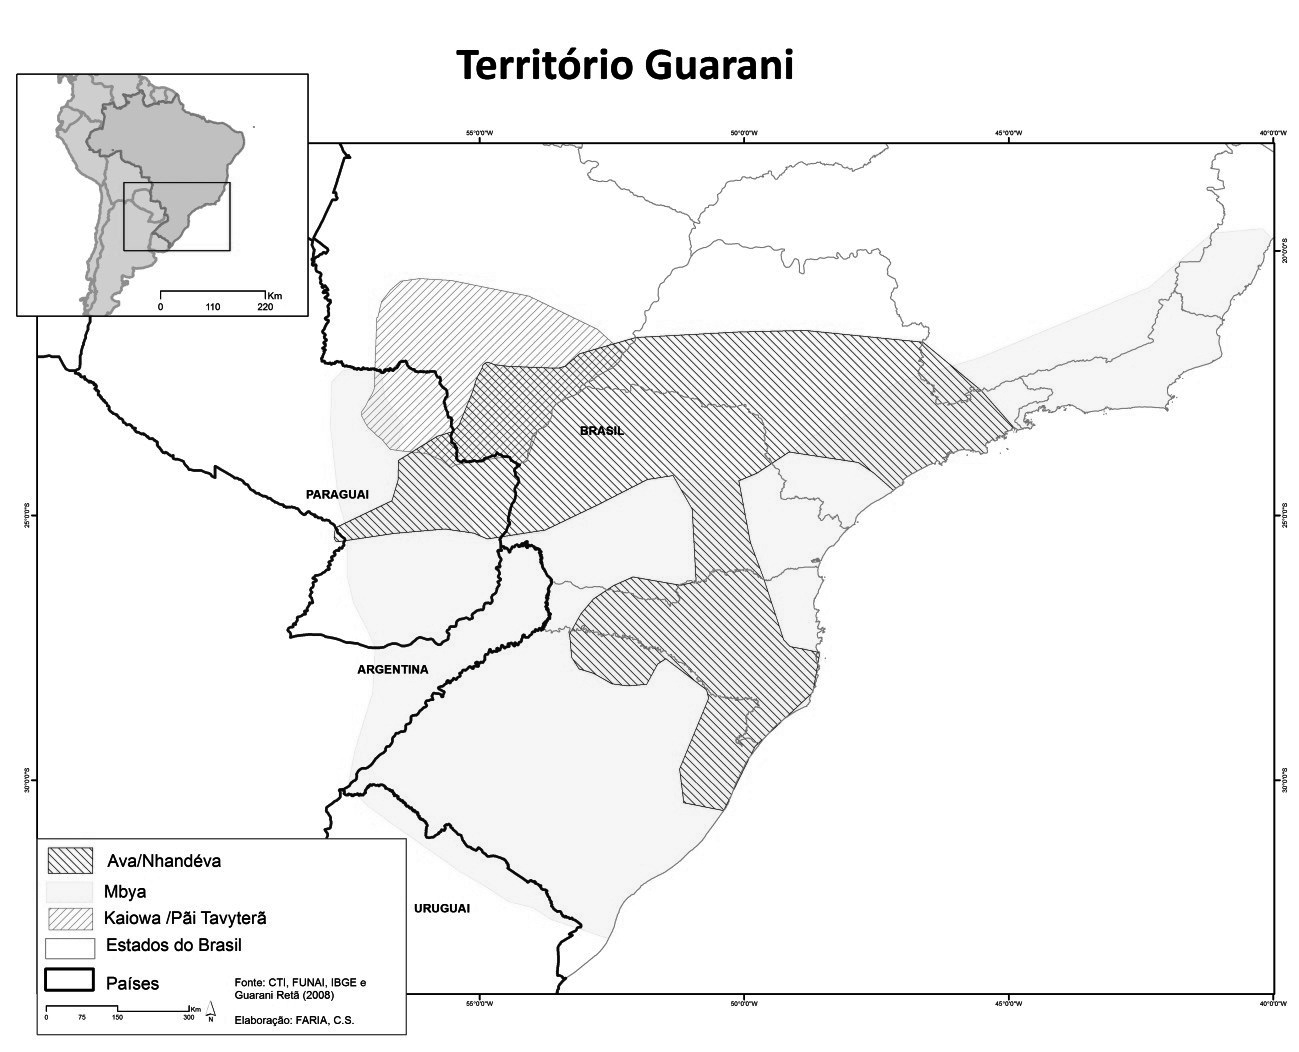
\includegraphics[width=\textwidth]{./img/GUARANIS-img7.jpg}	
  \hfill
  \caption{Distribuição territorial atual das parcialidades Guarani. Elaboração: Camila Salles de Faria.}
\end{figure}

   % Unhandled or unsupported graphics:
%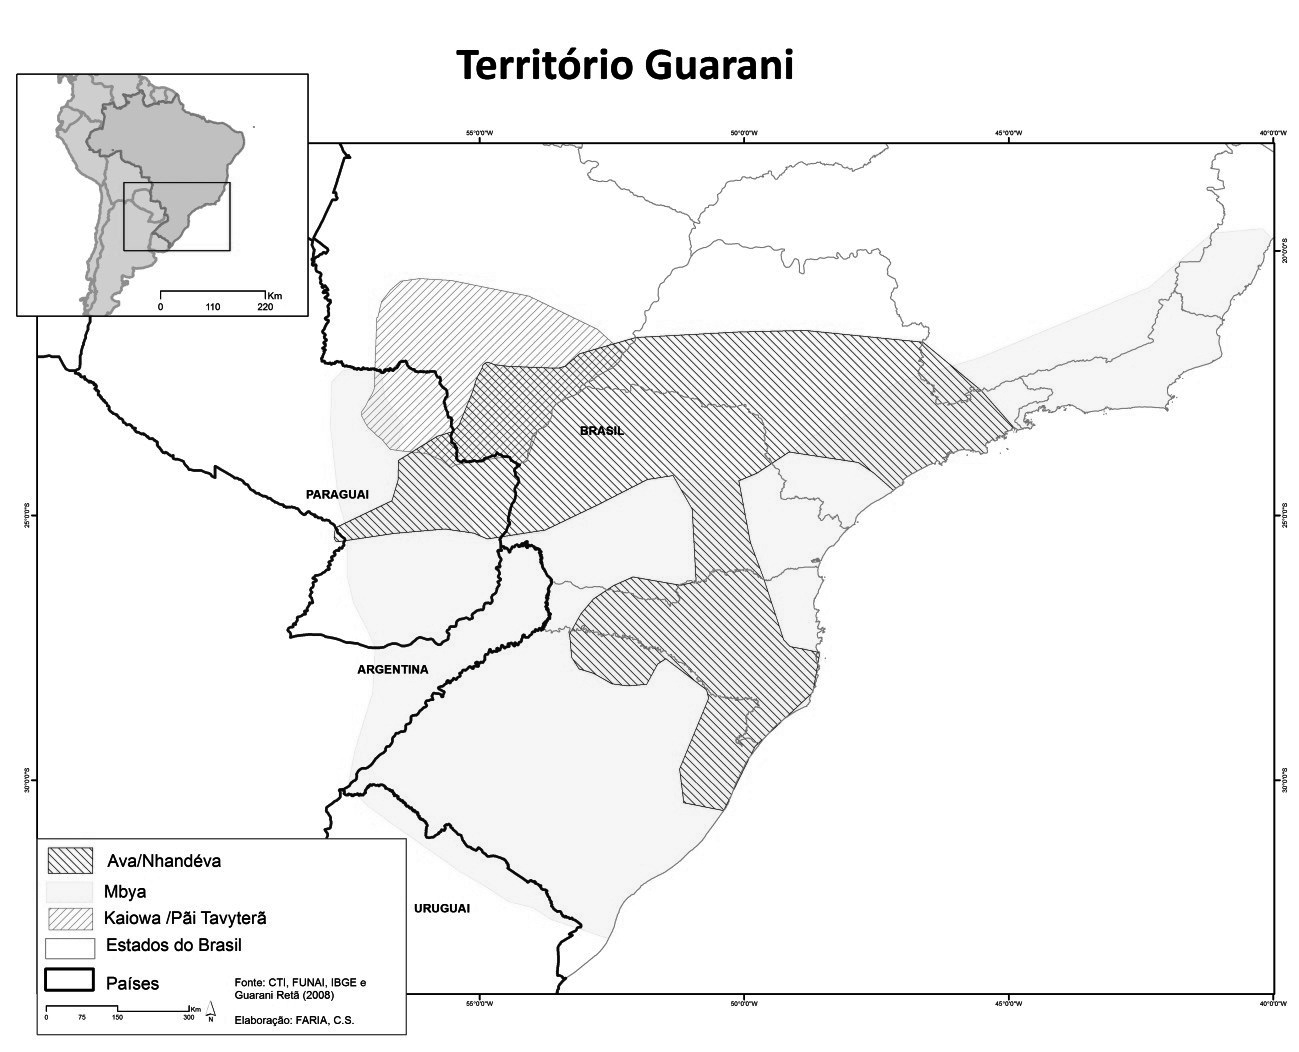
\includegraphics[width=\textwidth]{./img/GUARANIS-img7.jpg}
 

%Mapa 
%%\stepcounter{Mapa}{\theMapa} 
%– Distribuição territorial atual das
%parcialidades Guarani. Elaboração: Camila Salles de Faria.

Durante meu trabalho de campo na \versal{TI} Mbiguaçu/\versal{SC}, certo dia cheguei a
casa do casal de anciãos, onde encontrei Alcindo confeccionando um
pequeno balaio que lhe havia sido encomendado por uma vizinha. Na
ocasião, ele fez questão de destacar que aquilo não se tratava de um
\emph{ajaka}, como se chamam as cestarias mbya, mas que era um \emph{mbajo}, o cesto
antigo dos Chiripa, fabricado com cipó. Chamou"-me a atenção o destaque
dado a tal diferenciação na cestaria, por ela também ter sido
utilizada, nos anos 1930, pelo padre Franz Müller (1989) como exemplo
de diferenças linguísticas, ideológicas e simbólicas entre os três
agrupamentos Guarani presentes na região do Alto Paraná, que ficaram
conhecidos pelas designações Mbya, Nhandéva (ou Chiripa) e Kaiowa. A
presença dessa grande diversidade na população guarani já havia sido
apontada naquela região por Nimuendaju (1914) alguns anos antes.

Um investimento importante na caracterização das parcialidades Guarani
na etnografia são os diversos estudos feitos por Cadogan (1997;
1960; 1971), que trouxeram à luz diversas
especificidades dos grupos Mbya no Paraguai, além de apontamentos
comparativos com os Ava"-Chiripa (1959) no Alto Paraná. Menciono ainda
duas referências que considero pontos"-chave sobre
especificidades dos grupos Guarani no Paraguai, que nos anos 1970
ampliam os apontamentos feitos por Cadogan, quais sejam as etnografias
de Bartolomé (1977), sobre os Avá-Katu"-Ete, e de Melià,
George \& Friedl Grünberg (1976), sobre os Paí-Tavyterã. Em linhas
gerais, estes estudos vão caracterizar as parcialidades como sendo os
Paĩ/Kaiowá descendentes da redução
Itatim, com influência mais explícita do missionamento jesuítico; os
Ava"-Chiripa como grupos derivados da redução de Tarumã, com relações
mais intensas com os colonos; e os Mbya como um agrupamento mais
hermético, que pode manter"-se mais afastado dos não"-indígenas. 

A~obra de Egon Schaden (1962), em seus ``aspectos fundamentais
da cultura guarani'', delineia as especificidades das parcialidades no
Brasil, tornando"-se referência para as pesquisas posteriores que se
dedicaram a compreender a dinâmica territorial dos Guarani e das
relações entre as parcialidades. Apesar de sua inovadora modernidade,
parece"-me que a obra de Schaden peca por seu enfoque na ``aculturação'',
o que não ofusca a sua qualidade descritiva e analítica. Para compreender as articulações entre as
parcialidades nos estados do sul do Brasil, o estudo se faz incipiente,
estando restrito às aldeias Palmeirinha, no Paraná, e Limeira, no oeste
de Santa Catarina. Mas tem o mérito de identificar, já nos anos 1940, a
movimentação de grupos Mbya pelo Rio Grande do Sul, avançando pelo
litoral catarinense em direção à região sudeste do país. Os grupos
tomados como referência por Schaden para descrição dos Ava"-Chiripa, aos
quais ele chama de Nhandéva e ``Mbüa'', são aqueles que à época
habitavam o estado de São Paulo, deixando um lapso com relação à sua
presença na região sul.

A~presença dos coletivos Guarani no sul do Brasil passou a ser objeto de
estudos mais detalhados somente nos últimos quinze anos e, embora ainda
careça de uma síntese abrangente, estes trabalhos permitem uma análise
dessas intrigantes articulações e transformações entre os grupos no
nível regional. 

Inicio a reflexão a partir da dissertação de Garlet (1997), que
mapeia a mobilidade de grupos Guarani no Rio Grande do Sul, aos quais
ele chama Mbya, trazendo uma importante reflexão sobre a continuidade
entre estes e aqueles que se encontravam nas selvas do Alto Paraná
(Paraguai) e Misiones (Argentina) no fim da Guerra do Paraguai, em
1870. Podemos considerar que estudos como os de Ciccarone
(2001), Ladeira (2007; 2008), Rodrigues (1999),
Litaiff (1996 e 1999) e Vietta (1992), entre outros, são
pioneiros em descrever com maior detalhamento diversos aspectos
instigantes desta mobilidade mbya pelo interior do Rio Grande do Sul,
bem como seu avanço pelo litoral atlântico até a região sudeste do país
e sua articulação com outros grupos que já se encontravam naquela
região. Entretanto, faço a ressalva de que, com algumas exceções, tais
estudos pecam em não reconhecer apropriadamente a sobreposição e a
co"-habitação entre tais grupos mbya com os Chiripa, que possuíam
articulações relativamente estreitas, possivelmente anteriores a esta
movimentação territorial.

Os primeiros estudos de fôlego que tentam abarcar estas articulações e
transformações entre as parcialidades Mbya e Chiripa no sul do Brasil
são as etnografias escritas por Mello (2001; 2006;
2007), que nos trazem um preciso delineamento das relações entre esses
grupos no litoral catarinense e no interior do Rio Grande do Sul. A
autora demonstra como estes grupos se organizaram pela
sobreposição de sua mobilidade e co"-habitação, constituindo diversos
tipos de alianças no decurso do processo histórico. Entretanto, nesta
esteira podemos somar outros estudos que apontam para este convívio
entre as parcialidades, como a tese de Darella (2004), a
dissertação de Gobbi (2008) e outros, entre os quais incluo a
minha própria dissertação (Oliveira, 2011). 

Penso que tal lapso possa ter influenciado algumas outras etnografias
posteriores que acabam por reificar uma totalidade mbya homogênea, sem
dar conta de forma apropriada da diversidade desta composição. Podemos
dizer que, devido a complexidade do tema, este tem sido um assunto
evitado em diversas etnografias às quais tive acesso. Além disso,
podemos pensar que essa unificação em torno de uma identidade mbya é
uma questão incorporada pelos Guarani no sul do Brasil, o que
possivelmente contribui em dificultar a percepção de diferenças sutis
entre as parcialidades, imiscuídas em relações de aliança a parentesco.

\section{Chiripa, Paĩ, Tambeope}

Desde o início de meu trabalho de campo na \versal{TI} Mbiguaçu, \versal{SC}, para
realização de minha dissertação de mestrado (Oliveira, 2011),
chamava"-me atenção o fato de meu casal interlocutor, Alcindo Moreira e
Rosa Mariani Cavalheiro, que em linhas gerais se auto"-identifica aos
não"-índios como mbya, apontar recorrentemente a sua diferença a outros
grupos Guarani por serem do ``costume chiripa''. Tal assertiva passou a
fazer sentido a partir de sinais diacríticos que apontava o casal como
marcadores de sua diferenciação, que a todo momento faziam referência
aos aldeamentos em que o casal de anciãos havia vivido sua infância, no
Paraná. Optei por sistematizar quatro elementos os quais
inúmeras vezes ouvi serem referenciados pelo casal como marcadores de
diferenciação entre grupos Guarani Chiripa (que ficaram mais conhecidos
como Nhandéva), Paĩ (que ficaram mais conhecidos
como Kaiowa) e Tambeope (que vieram a ser conhecidos como Mbya), quais
sejam: a constância nos assentamentos, a indumentária, os hábitos
alimentares e a língua. 

A~constância nos assentamentos é um dos elementos apontados pelo casal
como diacrítico entre seus grupos Chiripa e Paĩ
em relação aos Tambeope. Segundo relatam, os primeiros reuniam grande
número de famílias em seus aldeamentos, estabelecendo"-se por longos
períodos de tempo em um mesmo lugar. Por vezes as aldeias Chiripa e
Paĩ abrigavam temporariamente famílias tambeope
errantes, que eram acolhidas como mão de obra em suas lavouras e na
criação de animais. Por diversas vezes ouvi alusões de que os demais
grupos ``educavam'' os Tambeope sobre os costumes da agricultura e a
religião dos Guarani. Obviamente a constância nos assentamentos está
imbricada a diversos outros aspectos do modo de vida, como as
atividades agrícolas e a sua mobilidade no território.

Outro elemento bastante evidente sobre a forma de se reconhecerem
mutuamente as parcialidades era a indumentária. As vestimentas eram
marcadores nítidos da diferença e da própria denominação das
parcialidades, sendo fabricadas com fios de algodão cru ou com fibras
de pyno (urtigão). Neste sentido, os Chiripa usavam calças compridas
chamadas de chiripas; os Pa${greek{~i}}$ utilizavam ponchos
longos que cobriam todo o corpo; e os Tambeope vestiam somente pequenas
batas atadas na cintura, chamadas de tambeo, motivo pelo qual foram por
vezes denominados na bibliografia como batícolas.

O~terceiro elemento apontado como fator de diferenciação era a alimentação, notavelmente associada a
construção do corpo para a atividade xamânica. Segundo os relatos de
Rosa e Alcindo, de forma geral os grupos Chiripa e
Paĩ praticavam restrições alimentares mais
rígidas. Os primeiros comiam somente rãs, peixes e eventualmente
lagartos, animais de sangue frio, centrando sua dieta no consumo de
bebida fermentada de milho, o \emph{kauĩ}; enquanto os
segundos criavam \emph{uru’ũ} (corvos), que eram a principal fonte proteica,
consumida junto aos produtos das roças e frutas coletadas nas matas. As
carnes de caça eram utilizadas sobretudo para o tratamento de doenças,
com o uso da gordura de animais silvestres na preparação de remédios.
Sobre os hábitos alimentares dos Tambeope, Alcindo e Rosa afirmam que
estes caçavam prioritariamente com o uso de armadilhas, sem seguirem
rígidas prescrições alimentares. Chamam a atenção para o fato de que os
grupos Tambeope estavam em intensa mobilidade, viajando longos meses em
jornadas em direção ao litoral atlântico. 

O~quarto elemento que aponto é a língua.
Podemos dizer que os dialetos nhandéva e kaiowa são mais próximos entre
si do que o mbya. O~casal marca que
tal fator aumentava a articulação entre os Chiripa e os
Paĩ, ao passo em que os distanciava dos Tambeope,
com quem tinham maior dificuldade para conversar. Alcindo e Rosa fazem
menção aos dialetos nhandéva e kaiowa como sendo a ``língua antiga'',
chamando à atenção o fato de atualmente terem adotado o dialeto mbya em
sua fala cotidiana. Esse é um aspecto importante para pensarmos as
transformações ocorridas no grupo Chiripa/Paĩ a
partir de suas articulações com os grupos Mbya ao longo de sua
mobilidade no território.

\section{A~configuração Mbya}

Em suas narrativas, Alcindo e Rosa costumam usar como marco de sua
história de vida o ``tempo em que não existia \emph{jurua}'', a mobilidade
decorrente da invasão de suas terras por colonizadores alemães e o
processo de demarcação do território no litoral de Santa Catarina.
Segundo o casal, sua idade é medida de fato pela ``taquara seca'',
que diz respeito ao período de florescimento do \emph{takua ete’i}
(taquara"-mansa), que acontece em média a cada 30 anos; como eles dizem
que teriam assistido tal fenômeno por três vezes, proponho
considerarmos que tais eventos tenham ocorrido a partir dos anos 1920.

A~sua história de vida tem início na região compreendida entre os rios
Iguaçu e Paraná, onde viviam em dois aldeamentos chamados Pari e
Piracanju, separados em um grupo familiar Paĩ e
outro Chiripa, que possuíam vários tipos de alianças entre si. O~casal
marca com precisão a articulação entre os grupos familiares dessas duas
aldeias, que permaneceram por diversos anos em assentamento constante,
em relação aos Tambeope, que eventualmente permaneciam por curtos
períodos abrigados em seus aldeamentos. Estas aldeias se desfazem a
partir do loteamento das terras no interior do Paraná, quando o grupo
familiar inicia um processo de mobilidade no território em busca de
espaços onde pudessem se reassentar e consolidar novos \emph{tekoha}. O~casal
Rosa e Alcindo passa a viver em peregrinação junto de seus pais,
oferecendo mão"-de"-obra em fazendas e circulando por diversas cidades
dos estados de Santa Catarina e Rio Grande do Sul. Neste movimento, o
casal participa da fundação de aldeamentos que atualmente ainda se
encontram consolidados nesses estados, como Mato Preto, Araçá’i, Campo
Molhado, Granja Vargas, Cacique Doble, Estiva, Cantagalo, Morro dos
Cavalos, Mbiguaçu, entre outros\footnote{Cf. Vietta (1992); Garlet
(1997); Gobbi (2008); Mello (2001; 2006; 2007); Darella (2004);
Tommasino (2001); Ladeira (2007; 2008).}.

Existem cerca de trinta áreas de coabitação entre grupos Mbya e Chiripa
no sul do Brasil, que somam aproximadamente 5.500 índios (\versal{BRASIL}/\versal{SESAI},
2013). As articulações entre esses grupos, ocorridas ao longo deste processo
de intensificação da coabitação, promoveram além de laços matrimoniais
e alianças políticas e econômicas, uma aproximação em outros campos,
como o religioso e principalmente o linguístico, com a total
incorporação do dialeto mbya. Esta aproximação entre as duas
parcialidades, que passaram a se identificar com a designação Mbya,
teve efeito tanto em relações internas, com o estabelecimento de laços
matrimoniais e alianças políticas e econômicas, como na relação externa
na negociação por reconhecimento pelo Estado brasileiro.

\section{Os Nhandéva contemporâneos}

O~centro territorial dos Nhandéva é a região do Alto Paraná, onde
estavam intensamente concentrados no final do século \versal{XIX}, servindo de
mão de obra na logística da erva"-mate no Brasil e no Paraguai. Com o
avanço dos colonos paulistas e sulistas sobre o Paraná e o Mato Grosso
do Sul, no começo do século \versal{XX}, os Nhandéva sofrem uma drástica perda
de território e acabam por ser subjugados ao serviço braçal nas
fazendas ou removidos para as Reservas Indígenas no Mato Grosso do Sul,
no interior de São Paulo e do Paraná, ou ainda levados para o Paraguai.
É~neste período histórico que acontecem os movimentos migratórios
registrados por Nimuendaju (1987), marcando a etnologia Guarani ao
discorrer sobre a busca da ``Terra Sem Males''. Os Nhandéva fizeram a
migração para o litoral por duas rotas distintas, uma pelo interior do
Rio Grande do Sul e outra pelo interior do Paraná até São Paulo, em
parte delas estabelecendo coabitação com grupos Mbya, que vinham da
região de Misiones, Argentina, e do sul do Paraguai.

Como mencionado, os Nhandéva que na transição para o século \versal{XX}
migraram para o Rio Grande do Sul e Santa Catarina, bem como para o
interior de São Paulo, eram chamados pelos outros grupos de Chiripa.
Podemos delinear duas levas migratórias distintas de grupos Nhandéva
para o litoral e o interior de São Paulo, uma no começo do século \versal{XX},
relatada por Nimuendaju (1987), e outra a partir nos anos 1960, com a
expropriação do território no oeste do Paraná, no Paraguai e no Mato
Grosso do Sul. Atualmente existem doze áreas de coabitação entre
famílias Nhandéva e Mbya que somam um contingente de cerca de 3.500
pessoas.

Embora estas movimentações sejam ininterruptas, com idas e
vindas constantes de grupos familiares, elas se situam em momentos
coloniais específicos, uma no início da titulação das terras e a
exploração da mão"-de"-obra na madeira e na erva"-mate; outra no avanço da
ocupação efetiva do território por colonos (Myskyw, 2002; Cardoso \&
Westphalen, 1986; Ribeiro, 2002; Conradi, 2007). Nos anos 1970, com o
avanço da agricultura mecanizada e a construção da usina de Itaipu,
diversos grupos Nhandéva do Alto Paraná rumaram ao estado de São Paulo
por fugas e migrações voluntárias, articulando"-se com grupos Mbya que
faziam o mesmo percurso. A~dissertação de Pierri (2013) descreve
alguns desses grupos na região do Vale do Ribeira, falantes do dialeto
mbya.

Os grupos assentados em reservas mais antigas, como as \versal{RI}s Araribá e
Serra do Itatins, mantiveram"-se resistentes à presença de grupos Mbya,
não incorporando costumes religiosos e tampouco o dialeto,
autoidentificando"-se normalmente como Nhandéva. Alguns desses grupos
constituíram novos etnônimos de diferenciação, recusando também o termo
\emph{chiripa}, considerado pejorativo, e passando a se autoidentificarem com
Tupi"-Guarani. Desta forma, percebe"-se que de fato existe um contraste
entre os Tupi"-Guarani e Nhandéva de São Paulo com os Chiripa do sul do
Brasil.

Os Nhandéva no Mato Grosso do Sul estavam concentrados sobretudo na
bacia mais ao sul do estado, na divisa com o Paraguai, sendo recolhidos
compulsoriamente para as reservas para a instalação das grandes
fazendas na região. Nas Reservas Indígenas foram colocados em convívio
forçado com grupos Kaiowa, estabelecendo relações de conflito e
aliança. Este período de desterritorialização dos Guarani no Mato
Grosso do Sul é chamado por eles de \emph{sarambi} --- espalhamento ---, ao qual
se referem em português como ``o tempo do corre"-corre'', um deslocamento
desordenado em função da violência da colonização. Ocupam atualmente
nove Terras Indígenas, em sua maioria compartilhadas com outros grupos,
além de mais de 20 acampamentos que aguardam providências para
regularização fundiária, somando um contingente de mais de 20 mil
índios (\versal{SESAI}, 2013). De forma geral, autoidentificam"-se simplesmente
como Guarani, como um diferenciador em relação aos Kaiowa, com quem
mantém um estreito vínculo político em função da luta pela demarcação
de terras (Pereira, 1999; Pimentel, 2012), sendo praticamente nula
qualquer presença Mbya entre esses grupos.

Há ainda outro contraste importante nas transformações nos Nhandéva
contemporâneos, que são aqueles que não empreenderam grandes movimentos
migratórios em direção ao atlântico, mas permaneceram nas margens
brasileira e paraguaia do Rio Paraná e na bacia do Iguatemi e na Serra
do Maracaju, no Mato Grosso do Sul. Os Nhandéva paranaenses se
autoidentificam como Ava"-Guarani, mesmo nomenclatura utilizada no
Paraguai e historicamente atribuída ao grupo, sendo muito próximos os
Guarani sul"-mato"-grossenses. O~grupo teve maior visibilidade nos anos
1970 e 1980 em função da construção da usina de Itaipu que, associada
ao processo de esbulho praticado pelos colonos, pode ter removido cerca
de seis mil índios, que ocupavam mais de 40 aldeias (Carvalho, 2013;
Peralta, 1995; Guaska, 2012), no oeste do Paraná. Estes índios da
Tríplice Fronteira trabalharam nos ciclos econômicos da região e
permaneceram sujeitos a diversos tipos de violência para expropriação
de suas terras. Atualmente, estão organizados em cerca de 20 aldeias,
que somam aproximadamente três mil índios (\versal{SESAI}, 2013), sendo que
somente três delas estão regularizadas.

A~Tríplice Fronteira é uma zona de micromobilidade Guarani que por sua
posição geográfica proporciona a influência dos grupos Mbya de
Missiones, na Argentina, e de grupos Ava dos departamentos de Alto
Paraná e Canindeyu, no Paraguai; como bem demonstra a tese de Evaldo
Mendes da Silva (2007). É~importante pontuar ainda que a presença de
pessoas Mbya e Kaiowa entre os Ava"-Guarani é comum, porém bastante
discreta, uma vez que muitos Ava foram removidos para as reservas
Kaingang no interior do Paraná, como Mangueirinha, Rio das Cobras e
Marrecas, coabitando com grupos \emph{mbya}, sendo que outros foram deslocados
para as reservas Kaiowa, como Dourados, Amambai e Caarapó. Seus
vínculos se estendem ainda às reservas Nhandéva no Mato Grosso do Sul,
como Porto Lindo, Pirajui, Sombrerito, Jaguapiré, o que lhes permitiu
articulação com o movimento indígena Aty Guasu. Além disso, diversas
famílias Ava"-Guarani migraram ainda nos anos 1960 e 1970 para áreas
mais distantes, como São Paulo, Rio de Janeiro e o litoral do Paraná,
em função da construção da usina de Itaipu. Desta forma, seus vínculos
de aliança alcançam ainda algumas aldeias próximas ao litoral, com
grupos que tem identificação com a etnogênese do Povo Mbya,
aproximando"-se de sua principal organização etnopolítica, a Comissão
Guarani Yvyrupa.

   % Unhandled or unsupported graphics:
%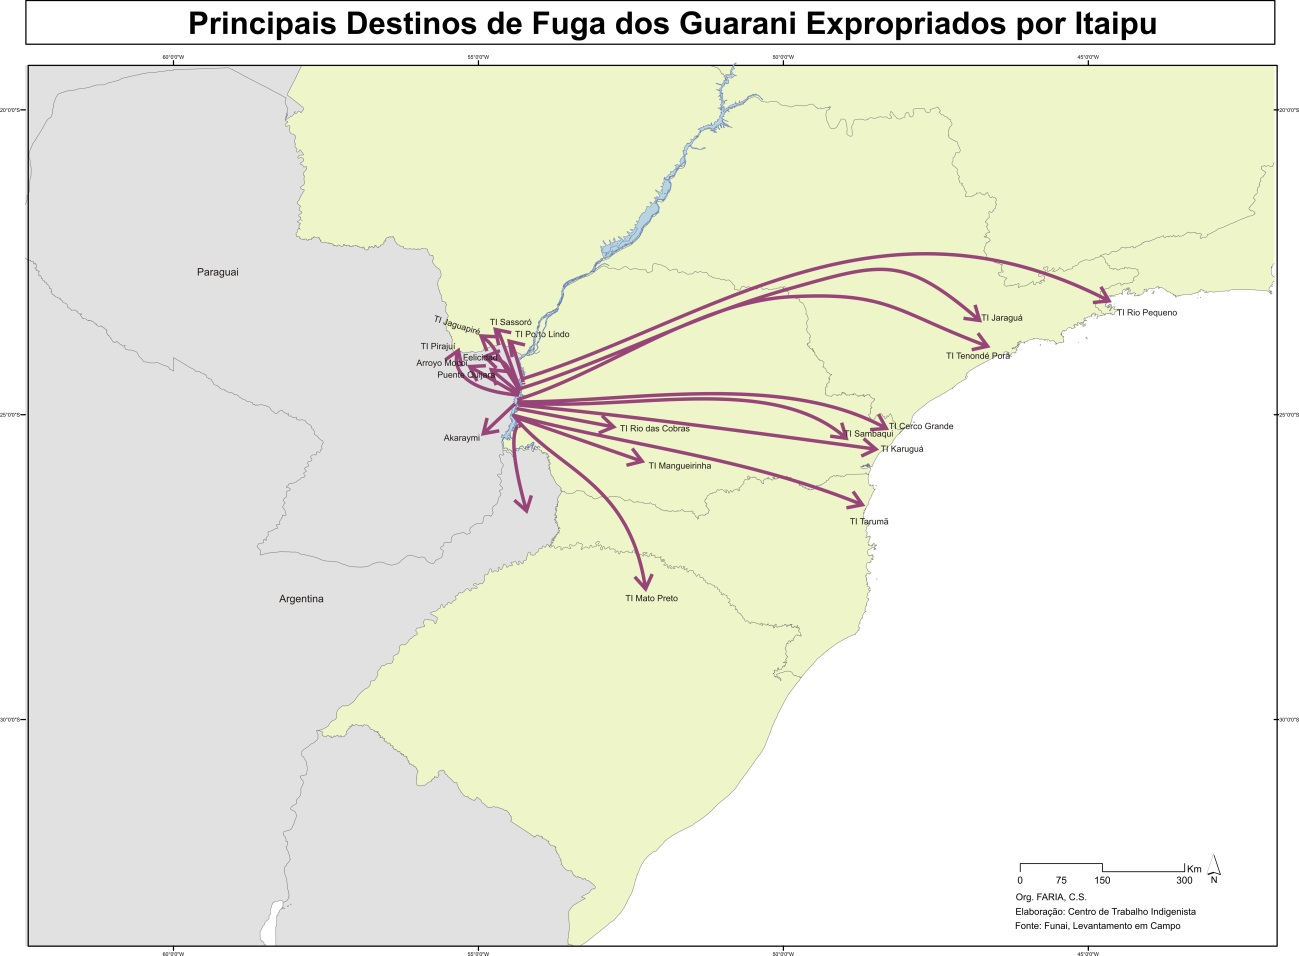
\includegraphics[width=\textwidth]{./img/GUARANIS-img8.jpg}
 \begin{figure}
  \centering
 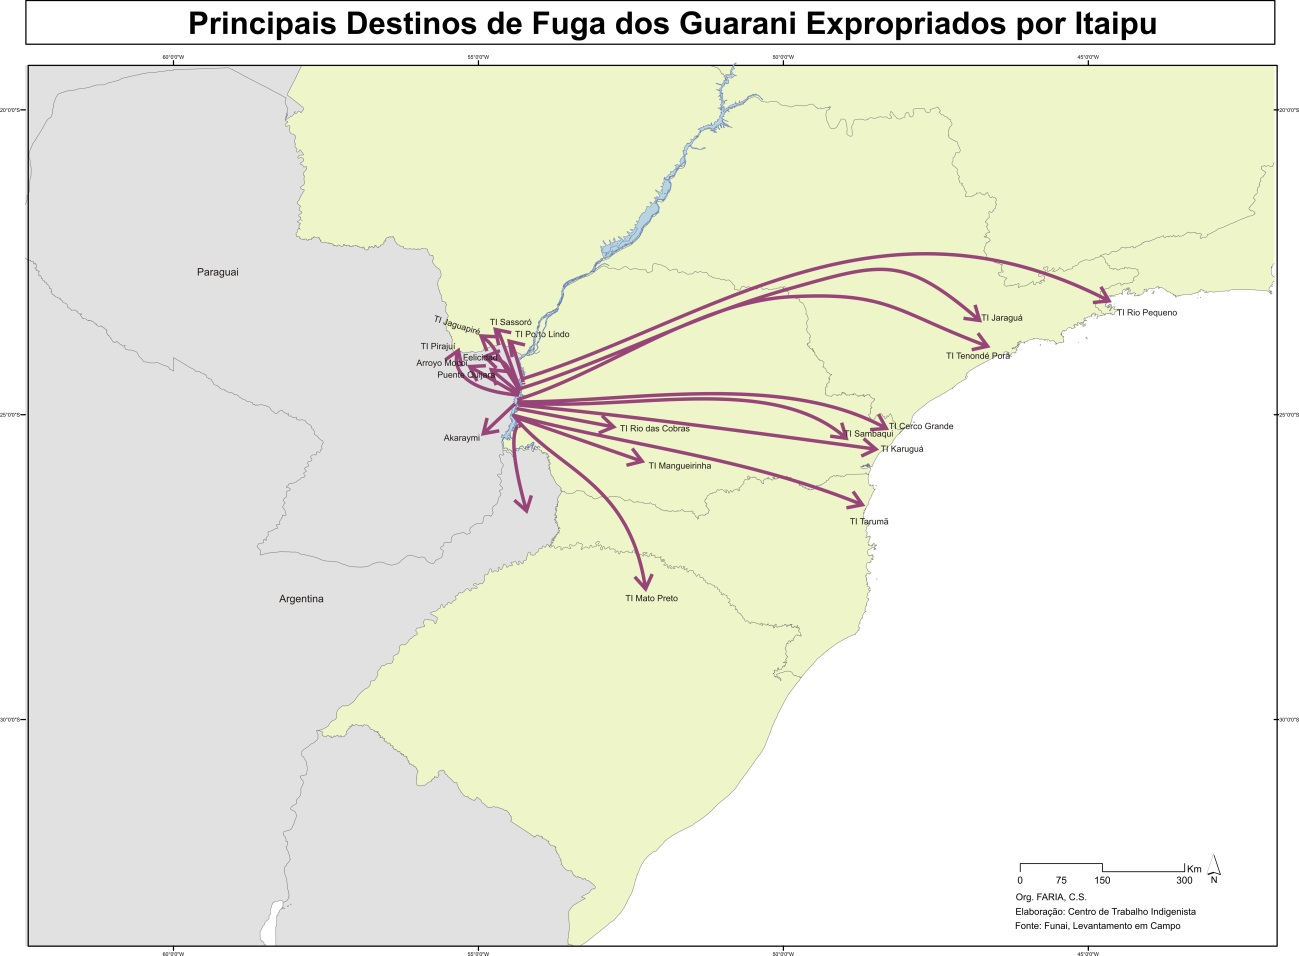
\includegraphics[width=\textwidth]{./img/GUARANIS-img8.jpg}	
  \hfill
  \caption{Rotas de migração dos Nhandéva a
partir dos anos 1970. Elaboração: Camila Salles de Faria.}
\end{figure}

%Mapa 
%\stepcounter{Mapa}{\theMapa} 


Percebemos que a parcialidade tradicionalmente classificada como
Nhandéva compõe atualmente uma gama de grupos indígenas brasileiros e
transfronteiriços, cujas especificidades estão associadas com as suas
particularidades históricas. A~etnologia guarani ainda carece de uma
obra de síntese abrangente sobre a diversidade dos Nhandéva
contemporâneos no Brasil. Esta seria uma
contribuição substancial para o conhecimento sobre o povo guarani em
sua pluralidade atual. 

\section{Referências}

\begin{Parskip}
\versal{BARABAS}, Alicia M. ``Los derechos indígenas, la antropología jurídica y
los movimientos etnopolíticos''. \emph{Ilha}, vol.~10, n.~1, 2008.

\versal{BARBOSA}, Pablo Antunha \& \versal{MURA}, Fabio. ``Construindo e reconstruindo
territórios Guarani: dinâmica territorial na fronteira entre Brasil e
Paraguai (sec. \versal{XIX}-\versal{XX})''. \emph{Journal de la société des américanistes}, vol.~97, n.~2,
2011. 

\versal{BARTOLOMÉ}, Miguel. \emph{Orekuera Royhendu (Lo que escuchamos en
sueños): Shamanismo y religión entre los Ava"-Katu"-Ete del Paraguay}.
México: Instituto Indigenista Interamericano, 1977.

\_\_\_\_. \emph{Procesos interculturales: antropología política
del pluralismo cultural en América Latina}. México: Siglo \versal{XXI} Editores,
2006.

\_\_\_\_. ``Oguerojera (desplegarse) - la etnogenesis del
pueblo mbya"-guarani''. \emph{Ilha}, 10(1), 2008.

\versal{BASINI} \versal{RODRIGUES}, José E. \emph{Estratégias econômicas, políticas e religiosas
na mito"-práxis mbyá-guarani}. Dissertação de Mestrado. \versal{UFRGS}, 1999.

\versal{BRASIL}. \versal{SESAI} (Secretaria especial de Saúde Indígena). \emph{\versal{SIASI} — Sistema
de Informação de Atenção à Saúde Indígena}. Brasília: Ministério da
Saúde/\versal{SESAI}, 2013.

\versal{BRIGHENTI}, Clóvis.\emph{~Estrangeiros na própria terra:~presença
Guarani e Estados Nacionais}.~Chapecó: \versal{ARGOS}/Ed. da \versal{UFSC}, 2010. 

\versal{CADOGAN}, León. \emph{Ayvu rapyta: textos míticos de los Mbyá-Guaraní del
Guairá}. Asunción: Ceaduc"-Cepag, 1997 [1959].

\_\_\_\_. ``Como interpretan los Chiripá (Avá Guaraní) la
danza ritual''. \emph{Revista de Antropologia}, vol.~7, n.~1-2, 1959.

\_\_\_\_. ``En torno de la aculturación de los Mbya"-Guaraní
del Guairá''. \emph{América Indígena}, vol.~20, n.~2, 1960. 

\_\_\_\_. \emph{Ywyra Ñe’ery: fluye del árbol la palabra.
Sugestiones para el estudio de la cultura guaraní}. Asunción: \versal{CEPAG},
1971.

\versal{CARDOSO}, Jayme; \versal{WESTPHALEN}, Cecília. \emph{Atlas Histórico do Paraná}.
Curitiba: Livraria do Chaim, 1986.

\versal{CICCARONE}, Celeste. \emph{Drama e sensibilidade: migração, xamanismo e
mulheres mbya guarani}. Tese de Doutorado. \versal{PUC}-\versal{SP}, 2001.

\versal{CONRADI}, Carla. \emph{As ações do Estado Nacional e a
trajetória política dos Guarani Ñandeva no Oeste do Paraná (1977-1997)}.
Dissertação de Mestrado. \versal{UFGD}, 2007.

\versal{DARELLA}, Maria Dorothea. \emph{Ore Roipota Yvy Porã, Nós queremos terra boa:
territorialização guarani no litoral de Santa Catarina, Brasil}. Tese de
Doutorado. \versal{PUC}-\versal{SP}, 2004.

\versal{GARLET}, Ivori. \emph{Mobilidade mbyá: história e significação}.
Dissertação de Mestrado. \versal{PUC}-\versal{RS}, 1997.

\versal{GOBBI}, Flávio S. \emph{Entre parentes, lugares e outros: traços na
sociocosmologia guarani no sul}. Dissertação de Mestrado. \versal{UFRGS}, 2008.

\versal{GUASKA}, Enrique. ``Del canto al llanto. Situación de las comunidades
indígenas afectadas por la represa de Itaipú''. \emph{Acción}, vol.~157, 2012.

\versal{LADEIRA}, Maria Inês. \emph{O~caminhar sob a luz. Território mbya à
beira do oceano}. São Paulo: \versal{UNESP}, 2007.

\_\_\_\_. \emph{Espaço geográfico guarani"-mbya: Significado,
constituição e uso}. São Paulo: Edusp, 2008.

\versal{LITAIFF}, Aldo. \emph{As divinas palavras: identidade étnica dos Guarani"-Mbyá}.
Florianópolis: \versal{UFSC}, 1996.

\_\_\_\_. \emph{Les fils du soleil: mythes et pratiques dês
indiens mbya"-guarani du littoral du Brésil}. Tese de Doutorado.
Université de Montréal, 1999.

\versal{MELIÀ}, Bartolomeu; \versal{GRÜNBERG}, Friedl; \versal{GRÜNBERG} Georg. \emph{Los Pai"-Tavyterã.
Etnografía guaraní del Paraguay contemporáneo}. Asunción: Centro de
Estudios Antropológicos de la Universidad Católica, 1976.

\versal{MELIÀ}, Bartomoleu. \emph{El Guarani conquistado y reducido: ensayos de
etnohistoria}. Asunción: Biblioteca Paraguaya de Antropología, 1986.

\_\_\_\_. ``A~terra sem mal dos Guarani: economia e profecia''. \emph{Revista de
Antropologia}, vol.~33, 1990. 

\_\_\_\_. \emph{El Guarani: experiencia religiosa}. Asunción: Ceaduc"-Cepag, 1991.

\versal{MELLO}, Flávia. \emph{Aata tapé rupy, seguindo pela estrada:~uma
investigação dos deslocamentos territoriais de famílias mbyá-guarani no
sul do Brasil}.~Dissertação de Mestrado. \versal{UFSC}, 2001.

\_\_\_\_. \emph{Aetchá Nhanderukuery Karai Retarã. Entre Deuses e Animais:
Xamanismo, Parentesco e transformação entre os Chiripá e Mbyá}. Tese de
Doutorado. \versal{UFSC}, 2006. 

\_\_\_\_. ``Mbyá e Chiripá: identidades étnicas, etnônimos e autodenominações
entre os Guarani do sul do Brasil''. \emph{Tellus}, vol.~7, n.~12, 2007.

\versal{MÜLLER}, Pe. Franz. \emph{Etnografia de los Guarani del Alto Parana}. Buenos
Aires: \versal{CAEA}, 1989.

\versal{MYSKIW}, Antonio. \emph{Colonos, posseiros e grileiros: conflitos de
terras no Oeste Paranaense (1961/66)}. Dissertação de Mestrado.
\versal{UFF}-\versal{UNIOESTE}, 2002.

\versal{NIMUENDAJU}, Curt. \emph{As lendas de criação e destruição do mundo como
fundamentos da religião dos Apapocúva"-Guarani}. São Paulo: Hucitec/\versal{USP},
1987 [19l4].

\versal{OLIVEIRA}, Diogo. \emph{Arandu Nhembo’ea: Cosmologia, Agricultura e Xamanismo
entre os Guarani"-Chiripá no litoral de Santa Catarina}. Dissertação de
Mestrado. \versal{UFSC}, 2011.

\versal{PERALTA}, Raquel. \emph{Los impactos de la Itaipú y las respuestas a los
mismos, de los Avá Chiripá, de acuerdo a su filosofía sobre la tierra}.
Monografía, 1995.

\versal{PEREIRA}, Levi Marques. \emph{Parentesco e organização social kaiowá.
Dissertação de Mestrado}. \versal{UNICAMP}, 1999.

\versal{PIMENTEL}, Spensy K. \emph{Elementos para uma teoria política kaiowá e guarani}.
 Tese de Doutorado. \versal{PPGAS}-\versal{USP}, 2012.

\versal{RIBEIRO}, Sara. \emph{O~horizonte é a terra: manipulação da
identidade e construção do ser entre os guarani no Oeste do Paraná
(1977-1997)}. Tese de Doutorado. \versal{PUC}-\versal{RS}, 2002.

\versal{SCHADEN}, Egon. \emph{Aspectos fundamentais da cultura guarani}. São Paulo:
Difusão Europeia do Livro, 1962.

\versal{SILVA}, Evaldo Mendes da. \emph{Folhas ao vento: a micromobilidade de grupos
Mbya e Nhandéva (Guarani) na Tríplice Fronteira}. Tese de Doutorado. \versal{PPGAS}-Museu Nacional, 2007.

\versal{VIETTA}, Katya. \emph{Mbya: guarani de verdade}. Dissertação de Mestrado. \versal{UFRGS}, 1992.
\end{Parskip}

\clearpage

\vspace*{\fill}

\begin{flushright}
\begin{minipage}[c]{0.85\textwidth}
\raggedleft
\footnotesize
\emph{Os pesquisadores que trabalham com os Guarani têm enfrentado questões em
que a bibliografia clássica deixou uma lacuna, como do que se fala
quando se menciona ``coletivos'', e do que se fala quando se menciona
``redes''. O~culturalismo que guiou o trabalho de missionários e etnólogos
na virada do século \versal{XIX} para o \versal{XX} buscava recuperar a diversidade na
cultura material e em outros aspectos para a construção das etnias,
como se fossem totalidades fechadas. Mas se pode reconhecer na
documentação histórica desde o século \versal{XVII} a organização em redes. O
critério de totalidades étnicas como construção da diferença aparece
como resultante do contato com os agentes coloniais.}

\smallskip
\hspace*{\fill}--- Marta Amoroso
\end{minipage}
\end{flushright}

\thispagestyle{empty}

\chapter*{Um nome que faz diferença\\
%\bigskip
\large{\emph{Reflexões com famílias tupi guarani}}}

\addcontentsline{toc}{chapter}{Um nome que faz diferença,
\scriptsize{\emph{por Lígia Almeida, Amanda Danaga e Camila Mainardi}}}

\begin{flushright}
\emph{Lígia R. Almeida\footnote{Doutora em antropologia social pelo
\versal{PPGAS}-\versal{USP}}, Amanda C. Danaga\footnote{Doutora em antropologia
social pelo \versal{PPGAS}-\versal{UFSC}ar.} e Camila Mainardi\footnote{Doutora em antropologia social pelo \versal{PPGAS}-\versal{USP}}}
\end{flushright}
\medskip
%\emph{Lígia R. Almeida}\footnote{* Doutora em antropologia social pelo
%PPGAS-USP.}, Amanda C. Danaga\footnote{** Doutora em antropologia
%social pelo PPGAS-UFSCar.}, Camila Mainardi\footnote{*** Doutora em
%=======
%\chapter{Um nome que faz diferença: reflexões com famílias tupi guarani.}
%
%\emph{Lígia R. Almeida}\footnote{* Doutora em antropologia social pelo
%PPGAS-USP.}, \emph{Amanda C. Danaga}\footnote{** Doutora em antropologia
%social pelo PPGAS-UFSCar.}, \emph{Camila Mainardi}\footnote{*** Doutora em
%>>>>>>> 738abc03eb2c0acf775166804e85af8f0ea8b0a3
%antropologia social pelo PPGAS-USP.}

\noindent
Existem famílias tupi guarani em diferentes locais no estado de São
Paulo: no litoral e sudoeste do estado, em áreas demarcadas ou não e,
ainda, em bairros de cidades como Mongaguá e Itanhaém.\footnote{Segundo
o site da Comissão Pró-índio de São Paulo, as \versal{TI} habitadas pelos Tupi
Guarani e seus municípios são: Araribá (Avaí); Bananal (Peruíbe);
Guarani do Aguapeú (Mongaguá); Serra de Itatins (Itariri); Jaraguá (São
Paulo); Ribeirão Silveira (São Sebastião); Itaoca (Mongaguá);
Piaçaguera (Peruíbe); Renascer (Ubatuba); Barão de Antonina (Barão de
Antonina); Guarani de Itaporanga (Itaporanga) Tekoa Jaikoaty
(Miracatu); Paranapuã (São Vicente); Aldeinha (Itanhaem); Paraíso
(Iguape). Em algumas dessas aldeias há co"-residência entre os Tupi
Guarani, Guarani Mbya e Terena. Fonte: \emph{http://www.cpisp.org.br/indios/html/uf.aspx?ID=SP}, informações de
2012).} Neste texto privilegiamos as experiências de campo em três
contextos etnográficos: aldeia Yvy Pyhaú, aldeia Ywyty Guaçu (ou aldeia
Renascer) e nas aldeias da \versal{TI} Piaçaguera, localizadas respectivamente
nos municípios de Barão Antonina (sudoeste do estado de São Paulo),
Ubatuba (litoral norte do estado de São Paulo) e Peruíbe (litoral sul
do mesmo estado). Veremos que a noção de ``mistura''\footnote{Falas e
conceitos de nossos interlocutores tupi guarani serão grafados em
itálico no corpo do texto.}, evidenciada pelos usos e exegeses sobre a
autodenominação Tupi Guarani, perpassa os três contextos,
relacionando"-se com iniciativas de valorização cultural e de retomada
de terras tradicionais. A~autodesignação Tupi Guarani expressa a
``mistura'' que, segundo nossos interlocutores, é resultante de uma história
comum de intercasamentos entre diferentes povos, indígenas e não
indígenas. 

O~uso de termos e categorias classificatórias se apresenta como algo
problemático, na medida em que pode reificar fronteiras étnicas e
essencializar a configuração de grupos, ao ocultar as dinâmicas
relacionais entre eles e sua constante atualização. As denominações
étnicas fazem parte dessas dinâmicas relacionais que inventariam as
alianças que os grupos mantêm com os outros, sejam eles índios ou não
índios, de maneiras muito diversas. Sendo as relações entre estes
atores contextuais e baseadas em diferentes experiências, há a
necessidade de apreender os contextos de enunciação das denominações
étnicas. As famílias com quem fizemos pesquisa compartilham a
autodenominação Tupi Guarani, embora possam ser identificados por
outras, como por exemplo, a designação Guarani Nhandeva.

Em razão de especificidades históricas, linguísticas e culturais, uma
divisão em subgrupos foi estabelecida por Egon Schaden (1954)
constituindo os Nhandeva, Mbya e Kaiowá.

Pesquisas de Ladeira e Azanha (1987) já mencionavam o uso da
autodenominação Tupi Guarani por algumas famílias do litoral paulista,
as quais também são chamadas pelos Guarani Mbya de Xiripá. Tal
designação é vista como pejorativa pelos Tupi Guarani. Schaden (1954),
a despeito de ter nomeado um subgrupo como Nhandeva, reconhece ``essa''
expressão como a autodenominação de todos os Guarani, significando ``os
que são dos nossos''.

A~respeito da definição desse termo, Nimuendaju (1987: 7) comentou: ``Os
Guarani, ao falarem de si na sua língua, para designar nação ou horda,
empregam o termo Ñandeva, quando a pessoa com quem se fala pertence ao
grupo, e Oréva, quando pertence a uma outra tribo''.

Nos três contextos etnográficos abordados aqui, percebemos o uso do
termo \emph{nhandeva} para se referirem aos parentes e a outros índios. Fazem
uso de nhandeva não como um etnônimo, uma categoria fixa que remeteria
a uma etnia, mas como forma de identificar"-se enquanto índios. Empregam
o termo, em especial, em oposição aos não índios.\footnote{No caso da
Ywyty Guaçu, o termo é bastante acionado para identificar uma oposição
em relação às famílias guarani mbya, com quem mantêm co"-residência.} O
que implica considerar \emph{Nhandeva} como uma noção relacional, sujeita aos
contextos e aos atores em jogo.

As denominações étnicas são, em geral, construídas na interface com os
não índios, na relação com o Estado --- mas não só --- e são imputadas de
maneira arbitrária, como no caso da etnônimo Nhandeva. Para o caso das
famílias tupi guarani, apontamos que estas não aceitaram um nome
imposto pelos não índios, mas trataram de lhes ensinar que são Tupi
Guarani. A~autodesignação expressa a ``mistura'', os casamentos entre Tupi
e Guarani, e também com outros índios e não índios como constituintes
da pessoa Tupi Guarani, sendo aquilo que a singulariza e não o que a
descaracteriza, como pensam alguns.

Apesar de compartilharem o uso da autodenominação Tupi Guarani, os
contextos que abordamos aqui possuem especificidades e autonomia. Neste
texto temos como objetivo mostrar que ser Tupi Guarani inclui uma
diversidade de possibilidades e que, no limite, uma aldeia pode trazer
à tona questões sobre as outras. Assim, apostamos que o conjunto
diverso de experiências vivenciadas em campo\footnote{Importante
pontuar que as autoras do texto não realizaram suas pesquisas de campo
conjuntamente. Lígia R. de Almeida pesquisa as famílias tupi
guarani da aldeia Ywy Pyhaú, Amanda C. Danaga na aldeia Renascer e
Camila Mainardi, nas Terra Indígena Piaçaguera.} exprime aspectos do
que é ser Tupi Guarani --- condição jamais dada, e sim constituída por
relações em constante reconfiguração. Seguimos, então, com os contextos
mencionados para tratar de questões que interessam aos nossos
interlocutores de modos e intensidades diferentes: a ``mistura'' e os
casamentos, as iniciativas de valorização cultural\footnote{Cultura
aqui em seu sentido aspeado, como sugere Manuela Carneiro da Cunha para
enfatizar o uso local que se faz da categoria cultura, lembrando que ``a
cultura de que falam os antropólogos não é a mesma da que falam os
povos indígenas'' e que cultura e ``cultura'' não pertencem ao mesmo
universo do discurso (2009: 313).}, as disputas territoriais e os
processos de demarcação da terra. 

\section{Aldeia Ywy Pyhaú: da luta pela terra ao fortalecimento da cultura}

A~aldeia Ywy Pyhaú está localizada no município de Barão de Antonina,
sudoeste do estado de São Paulo. Até o ano de 2014 era formada por
cinco famílias, somando um total de 30 pessoas.\footnote{Vale lembrar
que esses números são variáveis, pois dependem da chegada e partida de
pessoas e famílias.} A~terra onde está localizada passa atualmente por
um processo de regularização fundiária que se iniciou no ano de 2007, a
partir de uma palestra ministrada na Universidade Estadual Paulista
(\versal{UNESP}) de Araraquara pelo então cacique Marcílio
Marcolino. \footnote{Esta Mesa Redonda foi idealizada pelo Centro de
Estudos Miguel Ángel Menéndez (\versal{CEIMAM}) no evento ``Ameríndia'', que ocorreu
em 2007.} Junto a antropólogos e membros do Ministério Público, o
cacique discursou sobre a importância da terra para sua família Tupi
Guarani, fazendo críticas ferrenhas ao tratamento conferido aos povos
indígenas no estado de São Paulo, baseado em paradigmas aculturativos e
de perda cultural. Em suas palavras, ``nos tratam como povos extintos''. O
mesmo problema foi apontado em outro contexto por D. Juraci, a pessoa
mais velha da aldeia Ywy Pyhaú:

\begin{quote}
\noindent
Mas como nós desaparecemos se nós estamos aqui, nossa língua está aqui,
nossa cultura está aqui? Nós falamos no verdadeiro Tupi antigo, nós
sempre fomos Tupi Guarani, o branco que quis mudar isso. (Aldeia Ywy
Pyhaú, junho, 2010).
\end{quote}

Dessa palestra surgiu uma carta reivindicando a constituição de um grupo
técnico para realização dos estudos da terra. Na mesma ocasião,
Marcílio fez questão de enfatizar que além de terra era preciso
garantir o direito de sua família ``viver na cultura'', de ``ser Tupi
Guarani''. E~foi assim, junto às reivindicações pela terra e à busca de
garantia de que poderiam, tal qual ``os antigos''\footnote{``Viver como os
antigos'', segundo moradores de Ywy Pyhaú, pressupõe uma ``terra boa'', isto
é, com mata, caça e rios. Também uma alimentação composta menos de
produtos industrializados e mais de seus próprios cultivos, contando
com milho e mandioca para acompanhar a carne assada. Pressupõe ainda
que tenham força (\emph{mbareté}) e concentração suficientes para dançar e
cantar, tornando"-se leves para ``subir para \emph{Nhanderu}'' e ouvir o que ele
tem a lhes contar. O~cuidado entre parentes é enfatizado como
fundamental para a aquisição de tais qualidades.}, viver em uma ``terra
boa'' e próximos a \emph{Nhanderu}, que iniciaram, em 2010, um movimento pelo
reconhecimento enquanto um grupo indígena diferenciado. Diferença esta
marcada pela autodenominação Tupi Guarani, visto que eram conhecidos
até então como Guarani Nhandeva. Segundo D. Juraci, quando os não
índios encontraram os Tupi Guarani e os ouviram chamarem"-se entre si de
\emph{nhandeva}, que traduzem como ``todos nós índios'', os denominaram dessa
maneira, o que resultou na crença de que os Tupi haviam desaparecido.
``Mas agora temos voz, agora vamos falar, nós Tupi Guarani estamos aqui
e vamos fortalecer nossa cultura!'' (Marcílio Marcolino, Aldeia Ywy
Pyhaú, 2010).

As famílias tupi guarani de Ywy Pyhaú afirmam que são ``índios misturados'',
em razão dos casamentos realizados entre os Tupinambá e Tupiniquim da
costa litorânea e povos Guarani oriundos do Paraguai. Mas a ``mistura'' e
os casamentos que nela resultam, como apontado anteriormente, remetem
ainda aos casamentos com outros povos indígenas e com os não índios.
Esses, em sua maioria, vão morar na aldeia e ``vivem mesmo como índio''.

\begin{quote}
\noindent
Nós somos misturados, nós somos parentes dos Tupi que moravam no
litoral, em Santos, e que casaram aqui no meio do caminho com os
Guarani do Paraguai. Tem também Xetá, Xokleng, Kaingang, mas tudo índio
puro, mas os principais mesmo foram esses dois (Marcílio Marcolino,
aldeia Ywy Pyhaú, 2010).
\end{quote}

A~``mistura'' é fundamental na constituição da pessoa e das famílias Tupi
Guarani e é constantemente acionada por essas famílias de Ywy Pyhaú
para explicar o que consideram ``ser Tupi Guarani''. Entretanto, ela não é
contrária ao que consideram ser um ``índio puro'', aquele que fala a língua
e vive segundo os costumes ensinados por \emph{Nhanderu}. Ser ``índio puro''
inclui ``ser índio misturado'', mas exclui a categoria ``mestiço'' que, para
essas famílias, pressupõem a não ``vivência na cultura''.

``Viver na cultura'' consiste em respeitar o que lhes ensina \emph{Nhanderu}, bem
como o que lhes ensinam os mais velhos. É~falar a língua ou
respeitá-la, alimentar"-se com o que cultivam, ficar junto aos parentes,
cuidando e sendo cuidado. No entanto, no contexto atual em que a terra
que possibilita a vivência como no ``tempo dos antigos'' se torna escassa e
que o respeito aos povos e direitos indígenas vêm sendo ameaçados, é
preciso ainda que constituam alianças com parceiros variados, em busca
do que denominam ``fortalecimento cultural''. 

\begin{quote}
\noindent
O~índio só é respeitado como índio quando usa um cocar. Se está vestido
como um branco, as pessoas acham que deixou de ser índio. Precisamos
sempre mostrar nossa cultura! (Marcílio Marcolino, Aldeia Ywy Pyháu,
2010).
\end{quote}

Como forma de mostrar a ``cultura tupi guarani'', as famílias de Ywy Pyhaú
planejam fazer um almanaque contando sua história. Buscam, também,
espaço para o ensino da língua, incluindo nas apostilas indígenas o
ensino do \emph{tupi antigo}, pois ressentem da predominância da língua
guarani nos materiais didáticos.\footnote{Relatam que, nos materiais
didáticos enviados à escola, a língua guarani ou mbya tem mais espaço
do que o Tupi Guarani (\emph{tupi antigo}). As crianças aprendem a língua nas
``aulas de cultura'' ministradas na escola da aldeia e também no convívio
diário com seus parentes, sobretudo, com D. Juraci.} Além de projetos
que visam o ensino da língua, outra forma encontrada de divulgar seu
universo cultural e os projetos de Ywy Pyhaú foi a gravação autônoma de
um \versal{DVD}, em que se pode conhecer um pouco mais sobre essas famílias e
sua aldeia. O~financiamento para a confecção deste \versal{DVD} foi captado
através do envio de projetos ao \versal{P}ro\versal{AC}, concurso promovido pela
Secretaria de Cultura do Estado de São Paulo. O~intuito do \versal{P}ro\versal{AC} é
oferecer a essas comunidades apoio cultural aos projetos que visam o
fortalecimento das culturas indígenas. 

Tais iniciativas demonstram a importância da constituição de alianças
com parceiros outros, índios de aldeias próximas e não índios engajados
na elaboração e execução de projetos culturais que visam a conquista e
manutenção de direitos. O~``fortalecimento cultural'' dessas famílias,
através da demarcação de sua terra e dos projetos mencionados são uma
forma de ``continuar existindo'', como costuma enfatizar o cacique Marcílio
Marcolino. 

\section{Iniciativas de valorização cultural na \versal{TI} Piaçaguera}

A~\versal{TI} Piaçaguera está localizada no município de Peruíbe, litoral sul do
estado de São Paulo. Ao final de 2014, possuía cinco aldeias ---
Piaçaguera, Nhamandu Mirim, Tabaçu Rekoypy, Tanyguá e Kuara’y"-Mirim ---
número variante tanto porque a reconfiguração de aldeias é constante,
como porque o estabelecimento e manutenção destas depende do prestígio
de uma liderança em manter os parentes reunidos, além da legitimação
dos demais parentes e de não indígenas. Um novo coletivo vai se
conformando na medida em que é reconhecido e nomeado pelos demais
parentes (``aldeia \versal{X}'' ou ``aldeia de fulano'') em comentários como: ``Agora
aqui [na \versal{TI}] tem cinco aldeias!'', ou em outros que questionam a nova
configuração: ``Como podem se considerar uma aldeia?''. Trata"-se de um
processo que não se conclui --- já que o esforço em fazer ou refazer
coletivo é constante --- e do qual participam atores não indígenas, tanto
colaboradores em projetos e políticas – que podem possibilitar a
abertura de salas de aula, o atendimento médico, atividades de
valorização cultural --- como não indígenas contrários ao estabelecimento
de novos coletivos, em especial em casos de formação de aldeias em
áreas não demarcadas. 

Em Piaçaguera, \versal{TI} homologada no ano de 2011 (\versal{FUNAI}: \versal{BSB}/305/02),
iniciativas de promoção cultural são um modo de se relacionar com
alguns não indígenas, assim como mobilizam relações entre pessoas e
famílias na \versal{TI}. Iniciativa comum nas aldeias são as apresentações de
grupos musicais\footnote{Vale lembrar, contudo, que os integrantes dos
grupos musicais variam. A~própria manutenção do grupo e maior ou menor
atuação deste depende do prestígio de quem o encabeça, na maioria dos
casos o cacique. O~mesmo ocorre com as iniciativas de receber turistas
nas aldeias que dependem do apoio e participação dos parentes.}, além
da recepção de turistas para vivências e palestras. A~aldeia Nhamandu
Mirim, por exemplo, tem um \emph{blog} com fotos, notícias sobre a demarcação
territorial e a seguinte mensagem do cacique:

\begin{quote}
\noindent
A~todos que apreciam a cultura indígena, primeiramente sejam bem"-vindos ao
nosso blog, em segundo, meu nome é Cacique Domingos, sou responsável
pela aldeia Nhamandú Mirim, estamos em constante mudanças para
interagir com a população e ensinarmos a nossa cultura, estamos
expandindo nossos horizontes dentro da aldeia, para viabilizar uma
forma adequada de turismo ecológico, onde os visitantes terão um dia de
aprendizado sobre a arte de viver na mata, caminhando por trilhas,
assistindo a cantos e danças e peças de teatros sobre a nossa cultura,
vivendo da caça e da pesca e dos artesanatos, esperamos muito em breve
estar recebendo um grande número de visitantes que tem o desejo de
entender como vivemos em harmonia com a natureza, para maiores
informações entre em contato pelo telefone celular [número] (Cacique
Domingos, aldeia Nhamandu Mirim).
\end{quote}

A~mensagem do cacique Domingos, assim como as apresentações para não
indígenas dentro e fora das aldeias que compõem a \versal{TI}, são justificadas
pela necessidade de ensinar os brancos. No vídeo"-documentário produzido
durante a gravação do \versal{CD} \emph{Kangwaá: cantando para Nhanderu}, Itamirim
disse que muitas pessoas pensam que o indígena é incapaz, eles acham
que o indígena tem que viver no mato pelado e não evolui. O~pensamento
mais ou menos hegemônico entre os brancos, apontado por Itamirim, é o
do atraso e não desenvolvimento dos coletivos indígenas.\footnote{O~que
também aparece na fala do cacique Marcílio da aldeia Pyhaú, como
comentado no tópico anterior deste ensaio.} Pensamento equivocado,
sabemos, já que a cultura não se constitui como unidade fixa, muito
menos deve ter como modelo de desenvolvimento os brancos. Para fazer
frente a esse pensamento, as famílias de Piaçaguera julgam importante
divulgar suas músicas e se tornarem visíveis em sua diferença aos olhos
dos brancos.

No vídeo"-documentário mencionado, Catarina e Dora explicaram a
conformação do etnômimo Tupi Guarani. Catarina disse: 

\begin{quote}
\noindent
Eu sou Tupi Guarani porque meus pais por parte de mãe eram Tupi que
morava nessa região, faziam parte dos Tupinambá. E~os Guarani vieram do
Mato Grosso do Sul e outros do Rio Grande do Sul. E~a minha família
misturou o Tupi com o Guarani.
\end{quote}

O~mesmo foi reiterado por Dora: ``Meus pais eram indígenas, minha mãe
Guarani Mbya e meu pai Tupinambá, e aí se misturou e eu sou Tupi
Guarani''.

Na época dos estudos complementares sobre a \versal{TI}, que objetivava dar
continuidade ao processo de demarcação territorial, várias narrativas
trataram da mesma questão. Citamos aqui a fala de Amâncio, irmão de
Catarina:

\begin{quote}
\noindent
Nós somos Tupi Guarani\ldots{} Mas, enfim, porque hoje os Tupi já estão
casados com Guarani também. Não só com Guarani, mas com pessoas brancas
também, tem já várias misturas, nós já viemos de mistura. (\ldots{}) Então,
nós temos várias misturas, nós temos o Tupi, o Guarani, Kaingang,
Kaiowá, até a mistura de negros, porque meu vô e minha vó, da parte do
meu pai, eles eram negros. Mas, assim, é índio.
\end{quote} 

Nessas falas, a ``mistura'' é positivada em detrimento da ideia de ``pureza'' ---
e, portanto, de qualquer unidade com fronteiras definidas --- que, em
geral, está vinculada aos etnônimos.\footnote{Segundo Taylor (1985) a
unidade pressuposta pelo etnônimo mascara a diferenciação explicitada
por outros mecanismos. Apesar dos esforços e problematizações dos
antropólogos, em geral, nas relações com o Estado e políticas de
valorização da ``cultura'', cada povo indígena possui um nome, uma
cultura, uma língua.} As falas sobre a conformação étnica lançam luz
às preocupações caras às famílias Tupi Guarani na \versal{TI} Piaçaguera: os
casamentos e a geração de crianças, destacando a mistura como dinâmica
inerente à construção do parentesco.

Os casamentos estão envoltos em intenso debate. No limite, tais
discussões têm em vista aqueles com quem desejam compartilhar o dia a
dia e aqueles ``indesejados'', o que, em geral, independe de serem
indígenas ou brancos. O~ponto é que os casamentos são assuntos
importantes e lançam luz às narrativas sobre a ``mistura'' e o etnônimo
Tupi Guarani.

Vale lembrar que os brancos são múltiplos. Alguns podem ser ensinados a
respeitar essa diferença nos projetos e eventos de enunciação cultural;
outros podem ser tornados parentes por meio de casamentos. Mas há
aqueles cuja aproximação é indesejada ou inviável. Há não indígenas que
moram nos limites da \versal{TI} cuja relação é de evitação\footnote{Há casas de
banhistas com piscina e bonitos jardins, que ficam sob o cuidado de
caseiros, mas de quem dificilmente se ouve qualquer comentário.}, porém
com outros compartilham festas, jogos de futebol e o trabalho fora das
aldeias – nos quiosques da praia ou na construção civil, por exemplo.
Com os últimos o casamento é possível. Morar junto (ou perto),
compartilhar o cotidiano, os eventos mencionados, as refeições, colocam
a possibilidade de casamentos, constrói parentesco. 

\section{Entre outros: agenciamentos das relações na aldeia Ywyty Guaçu} 

As relações com outros (famílias guarani mbya e não índios) são marcadas
por proximidades e distanciamentos que perpassam a trajetória e o
cotidiano das famílias tupi guarani que vivem na aldeia Ywyty Guaçu
(Morro Grande --- em referência ao Morro do Corcovado que circunda a
aldeia), também conhecida como aldeia Renascer. Tais relações
caracterizam a própria noção de pessoa tupi guarani, calcada na ideia
de ``mistura''. Caracterizam, inclusive, o processo de constituição da
aldeia, formada a partir das gravações do longa"-metragem do diretor
Luis Alberto Pereira, intitulado \emph{Hans Staden}\footnote{As gravações de
\emph{Hans Staden} iniciaram"-se em agosto de 1997. O~lançamento do filme
ocorreu em dezembro de 1999.}. O~local onde hoje é a aldeia foi o
cenário utilizado para a produção do filme e alguns índios foram
convidados para participarem das gravações. Para a filmagem foram
feitas grandes ocas cenográficas semelhantes às moradias dos antigos
Tupinambás que habitavam a costa litorânea brasileira em meados do
século \versal{XVI}. Antônio da Silva Awá, atual cacique da aldeia, participou
do filme em um curto papel figurativo. Com o término das gravações, a
aldeia cenográfica permaneceu abandonada e as famílias tupi guarani
passaram a frequentar as grandes ocas. Sob a liderança de Awá e sua
afirmação de que ``onde tem oca tem índio'', essas famílias fixaram"-se na
área, dando origem à aldeia.

O~contexto no qual a Ywyty Guaçu se formou aponta para uma questão
interessante: o surgimento de uma aldeia real a partir de uma aldeia
cenográfica e a influência do filme neste processo, visto que o mesmo
trabalhou com imagens que rememoravam a um possível passado dos Tupi
Guarani.\footnote{Conforme citado em momento anterior, os Tupi Guarani
afirmam sua origem como resultante de um processo de ``mistura'' entre duas
matrizes distintos, os Tupinambá e os Guarani. Sendo que os Tupi
Guarani da aldeia Ywyty Guaçu não excluem os não índios desse
processo.} Contudo, o filme aparece como um fator coadjuvante no
processo de constituição da área. Os moradores da aldeia não deixam de
mencioná-lo enquanto um elemento que facilitou a aglutinação de algumas
famílias. Segundo dizem, o filme possibilitou o encontro entre as
famílias para realização de um desejo que lhes era comum: o engajamento
com projetos de preservação da tradição na reocupação de territórios
reconhecidos pelos indígenas como tradicionais. Assim, o filme foi
apenas o cenário que favoreceu a realização de suas intenções, que
estavam diretamente conectadas à relação que sua falecida mãe marcava
com a região de Ubatuba\footnote{Ao assistirem uma cópia do filme não
legendada --- a~língua~falada pelos atores no filme é predominante o~tupi
--- alguns adultos \emph{comentaram sobre a linguagem usada e ressaltaram
a diferença entre a fala do filme e a fala deles:}\emph{Parece que
eles estão lendo} [\ldots{}] As reações mais cômicas, ao verem o filme, partiam
das crianças, quando viam os atores nus, inclusive Awá.}.

\begin{quote}
\noindent
Minha mãe tinha alguma coisa com esse lugar, ela nunca tinha vindo pra
cá, mas falava sempre daqui. Ela deve ter visto em sonho [\ldots{}]. O~sonho
da minha mãe era essa região, não aqui, a Ywyty Guaçu, mas essa região.
[\ldots{}] Eu estou seguindo o caminho dela e ela vai estar comigo,
trabalhando junto (Antonio Awá, Aldeia Renascer, 2009).
\end{quote}

Segundo Awá, sua mãe sempre comentava sobre a região de Ubatuba, local
onde desejava residir um dia. Quando surgiu a oportunidade de
participar do filme foi que ele conheceu o lugar no qual fundaria a
Ywyty Guaçu. Houve uma grande identificação entre o local conhecido e o
local apontado por sua mãe. Em virtude disso, juntamente com outras
famílias, Awá optou por permanecer na área, habitando inicialmente a
aldeia cenográfica. Com o passar do tempo, após instalarem"-se nas ocas
cenográficas, as famílias saíram delas e construíram suas casas, mesmo
porque as ocas utilizadas como cenário foram sucumbindo no transcorrer
dos anos. 

Apesar do contexto característico de formação da aldeia não definir uma
relação de causalidade~com o processo das filmagens, o uso das câmeras
e o registro de imagens na Ywyty Guaçu é intenso. Durante a estadia do
Grupo Técnico\footnote{Importante ressaltar que o contexto deste campo
em 2009 foi marcado pelo processo de reivindicação e reconhecimento
territorial, no qual um Grupo Técnico realizou o relatório de
fundamentação antropológica da área.} que realizava os estudos
antropológicos da área, Awá procurava registrar todos os acontecimentos
do trabalho, pois isso era uma maneira de transmitir para as gerações
futuras como aconteceu o processo de definição da área, além de
promover o reconhecimento em diversos outros aspectos, por parte dos
outros grupos que vivem na região e dos não índios. ``Se Awá morre e não
passa nada? Se eu morro e meus filhos crescem sem passar sua cultura,
não é culpa deles, é culpa do velho, ele que não ensinou nada aos
jovens''. 

O~anseio pelo registro, produção, veiculação e armazenamento das imagens
e vídeos que falavam sobre as histórias da aldeia era
constante\footnote{Há um arquivo de fotos e reportagens sobre a
aldeia, desde sua formação até os dias atuais, e um \emph{blog} disponível na
internet, que conta um pouco sobre a história e o dia a dia da aldeia,
além de uma página no Facebook. Para consultar o blog, acesse:
\emph{http://aldeiarenascer.blogspot.com}.}. No
primeiro dia e no último dia em que a equipe do \versal{GT} esteve na aldeia, a
liderança pediu para que fosse feita uma fala que delineasse um pouco
sobre as expectativas e impressões acerca do trabalho desenvolvido,
para que isso ficasse registrado em vídeo. O~cuidado com as imagens e
com as gravações aparecia em várias ocasiões, como, por exemplo, quando
pediam para ligar ou desligar o gravador de acordo com o que queriam
dizer ou quando enfatizavam questão da autoria das imagens ao
disponibilizarem suas fotografias.

Por diversas vezes, inclusive em períodos posteriores à pesquisa para a
regularização da terra, Awá requisitava o registro das reuniões e dos
encontros que aconteciam dentro e fora da \versal{TI}. Em algumas ocasiões,
requisitou a gravação das crianças cantando para que ele pudesse ouvir
e analisar se estava bom e se elas haviam evoluído com os ensaios.
Quando turistas chegavam a fim conhecer a área, Awá era sempre
comunicado, caso contrário, não poderiam tirar fotos. Além disso, as
pessoas pediam as fotos tiradas na aldeia, dizendo que gostariam de ``por
em um quadro''. Em todas as casas, especificamente nas dos Tupi
Guarani,\footnote{Na Ywyty Guaçu há coexistência de famílias tupi
guarani e famílias guarani mbya. As distinções entre essas famílias são
constantemente assinaladas nas relações entre elas.} e na escola há
muitas fotografias emolduradas.

Nos mais variados contextos, a invocação de uma singularidade cultural
visa garantir direitos e reconhecimento em muitos aspectos, como no
caso da autodenominação Tupi Guarani. Mas também mobiliza reflexões do
grupo sobre sua própria origem e singularidade. Nesse sentido, a
produção/veiculação de imagens sinaliza um diálogo com aqueles que
vivem fora que é, ao mesmo tempo, indissociável do diálogo entre
aqueles que vivem dentro da aldeia. Como salientou Marcela Coelho de
Souza (2010), os enunciados da cultura seriam ``efeitos do encontro'' com
o não índio\footnote{``Quando usam nossa palavra --- ou alguma tradução
engenhosa dela --- eles estão produzindo um objeto que significa \emph{sua
relação conosco}, mas trata"-se ainda da produção \emph{deles}: o que eles devem
estar fazendo --- eles não tem alternativa --- não é objetificar \emph{sua}
cultura (sem aspas) por meio do \emph{nosso} conceito, mas sua relação conosco
por meio dos conceitos \emph{deles} --- quero dizer, por meio de sua própria
compreensão do que constitui criatividade, agência, subjetividade''
(Coelho de Souza, 2010: 112).}.

Por fim, produzir fotografias, registrar imagens, criar vídeos,
envolver"-se em projetos e fazer festas são formas de dar visibilidade à
cultura acionadas pelas famílias da Ywyty Guaçu. Vale lembrar que são
múltiplos os enunciados e as relações por meios culturais e que essa
multiplicidade também se reflete na acepção da ``cultura'' como uma
ferramenta de diálogo, ampliando suas possibilidades de conexões
sociais e de sentido.

\section{Ser Tupi Guarani é fugir de essencialismos}

``Qualquer essencialismo é enganoso'', advertiu Carneiro da Cunha ao
mostrar que ``etnicidade'', entendida como linguagem em que o repertório
cultural é acionado para produzir distinções entre segmentos sociais, é
antes um processo do que algo fixo e estabilizado. Contudo, a autora
assinala que a questão indígena sempre esteve permeada de reificações.
Entre ``bons e maus selvagens do século \versal{XVI}'' até ``ecólogos por natureza
e inimigos do progresso nos dias atuais'', as populações indígenas
sempre tiveram de se ver frente aos estereótipos que lhes são
construídos (Carneiro da Cunha, 2012: 120-4). No caso das famílias tupi
guarani que vivem no estado de São Paulo, elas não acolheram um nome
imposto pelos não índios --- tal como a classificação Guarani Nhandeva ---
e lutaram (e ainda lutam) pela desconstrução de um estereótipo de
``indianidade'', afirmando aos não índios sua condição Tupi Guarani,
resultante de uma história comum de intercasamentos entre diferentes
povos. 

Este texto buscou, por meio de diferentes contextos etnográficos,
apresentar as explicações sobre a conformação do etnônimo Tupi Guarani,
que expressam a ``mistura'', os casamentos entre famílias Guarani e Tupi,
mas de modo particular em cada contexto. Assim, abordamos também as
relações que constituem e são constituídas pelas famílias Tupi Guarani,
em especial no que diz respeito aos não índios. A~estes são dirigidas
as enunciações que relatam a ``mistura'' como constituinte da pessoa tupi
guarani. Ademais, os não índios podem ser colaboradores em projetos e
políticas de valorização cultural, ou contrários ao estabelecimento de
aldeias em áreas não demarcadas, dificultando o deslocamento das
famílias tupi guarani. Ensejamos sublinhar que os não índios e as
formas de se relacionarem com eles são múltiplas. Em algumas situações,
eles são espectadores ou parceiros em projetos e eventos de enunciação
cultural e podem até serem tomados como parentes a partir dos
casamentos, do aprendizado das regras e do compartilhamento dos
cuidados cotidianos. Há aqueles com quem as relações devem ser de
evitação ou mesmo confronto.

Diante disso, aproximamos nossas pesquisas realizadas com famílias tupi
guarani em diferentes aldeias no estado de São Paulo, tendo em vista a
especificidade e a multiplicidade das questões que interessam aos
nossos interlocutores, bem como a maneira como agenciam e constituem
suas redes de relações. Em resumo, procuramos mostrar que ser Tupi
Guarani é também fugir de essencialismos.

\section{Referências}

\begin{Parskip}
\versal{ALBERT}, Bruce \& \versal{RAMOS}, Alcida. \emph{Pacificando o branco. Cosmologias do
contato no Norte amazônico}. São Paulo: \versal{UNESP}, 2000.

\versal{ALMEIDA}, Lígia R. \emph{Os Tupi Guarani de Barão de Antonina (\versal{SP}): migração,
território e identidade}. Dissertação de Mestrado. São Carlos: \versal{UFSC}ar,
2011.

\versal{CARNEIRO DA CUNHA}, Manuela. ``‘Cultura’ e cultura: conhecimentos
tradicionais e direitos intelectuais''. In: \_\_\_\_. \emph{Cultura com aspas e outros
ensaios}. São Paulo: Cosac Naify, 2009. 

\_\_\_\_. ``O~futuro da questão indígena''. In: \_\_\_\_. \emph{Índios no Brasil: história,
direitos e cidadania}. São Paulo: Claro Enigma, 2012.

\versal{COELHO DE SOUZA}, Marcela S. ``A~vida material das coisas intangíveis''.
In: Coelho de Souza, Marcela S.; Coffaci de Lima, Edilene (orgs.).
\emph{Conhecimento e cultura: práticas de transformação no mundo indígena}.
Brasília: Athalaia, 2010.

\versal{DANAGA}, Amanda C. \emph{Os Tupi, os Mbya e os outros: um estudo etnográfico da
aldeia Renascer - Ywyty Guaçu}. Dissertação de Mestrado. São Carlos:
\versal{UFSC}ar, 2012. 

\versal{LADEIRA}, Maria Inês. ``Aldeias livres Guarani do litoral de São Paulo e
da periferia da capital''. In: Monteiro, John Manuel et al (orgs.).
\emph{Índios no Estado de São Paulo: resistência e transfiguração}. São Paulo:
Yankatu/\versal{CPI}, 1984.

\versal{LADEIRA}, Maria Inês \& \versal{AZANHA}, Gilberto. \emph{Os índios da Serra do Mar. A
presença Mbyá-Guarani em São Paulo}. São Paulo: \versal{CTI}, Nova Stella, 1988.

\versal{MACEDO}, Valéria. \emph{Nexos da diferença. Cultura e afecção em uma aldeia
Guarani na Serra do Mar}. Tese de Doutorado. São Paulo: \versal{PPGAS}-\versal{USP},
2009.

\versal{MAINARDI}, Camila. \emph{Construindo proximidades e distanciamentos. Etnografia
da Terra Indígena Tupi Guarani Piaçaguera, \versal{SP}}. Dissertação de Mestrado.
São Carlos: \versal{UFSC}ar, 2010.

\versal{NIMUENDAJU}. Curt. ``Apontamentos sobre os Guarani''. \emph{Revista do Museu
Paulista}, vol.~8, 1954.

\_\_\_\_. \emph{As lendas de criação e destruição do mundo como fundamentos da
religião dos Apapocuva"-Guarani}. São Paulo: Hucitec/Edusp, 1987.

\versal{PISSOLATO}, Elizabeth de Paula. \emph{A~duração da pessoa: mobilidade,
parentesco e xamanismo mbya (guarani)}. São Paulo: Unesp, \versal{ISA}; Rio de
Janeiro: NuTi, 2007.

\versal{SCHADEN}, Egon. ``Aspectos fundamentais da cultura guarani''. \emph{Revista de
Antropologia} vol.~4, 1954.

\versal{TAYLOR}, Anne"-Christine. ``La invención del Jívaro: notas etnográficas
sobre un fantasma occidental''. In:~\emph{Antropología del Ecuador}. Quito: Ed.
Abaya"-Ala, 1985.
\end{Parskip}

\clearpage

\vspace*{\fill}

\begin{flushright}
\begin{minipage}[c]{0.85\textwidth}
\raggedleft
\footnotesize
\emph{É~interessante que vocês se esforcem tanto para identificar os Mbya,
Xiripa, Nhandeva, Kaiowa\ldots{} A~classificação Mbya foi criada, não sei
quem teve essa ideia. Entre os que são chamados Mbya, tem os que a
gente chama de \emph{Tambeope, Irari\ldots{}}. Meu pai era Irari e
minha mãe Tambeope. Como eles se separaram, um Tupi (que a gente também
chama de Xiripa) se interessou por minha mãe e ficaram juntos até a
morte dele. Então eu tive oportunidade de conhecer um pouco a vida como
Irari e ter um conhecimento do Xiripa. Eu falava as duas línguas ao
mesmo tempo. Na minha aldeia tem Mbya e Xiripa, mas antes não se dizia
Mbya. O~que existe é \emph{py’a}, o centro, o coração, onde as pessoas estão
protegidas. Os que vivem fora, os \emph{tembiguai}, têm comunicação dentro e
fora, e tem outros que protegem, que são os \emph{xondaro}. Eles protegem o
centro, \emph{py’a}. Ali existe um líder espirital forte, que enxerga e
consegue ter uma comunicação maior com o mundo não imperfeito. É~a
mesma coisa dos estudiosos, que vão além, mas mas quando chegam lá
estão cansados, talvez com cajado até. O~líder espiritual, quanto mais
desenvoltura e experiência, pode encontrar a imortalidade. Isso depende
muito da alimentação. Alguns têm dietas especiais, outros, não. Hoje
existe muito transgênico, por isso é difícil encontrar a Terra sem Mal.}

\smallskip
\hspace*{\fill}--- Papa Mirῖ Poty (Carlos Fernandes)
\end{minipage}
\end{flushright}

\thispagestyle{empty}

\chapter*{Os Mbya desceram o Araguaia\\
%\bigskip
\large{\emph{Parentesco e dispersão}}}

\addcontentsline{toc}{chapter}{Os Mbya desceram o Araguaia,
\scriptsize{\emph{por Rafael F. Mendes Jr.}}}

\begin{flushright}
\emph{Rafael Fernandes Mendes Júnior}\footnote{Doutor pelo \versal{PPGAS}-Museu
Nacional/\versal{UFRJ}.}
\end{flushright}
\medskip

\section{Introdução}

Este artigo é o resultado de seis meses de trabalho de
campo
%\footnote{Para a pesquisa de campo entre os Mbya contei com
%financiamento do \versal{PPGAS} através dos ``Editais de Auxílio à Pesquisa
%\versal{PPGAS}/\versal{MN}/\versal{UFRJ} e \versal{CAPES}'' (2012/1, 2013/1 e 2013/2), do \versal{CNP}q e da \versal{FAPERJ}.Uma versão preliminar deste artigo foi apresentada durante o seminário:
%``\versal{CE}s\versal{TA} nas redes Guarani'', na \versal{USP}, em outubro de 2013.}
junto aos Mbya
Guarani na Terra Indígena (\versal{TI}) Nova Jacundá, localizada a cerca de 100
quilômetros ao norte de Marabá, no estado do Pará\footnote{Os trabalhos
de campo para realização dessa pesquisa foram conduzidos ao longo dos
meses de março a julho de 2012 e entre os meses de junho a agosto de
2013. Em 2012, realizei uma breve visita de quinze dias a terra
indígena Guarani"-Karajá Xambioá, localizada a cerca de cento e
cinquenta quilômetros da cidade de Araguaína, no estado de Tocantins.}.
A~população das duas aldeias que compõem a \versal{TI} não ultrapassa 80
pessoas, sendo 36 somente em Nova Jacundá\footnote{O~número de
casamentos interétnicos em Xambioá desde 1973 torna difícil precisar a
quantidade de pessoas Mbya, pois os descendentes desses casamentos se
definem tanto Guarani quanto Karajá. Dezessete pessoas compreendem a
língua guarani.}. A~preocupação deste trabalho é compreender como os
Mbya\footnote{Para a economia deste trabalho, quando precisar contrapor
as aldeias localizadas na região Norte àquelas localizadas nas regiões
Sul e Sudeste utilizarei os adjetivos setentrionais e meridionais,
respectivamente.} nessas aldeias continuaram a se reproduzir
socialmente, não sendo subsumidos por outros povos indígenas
(\emph{te’yi})\footnote{\emph{Nhandeagua} é o termo com o qual os Guarani no Sul e
Sudeste do Brasil referem"-se aos demais povos indígenas. \emph{Te’yi}
significa, entre os Ava"-Katu"-Ete e os Kaiova, ``família extensa'' (Meliá,
1991; Schaden, 1962; Pereira, 1999); porém, entre os Mbya setentrionais,
tem o mesmo significado que \emph{nhandeagua}. Aos não"-índios denominam
\emph{jurua}.}, ou pelos brancos (\emph{jurua}), em um contexto em que as
possibilidades matrimoniais são escassas devido às relações de
parentesco e a impropriedade do casamento interétnico.

Esta reprodução social se coloca como questão após a morte do último
xamã, Manoel Rodrigues, nas proximidades de Mozarlândia, no noroeste de
Goiás, na década de 1960, quando quatro grupos de irmãos (\emph{siblings}) em
ondas sucessivas desceram desde o alto curso do rio Araguaia até os
estados de Tocantins, Maranhão e Pará. Até então tratava"-se de um
grupo, que como muitos outros conhecidos na literatura, partira do
Paraguai em busca da terra sem mal (Nimuendaju, 1987 [1914]).

A~despeito de figurarem entre os povos indígenas mais estudados na
etnologia das terras baixas sul americanas, os Guarani continuam a
despertar o fascínio dos pesquisadores. Um dos motivos para tanto
reside, certamente, numa lacuna destacada por Viveiros de Castro em
meados da década de 1980. Segundo esse autor ``[a] etnologia dos povos
Guarani do sul do Brasil e Paraguai [constituía] quase uma província
separada, dentro do campo Tupi"-Guarani'' (1986: 99). Isso porque o autor
fez notar que ``a etnologia Guarani [havia] se concentrado na compilação
e exegese de textos --- mitos, cantos sagrados ---, deixando até certo
ponto de lado a descrição de aspectos da morfologia e estrutura social''
(idem: 100).

À~época em que o autor destacou esse descompasso no seio da etnografia
Tupi"-Guarani, os estudos sobre povos amazônicos estavam em sua fase
inicial e ganhariam impulso ainda no decorrer dos anos 1980. No
entanto, em terras meridionais manteve"-se a tendência do período
anterior e a etnologia sobre os Guarani seguiu privilegiando os temas
da relação divino"-humana (Chamorro, 1998; Ladeira, 1992, 2001). No
despertar do século \versal{XXI} alguns etnólogos têm empreendido uma guinada
teórica (Albernaz, 2009; Macedo, 2009, 2013; Mello, 2006; Mendes
Júnior, 2009; Heurich, 2011; Pereira, 2014; Pierri, 2013; Pissolato,
2007; Silva 2009) a favor da necessidade de ultrapassar esse isolamento
etnológico, tomando como referência os modelos analíticos oferecidos
pelas demais sociedades amazônicas. Este artigo, ao mesmo tempo que
alude ao tema da terra sem mal, chama atenção para alguns problemas de
organização social. 

\section{Partidas e chegadas}

Não é possível determinar exatamente onde nem quando partiu um grupo
mbya guarani que, numa trajetória inédita, atravessou os estados de
Mato Grosso do Sul e Goiás, alcançando, mais tarde, o Tocantins,
Maranhão e Pará. As lembranças dos mais velhos, quando remexidas, nos
levam com precisão à região de Coxim, às margens do rio homônimo, e a
Campo Grande, capital do Mato Grosso do Sul. Essas pessoas, hoje entre
70 e 80 anos, carregam na memória algumas lembranças de seu único xamã,
falecido em 1965 nas proximidades de Mozarlândia, em Goiás, e
dos eventos desde então decorrentes. Apenas um homem, Albino Karai
Ataa, com cerca de 90 anos, contava"-me histórias de sua
infância e adolescência em um local que ele chamava de ``margem do
Paraguai''\footnote{Paraguairembe. Este senhor citou duas aldeias nas
quais ele teria vivido, ambas no Paraguai: Morumbi e Ka’a Guaxu. De uma
terceira não recordava o nome.}. 

É~tentador situar geográfica e historicamente esse local de partida numa
pequena faixa de terra banhada pelo rio Paraguai, no Mato Grosso do
Sul, durante a década de 1930. Dois motivos, um mítico e um histórico,
seriam os motores dessa caminhada. Iniciemos pelo segundo: a Guerra do
Chaco entre o Paraguai e a Bolívia no período de 1932 a 1935. Alguns
fatos tornam essa hipótese plausível: em suas histórias, Albino
descreve a paisagem de sua infância da seguinte forma: ``havia um rio,
do outro lado era o Paraguai, pra cá o Mato Grosso''; as histórias
contadas por uma senhora, Benedita Kerexu Ataxï, de quando seu pai foi
capturado pelos soldados paraguaios, sob acusação de ser ``revoltoso'', e
levado para as trincheiras, onde carregava água para os combatentes. A
guerra do Chaco mobilizou grande parcela da população indígena no
Paraguai e na Bolívia, dentre elas os Guarani que viviam na região
demandada pelos dois países: o Chaco Boreal (Capdevila, 2010).
Atualmente muitas pessoas remanescentes daquele período se referem a
ela como ``Guerra do Paraguai'', onde seus pais, mobilizados pelas
campanhas bélicas paraguaias, perderam a vida\footnote{Em Parati"-Mirim,
ao contar sua história, Miguel disse que não conheceu o seu pai, pois
morreu na guerra do Paraguai quando ele era bem pequeno. Perguntei com
quem o Paraguai estava em guerra e Miguel respondeu: ``com a Bolívia''.}.

Malgrado tais histórias, é notável que em Nova Jacundá as pessoas não
associem a partida do Paraguai à guerra. Esse era o motivo fraco da
migração. O~desejo de alcançar a perfeição físico"-espiritual e chegar à
``terra onde não mais se morre'', o motivo mítico foi a tônica da
migração, inúmeras vezes afirmado por Albino e outros: ``\emph{Paraguai rovai
kue’i tuja kue ou. Ha’e gui roju; orecacique orereraata yvy apy py
kova’e apy py akaty yvyju py oreraata oreraa xe}''. O~que traduzo da
seguinte forma: ``Do outro lado do Paraguai os mais velhos vieram. Então
nós viemos, nosso cacique nos levaria por essa terra à terra áurea, ele
queria nos levar'' (Albino Karai Ataa, \versal{TI} Xambioá, 30/5/2012).

Em agosto de 2014, ouvi de Joaquim Karai, neto do
\emph{nhanderu}\footnote{Entre os Guarani setentrionais e os Kaiowa (Montardo,
2002), o termo \emph{nhanderu} designa a categoria dos xamãs. Outra designação
para tais pessoas, entre os setentrionais, é cacique. Diferentemente
dos Guarani meridionais que empregam o termo pajé nas relações com os
não"-índios, entre os setentrionais ela é rejeitada por estar associada à
feitiçaria. Os setentrionais desconhecem o termo \emph{opitai va’e}, que entre
os meridionais designa o xamã. \emph{Nhandejara} é uma tradução possível para
a noção cristã de Deus.} que iniciou essa migração, outra história a
respeito da busca da terra sem mal. Joaquim, em guarani, disse que seus
avós vieram do Paraguai, que passaram no Mato Grosso e chegaram em
Goiás, onde ele nasceu. O~destino do grupo era chegar ao Maranhão, ``\emph{yy
guaxu rembere nhanembaraete vy ma nhanderete ijavi roaxa inÿ yy guaxu
rovai yvy marã e’ÿ py}'', ``à beira da grande água, quando nos
fortalecêssemos, passaríamos com nosso corpo todo para o outro lado do
mar, para a terra sem mal'' (Joaquim Karai, Terra Indígena Jaraguá,
22/08/2014).

Os grupos que vivem na região Norte são parcelas deste grupo maior. Para
os objetivos deste trabalho, a melhor forma de analisá-los não será em
um bloco homogêneo, embora todas as pessoas sejam classificadas como
parentes e possam ser relacionadas. Pode"-se dividir essa migração
setentrional dos Mbya Guarani em quatro momentos: o primeiro refere"-se
à migração que finda com a morte de seu xamã em maio de 1965, nas
proximidades de Mozarlândia. A~partir daí, nota"-se um segundo momento
em que unidades familiares maiores ou menores deslocam"-se,
separadamente, em direção ao norte. O~terceiro corresponde às viagens
em direção às regiões Sul e Sudeste, e o último momento é a fixação
dessas famílias nos contextos em que se encontram hoje. A~despeito de
não ser objeto de análise neste texto, o primeiro momento estabelece a
condição genésica para os deslocamentos em busca de parentes.

Em meados da década de 1960, os Mbya estavam acampados 
entre a cidade de Mozarlândia e o rio Araguaia, quando o primeiro
grupo, formado por cerca de 15 pessoas, decidiu seguir o curso do rio.
Afirma"-se que o objetivo era encontrar a Terra sem Mal. Observando a
figura 1, o grupo era composto por uma mulher (Lourença) com dois
filhos solteiros e duas filhas casadas, além de outras pessoas
(tracejado 5). Orlando, o mais velho de seus genros, era quem conduzia
o grupo. Após um tempo na Ilha do Bananal, o grupo seguiu até a cidade
de Porto Nacional e, de lá, o curso do rio Tocantins. Posteriormente
chegaram à cidade de Estreito, no Maranhão, onde faleceu Lourença e, em
1974, as famílias chegaram à região de Imperatriz, onde trabalharam
numa fazenda sob os cuidados de um homem não"-índio. Em 1975, o irmão
desse homem se casaria com Mariquinha, que recentemente ficara viúva. O
casal recém formado passaria a viver na cidade de Imperatriz e mais
tarde na Terra Indígena Xambioá. 

O~segundo agrupamento a deixar a região de Mozarlândia era composto por
outro filho de Lourença, Júlio, a esposa deste, grávida, e os quatro
filhos do casal (o sombreado 6 na figura 1). Decidido a ir atrás do
primeiro grupo, ou à procura da Terra sem Mal (conforme o
relato\footnote{A~morte do xamã, que teve como consequência a falta de
alguém que soubesse guiar o grupo foi, muitas das vezes, apontada como
motivo para abandonarem o propósito da busca da terra sem mal (\emph{yvy marã
eÿ}). A~falta de alguém que soubesse guiá-los inúmeras vezes foi
ressaltada.}), essa família também chegou a Ilha do Bananal. Lá, no
princípio da década de 1970, a única filha deste casal, Maria, deixou a
sua família e, em companhia de um homem karajá seguiu para a Terra
Indígena Xambioá, onde esse homem a daria em casamento ao seu irmão.
Decidido a alcançar o grupo que seguia à frente, o segundo grupo seguiu
até as proximidades de Conceição do Araguaia, no sul do Pará. Diante da
dificuldade de obter notícias da passagem do grupo que lhe antecedera,
resolveu voltar, não conseguindo, no entanto, atingir o seu objetivo.
Júlio faleceu entre as cidades de Conceição do Araguaia, no Pará, e
Guaraí, em Tocantins. A~sua mulher e os três filhos pequenos foram
levados por funcionários da \versal{FUNAI} para a recém ocupada Terra Indígena
Gavião Mãe Maria, localizada nas proximidades da cidade de Marabá, no
Pará. 

Ainda em meados da década de 1960, as pessoas que estavam em Mozarlândia
dispersaram"-se pelas proximidades da cidade de Cocalinho, no Mato
Grosso, e São Miguel do Araguaia, em Goiás (as famílias representadas
pelo pontilhado 7 e sombreado 8, respectivamente, na figura 1).
Posteriormente, uma parcela das famílias que estava em Cocalinho
(tracejado 7a na figura 1) juntou"-se às pessoas que estavam em São
Miguel do Araguaia e desceram em canoas até a Ilha do Bananal, onde
chegaram no final dessa mesma década. A~parcela que permaneceu nos
arredores de Cocalinho (pontilhado 7 na figura 1), aos poucos foi se
casando com pessoas não"-índias. 

   % Unhandled or unsupported graphics:
%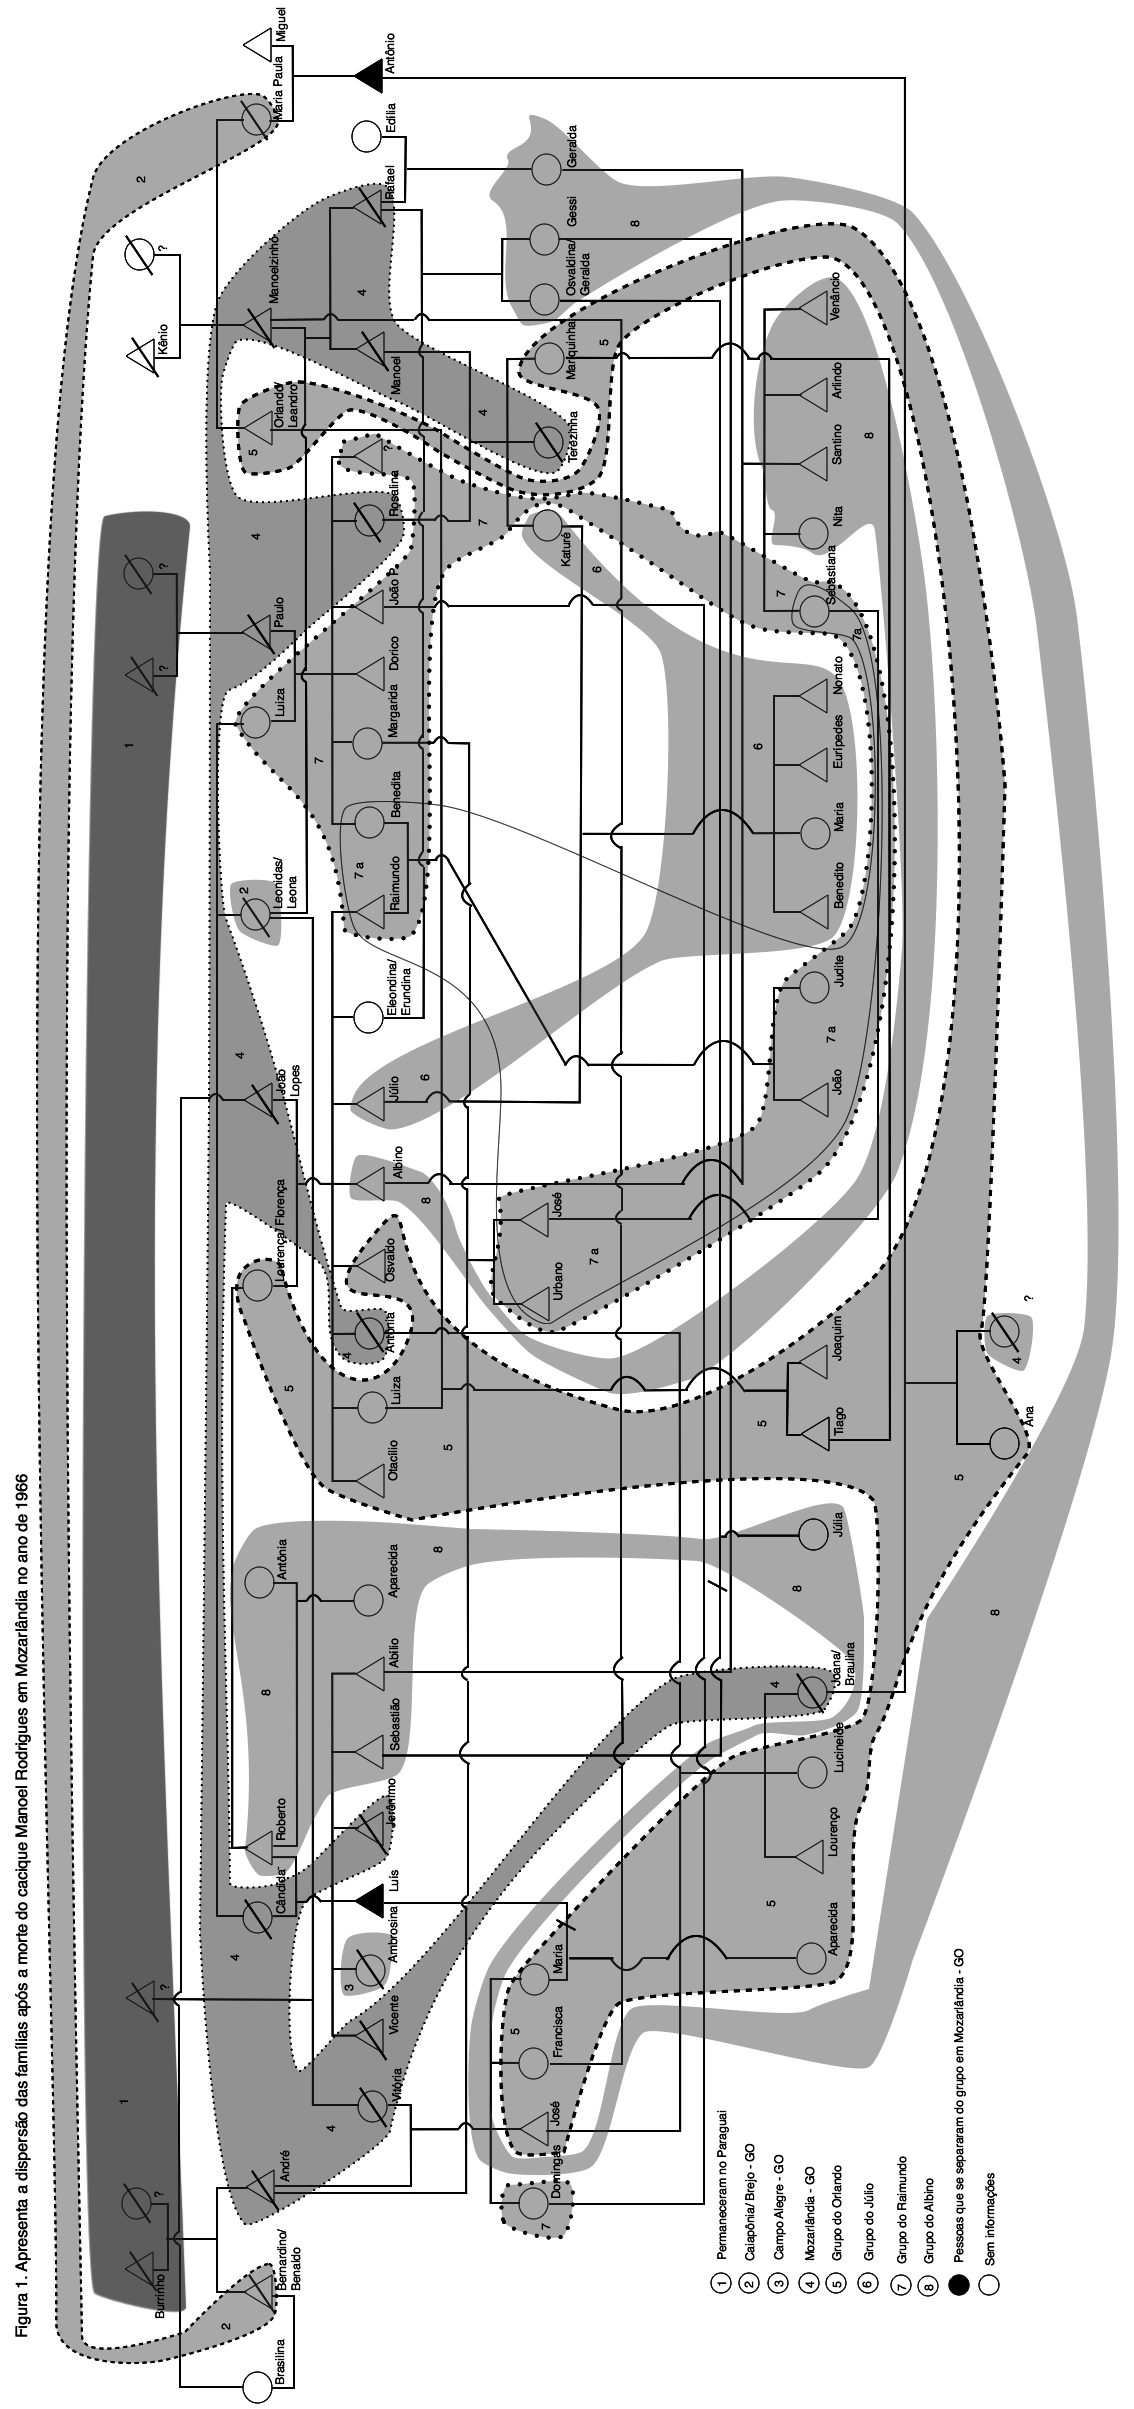
\includegraphics[width=\textwidth]{./img/GUARANIS-img9.png}

%-->IMAGEM INEXISTENTE NA PASTA, MAS EXISTENTE NO ARQUIVO .DOCX ORIGINAL! TRATAR! REMOVER LEGENDA EMBUTIDA NA IMAGEM!
%\begin{figure}
  %\centering
 %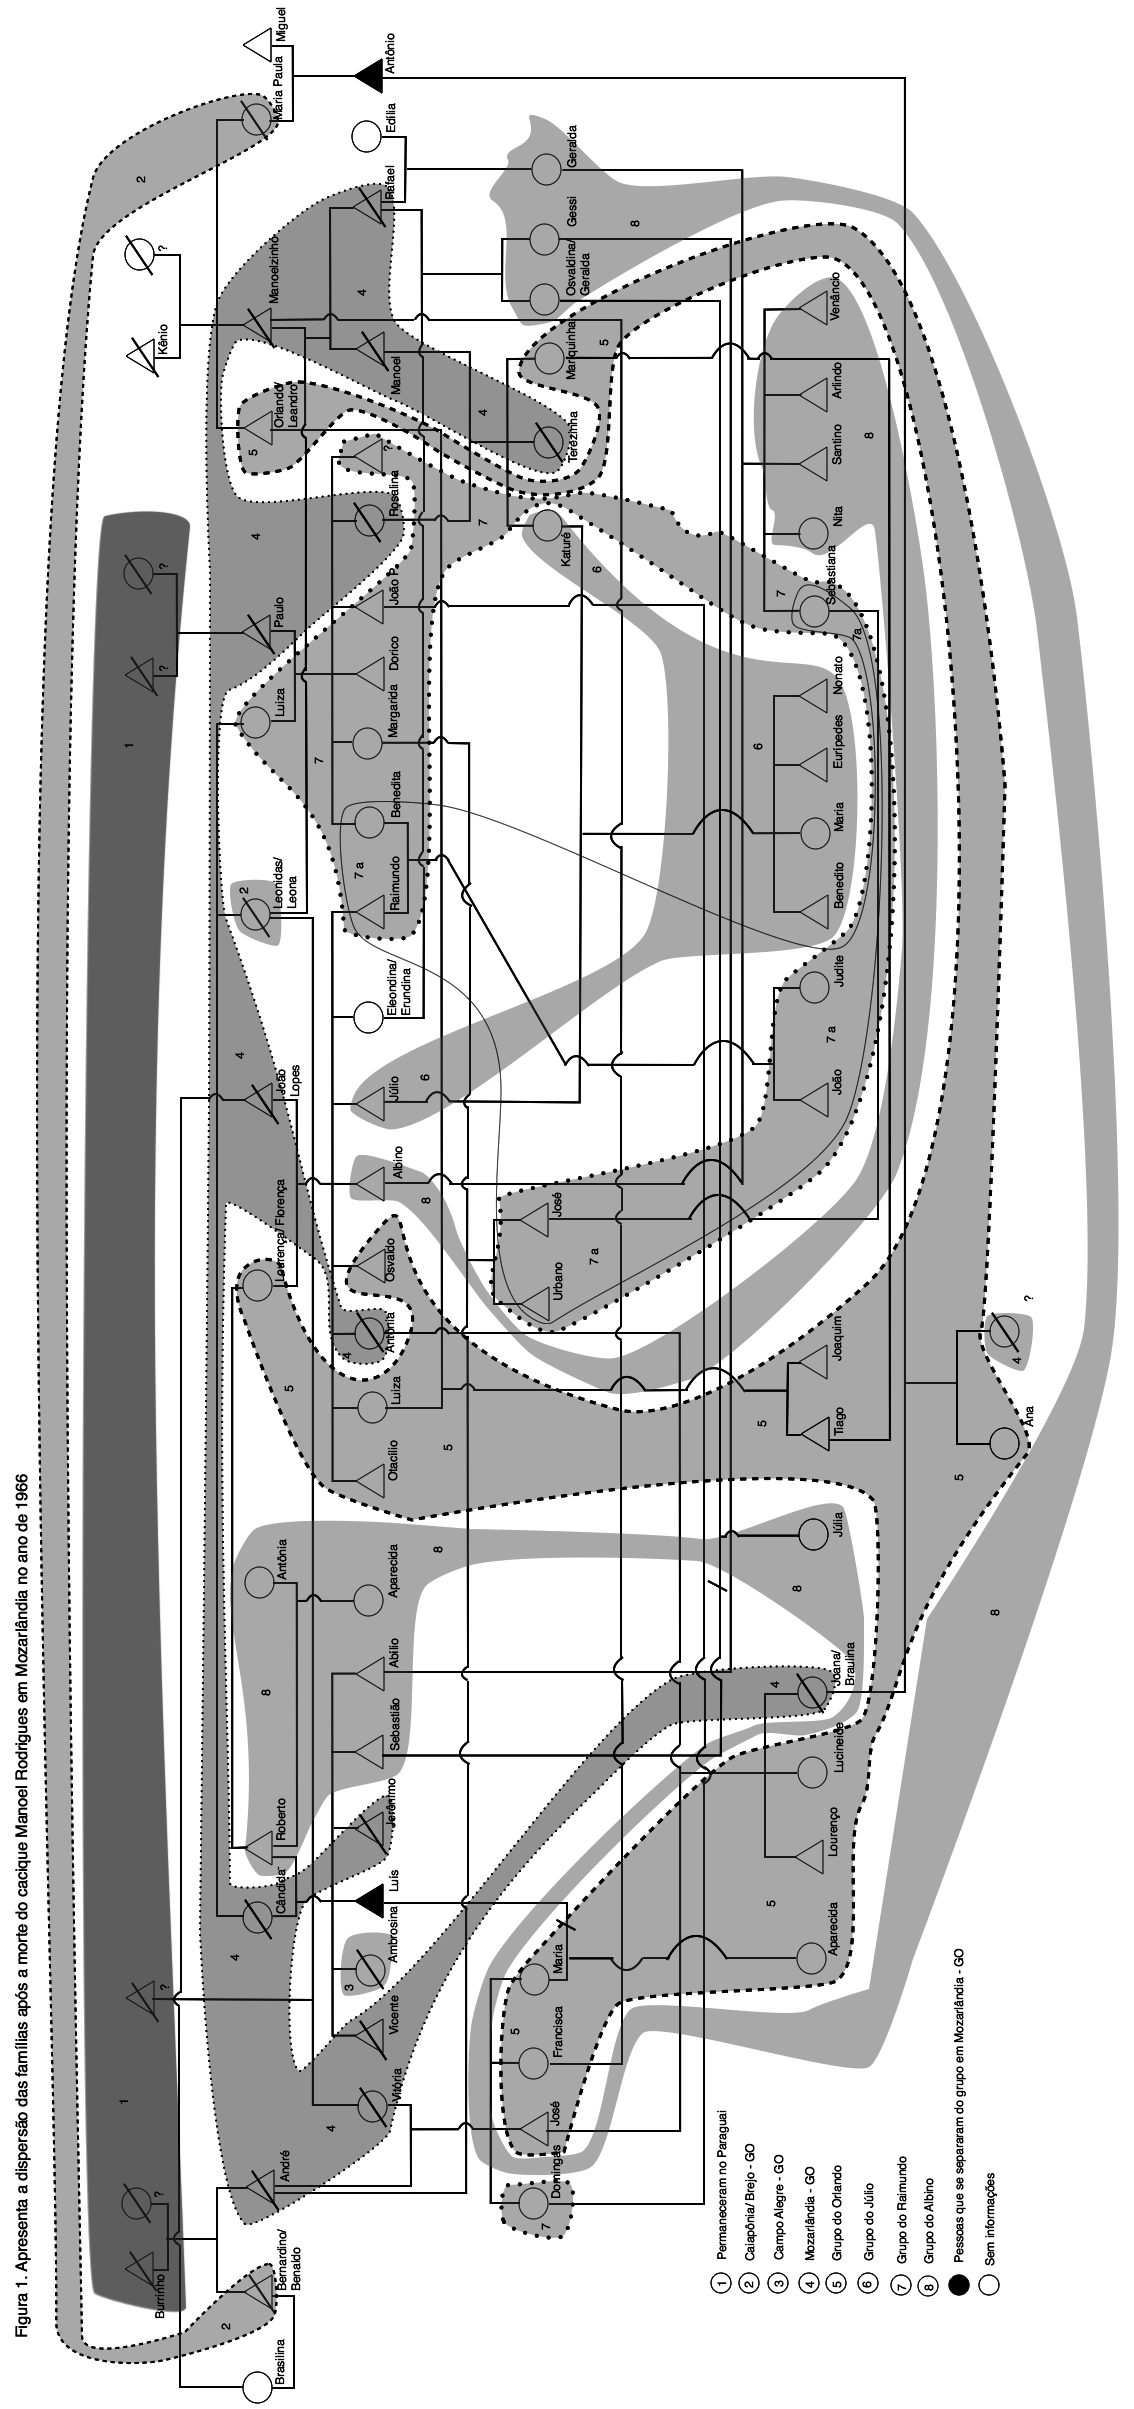
\includegraphics[width=\textwidth]{./img/GUARANIS-img9.jpg}	
  %\hfill
  %\caption{Dispersão das famílias após a morte do cacique Manoel Rodrigues em Mozarlândia (GO) no ano de 1966}
%\end{figure} 

Ao obter notícias da passagem de seus parentes, o último grupo a chegar
à Ilha do Bananal dividiu"-se e adotou estratégias diferentes. Uma parte
permaneceu na Ilha do Bananal até 1978 (sombreado 8 na figura 1); outra
parte (tracejado 7a na figura 1) seguiu o mesmo itinerário percorrido
pelo grupo de Orlando, com o qual se encontrou em fins da década de
1970.

O~reencontro ocorreu em Imperatriz e juntos viajaram até Itinga do
Maranhão. De lá foram para Castanhal, no Pará, aonde por cinco anos
trabalharam em fazendas. Nesse período, um dos filhos de Raimundo, João,
casou"-se com sua prima de segundo grau (\versal{FZDD}), Ana, com quem tem duas
filhas.

No princípio da década de 1980 os dois grupos retornaram ao Maranhão,
para a Terra Indígena Guajajara Pindaré. No diagrama 2, o sombreado
representa os grupos de Orlando e de Raimundo, no Maranhão, entre as
décadas de 1970 e 1980. Os dois grupos aumentaram consideravelmente seu
contingente populacional, no entanto, permanecia o problema da
disponibilidade de cônjuges.
%\footnote{Diferentemente do que ocorre
%entre outros povos, (Fausto, 2001), a inclusão de membros estrangeiros
%por rapto, guerra ou espontaneamente, não é comum entre os Mbya.}

%-->TRATAR! EXCLUIR LEGENDA EMBUTIDA NA IMAGEM!
\begin{figure}
  \centering
 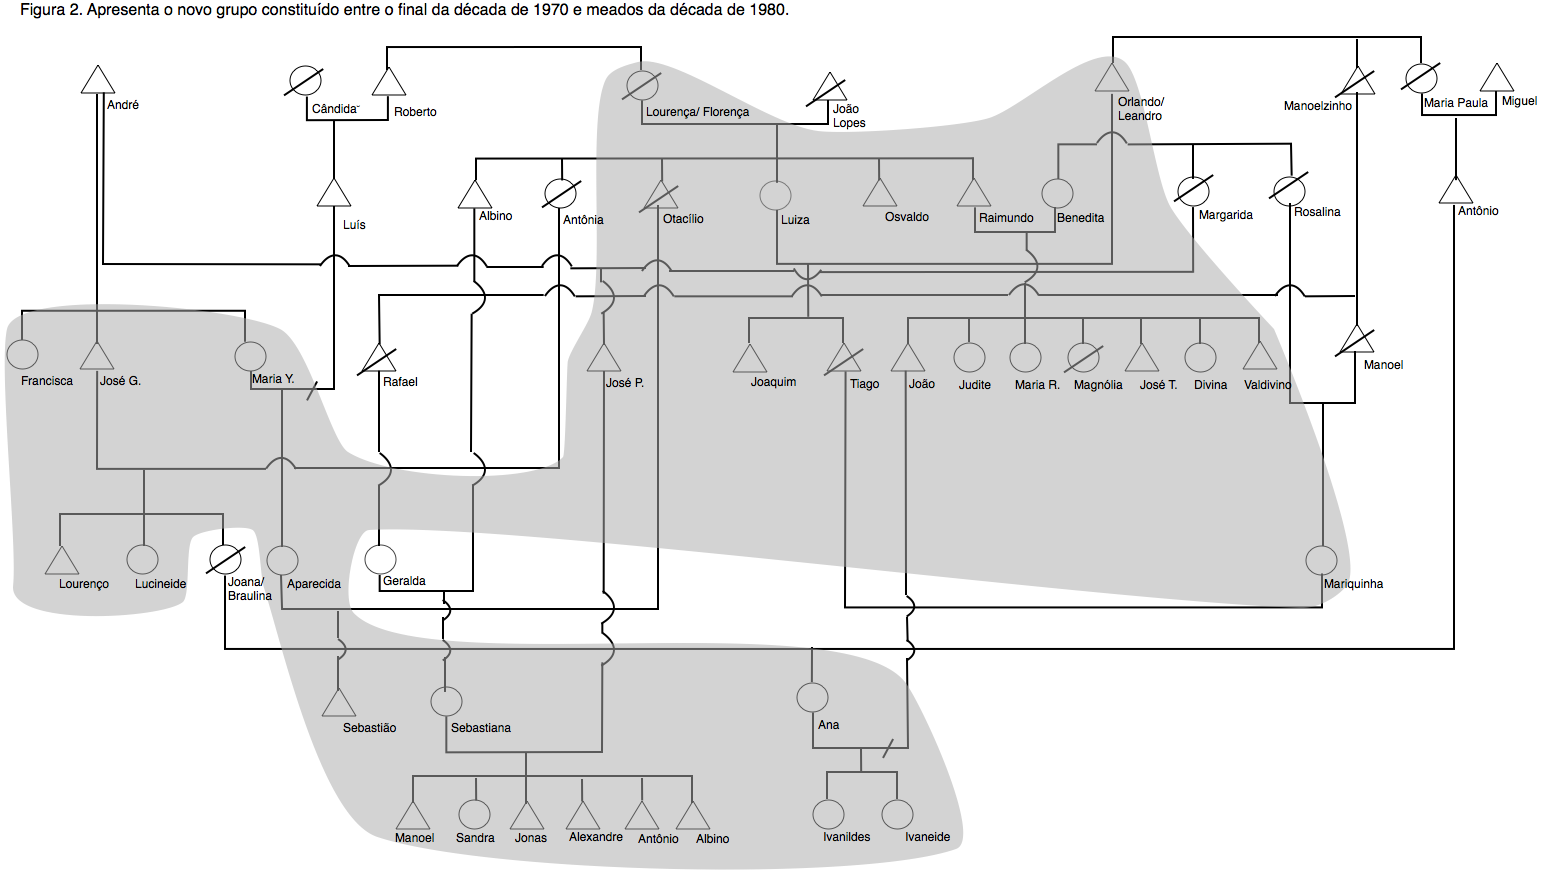
\includegraphics[width=\textwidth]{./img/GUARANIS-img10.png}	
  \hfill
  \caption{Novo grupo constituído entre o final da década de 1970 e meados da década de 1980.}
\end{figure}
 
   % Unhandled or unsupported graphics:
%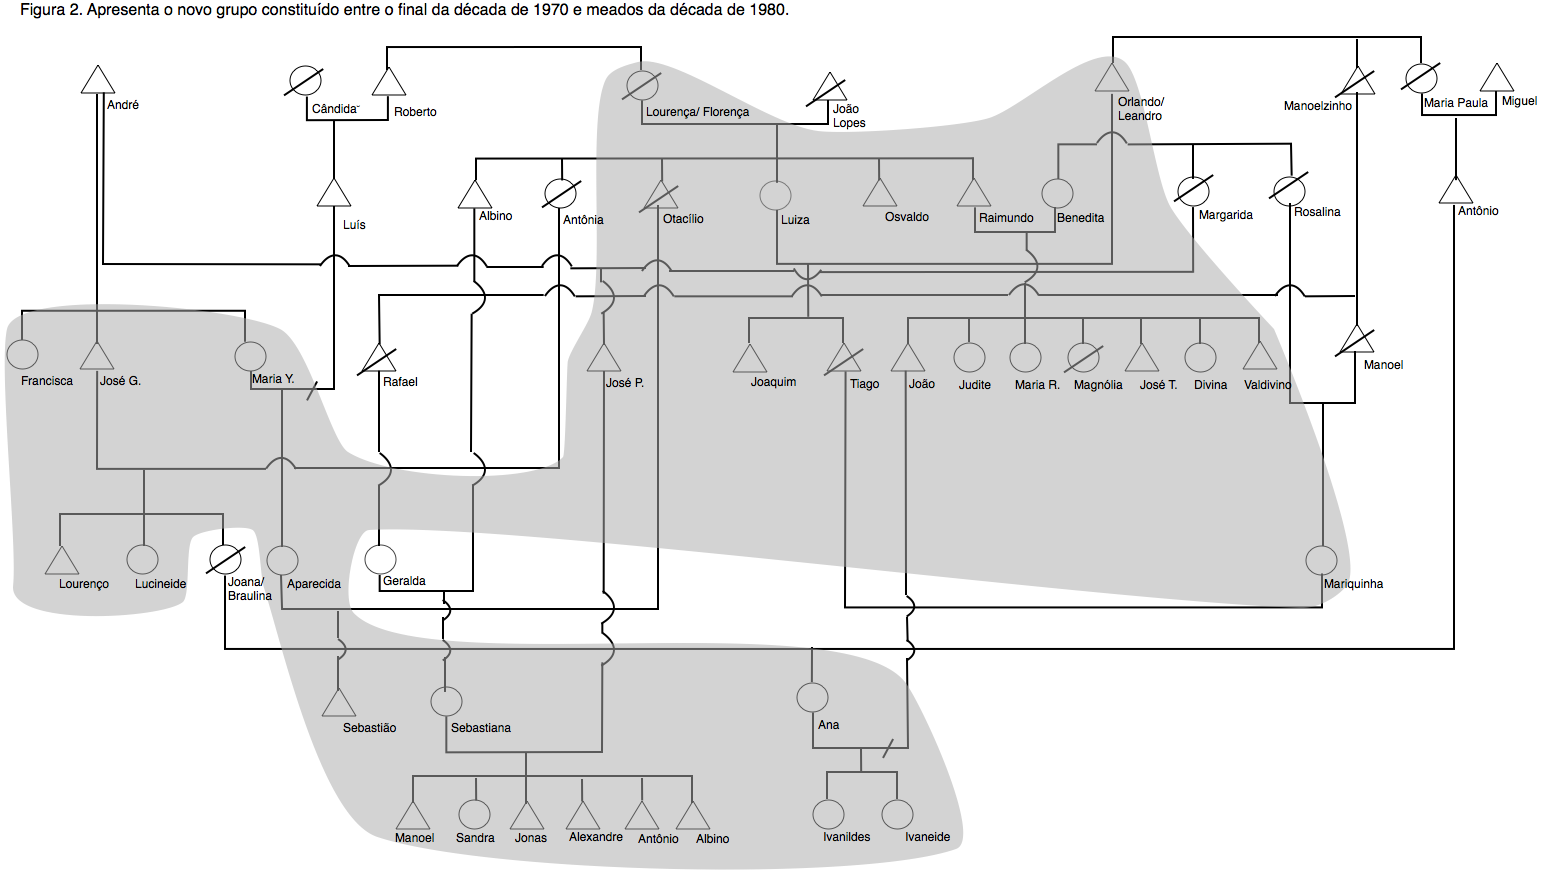
\includegraphics[width=\textwidth]{./img/GUARANIS-img10.png}
 

O~convívio com os Guajajara, a despeito de haver alguns intercasamentos,
não se constituiu de forma amistosa. À~essa animosidade acrescenta"-se a
influência de pessoas não"-índias agindo em proveito próprio junto
desses grupos
%\footnote{São inúmeros os relatos em que não índios
%invadiam as plantações dos Guarani para saquear roças ou soltavam gado
%para que pastassem em suas roças.}
e o não reconhecimento, por parte da
\versal{FUNAI}, dos Guarani como povo indígena. ``Eles diziam que nós não
podíamos ficar lá, porque éramos paraguaios'' (João Wera). 

Em meados da década de 1980, um padre chamado Carlo Bialli tomou
conhecimento da situação vivida pelos Mbya no Maranhão e gravou em uma
fita cassete a fala de um cacique da aldeia Itariri, conhecido como
Antônio Branco --- em que ele contava sobre os Guarani no Sudeste --- e
apresentou a gravação a Orlando e Raimundo, na tentativa de
convencê-los a irem para o Sudeste. Nesta época, o divórcio entre João
e Ana foi um dos motivos para que José, avô da jovem divorciada,
resolvesse aceitar a proposta do padre. Acompanhado das duas filhas, de
um tio materno, de uma irmã de Raimundo e do filho desta, o grupo
chegou ao litoral sul de São Paulo em 1987. O~filho do cacique também
aceitou a oferta do padre, indo até São Paulo e, de lá, para o Rio
Grande do Sul, de onde meses mais tarde retornou para a Terra Indígena
Mãe Maria, para onde a família de seu pai se mudou no final da década
de 1980 (ver diagrama 3).

%-->TRATAR! EXCLUIR LEGENDA EMBUTIDA NA IMAGEM!
\begin{figure}
  \centering
 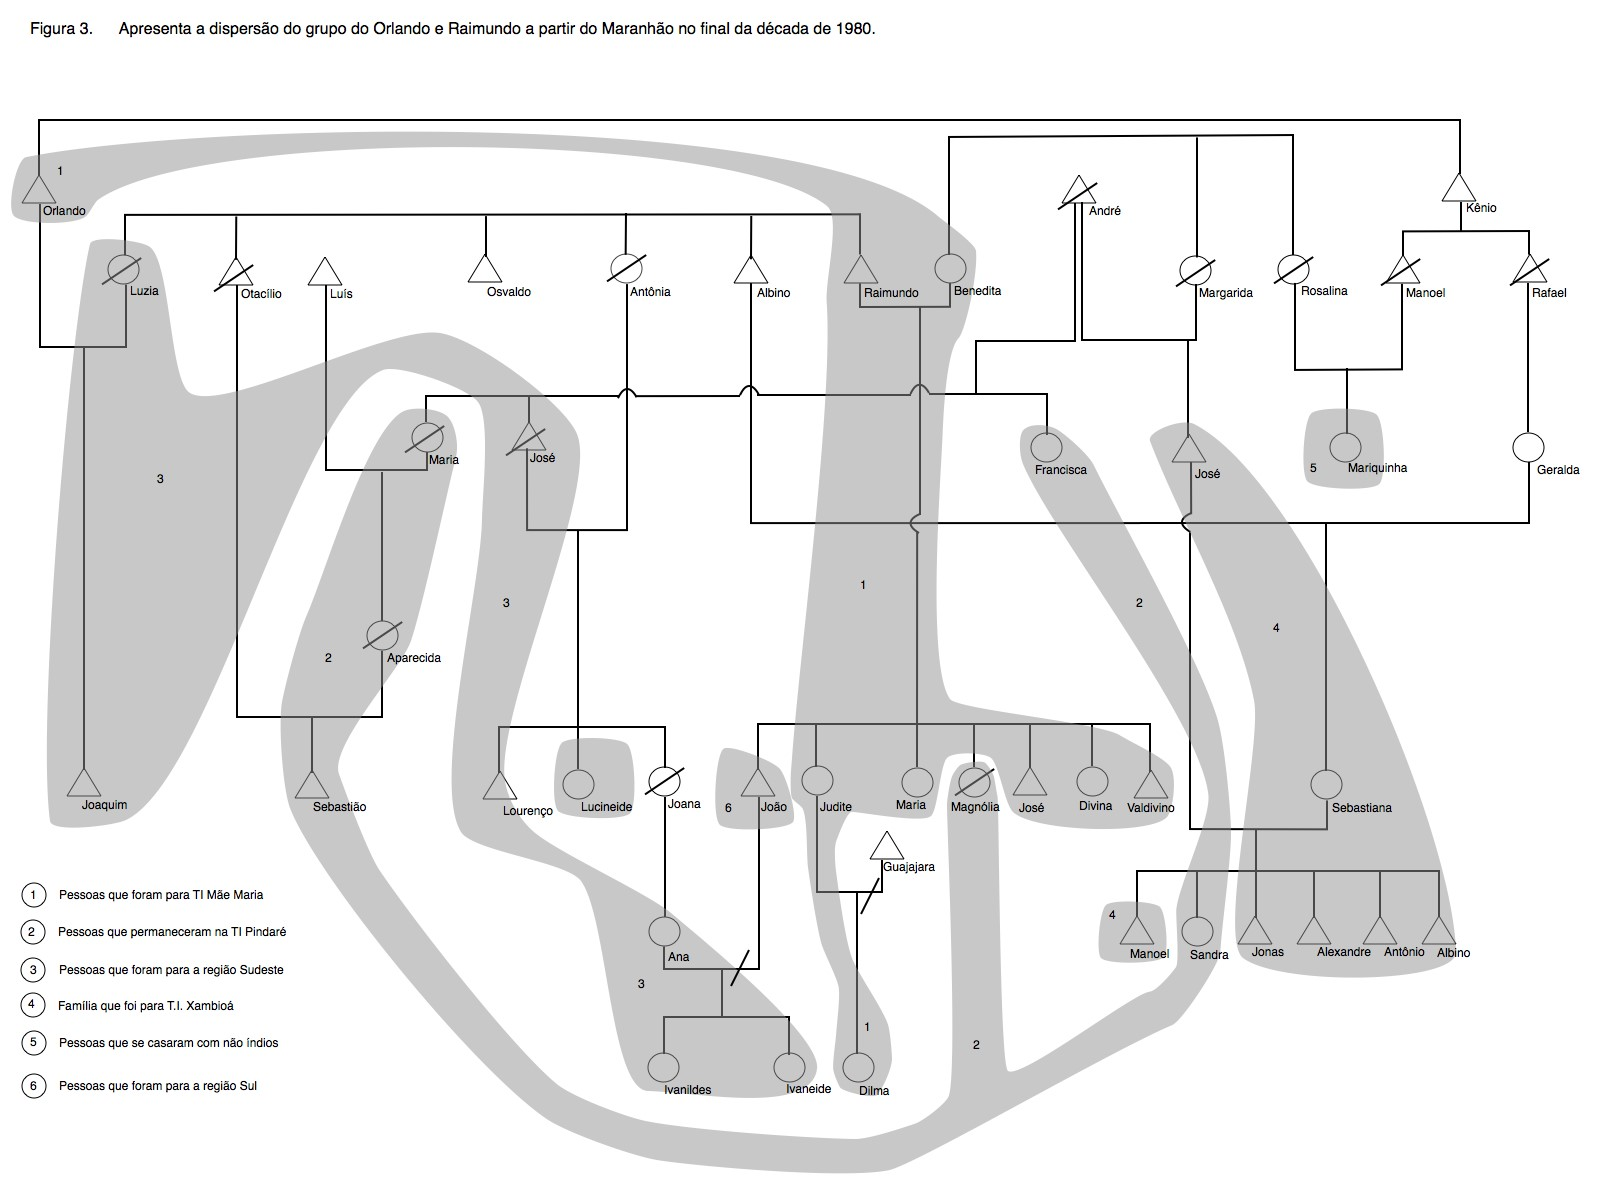
\includegraphics[width=\textwidth]{./img/GUARANIS-img11.jpg}	
  \hfill
  \caption{Dispersão do grupo de Orlando e Raimundo a partir do Maranhão no final da década de 1980.}
\end{figure}
 
   % Unhandled or unsupported graphics:
%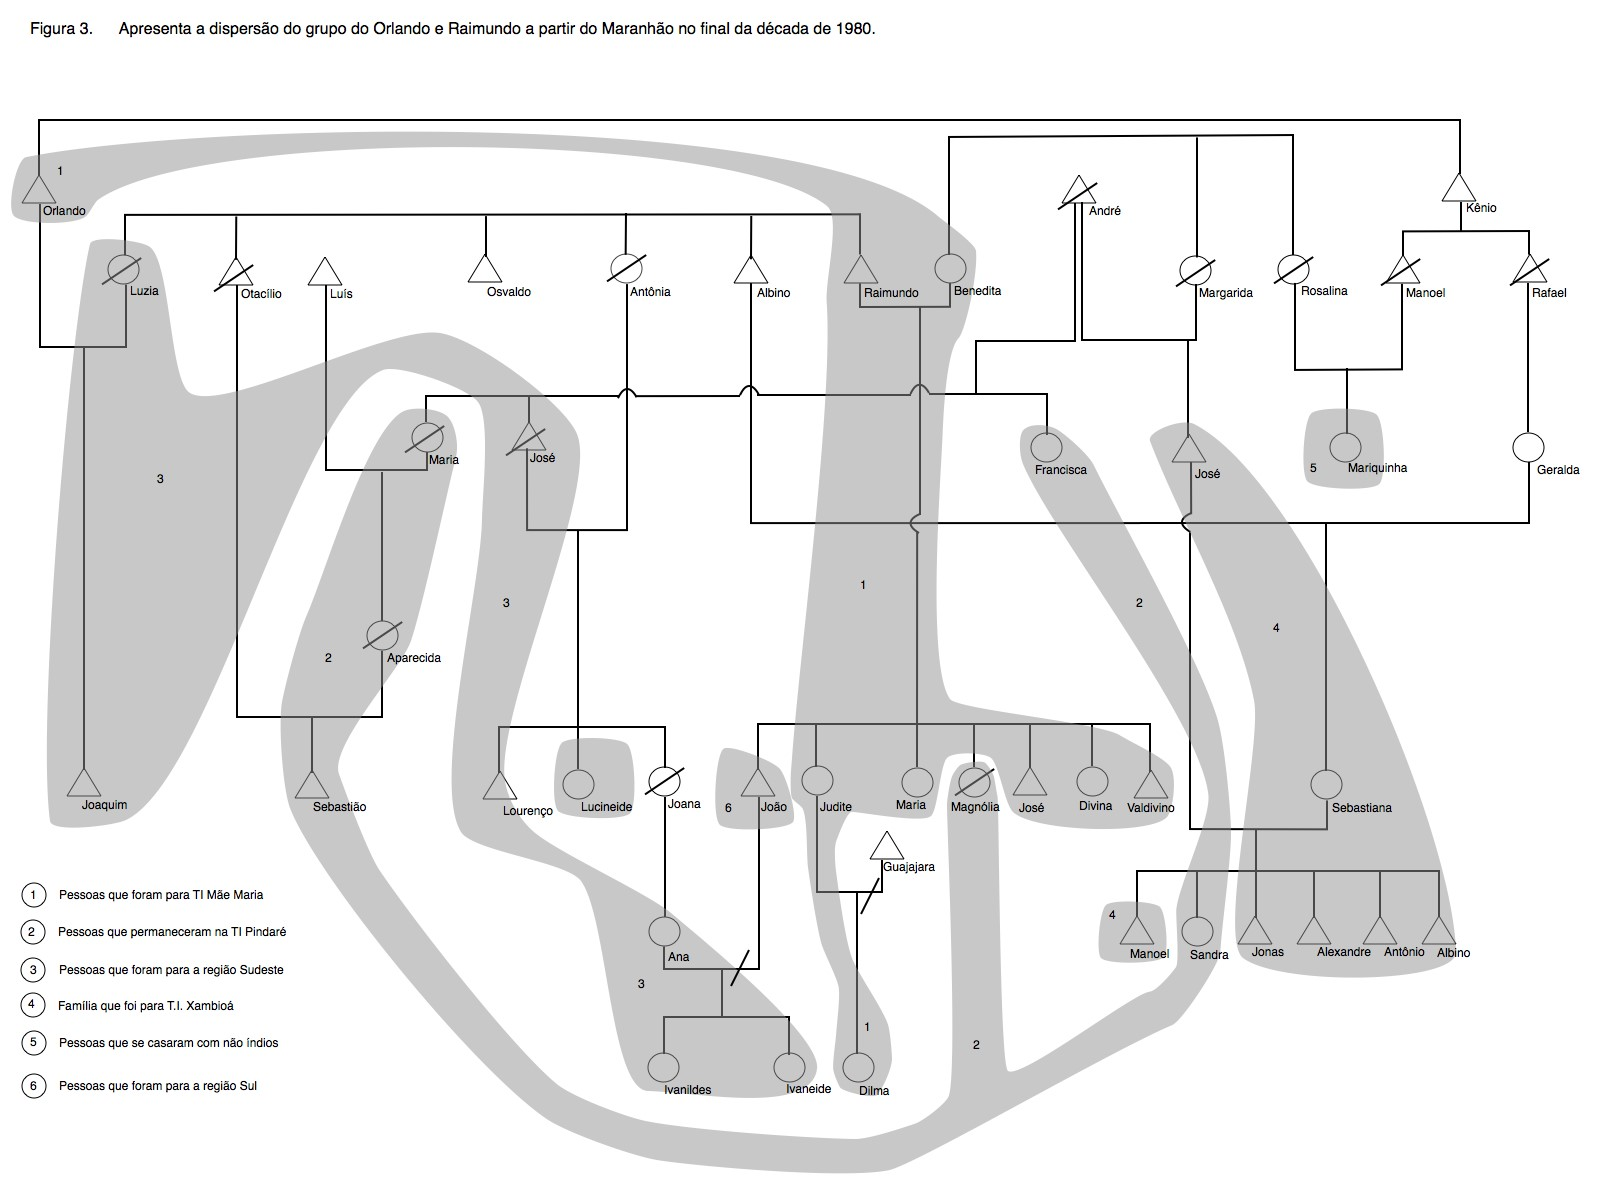
\includegraphics[width=\textwidth]{./img/GUARANIS-img11.jpg}
 

Os contextos vividos por Albino e seu grupo apresentam uma configuração
diferente. Após nove anos na Ilha do Bananal, vivendo em duas aldeias
karajá (Santa Isabel e Canoanã), no início da década de 1980 Albino se
estabeleceu com a sua família em Araguaína, onde trabalhava em
fazendas. Nesta ocasião, Maria --- que desde o início da década de 1970
vivia na Terra Indígena Xambioá --- tomou conhecimento de que seu tio
paterno estava naquela cidade e pediu ao marido que fosse buscá-lo. Em
1982, Albino e sua família chegaram a Xambioá (figura 4). 

A~convivência na aldeia dos Karajá teve duas consequências: a primeira
foram os intercasamentos. A~segunda foi a repressão por parte dos
Karajá, principalmente as crianças, em forma de zombarias e agressões
contra as crianças Mbya para que não falassem em seu próprio idioma,
mas em português, majoritariamente falado pelos Karajá naquela Terra
Indígena. O~trecho abaixo é um excerto de uma conversa mais longa junto
a Leonardo e seu tio paterno, Abílio. 

\begin{quote}
\noindent
Abílio: Meus meninos ainda falavam na linguagem\footnote{É~como os
setentrionais se referem às falas no idioma guarani.} um com o outro,
assim. Aí os outros [Karajá] ficavam rindo\ldots{} É, eles mangavam deles
aí. Então com isso aí perdeu, ficou com vergonha de falar também.

Leonardo: Foi desse jeito mesmo lá no Xambioá. Quando a gente falava na
linguagem eles jogavam pedra na gente. Jogavam pedra, mangavam, riam, é
assim mesmo. 

Abílio: Pois é, por isso que os meninos perderam, perderam não, não
querem mais falar.

Leonardo: Chegamos lá, nós conversávamos tudo na linguagem. Aí lá mesmo,
quando eu estava parando de falar na linguagem, que nós chegávamos
junto, todo mundo assim --- velho Albino, velha Geralda, tio Arlindo --- aí
eu ia conversar na linguagem e eu mesmo sorria de mim. (Abílio Karai e
Leonardo Guarany, Nova Jacundá, 24/06/2013)
\end{quote}

%-->TRATAR! EXCLUIR LEGENDA EMBUTIDA NA IMAGEM!
\begin{figure}
  \centering
 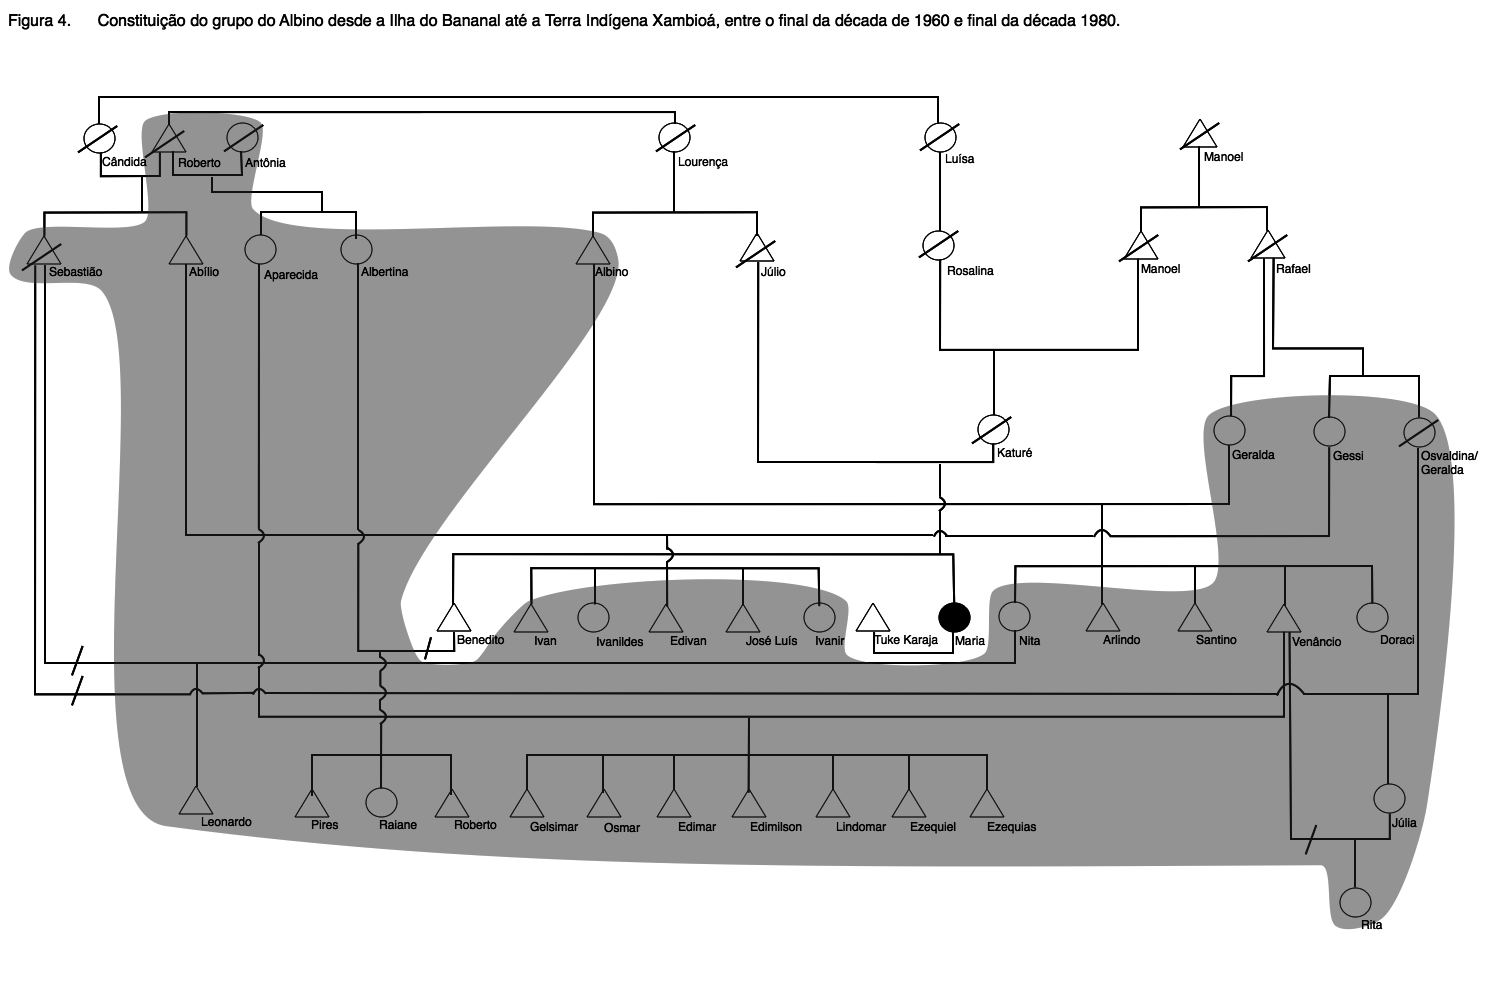
\includegraphics[width=\textwidth]{./img/GUARANIS-img12.png}	
  \hfill
  \caption{Constituição do grupo do Albino desde a Ilha do Bananal até a Terra Indígena Xambicá, entre o final da década de 1960 e o final da década de 1980.}
\end{figure}
   % Unhandled or unsupported graphics:
%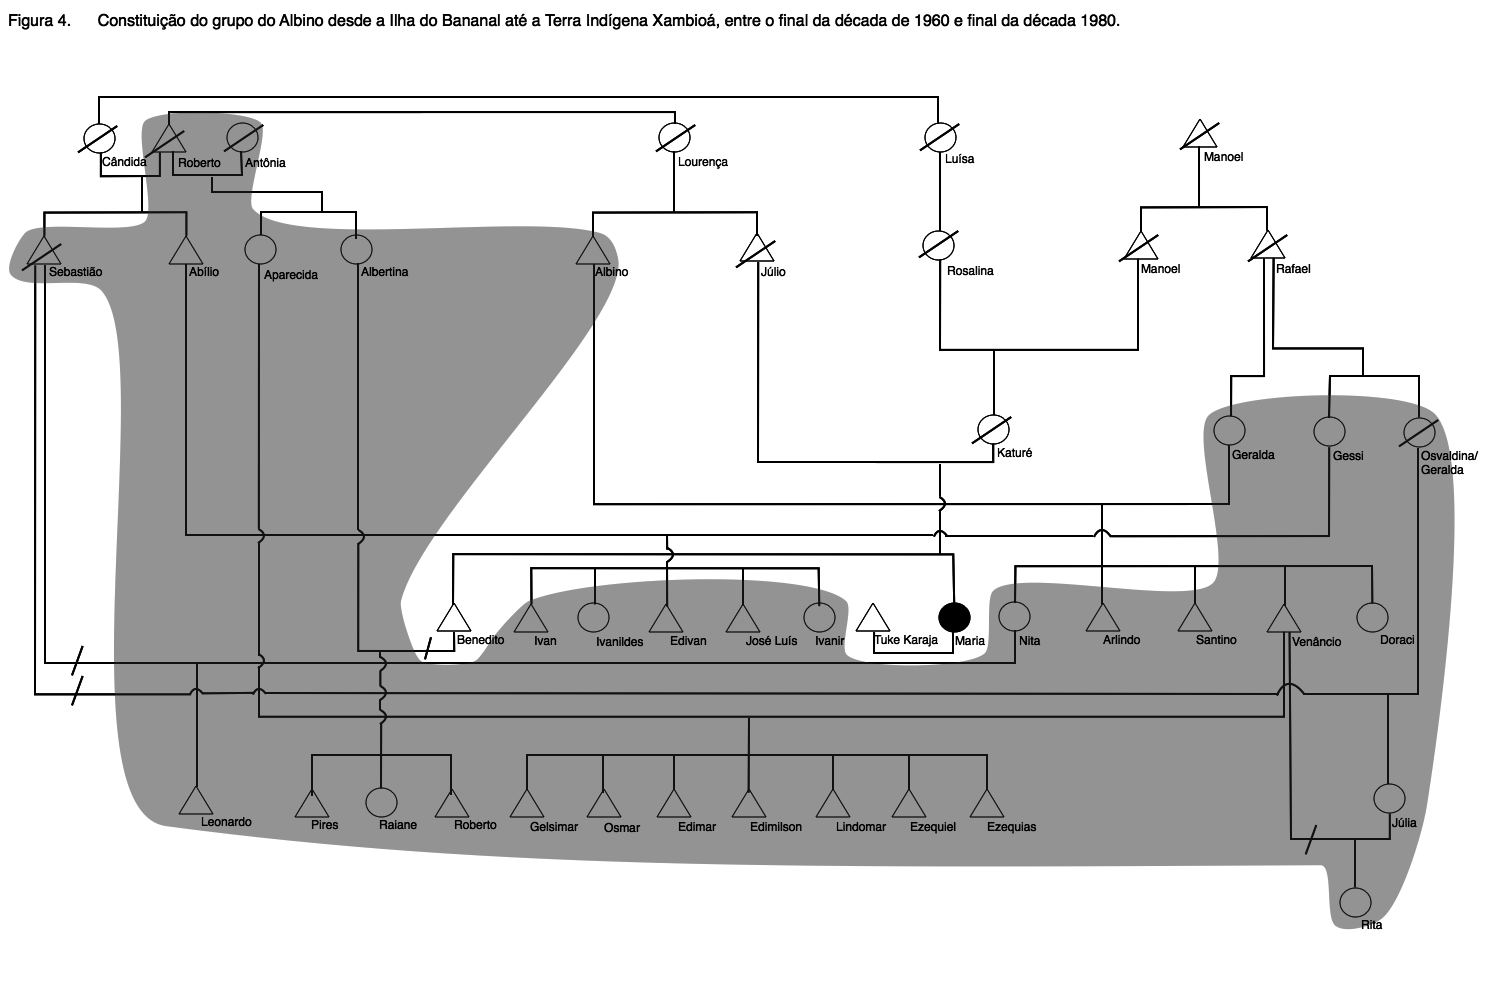
\includegraphics[width=\textwidth]{./img/GUARANIS-img12.png}
 

À~exceção da partida do primeiro grupo, liderado por Orlando, a busca
pelos parentes dispersos e o desejo de viverem juntos parecem ter sido
os principais orientadores dos deslocamentos pela região Norte. Nos
relatos anteriores, esse teria sido um dos motivos que lançaram Júlio e
Raimundo no encalço do primeiro grupo. Albino, durante anos, enviou um
de seus filhos à procura do paradeiro de seus irmãos. No entanto, foi
Eurípedes, filho de Júlio, que desde o início da década de 1970 vivia na
Terra Indígena Mãe Maria, que foi ao Maranhão levar a notícia de que
Albino estava na Terra Indígena Xambioá.

Nesta ocasião, Sebastiana manifestou o desejo de reencontrar seus pais.
Acompanhada do marido e dos filhos, no final da década de 1980 chegaram
a Xambioá, onde viveram até 1996. Como é possível observar na figura 3,
entre meados e final da década de 1980 as famílias que estavam no
Maranhão percorreram itinerários bem distintos: uma parcela (sombreado
2) casou com os Guajajara, e mais tarde outros parentes uniram"-se a ela; 
outra, sombreado 3, se mudou para o estado de São Paulo; a
família marcada com o sombreado 4 foi para Xambioá; o sombreado 1
mostra Orlando, que acompanhou a família de Raimundo até a \versal{TI} Gavião
Mãe Maria, nas proximidades de Marabá; e o sombreado 6, uma pessoa que
foi para o sul do país.

As unidades familiares, nessa ocasião bem reduzidas, se veem diante da
dificuldade de se perpetuarem de maneira endógena. Aos Mbya, que até a
chegada ao Maranhão se recusavam a contrair matrimônios com pessoas
não"-índias ou de outras etnias, impõe"-se a necessidade de abertura ao
exterior. Uma das filhas de Raimundo se casou com um homem Akewara;
outra, com um homem Gavião, e o filho mais velho foi para o Rio Grande
do Sul. 

A~convivência com os Gavião foi marcada por altos e baixos. Inicialmente
esses últimos acolheram os Mbya, interessados nas possibilidades
matrimoniais com as mulheres recém"-chegadas. Mas se tornaram hostis
diante da não efetivação plena da afinidade, seguida de um acidente que
culminou na morte de um homem Gavião durante o trabalho de abertura de
uma roça para os Mbya.

Decorrido certo tempo, as relações voltaram a se estreitar por
iniciativa dos Gavião, novamente interessados nas mulheres Mbya. A~não
celebração de alianças entre os dois grupos resultou em saques, pelos
Gavião, às roças Mbya. Diante da grave situação de conflito, Raimundo,
com ajuda da \versal{ONG} Centro de Trabalho Indigenista, adquiriu uma área de
fazenda, na qual fundaram a Terra Indígena Nova Jacundá, em 1996. O
final do período em que viveram entre os Gavião e o início da ocupação
de Nova Jacundá foi marcado por intenso estreitamento das relações
entre as pessoas que habitavam Xambioá e a família de Raimundo, após um
período de dispersão de cerca de 30 anos.

No entanto, o tempo permanecido em aldeias de outras etnias tiveram
consequências sobre os grupos futuros: a primeira foi a fixação de
cônjuges mbya nas terras indígenas Xambioá e Mãe Maria devido aos
casamentos interétnicos com os Karajá e com os Gavião. A~segunda foi o
abandono e a consequente perda do idioma. Vivendo entre grupos que
apenas algumas pessoas falavam a língua materna, as gerações mbya mais
novas se viram cerceadas de falar, no domínio público, o seu idioma. A
língua portuguesa se tornou o idioma falado majoritariamente, e o
guarani se limitou ao espaço doméstico, das gerações mais velhas entre
si e destas às mais novas. No entanto, os filhos de casamentos
interétnicos compreendem e falam apenas o idioma português. Contudo, o
reencontro das famílias em Nova Jacundá ampliou as possibilidades
matrimoniais internas e criou um núcleo mbya, que, no que se refere ao
idioma, vem alterando essas consequências.

Em 2004, poucos anos após a morte de Raimundo, alguns conflitos internos
forçaram o grupo de Albino a retornar à sua antiga sede, a Terra
Indígena Xambioá. Todavia, essa ruptura não foi absoluta e o fluxo de
pessoas mbya entre as duas aldeias continuou frequente, inclusive com
fins matrimoniais.

\section{Potencialmente afins}

A~seção anterior tratou dos deslocamentos empreendidos desde o noroeste
de Goiás até os contextos em que vivem atualmente os Mbya, por isso sua
característica mais descritiva. Nesta seção será dispensada atenção ao
problema colocado pelo reduzido número de pessoas que compunham cada
unidade em deslocamento, ampliado pelo fato de essas pessoas serem
parentes entre si.

Para os Mbya não existe uma categoria de pessoas para a qual o casamento
seja prescrito. Entre os meridionais afirma"-se que uma pessoa deve
casar com alguém que não seja classificado como parente, categoria que
inclui os tios e tias maternos e paternos, os primos cruzados e
paralelos e os filhos e filhas de irmãos e irmãs reais de ego.
Indiretamente, a categoria parente pode incluir qualquer pessoa que
esteja relacionada por cognação a uma das categorias anteriores, mas
esses são classificados como parentes distantes e o casamento entre
tais pessoas, embora criticado, não é raro\footnote{É~necessário
destacar aqui uma distinção entre parentes, de um lado, e consanguíneos
e afins, de outro. As categorias nativas que traduzimos por parente ---
\emph{xeretarã} ou \emph{xeregua’i} --- possuem, para os Mbya, um campo semântico
vasto, podendo ser aplicadas desde pessoas com vínculos cognáticos até
os demais concidadãos, fenômeno recorrente entre os ameríndios
(Riviére, 2001; Vilaça, 1992; Pissolato, 2007; Mello, 2006; Silva,
2009).}. 

``Aqui nós casamos com primos de segundo grau'', afirmou"-me uma mulher com
quem eu conversava em Nova Jacundá. Este tipo de casamento, oblíquo,
revela, para o contexto Mbya, uma característica comum a outros
contextos amazônicos, como entre os Parakanã, por exemplo, (Fausto,
1991; 2001). Porém, diferentemente destes últimos, os casamentos não
são entre irmão da mãe e filha da irmã (\versal{MB}/\versal{ZD}), modelo clássico do
avunculato amazônico. Entre os Mbya, não é o irmão da mãe que é
convertido em genro de sua própria irmã, mas o primo ou primos cruzados
ou paralelos que, classificado como irmão ou irmã, é transformado em
genro ou nora. Diferentemente do caso Parakanã, não é uma relação entre
tios e sobrinhas (Fausto, 1995), mas entre pessoas que são
classificadas como avôs e netas. Os Mbya setentrionais classificam os
filhos de irmãos classificatórios não necessariamente como sobrinhos,
mas como netos.

Dos oito casamentos atuais em Nova Jacundá, quatro se deram entre
pessoas relacionadas segundo as classes acima. Em Xambioá são dois
casos, e se retrocedermos um pouco mais no tempo, encontraremos este
modelo de casamento. Tudo se passa como se os Mbya incluíssem no polo
da afinidade virtual todas as pessoas que não pertençam às categorias
acima.

Entre os Mbya meridionais, não é raro encontrarmos esse tipo de
casamento, porém tal como em Xambioá, onde o menu é mais variado, os
arranjos conjugais também podem sê-lo. O~que se conclui é que para os
Mbya são interditas as categorias pai, mãe, irmão, irmã, tio, tia
maternos e paternos, e primos e primas de primeiro grau. Esse ponto foi
explicitamente enunciado, em português, pelo cacique quando manifestava
preocupação por não haver cônjuges disponíveis em Nova Jacundá. As
mulheres citadas no trecho abaixo são as suas irmãs reais.

Eu fico preocupado porque daqui a pouco nós vamos acabar, porque vai ter
que casar com jurua ou com outros índios; então é melhor casar com
outros índios, porque aqui não tem com quem casar. Vê os meus filhos,
com quem eles vão se casar? Com as filhas da Maria? Da Divina? E~elas
com quem vão casar? Não pode! Nós somos índios, mas não somos bichos
não, a gente sabe que é errado!'' (João Wera, Nova Jacundá, 11/06/2012).

Em sua tese de doutorado, Mello (2006: 75) havia chamado a atenção para
esse ponto: o incesto ``considerado como uma conduta animalesca, é
tratado com certo constrangimento''. No trecho acima, a conduta
incestuosa é o casamento entre os primos de primeiro grau. Destaco que
os Mbya, formalmente, não distinguem entre primos paralelos e primos
cruzados; isso não significa que as noções de consanguinidade e de
afinidade não constituam modelos relacionais no socius mbya, elas serão
acionadas ou negadas conforme o campo relacional em jogo: a afinidade
amazônica, citando Viveiros de Castro, ``não só determinam outros
referentes que os nossos, como envolvem outros componentes'' (2002: 406).
Na sequência reitera: a afinidade pode se aplicar a relações com
estranhos, mesmo se nenhum casamento acontece; e mais, ela se aplica
sobretudo àqueles casamentos com os quais o casamento não é uma
possibilidade pertinente'' (idem: 408).

Esse problema da pertinência ou não de certos casamentos é fundamental.
É~conhecido na literatura antropológica histórias de pessoas que,
seduzidas por membros de outras espécies, terminam por irem residir no
mundo dessas pessoas como afins (Vilaça, 1992, 2005; Lima, 1996). Esse
tipo de transformação não é estranha aos Guarani, que a denominam
jepota. Como em outros contextos ameríndios, ocorre quando uma pessoa,
em determinadas fases da vida, é seduzida por um membro de uma espécie
animal e passa a tomá-lo como parceiro sexual (Clastres, 1978; Macedo,
2013; Mendes Júnior, 2009; Pissolato, 2007; Schaden, 1962 [1954]).

Outro modelo de casamento impertinente é aquele que se estabelece entre
pessoas Mbya e não"-Mbya (\emph{jurua} ou \emph{te’yi}). Este tipo de casamento é
denominado, entre os setentrionais, \emph{jejavy}\footnote{\emph{Javy} tem o
significado de pecar, errar, ou equivocar (Cadogan, 1992). \emph{Jejavy},
entre os setentrionais, possui este significado preciso: casar"-se com
pessoas não"-mbya. Migliora (2014) e Pereira (2014) abordam os
casamentos entre Mbya e \emph{jurua} de uma forma positiva a partir de suas
experiências de campo na aldeia das Sementes, \emph{tekoa} Mbo’y ty, em
Niterói.}. No entanto, \emph{jejavy} não se restringe apenas ao casamento, mas
a qualquer tipo de relação sexual entre essas pessoas. O~motivo de sua
impertinência é o enfraquecimento do espírito (\emph{nhe’ë}) dos pais causado
pela mistura de sangue através da relação sexual. Os filhos desses
casamentos, entre os setentrionais, não eram nominados\footnote{Durante
a construção das genealogias, apontaram"-me três pessoas que não
possuíam nomes mbya. O~motivo era claro: ``\emph{jurua ra’y ou jurua rajy}''
(filho ou filha de pai \emph{jurua}).} pelo xamã, restando"-lhes apenas o nome
brasileiro. Esse enfraquecimento, no limite, ocasiona a morte da
pessoa.

\emph{Jejavy} e \emph{jepota} são, portanto, dois modos indesejados de relação com o
exterior e pela mesma razão: a perda da verdadeira condição humana.
A~vítima de jepota deixa o convívio de seus parentes e termina por
viver entre os animais. A~vítima de jejavy também deixa o convívio de
seus parentes, não ensina o seu idioma aos seus filhos e termina por
viver como \emph{jurua} ou \emph{te’yi}, entre brancos ou índios. 

\section{Novos encontros, novos contextos}

O~objetivo dessa seção é percorrer os fios que conectam as aldeias
setentrionais às meridionais, em especial Parati"-Mirim e Araponga,
localizadas no município de Parati, no estado do Rio de Janeiro. Vimos
no diagrama 3 que as pessoas no sombreado 3 seguiram para os estados da
região Sudeste. O~que motivou essas pessoas a deixar o convívio junto
de seus parentes para seguir em direção a terras e pessoas que, embora
guarani, eram estranhas?

Como mostrei na segunda seção, os Mbya enfrentavam uma convivência
difícil entre os Guajajara. Neste mesmo período, uma mulher havia se
separado recentemente de seu marido e, segundo relatos, não havia com
quem se casar que não fosse guajajara ou \emph{jurua}. Essa época coincidiu
com a oferta do padre Bialli para que as pessoas aceitassem a proposta
de se mudarem para São Paulo. Acompanhada de seu tio materno, Ana, suas
duas filhas, e mais duas pessoas (cf. figura 3) aceitaram a oferta e
entre meados e o final da década de 1980 chegaram ao Itariri.

Lá encontraram um grupo que recentemente deixara o oeste do Paraná e
seguia em direção ao litoral. A~convivência conjunta teve como
resultado o casamento entre Ana e um dos rapazes do grupo. Certo tempo
se passou até que o novo grupo seguiu para o Espírito Santo. As demais
pessoas que vieram do Pará permaneceram por um tempo no Itariri e, mais
tarde, o tio materno de Ana foi para a aldeia Krukutu, onde
reencontraria seu pai. Do Espírito Santo o primeiro grupo se mudou para
duas aldeias no estado do Rio de Janeiro e posteriormente fundaram a
aldeia Parati"-Mirim, em meados da década de 1990.

O~que afirmou Pissolato para os Mbya meridionais não é menos plausível
para os setentrionais: ``[\ldots{}] a movimentação de pessoas é em si o modo
de realização do parentesco [\ldots{}] e a expressão da atitude mais
fundamental da busca pessoal de satisfação'' (2007: 59); ``se não se fica
alegre entre parentes, deve"-se deixá-los para buscar parentes outros''
(idem).

Paralelamente à partida do primeiro grupo, João, o ex"-marido da jovem,
deixou a sua família e seguiu em direção ao Sudeste. Num primeiro
momento seguiu de Angra dos Reis até o Rio Grande do Sul, de onde
retornou a Marabá. Mais tarde, acompanhado de José, o avô de sua
ex"-esposa, e de um primo seu chegou a São Paulo, onde os deixou e
seguiu novamente para o Rio Grande do Sul. Em Porto Alegre conheceu
algumas pessoas da aldeia Pacheca, localizada no extremo sul do estado,
que o convidaram para ir até lá. Pouco após sua chegada a essa aldeia,
casou"-se com uma jovem e, em seguida, convenceu a família de sua esposa
a acompanhá-lo até o Rio de Janeiro, onde se encontravam alguns
parentes de seu sogro.

No princípio da década de 1990, chegaram a Angra dos Reis, e mais tarde
a Ubatuba. Nesta última aldeia deixou sua mulher grávida e partiu para
a aldeia Rio Branco, no estado de São Paulo, onde se casaria novamente
e teria outro filho. O~grupo que deixara em Ubatuba se estabeleceu, em
meados da década de 1990, na aldeia Araponga, no sul do Rio de Janeiro.
Após cinco anos na aldeia Rio Branco, este homem decidiu retornar ao
Pará, indo para a terra que finalmente pertencia aos seus parentes.

A~análise de Pissolato atinge aqui sua importância comparativa. Do ponto
de vista das pessoas envolvidas, a permanência na região Norte
representava um quadro desfavorável ao estabelecimento de novas
alianças de parentesco, visto que as oportunidades eram restritas. A
busca de outros contextos que possibilitassem a realização do
parentesco despontava como objetivo pessoal de satisfação. A~recusa em
incorrer em \emph{jejavy}, casamentos cujas possibilidades não são
pertinentes, motivou esses núcleos a caminhar; ou como colocou a
autora, a buscar parentes outros. 

A~fixação de famílias em Parati"-Mirim, bem como o nascimento de filhos
em Araponga e Rio Branco, conecta as aldeias setentrionais e
meridionais. O~fluxo de pessoas entre elas não é tão intenso quanto é
entre as aldeias meridionais, porém existe. Mais intenso é a circulação
de notícias e o desejo de fazer com que os de um lado saibam o que
ocorre do outro lado. A~distância entre as duas regiões talvez seja, na
atualidade, a maior dificuldade para essa circulação de pessoas. Aquele
que se desloca, ao mesmo tempo que deseja buscar a satisfação de novas
possibilidades de parentesco, lamenta"-se por deixar os parentes. 

Ter ou não parentes em um lugar é sempre posto em evidência durante as
situações de conflito. Em 2007, o cacique de Nova Jacundá foi até
Parati"-Mirim com o objetivo de levar pessoas para a sua aldeia.
Acompanharam"-no uma família cujo marido era primo do cacique, e a
sobrinha da esposa deste primo. A~saudade que a mulher deste primo
sentia de seus parentes (\emph{ndovy’ai}), a morte de dois filhos
recém"-nascidos e a diferença de contextos entre as duas regiões foram
fatores decisivos para que essa família voltasse para o Sudeste. No
entanto, a sobrinha, que se casara com um rapaz em Nova Jacundá,
permaneceu. Com o passar do tempo, a saudade de seus parentes e alguns
conflitos com seus afins trouxeram"-na de volta à aldeia Krukutu, em São
Paulo.

\section{Nota Final}

Ao longo deste artigo procurei mostrar como se configura o contexto
etnográfico dos Mbya no norte do Brasil. Nesse esforço, destaquei dois
temas clássicos tanto na antropologia em geral como na etnografia dos
povos guarani: o parentesco e a busca da Terra sem Mal. Acompanhar os
movimentos migratórios e a mobilidade nessas regiões significou
percorrer os fios de uma complexa rede de parentesco, sem o que
corremos o risco de enxergar os Mbya como pequenas ilhas num oceano de
etnias.

O~caso setentrional revelou"-se conspícuo no que se refere ao estudo do
parentesco, principalmente quando comparados a outros modelos
amazônicos; penso aqui nos desenvolvimentos trazidos por Viveiros de
Castro (1993; 1996; 2002); Lima (1996) e Vilaça (2005), excelentes
ferramentas para analisarmos o tema da afinidade justamente ali onde
ela existe como potência --- \emph{jepota} e \emph{jejavy}. Paralelamente, este
contexto torna visível uma forma matrimonial menos perceptível entre os
meridionais: o casamento oblíquo entre primos de segundo grau.

Ao longo deste trabalho o termo migração gozou do mesmo estatuto que
lhes deram Nimuendaju (1987 [1914]), Clastres (1978 [1975]) e Schaden
(1962 [1954]): o deslocamento de um grupo de pessoas conduzido por um
xamã em busca da Terra sem Mal. Sendo assim, o período de migração está
compreendido entre a saída do Paraguai, na década de 1930 e a morte do
segundo xamã, em meados da década de 1960, em Goiás.

Aos deslocamentos para a ``visitação entre parentes, busca por cônjuges e
outra diversidade de motivos implicados nos movimentos populacionais do
grupo'' mantenho o termo proposto por Garlet: mobilidade (Garlet, 1997:
16 \emph{apud} Pissolato, 2007: 97). Após o falecimento do xamã, o
esfacelamento e a dispersão do grupo ao longo do interflúvio
Araguaia"-Tocantins possui uma característica ambígua. Inicialmente
oscila entre a busca da terra sem mal e a procura por parentes,
afirmando cada vez mais essa última característica. 

Diante disso, diferentemente de Garlet, que classifica as migrações como
variantes da mobilidade, neste trabalho os dois termos deverão ser
mantidos em separado. Essa opção se justifica pelo fato da mobilidade,
como acima definida, dar"-se entre territórios guarani. As diversas
terras indígenas guarani existentes ao longo das regiões Sul e Sudeste
do Brasil, entre as quais é possível observar relações de parentesco
pré-estabelecidas que muitas das vezes orientam os deslocamentos de
pessoas ou grupos. Diferentemente, os Guarani que se deslocaram em
direção à região Norte foram orientados pelo desejo de se chegar à
Terra sem Mal, localizada na direção do sol nascente, não contando,
portanto, com nenhuma rede de parentesco ou de outras relações
quaisquer pré-estabelecidas.

\section{Referências}

\begin{Parskip}
\versal{ALBERNAZ}, Adriana. \emph{Antropologia, histórias e
temporalidades entre os Ava"-Guarani de Oco’i (\versal{PR})}. Tese de Doutorado.
\versal{UFSC}, 2009.

\versal{CADOGAN}, Leon. \emph{Dicionario mbya"-guarani"-castellano}. Asunción: Ceaduc"-
Cepag, 1992.

\versal{CAPDEVILA}, Luc. ``La guerre du Chaco Tierra adentro déconstruire la
representation d’un conflit international''. In: Capdevila, Luc;
Combès, Isabelle; Richard, Nicolas; Barbosa, Pablo. \emph{Les
hommes transparents: indiens et militaires dans la guerre du Chaco
(1932-1935)}. Rennes: \versal{PUR}, 2010.

\versal{CHAMORRO}, Graciela. \emph{A~espiritualidade guarani: uma teologia ameríndia
da palavra}. São Leopoldo: Ed. Sinodal, 1998.

\versal{CLASTRES}, Hélène. \emph{A~terra sem mal: o profetismo tupi"-guarani}. São Paulo:
Brasiliense, 1978.

\versal{FAUSTO}, Carlos. \emph{Os Parakanã. Parentesco e avunculato}. Dissertação de
Mestrado. \versal{PPGAS}-\versal{UFRJ}, 1991.

\_\_\_\_. ``De primos e sobrinhas: terminologia e aliança entre os Parakanã
(Tupi) do Pará''. In: Viveiros de Castro, Eduardo (org.). \emph{Antropologia do
parentesco: estudos ameríndios}. Rio de Janeiro: \versal{UFRJ}, 1995.

\_\_\_\_. \emph{Inimigos Fiéis}. São Paulo: Edusp, 2001.

\versal{HEURICH}, Guilherme. \emph{Outras alegrias: parentesco e festas mbya}.
 Dissertação de Mestrado. \versal{PPGAS}-Museu Nacional, 2011.

\versal{LADEIRA}, Maria Inês. \emph{O~caminhar sobre a luz: o território mbyá à beira
do oceano}. Dissertação de Mestrado. \versal{PUC}-\versal{SP}, 1992.

\_\_\_\_. \emph{Espaço geográfico guarani"-mbya: Significado,
constituição e uso}. São Paulo: Edusp, 2008.

\versal{LIMA}, Tânia Stolze. ``O~dois e seu múltiplo: reflexões sobre o
perspectivismo em uma cosmologia tupi''. \emph{Mana}, vol.~2, n.~2, 1996.

\versal{MACEDO}, Valéria. \emph{Nexos da diferença. Cultura e afecção em uma aldeia
guarani na Serra do Mar}. Tese de Doutorado. \versal{PPGAS}-\versal{USP}, 2009.

\_\_\_\_. ``De Encontros nos Corpos Guarani''. \emph{Ilha}, vol.~15, n.~2, 2013.

\versal{MELIÀ}, Bartolomeu. \emph{El Guarani: experiencia religiosa}. Asunción:
Ceaduc"-Cepag, 1991

\versal{MELLO}, Flávia. \emph{Aetchá Nhaderukuery karai retarã: Entre
deuses e animais: xamanismo, parentesco e transformação entre os
Chiripá e Mbyá Guarani}. Tese de Doutorado. \versal{PPGAS}-\versal{UFSC},
2006.

\versal{MENDES} \versal{JÚNIOR}, Rafael Fernandes. \emph{Os animais são muito mais do que algo
somente bom para comer}. Dissertação de Mestrado. \versal{PPGA}-\versal{UFF},
2009.

\versal{MIGLIORA}, Amanda Alves. \emph{Inventando outros: desdobramentos de um contato
multifacetado}. Dissertação de Mestrado. \versal{PPGAS}-Museu
Nacional, 2014.

\versal{NIMUENDAJU}, Curt. \emph{As lendas de criação e destruição do mundo como
fundamentos da religião apapocúva"-guarani}. São Paulo: Hucitec, 1987
[1914].

\versal{PEREIRA}, Vicente Cretton. \emph{Aqueles que não vemos: uma etnografia das
relações de alteridade entre os Mbya Guarani}. Dissertação de Mestrado.
\versal{PPGA}-\versal{UFF}, 2014.

\versal{PIERRI}, Daniel. \emph{O~perecível e o imperecível: lógica do sensível
e corporalidade no pensamento guarani"-mbya}. Dissertação de Mestrado.
\versal{PPGAS}-\versal{USP}, 2013.

\versal{PISSOLATO}, Elizabeth. \emph{A~duração da pessoa: mobilidade, parentesco e
xamanismo mbya (guarani)}. São Paulo: Unesp, 2007.

\versal{RIVIÈRE}, Peter. \emph{Indivíduo e Sociedade na Guiana}. São Paulo: Edusp, 2001.

\versal{SCHADEN}, Egon. \emph{Aspectos fundamentais da cultura guarani}. São Paulo:
Difel, 1962 [1954]. 

\versal{SILVA}, Evaldo. \emph{Folhas ao vento: a micromobilidade de grupos
Mbya e Nhandéva (Guarani) na Tríplice Fronteira}. Cascavel: Edunioeste,
2009.

\versal{VILAÇA}, Aparecida. \emph{Comendo como gente}. Rio de Janeiro: \versal{ANPOCS}/\versal{UFRJ},
1992.

\_\_\_\_. ``Chronically unstable bodies: reflections on Amazonian
corporalities''. \emph{Journal of the Royal Anthropological Institute}, 11(3),
2005.

\versal{VIVEIROS DE CASTRO}, Eduardo (1986). \emph{Arawete: os deuses canibais}. Rio de
Janeiro: Jorge Zahar, 1986.

\_\_\_\_. ``Alguns Aspectos da Afinidade no Dravidianato Amazônico''. In:
Viveiros de Castro, E. \& Carneiro da Cunha, M. (orgs.).
\emph{Amazônia: etnologia e história Indígena}. São Paulo: \versal{NHII}-\versal{USP},
1993.

\_\_\_\_. ``Atuação e contra"-efetuação do Parentesco''. In: \_\_\_\_. \emph{A~inconstância da
alma selvagem}. São Paulo: Cosac Naify, 2002.
\end{Parskip}

\clearpage

\vspace*{\fill}

\begin{flushright}
\begin{minipage}[c]{0.85\textwidth}
\raggedleft
\footnotesize
\emph{Há a dificuldade de tradução de pensamentos, que é mais intensa quando
precisamos de um discurso para se fazer ouvir pelos ruralistas e por
representantes do Estado. Como a gente pode conseguir expressar essas
diferenças de modo que possa ser comunicado para os não antropólogos? O
tema da terra para os Guarani está em ligação com muitas outras terras.
Aprender com os Guarani sobre a comunicação entre essas terras talvez
possa nos ajudar a pensar a comunicação com gente que vive nessa terra
mas que parece viver em outra! Há várias terras, há a dos ruralistas e
a da maioria da população que não sabe quase nada sobre os índios com
os quais convive. Há muitos paulistas que não sabem que existem aldeias
grandes em São Paulo. Existem vários espaços a ocupar entre essas
terras.}

\smallskip
\hspace*{\fill}--- Ana María Ramo y Affonso
\end{minipage}
\end{flushright}

\thispagestyle{empty}

\chapter*{Os Mbya"-Guarani de Misiones frente à \emph{Ley del Aborigen} nos anos 1980}

\addcontentsline{toc}{chapter}{Os Mbya"-Guarani de Misiones frente à \emph{Ley del Aborigen} nos anos 1980,
\scriptsize{\emph{por Donatella Schmidt}}}

\begin{flushright}
\emph{Donatella Schmidt}\footnote{Docente na Universidade de Pádua, Itália.}
\end{flushright}
\medskip

\section{O contexto}

Misiones, Argentina: faixa de terra encravada entre Paraguai e Brasil,
povoada por muitos grupos de migrantes, mas também território
historicamente habitado pelos Guarani. Prova disso são as ruínas das
missões jesuíticas (1609-1773), onde a criatividade indígena deixou
marcas. No final da década de 1980, quando realizei minha pesquisa
junto aos Guarani, o Governo da província de Misiones aprovou uma lei
relativa aos povos indígenas que apresentava aspectos inovadores. A~\emph{Ley
del Aborigen} 2435/1987, antes de mais nada, reconhecia os direitos
territoriais das terras ocupadas pelo povo guarani de Misiones como um
conjunto, e não como demandas de aldeias específicas. Reconhecia assim
o caráter dinâmico das comunidades, ocupadas em um contínuo movimento
de cisões e recomposições, mas que se conectavam em uma rede de
parentesco, conhecimentos, articulações políticas e outras ordens de
troca. Naquela época, haviam cerca de 35 aldeias mbya"-guarani, somando
um total aproximado de 3.500 pessoas espalhadas nos quase 30 mil km² da
província. Na região norte, a área se estendia às proximidades das
cataratas do Iguaçu e, ao sul, perto de Posadas, a capital da
província.

Outro aspecto inovador foi o caráter participativo no processo de
promulgação dessa lei, produto de uma sinergia entre lideranças
guarani, uma professora e estudantes de antropologia da Universidade de
Misiones\footnote{Poucos anos antes, estudantes da mesma Universidade
tinham desaparecido para sempre por terem se engajado ao lado de
classes marginalizadas nos bairros pobres e por terem se apresentado
como pessoas de esquerda frente ao governo militar que estava no poder
(1976-1983).}, contando inclusive com apoio do Partido Radical, naquela
época no governo da Província. 

\section{O~debate}

O~interesse levantado pela aprovação da Ley del Aborigen foi
surpreendente e levou a população não indígena da região de Missiones a
uma longa série de debates, que pude acompanhar durante minha
permanência na região. Havia aqueles que argumentavam a favor da
criação de uma lei que reconhecia o ``povo guarani'' como categoria
jurídica distinta e aqueles que achavam tal divisão inconsistente com a
Constituição argentina, que não legitimava tratamentos diferenciados em
razão da origem cultural de seus cidadãos\footnote{Para maiores
informações sobre esse contexto, ver Schmidt 1994.}. 

Todavia, o debate não ficou restrito aos não indígenas. Os Guarani
também discutiam as transformações que esse reconhecimento jurídico
traria. A~lei precisava ser lida, entendida, regulamentada e dotada de
um estatuto. Por isso, a \emph{División Aborígenes}, órgão do governo
provincial responsável pela questão indígena, tinha se colocado à
disposição para trabalhar conjuntamente com as comunidades mbya"-guarani
interessadas pela lei. Dois terços do total da população guarani na
região demonstraram interesse, participando nas assembleias organizadas
por esse órgão. 

A~primeira dessas assembleias aconteceu em Yaveriry em julho de 1987,
logo depois da aprovação da lei: cerca de duzentos Mbya, formando
pequenos grupos em um espaço aberto, em uma manhã radiante de inverno,
com o céu azul intenso, as folhas brilhantes, a terra vermelha. Assim
que os representantes do governo desceram de uma van, os representantes
dos Mbya dispuseram"-se rapidamente em um semicírculo, prontos para
começar. Lorenzo Ramos, liderança da aldeia Mbarangatu, tomou a palavra
primeiro, falando à assembleia com voz alta, em mbya, andando pra cá e
pra lá naquela forma peculiar que mais tarde terei começado a conhecer:

\begin{quote}
Quero que vocês entendam porque estamos aqui. O~Governo finalmente
reconheceu nossos direitos, nos deu essa lei, ou melhor, nós mesmos
fizemos essa lei e eles a reconheceram. Temos que agradecer o
governador e o bispo que se preocuparam em nos dar a lei. Agora, nós os
agradecemos e depois pedimos para eles irem embora. Se a lei passou, é
para que seja em nosso benefício e, portanto, deixemos de lado o
governo e o bispo para começarmos a falar dos nossos problemas. Mas,
como primeira coisa, deixemos de lado os brancos, que fiquem longe,
longe\ldots{} Hoje vocês estão aqui para decidir se estão de acordo em
permanecer com a liderança atual ou se querem mudar. Não tenho nada
pessoal contra ele, mas falta pouco para que ele morra e ainda não quer
deixar a chefia, fica segurando"-a.
\end{quote}

O~duplo pedido formulado por Lorenço Ramos é claro: que as instituições
não indígenas ficassem de lado, não intervindo nos assuntos indígenas,
e que o velho Dionisio Duarte, até então reconhecido ``cacique geral'' de
todas as comunidades mbya"-guarani de Misiones, deixasse o cargo que
ele, Lorenzo, assumiria. Nas longas horas daquela assembleia em
Yaveriry, como nas assembleias seguintes, falou"-se pouco da lei e de
seu conteúdo, pois segundo os Mbya seria necessário primeiro resolver a
disputa pela liderança. De fato, Lorenzo e Duarte a queriam.

Ambos os líderes consideravam que dispunham de legitimidade para o
comando em função de sua posição nas redes de parentesco. O~avô de
Duarte por parte de mãe tinha vindo do Paraguai no começo do século \versal{XX},
tornando"-se o chefe das comunidades locais; em seguida este teria
passado a liderança ao filho, logo falecido de varíola, e então ao
irmão da mãe de Duarte. Assim, vários parentes, sempre do lado materno
até que ele veio a ser nomeado ``cacique geral de Misiones''. Segundo seu
relato, isso ocorreu em 1969, em Campo Grande, durante uma \emph{aty guazu},
assembleia onde estavam reunidos dezoito chefes locais e quatro \emph{pa’i},
chefes religiosos. 

Os Guarani distinguiam entre quem era chefe de um grupo local e quem
tinha liderança sobre vários grupos locais. Distinções entre posições
de chefia costumavam ser expressas por uma terminologia de tipo
militar: sargentos, cabos, soldados. Além do pertencimento à família de
um chefe, a antiguidade de residência na área e as capacidades
pessoais, como habilidades oratórias, generosidade e coragem, também
contribuíam no reconhecimento de lideranças. 

Uma das razões pelas quais Duarte havia convencido os outros chefes a
elegê-lo tinha sido a sua coragem em iniciar um diálogo com as
instituições dos brancos e conseguir alguns benefícios para a sua
gente, enquanto o seu predecessor tinha sempre se recusado de ter
qualquer relação com eles. A~candidatura de Duarte em 1969 parecia ter
todos es requisitos necessários para ser reconhecido enquanto ``cacique''
geral.

Por outro lado, também Lorenzo Ramos, que tinha publicamente se
apresentado para substituir Duarte, era filho de um chefe que tinha
vindo da região do rio Mondai, no Paraguai, em uma das primeiras levas
migratórias no começo do século \versal{XX}. Além disso, o pai de Lorenzo
juntava em si também a figura de \emph{pa’i}, chefe religioso. Esse fato era
relevante, já que os Mbya"-Guarani diziam que para ser realmente um
chefe era preciso saber rezar. Lorenzo tinha sido especialmente ativo
nas fases de construção da lei indígena, de modo que muitos achavam que
tivesse sido ele um dos principais autores da lei e que, de qualquer
forma, tivesse trabalhado em favor da sua gente da melhor forma como um
verdadeiro líder tinha que fazer.

Assim, se no passado os Mbya tinham escolhido Duarte como chefe,
convencidos que uma aproximação com os não indígenas seria uma vantagem
num futuro que aparecia incerto, no presente, com a nova lei indígena,
os Mbya, ou pelo menos uma parte deles, era levado a crer que Lorenzo
fosse o mais apto a representar os próprios interesses frente aos
brancos.

\section{A~disputa}

O~que foi evidente naquela primeira assembleia em Yaveriry, chamada para
discutir a lei, mas na realidade palco de uma nascente disputa pela
liderança, era que parte das comunidades permaneciam fiéis ao velho
Duarte, outras apoiavam o jovem líder Lorenzo, enquanto outras
preferiam recusar qualquer envolvimento com lideranças para além de
seus grupos locais ou com a lei indígena. Ao longo do tempo, algumas
das comunidades experimentaram divisões internas, porque alguns membros
apoiavam Duarte e outros Lorenzo, mesmo que as alianças não fossem
fixas, mas mudassem ao longo dos meses. A~atmosfera era em geral
bastante tensa: havia ameaças, intimidações e receio de violência.
Todavia, se era claro que os dois chefes estavam lutando para manter ou
obter o comando, era menos evidente por qual motivo lutavam e sobretudo
o que representavam para os Mbya. Ambos eram em favor da lei. Duarte
tinha o que reclamar sobre o esperado enfraquecimento da sua posição na
nova estrutura organizativa, que o colocava como chefe do Conselho dos
Anciãos, mas não era contrário à lei em si. Todavia, as suas
interpretações da lei divergiam em um ponto substancial: a relação com
a sociedade não indígena. O~Artigo 7, de fato, estabelecia que era
papel do Conselho dos Representantes Guarani aprovar ou recusar
qualquer programa de assentamento nas aldeias, o que significava que
era papel do Conselho decidir quem aceitar ou não nas comunidades.

Duarte, desde o tempo da sua eleição em 1969, tinha sempre mantido boas
relações com o governo da província, a despeito dos acontecimentos
políticos argentinos. Sua aldeia de Tamanduá tinha obtido 3.200 ha de
terra em usufruto e a inclusão em projetos habitacionais, programas
educativos e de saúde. Tamanduá estava localizada em um lugar tranquilo
e relativamente isolado da sociedade não indígena, com a cidadezinha
mais próxima, 25 de Mayo, distante vários quilômetros. 

O~objetivo de Duarte era manter esse equilíbrio: de um lado os
benefícios derivantes do fato de ser parte da sociedade ``missioneira'', de
outro, a manutenção das distâncias; de um lado o ``progresso'', como ele
dizia, de outro, manter o \emph{mbya reko}, as tradições dos Mbya. Colocar na
prática esse objetivo era o resultado de uma constante negociação. As
suas decisões, todavia, eram consistentes com essa linha de pensamento.
Por exemplo, a sua atitude frente à escola, presente na aldeia desde
1984, era muito positiva: incentivava os meninos, tanto homens como
mulheres, a frequentá-la, participava do começo das aulas para
assegurar"-se que os jovens mantivessem um comportamento correto e
discutia assiduamente com o professor, um paraguaio com o qual
interagia em guarani"-yopará sobre o conteúdo curricular. A~esposa de
Duarte era respeitada para além da sua comunidade pelo conhecimento das
plantas e da medicina tradicional; todavia, Duarte não recusava o uso da
medicina ocidental quando a achava apropriada ou complementar a
tradicional. A~sua intenção de viver de acordo com o \emph{mbya reko} era
testemunhada pela presença da \emph{opy}, a casa de reza, no interior da
aldeia, onde aconteciam as orações cantadas e onde, a quem não fosse
Mbya, era raramente permitido participar. Quanto a Duarte, ele não era
\emph{pa’i}, mas como várias pessoas afirmavam: ``estava aprendendo a rezar'' e
tinha a intenção de vir a ser um, quando pudesse se afastar da
política.

A~posição de Lorenzo era de recusar o contato com os não"-indígenas. Na
assembleia em Yaveriry, ele havia declarado querer os \emph{jurua}, os
brancos, longe das comunidades indígenas. Todavia, sua posição em
relação aos não indígenas era complexa e ambivalente. Ao longo dos
anos, Lorenzo tinha mantido contatos muito estreitos com diferentes
setores da população de Misiones: era co"-autor de um livro de poesias,
intérprete em um filme documentário e parte ativa do processo de
elaboração da lei indígena. A~despeito de suas declarações depois da
aprovação da lei, não tinha renunciado aos seus contatos, mantendo
ligações com membros do governo. Isso não o impedia de ser crítico e
irônico em relação às instituições não indígenas em várias
oportunidades em que dirigia"-se ao seu povo em mbya. Lorenzo não era a
favor das escolas nas aldeias porque, na ausência de professores
locais, as crianças iriam ser educadas de acordo com o pensamento e
valores dos brancos. Apoiava o uso de plantas medicinais e o sistema do
\emph{rozado}, no qual a comunidade trabalhava coletivamente a terra nos lotes
de cada um. A~sua comunidade, Mbarangatu, como também outras espalhadas
em terras públicas ou privadas na Província, sentia a insegurança de
não ter o território assegurado. Por essa razão cultivava"-se pouco e
dependia"-se da distribuição de alimentos --- em particular farinha,
açúcar, biscoitos, gordura, erva"-mate --- que era então uma prática na
política argentina, desde a época do presidente Pèron. Nesse sentido,
Lorenzo representava melhor que Duarte algumas prioridades dos Mbya e
parecia ter um maior interesse de que se chegasse a uma solução do
problema da terra. Frente ao seu povo, Lorenzo justificava suas
ligações com os brancos afirmando: ``Quem sente menos vergonha, \emph{sin
verguenza}, que é capaz de falar mais, é quem consegue''. Essa sintética
percepção da sociedade argentina equivalia a dizer que ele, mesmo não
sendo assim, era forçado a se comportar daquela forma para conseguir
benefícios para todos. A~relação com a estrutura burocrática de
Misiones era assim vista por ele como não desejável, mas necessária.

\section{A~arena política} 

Cada um dos dois líderes representava um estilo distinto frente à
tradição, assim, algo mais do que terra ou mercadorias estava em jogo e
isso era o \emph{mbya reko}. Os defensores de um ou do outro líder acentuavam
continuamente a oposição entre o ``velho sistema'' de Duarte e o ``novo
sistema'' de Lorenzo, mas a distinção velho"-novo era confusa; Lorenzo
pretendia voltar ao tempo em que as divisões entre brancos e indígenas
eram bem marcadas, enquanto o sistema de Duarte queria se abrir a quem
fosse capaz de trazer uma transformação, sem que isso significasse se
perder. Lorenzo queria voltar a ``estas coisas que já não tem mais, que
já se perderam'' e Duarte queria manter ``estas coisas que ainda tem, que
ainda não se perderam''. Seguindo caminhos diferentes, os dois chefes
tinham o mesmo objetivo: preservar o \emph{mbya reko}. A~relação com a
sociedade não indígena, mesmo que com modalidades diferentes, era
voltada a isso.

O~apoio dado a um ou outro dos líderes tinha assim que ser interpretado
a partir das suas capacidades de assumir esse duplo papel a eles
conferido: as suas habilidades de mediadores para obter benefícios e as
suas habilidades de assegurar a continuidade cultural. Estava em
discussão, portanto, saber quem seria melhor capacitado a manter aquele
delicado equilíbrio. Ao longo de 1987 e 1988, a disputa entre os dois
líderes continuou com mais ou menos intensidade, chegando ao seu \emph{clímax}
quando a lei foi implementada e Lorenzo foi eleito Presidente da
Associação das Comunidades Guarani. Depois, a popularidade de Lorenzo
diminuiu e o equilíbrio entre os chefes foi alcançado mais uma vez. A
decisão não tinha sido tomada: cada ação, comportamento ou palavra dos
dois líderes era avaliada, comentada e criticada. Os Mbya mantinham
seus próprios ritmo e modos de fazer política. 

Disputas pela chefia não eram uma novidade na história dos Guarani,
sendo inclusive um elemento dinâmico de sua organização social e
política. O~estudo etno"-histórico de Meliá (1987) sugere que tais
conflitos são especialmente visíveis nos momentos de crise. Assim, os
Mbya de Misiones, tendo que se confrontar com algo de inovador como a
Ley del Aborigen, que podia dar a eles mais autonomia, mas também criar
mais dependência, deveriam escolher com quem queriam enfrentar esse
período de transição e a decidir em qual direção seguir. Como o meu
amigo mbya, Alberto Ortega, costumava dizer: ``escolher um líder era
como escolher a nós mesmos''.

Permanece mais um ponto a ser esclarecido: porque os Mbya decidiram
participar da estrutura política da sociedade majoritária? Por séculos,
os Mbya fizeram de tudo para evitar ou limitar o contato. Ao longo do
tempo da Colônia, fugiram do sistema da \emph{encomenda} e do \emph{yanaconazgo}
(veja"-se por exemplo, Susnik, 1979-1980); aderiram somente parcialmente
às missões jesuíticas; no período da independência e da abertura de
Misiones aos colonos estrangeiros, retiraram"-se do outro lado do
Paraná; em tempos recentes recusaram de adotar o catolicismo ou outras
crenças. As fontes históricas nos fornecem uma ampla documentação que
comprova que sua resistência através do tempo foi sempre sua ênfase no
\emph{mbya reko}, expressa na procura da ``Terra sem Males'', centrada na \emph{opy},
sob a liderança dos \emph{karai} e \emph{pa’i}. Pierre Clastres chegou a firmar que
eram um grupo distinto porque constituíam uma minoria religiosa (P.
Clastres, 1974). Hélène Clastres (1975) nos deixou uma fascinante
interpretação sobre as migrações geográficas como derivadas da urgência
da imortalidade, destrutivas do ponto de vista econômico ou da coesão
política, mas centrais para a construção de um senso de unicidade. 

Nos anos 1980, o quadro geral tinha mudado: a colheita da erva mate ao
longo dos meses invernais e as atividades de derrubada das matas como
assalariados os mantinham distantes das aldeias por semanas. Em tais
circunstâncias, precisavam ficar longe da \emph{opy}. É~possível pensar assim
que os Mbya buscassem alternativas capazes de reforçar o \emph{mbya reko}.
Assim, se a participação na disputa pela chefia nos mostrava o desejo
por parte dos Mbya de controlar a direção na qual poderiam fortalecer o
\emph{mbya reko}, a entrada na arena política sugeria uma nova modalidade de
defendê-lo. 

\section{Referências}

\begin{Parskip}
\versal{CLASTRES}, Hélène. \emph{La terre sans mal. Le prophetisme Tupi"-Guarani}. Paris:
Editions du Seuil, 1975.

\versal{CLASTRES}, Pierre. \emph{La société contre l’etat: recherche d’antropologie
politique}. Paris: Les editions de Minuit, 1974.

\versal{LEY} del Aborigen 2435. Junho 1987, Posadas, Misiones.

\versal{LEY} del Aborigen 2435. Regulamentación. Novembro 1987, Posadas,
Misiones.

\versal{LEY} del Aborigen 2435. Estatuto. Novembro 1987, Posadas, Misiones.

\versal{MELIÀ}, B. ``La tierra sin mal de los Guaraní. Economia y profecía''.
Asunción, \emph{Suplemento Antropólogico}, vol.~12, n.~2, 1987.

\versal{SCHMIDT}, Donatella. \emph{Do you have an \emph{Opy}? Politics and identity among the
Mbya"-Guaraní of Argentina and Eastern Paraguay}. San Francisco e
Bethesda: Austin \& Winfield Press, 1994.

\versal{SHADEN}, Egon. \emph{Aspectos fundamentais da cultura Guaraní}. São Paulo:
Edusp, 1974 [1954].

\versal{SUSNIK}, Branislava. \emph{Etnohistoria de los Guaranies: época colonial}.
Asunción: Museo Etnografico Andrés Barbero, 1979-1980.
\end{Parskip}

\chapter*{Carta pública em defesa\\ aos direitos do Povo Guarani}

\addcontentsline{toc}{chapter}{Carta pública em defesa aos direitos do Povo Guarani}

Nós, estudiosos do povo Guarani e outros pesquisadores, especialistas e
professores, reunidos em São Paulo/\versal{SP} entre os dias 16 e 18 de outubro
de 2013, durante o Simpósio \versal{CE}st\versal{A} nas Redes Guarani, realizado pelo
Centro de Estudos Ameríndios da Universidade de São Paulo, vimos a
público nos manifestar a respeito do grave contexto de ataque aos
direitos indígenas que está hoje em curso, e em cujo epicentro
encontra"-se o impasse relacionado ao não reconhecimento dos direitos
territoriais do povo guarani.

Com suas aldeias distribuídas em um vasto território, que abrange as
regiões Centro"-Oeste, Sul e Sudeste, e também algumas localidades na
região norte do Brasil, os Guarani constituem hoje o maior povo
indígena no país, com cerca de sessenta e cinco mil pessoas.
Entretanto, por ocuparem regiões com antigo histórico de colonização, e
de grande interesse para exploração econômica, têm hoje apenas uma
fração insignificante e fragmentada de seu território reconhecida pelo
poder público. A~falta de terras é causa fundamental do quadro de
marginalização a que foram submetidos em todas essas regiões, onde
sofrem com a violência, o preconceito e a falta de efetivação de
direitos fundamentais de cidadania. 

A~história mostra como a mão"-de"-obra de milhares de Guarani foi
utilizada para a construção do país, deixando contribuições que hoje
consideramos como elementos fundantes da cultura brasileira. Hoje, como
ao longo dos últimos cinco séculos, grupos oligárquicos se esforçam em
negar aos Guarani os seus direitos territoriais, com intuito de
perpetuar as injustiças acumuladas ao longo de todo o processo de
colonização do Brasil, evitando a construção de uma sociedade justa e
solidária, que respeite seus Povos Indígenas.

Enquanto os ruralistas desenvolvem uma campanha para convencer a
população brasileira de que são ameaçados pelas demarcações de Terras
Indígenas, o país segue com um dos mais altos índices de concentração
fundiária do mundo, cenário que se reverte no acúmulo de poder nas mãos
de oligarquias agrárias e nas grandes desigualdades que assolam a
sociedade nacional. 

Como pesquisadores que atuamos junto a algumas das mais respeitadas
universidades brasileiras, temos a percepção clara de que os ataques
aos direitos indígenas ora em curso são uma ameaça para toda a
sociedade, pois respondem aos interesses de um grupo minoritário que
busca apropriar"-se privadamente das riquezas nacionais para seu próprio
enriquecimento, e tornam nosso país palco dos mais graves desrespeitos
aos direitos à vida, à dignidade, à diferença, envergonhando"-nos a
todos. O~drama humanitário pelo qual atravessam as comunidades nas
quais realizamos nossas pesquisas não é tolerável em um Estado
Democrático de Direito, e não cessará enquanto o poder público se
recusar a enfrentá-lo com a seriedade e respeito que requer, preterindo
a sua solução em proveito de interesses eleitorais. Nesse sentido,
chamamos a todos os brasileiros para que nos empenhemos junto ao povo
guarani e aos demais povos indígenas na defesa de seus direitos, para a
construção de uma sociedade igualitária, multicultural e pluriétnica.

\begin{flushright}
\emph{São Paulo, 18 de outubro de 2013.}
\end{flushright}
